% Options for packages loaded elsewhere
\PassOptionsToPackage{unicode}{hyperref}
\PassOptionsToPackage{hyphens}{url}
\documentclass[
]{article}
\usepackage{xcolor}
\usepackage{amsmath,amssymb}
\setcounter{secnumdepth}{5}
\usepackage{iftex}
\ifPDFTeX
  \usepackage[T1]{fontenc}
  \usepackage[utf8]{inputenc}
  \usepackage{textcomp} % provide euro and other symbols
\else % if luatex or xetex
  \usepackage{unicode-math} % this also loads fontspec
  \defaultfontfeatures{Scale=MatchLowercase}
  \defaultfontfeatures[\rmfamily]{Ligatures=TeX,Scale=1}
\fi
% \usepackage{lmodern}
\ifPDFTeX\else
  % xetex/luatex font selection
\fi
% Use upquote if available, for straight quotes in verbatim environments
\IfFileExists{upquote.sty}{\usepackage{upquote}}{}
\IfFileExists{microtype.sty}{% use microtype if available
  \usepackage[]{microtype}
  \UseMicrotypeSet[protrusion]{basicmath} % disable protrusion for tt fonts
}{}
\makeatletter
\@ifundefined{KOMAClassName}{% if non-KOMA class
  \IfFileExists{parskip.sty}{%
    \usepackage{parskip}
  }{% else
    \setlength{\parindent}{0pt}
    \setlength{\parskip}{6pt plus 2pt minus 1pt}}
}{% if KOMA class
  \KOMAoptions{parskip=half}}
\makeatother
\usepackage{color}
\usepackage{fancyvrb}
\newcommand{\VerbBar}{|}
\newcommand{\VERB}{\Verb[commandchars=\\\{\}]}
\DefineVerbatimEnvironment{Highlighting}{Verbatim}{commandchars=\\\{\}}
% Add ',fontsize=\small' for more characters per line
\newenvironment{Shaded}{}{}
\newcommand{\AlertTok}[1]{\textcolor[rgb]{1.00,0.00,0.00}{\textbf{#1}}}
\newcommand{\AnnotationTok}[1]{\textcolor[rgb]{0.38,0.63,0.69}{\textbf{\textit{#1}}}}
\newcommand{\AttributeTok}[1]{\textcolor[rgb]{0.49,0.56,0.16}{#1}}
\newcommand{\BaseNTok}[1]{\textcolor[rgb]{0.25,0.63,0.44}{#1}}
\newcommand{\BuiltInTok}[1]{\textcolor[rgb]{0.00,0.50,0.00}{#1}}
\newcommand{\CharTok}[1]{\textcolor[rgb]{0.25,0.44,0.63}{#1}}
\newcommand{\CommentTok}[1]{\textcolor[rgb]{0.38,0.63,0.69}{\textit{#1}}}
\newcommand{\CommentVarTok}[1]{\textcolor[rgb]{0.38,0.63,0.69}{\textbf{\textit{#1}}}}
\newcommand{\ConstantTok}[1]{\textcolor[rgb]{0.53,0.00,0.00}{#1}}
\newcommand{\ControlFlowTok}[1]{\textcolor[rgb]{0.00,0.44,0.13}{\textbf{#1}}}
\newcommand{\DataTypeTok}[1]{\textcolor[rgb]{0.56,0.13,0.00}{#1}}
\newcommand{\DecValTok}[1]{\textcolor[rgb]{0.25,0.63,0.44}{#1}}
\newcommand{\DocumentationTok}[1]{\textcolor[rgb]{0.73,0.13,0.13}{\textit{#1}}}
\newcommand{\ErrorTok}[1]{\textcolor[rgb]{1.00,0.00,0.00}{\textbf{#1}}}
\newcommand{\ExtensionTok}[1]{#1}
\newcommand{\FloatTok}[1]{\textcolor[rgb]{0.25,0.63,0.44}{#1}}
\newcommand{\FunctionTok}[1]{\textcolor[rgb]{0.02,0.16,0.49}{#1}}
\newcommand{\ImportTok}[1]{\textcolor[rgb]{0.00,0.50,0.00}{\textbf{#1}}}
\newcommand{\InformationTok}[1]{\textcolor[rgb]{0.38,0.63,0.69}{\textbf{\textit{#1}}}}
\newcommand{\KeywordTok}[1]{\textcolor[rgb]{0.00,0.44,0.13}{\textbf{#1}}}
\newcommand{\NormalTok}[1]{#1}
\newcommand{\OperatorTok}[1]{\textcolor[rgb]{0.40,0.40,0.40}{#1}}
\newcommand{\OtherTok}[1]{\textcolor[rgb]{0.00,0.44,0.13}{#1}}
\newcommand{\PreprocessorTok}[1]{\textcolor[rgb]{0.74,0.48,0.00}{#1}}
\newcommand{\RegionMarkerTok}[1]{#1}
\newcommand{\SpecialCharTok}[1]{\textcolor[rgb]{0.25,0.44,0.63}{#1}}
\newcommand{\SpecialStringTok}[1]{\textcolor[rgb]{0.73,0.40,0.53}{#1}}
\newcommand{\StringTok}[1]{\textcolor[rgb]{0.25,0.44,0.63}{#1}}
\newcommand{\VariableTok}[1]{\textcolor[rgb]{0.10,0.09,0.49}{#1}}
\newcommand{\VerbatimStringTok}[1]{\textcolor[rgb]{0.25,0.44,0.63}{#1}}
\newcommand{\WarningTok}[1]{\textcolor[rgb]{0.38,0.63,0.69}{\textbf{\textit{#1}}}}
\usepackage{longtable,booktabs,array}
\newcounter{none} % for unnumbered tables
\usepackage{calc} % for calculating minipage widths
% Correct order of tables after \paragraph or \subparagraph
\usepackage{etoolbox}
\makeatletter
\patchcmd\longtable{\par}{\if@noskipsec\mbox{}\fi\par}{}{}
\makeatother
% Allow footnotes in longtable head/foot
\IfFileExists{footnotehyper.sty}{\usepackage{footnotehyper}}{\usepackage{footnote}}
\makesavenoteenv{longtable}
\usepackage{graphicx}
\makeatletter
\newsavebox\pandoc@box
\newcommand*\pandocbounded[1]{% scales image to fit in text height/width
  \sbox\pandoc@box{#1}%
  \Gscale@div\@tempa{\textheight}{\dimexpr\ht\pandoc@box+\dp\pandoc@box\relax}%
  \Gscale@div\@tempb{\linewidth}{\wd\pandoc@box}%
  \ifdim\@tempb\p@<\@tempa\p@\let\@tempa\@tempb\fi% select the smaller of both
  \ifdim\@tempa\p@<\p@\scalebox{\@tempa}{\usebox\pandoc@box}%
  \else\usebox{\pandoc@box}%
  \fi%
}
% Set default figure placement to htbp
\def\fps@figure{htbp}
\makeatother
\setlength{\emergencystretch}{3em} % prevent overfull lines
\providecommand{\tightlist}{%
  \setlength{\itemsep}{0pt}\setlength{\parskip}{0pt}}
\usepackage[]{natbib}
\bibliographystyle{plainnat}
\makeatletter
\@ifpackageloaded{subcaption}{}{\usepackage{subcaption}}
\@ifpackageloaded{caption}{}{\usepackage{caption}}
\captionsetup[subfigure]{margin=0.5em}
\AtBeginDocument{%
\renewcommand*\figurename{Figure}
\renewcommand*\tablename{Table}
}
\AtBeginDocument{%
\renewcommand*\listfigurename{List of Figures}
\renewcommand*\listtablename{List of Tables}
}
\newcounter{pandoccrossref@subfigures@footnote@counter}
\newenvironment{pandoccrossrefsubfigures}{%
\setcounter{pandoccrossref@subfigures@footnote@counter}{0}
\begin{figure}\centering%
\gdef\global@pandoccrossref@subfigures@footnotes{}%
\DeclareRobustCommand{\footnote}[1]{\footnotemark%
\stepcounter{pandoccrossref@subfigures@footnote@counter}%
\ifx\global@pandoccrossref@subfigures@footnotes\empty%
\gdef\global@pandoccrossref@subfigures@footnotes{{##1}}%
\else%
\g@addto@macro\global@pandoccrossref@subfigures@footnotes{, {##1}}%
\fi}}%
{\end{figure}%
\addtocounter{footnote}{-\value{pandoccrossref@subfigures@footnote@counter}}
\@for\f:=\global@pandoccrossref@subfigures@footnotes\do{\stepcounter{footnote}\footnotetext{\f}}%
\gdef\global@pandoccrossref@subfigures@footnotes{}}
\@ifpackageloaded{float}{}{\usepackage{float}}
\floatstyle{ruled}
\@ifundefined{c@chapter}{\newfloat{codelisting}{h}{lop}}{\newfloat{codelisting}{h}{lop}[chapter]}
\floatname{codelisting}{Listing}
\newcommand*\listoflistings{\listof{codelisting}{List of Listings}}
\makeatother
\usepackage{bookmark}
\IfFileExists{xurl.sty}{\usepackage{xurl}}{} % add URL line breaks if available
\urlstyle{same}
\hypersetup{
  colorlinks=true,linkcolor=red,urlcolor=red,citecolor=red,anchorcolor=red,
  pdfcreator={LaTeX via pandoc}}

\author{}
\date{}

\title{Cognitive Diagrams: Reviewing Categorical Accounts of Linguistic Case}
\author{Daniel Ari Friedman\\\footnotesize{Active Inference Institute}\\\footnotesize{\texttt{daniel@activeinference.institute}}\\\footnotesize{\href{https://orcid.org/0000-0001-6232-9096}{ORCID: 0000-0001-6232-9096}} \\ \footnotesize{\href{https://doi.org/10.5281/zenodo.19695260}{DOI: 10.5281/zenodo.19695260}} \\ \footnotesize{2026-04-22}}
\date{2026-04-22}

\usepackage[margin=1.5cm]{geometry}
\usepackage{amsmath}
\usepackage{amssymb}
\usepackage{mathtools}
\usepackage{stmaryrd}
\usepackage{graphicx}
\usepackage{booktabs}
\tolerance=800
\hfuzz=2pt
\hypersetup{colorlinks=true, linkcolor=red, citecolor=red, urlcolor=red}

% Unicode-capable mono font for code listings.
% lmmono lacks the math/Greek/logic glyphs used in Python/categorial-grammar
% code blocks. JuliaMono ships with TeX Live 2026 and covers the full set
% (much/divides/QED) that DejaVuSansMono is missing (\\ll, \\mid, \\blacksquare).
\usepackage{fontspec}
\setmonofont{JuliaMono-Regular}[
  Path           = /usr/local/texlive/2026/texmf-dist/fonts/truetype/public/juliamono/,
  Extension      = .ttf,
  UprightFont    = *,
  BoldFont       = JuliaMono-Bold,
  ItalicFont     = JuliaMono-RegularItalic,
  BoldItalicFont = JuliaMono-BoldItalic,
  Scale          = MatchLowercase,
]

% Math font for unicode-math: Latin Modern Math has full BMP coverage
% including U+2223 (\mid). Without an explicit \setmathfont, unicode-math's
% fallback chain ends in lmroman text, which lacks U+2223 and produces
% "Missing character" warnings for every \mid/\ll/\gg in math mode.
\setmathfont{latinmodern-math.otf}

\begin{document}

\maketitle
\thispagestyle{empty}
\tableofcontents
\newpage


\section{Abstract}\label{abstract}

Commutative diagrams are cognitively privileged representations because
a single diagram simultaneously encodes three things a cognitive agent
needs at once: the algebraic structure of a relational situation, the
distributional semantics by which language reports on that situation,
and the inference process by which belief is updated when new evidence
arrives; the traditional linguistic category of case --- who did what to
whom --- is the natural fulcrum on which all three layers turn. We
review formalized linguistic case systems as categories whose objects
are case roles and whose morphisms are grammatical relations, and we
capture every cross-linguistic alignment type (nominative-accusative,
ergative-absolutive, tripartite, active-stative, fluid-S) as a
structure-preserving functor between case categories. Sentences and
discourses become compact-closed string diagrams via DisCoCat and
DisCoCirc, computable as executable witnesses of grammatical and
cognitive composition; enriching the case category with
{[}0,1{]}-weighted hom-values supplies quantitative measures and an
explicit link to distributional proximity; a topos-theoretic bridge then
ties the typological, type-logical, distributional-semantic,
enriched-categorical, and quantum layers together. Integrating this
stack with Distributional Active Inference yields first-principles,
falsifiable predictions for neurophysiological event-related potentials
during sentence comprehension, and translating grammatical relations
into Positive-Operator-Valued Measurements scales the same scaffolding
to coherent multi-agent discourse. In terms of Cognitive Security and AI
safety, typological invariants motivate a protocol-level defense: when
multi-turn agent interactions are modeled as a fixed category of
licensed morphisms with explicit role types and wiring, prompt injection
aligns with ill-typed role promotion and can be analyzed as a functorial
type violation --- an engineering and specification target, not an
automatic guarantee, on present-day LLM APIs. The resulting
category-theoretic scaffolding makes quantitative neurophysiological
predictions, makes prompt injection statically decidable in principle
relative to that same fixed protocol (where the interaction grammar is
enforced), and turns cross-linguistic typology into a proof-by-functor
rather than a taxonomy; the manuscript is accompanied by 1197 executable
tests across sixty-four test files at 95.96\% line-and-branch coverage
on \texttt{src/} (from \texttt{coverage.json}) and 30 programmatically
generated figures, so every formal claim either runs or is honestly
flagged as future work. The complete source code, test suite,
manuscript, and all figures are available open source on the
\href{https://github.com/docxology/cognitive_case_diagrams}{GitHub
repository} and archived with DOI 10.5281/zenodo.19695260.

\newpage

\section{Introduction: Bridging Formal Syntax and Situated
Neuropragmatics}\label{sec:introduction}

\textbf{Central claim.} We argue --- and then make computationally
precise across eleven contributions --- that \emph{commutative diagrams
are cognitively privileged representations} because a single diagram
carries, without translation, three things a language-using agent needs
at once: the \textbf{algebraic structure} of a relational situation (who
stands in which role), the \textbf{distributional semantics} by which
language reports on that situation (how likely is each assignment given
the sentence heard so far), and the \textbf{inference process} by which
belief is revised when new evidence arrives (how should the assignment
be updated). Linguistic \emph{case} is the natural pivot on which the
three layers turn: case roles are the objects of the relational algebra,
case-marked words supply the distributional evidence, and case
assignments are the latent variables whose posterior is updated. Every
subsequent pillar of the paper --- from ancient \(k\bar{a}raka\) theory
in \autoref{sec:case-systems}, through DisCoCat and DisCoCirc across
\autoref{sec:categorial-grammar}--\autoref{sec:discocirc-discourse},
through distributional active inference in \autoref{sec:daif-results},
through POVM-based quantum semantics in
\autoref{sec:quantum-active-inference}, to categorical prompt-injection
defenses in \autoref{sec:cognitive-security} --- is a witness to this
single central claim.

\subsection{Case as Relational Algebra: From Surface Inflection to
Categorical
Morphism}\label{case-as-relational-algebra-from-surface-inflection-to-categorical-morphism}

Every natural language must solve the same fundamental problem: encoding
\emph{who does what to whom, with what, where, and why}. Morphologically
rich languages encode these situational relations overtly via distinct
word modifications marking the agent, patient, instrument, or location.
Languages like Mandarin or English achieve the same end through strict
word order and adpositions. Beneath this surface variation lies a
universal computational challenge: a cognitive agent must dynamically
assemble and assign \emph{structured roles} to the participants of every
encountered scenario, predicting relationships and mapping them against
the constraints of a conceptual space.

Today, this same universal computational challenge lies at the heart of
the artificial intelligence alignment crisis. The inability of
contemporary Large Language Models (LLMs) to securely distinguish
\emph{who is allowed to do what to whom} within a text block---allowing
passive data to masquerade as commanding instructions---is the root
cause of prompt injection and agentic hijacking.

This universality suggests that linguistic \emph{case} is not a
morphosyntactic accident, but the reflection of a deeper, embodied
cognitive architecture. The lineage of this hypothesis is long: from
Pāṇini's ancient \emph{kāraka} theory (which abstracted nominal roles
from root actions), through Jakobson's structuralist feature matrices
and Fillmore's \citeyearpar{fillmore1968case} establishment of a
universal inventory of \emph{deep cases} (Agent, Patient, Instrument),
to Mel'čuk's Meaning-Text Theory \citeyearpar{melcuk1988dependency},
which formally treats cases as relational networks mapping surface form
to deep semantic structure. Modern typological work by Polinsky and
Preminger \citeyearpar{polinsky2015case}, Blake
\citeyearpar{blake2001grammatical}, and Haspelmath
\citeyearpar{haspelmath2009universality} confirms that cross-linguistic
variation is tightly bounded into a small number of \emph{alignment
types}, related by systematic transformations.

This review shows that category theory supplies the mathematical
language to formalize relational structure. Commutative diagrams
function as cognitively privileged representations. By constraining
relational algebras to a two-dimensional graph, these diagrams recruit
spatial reasoning, providing boundary enforcement and free-ride
inferences unavailable to linear encodings.

\subsection{Why Diagrams Earn Free Rides: Spatial Constraints as
Inferential
Engines}\label{why-diagrams-earn-free-rides-spatial-constraints-as-inferential-engines}

The cognitive science of diagrammatic reasoning provides a strong
empirical foundation for this claim. To cast a problem onto a
two-dimensional visual topology is to recruit the nervous system's
innate, ancient capacity for spatial navigation. Larkin and Simon
\citeyearpar{larkin1987diagram} demonstrated that diagrams can be
computationally superior to sentential representations: their planar
constraint enables efficient perceptual grouping that would otherwise
require painstaking, explicit logical deduction. Shimojima
\citeyearpar{shimojima1996reasoning} refined this with the concept of
\emph{free ride inferences}---conclusions that ``fall out''
automatically from the geometric constraints of a sketch without
syntactic manipulation.

In the context of case theory, commutative diagrams offer exactly these
embodied advantages. A commutative triangle expressing that morphism
\(g \circ f\) equals morphism \(h\) simultaneously encodes:

\begin{enumerate}
\def\labelenumi{\arabic{enumi}.}
\tightlist
\item
  The compositional structure of the relation (two steps factor through
  an intermediate case role).
\item
  The \emph{commutativity constraint} (the direct and indirect visual
  routes yield the same mathematical result).
\item
  The full relational context (the entire shape of the scenario is
  apprehensible in a single perceptual glance).
\end{enumerate}

This is exactly the kind of gestalt understanding that linear notation
obscures. \autoref{fig:case-minimal} lays out a concrete instance. Let
\(f\colon\text{NOM}\to\text{INS}\) be \emph{uses} (\(w=0.9\)),
\(g\colon\text{INS}\to\text{ACC}\) be \emph{applied\_to} (\(w=0.7\)),
and \(h\colon\text{NOM}\to\text{ACC}\) be \emph{acts\_on} with
\(h=g\circ f\) and \(w(h)=0.63=w(g)\cdot w(f)\) as in
\autoref{eq:eq-2-1}. The single morphism \(h\) is drawn twice in the
diagram: once as the direct arrow \(\text{NOM}\to\text{ACC}\) and once
as the composite path through \(\text{INS}\); commutativity identifies
those routes---they are not two independent relations. A separate
licensed arrow \(\text{NOM}\to\text{VOC}\) (\emph{addresses},
\(w=0.85\)) lies outside that triangle. Dashed red arrows depict
structurally \emph{prohibited} maps (not elements of any
\(\operatorname{Mor}(\mathcal{C})\)), including
\(\text{VOC}\to\text{NOM}\) and \(\text{ACC}\to\text{NOM}\), for
contrast with the solid licensed morphisms. As Giardino
\citeyearpar{giardino2017diagrammatic} emphasizes, mathematical diagrams
engage a hybrid mode of reasoning, intimately wedding perceptual
pattern-recognition with theoretical knowledge---a mode effortlessly
aligned with the predictive processing architecture of active inference
\citep{namjoshi2026fundamentals}. The intellectual lineage traces
through Peirce's \emph{existential graphs}: his spatial logic system
proved that first-order reasoning can be conducted entirely
diagrammatically on a ``sheet of assertion.'' Our case diagrams extend
this Peircean tradition into relational semantics: inference proceeds
not by algebraic churning, but by tracing lines and composing
arrows---drawing the contours of thought itself.

\begin{figure}
\centering
\pandocbounded{\includegraphics[keepaspectratio,alt={Commutativity in a small case category yields free-ride inference (). Objects: NOM, ACC, INS, VOC. Solid green arrows: licensed morphisms; edge labels use f,g,h on the commuting triangle and weights w\textbackslash in{[}0,1{]}. Dashed red: structurally prohibited \textbackslash text\{VOC\}\textbackslash to\textbackslash text\{NOM\} and \textbackslash text\{ACC\}\textbackslash to\textbackslash text\{NOM\} (not in \textbackslash operatorname\{Mor\}(\textbackslash mathcal\{C\})). Generated by introductory\_case\_category() and render\_case\_category.}]{../figures/case_category_minimal.png}}
\caption{Commutativity in a small case category yields free-ride
inference (\autoref{eq:eq-2-1}). Objects: NOM, ACC, INS, VOC. Solid
green arrows: licensed morphisms; edge labels use \(f,g,h\) on the
commuting triangle and weights \(w\in[0,1]\). Dashed red: structurally
prohibited \(\text{VOC}\to\text{NOM}\) and \(\text{ACC}\to\text{NOM}\)
(not in \(\operatorname{Mor}(\mathcal{C})\)). Generated by
\protect\texttt{introductory\_case\_category()} and
\protect\texttt{render\_case\_category}.}\label{fig:case-minimal}
\end{figure}

\subsection{Six Converging Linguistic and Mathematical
Traditions}\label{six-converging-linguistic-and-mathematical-traditions}

The present synthesis draws on six research traditions, each
contributing an essential formal ingredient:

\subsubsection{Pillar 1: Case Systems, Alignment Typology, and
Structural
Admissibility}\label{pillar-1-case-systems-alignment-typology-and-structural-admissibility}

The empirical foundation comes from linguistic typology. We formalize
the case inventory and alignment systems catalogued by Polinsky and
Preminger \citeyearpar{polinsky2015case}, Claassen
\citeyearpar{claassen2019alignment}, and Wu \citeyearpar{wu2024amis} as
categories with \emph{noun case roles} as objects and grammatical
relations as morphisms. Crucially, the categorical framework makes
explicit a distinction often implicit in traditional accounts:
\textbf{structural admissibility}---which morphisms between case roles
are \emph{licensed} (structurally well-formed) versus \emph{prohibited}
(ill-formed). For example, the morphism NOM\texorpdfstring{\ensuremath{\to}}{->}ACC (``agent acts on
patient'') is universally licensed, while VOC\texorpdfstring{\ensuremath{\to}}{->}NOM (``addressee as
agent'') is structurally inadmissible. This admissibility structure,
visualized through solid licensed edges, dashed prohibited edges, and
absent transitions in the case category diagram
(\autoref{fig:case-minimal}), encodes the combinatorial constraints of
argument structure more transparently than any linear notation. Dowty's
\citeyearpar{dowty1991thematic} proto-role theory---which decomposes
thematic roles into clusters of entailments rather than discrete
atoms---motivates our use of enriched (weighted) morphisms, where the
morphism weight quantifies the \emph{degree} of admissibility along a
licensed transition. \textbf{Synthetic Case-Role Algebra} (introduced in
\autoref{sec:case-systems}) extends this line by formalizing proto-roles
in a \([0,1]\)-enriched monoidal setting, enabling context-sensitive
algebraic manipulation of case-role semantics without ad hoc feature
bundles.

\subsubsection{Pillar 2: Categorial and Type-Theoretic
Grammar}\label{pillar-2-categorial-and-type-theoretic-grammar}

Lambek's \citeyearpar{lambek1958mathematics} syntactic calculus
reformulates grammatical combination as algebraic cancellation in a
pregroup, yielding derivations that can be visualized as Joyal and
Street's \citeyearpar{joyalstreet1991geometry} string diagrams. Song
\citeyearpar{song2022act} extends this with monadic semantics for root
syntax, showing that category-theoretic structure reaches down to the
sublexical level.

\subsubsection{Pillar 3: Categorical Compositional Distributional
Semantics
(DisCoCat)}\label{pillar-3-categorical-compositional-distributional-semantics-discocat}

Coecke, Sadrzadeh, and Clark's \citeyearpar{coecke2010mathematical}
DisCoCat framework composes distributional word meanings according to
syntactic structure using monoidal categories and string diagrams. We
lift grammatical pregroup reductions directly to strong monoidal
functors, mapping linguistic structures to inner-product vector spaces
independent of basis. This framework bridges the two great traditions of
linguistic meaning---formal (truth-conditional, compositional) and
distributional (context-dependent, statistical)---by using the algebra
of compact closed categories to compose vector representations according
to type-logical derivations. The resulting categorical semantics
provides the \emph{algebraic formalization} of the distributional
programme that modern large language models (from Word2Vec
\citep{mikolov2013efficient} through transformer architectures
\citep{vaswani2017attention, devlin2019bert}) implement empirically,
making it possible to analyse both symbolic and neural approaches to
language within a single mathematical framework. DisCoCirc
\citep{defelice2020discourse, defelice2022discocirc} and the lambeq QNLP
stack \citep{lorenz2021lambeq, quantinuum2025genii} extend this to
discourse and circuit compilation; \autoref{sec:discocirc-discourse}
gives the discourse-level and Gen II details.

\subsubsection{Pillar 4: Enriched Category Theory and Distributional
Measures}\label{pillar-4-enriched-category-theory-and-distributional-measures}

Bradley et al.'s \citeyearpar{fritz2021enriched} enrichment over
\([0,1]\) equips hom-sets with distributional proximity measures,
supplying the bridge from syntax to statistical semantics.
\textbf{Categorical magnitude} (scalar ``effective size'\,' of an
enriched category) is the Leinster-style invariant that summarises how
much relational structure a case system encodes; Bradley's
\citetext{\citeyear{bradley2021entropy}; \citeyear{bradley2024ipam}}
operadic and information-theoretic work complements that picture.
Leinster and Shulman \citeyearpar{leinster2021magnitude} extend
magnitude to \textbf{magnitude homology}, a graded homological invariant
that detects higher-dimensional differences between case systems
indistinguishable by scalar magnitude alone.

\subsubsection{Pillar 5: Topos-Theoretic Bridges and Inter-Theoretic
Transfer}\label{pillar-5-topos-theoretic-bridges-and-inter-theoretic-transfer}

Caramello's
\citetext{\citeyear{caramello2016bridges}; \citeyear{caramello2021five}; \citeyear{caramello2023syntactic}}
bridge technique uses classifying toposes as transfer points between
mathematical theories: when two formalizations are Morita equivalent (or
linked by an explicit bridge), \textbf{topos-level invariants} proved in
one setting carry over without separate proof. Phillips
\citeyearpar{phillips2024lot} strengthens this by showing that the
Language of Thought admits universal constructions in a topos, grounding
the systematicity of case assignment in the deepest structures of
categorical logic.

\subsubsection{Pillar 6: Biolinguistics, Neuropragmatics, and
Oscillatory
Interfaces}\label{pillar-6-biolinguistics-neuropragmatics-and-oscillatory-interfaces}

The cognitive neuroscience of language is caught between two paradigms:
the formal, algebra-driven constraints of \textbf{biolinguistics}, which
models syntax via the order-free, non-associative topological boundaries
of the MERGE operator \citep{murphy2026frege}, and the context-driven,
highly associative dynamics of \textbf{neuropragmatics}, which models
intention and dialogue via Bayesian inference
\citep{gutierrez2026neuropragmatics}. To bridge this gap---translating
rigid mathematical geometry into flexible social cognition---we adopt
Murphy's \textbf{ROSE} architecture \citep{murphy2023rose}
(Representation, Operation, Structure, Encoding): slow oscillatory phase
codes (delta/theta) protect the strict algebraic hierarchy of syntax (a
``mesoscopic protectorate''), while fast gamma rhythms bind semantic and
pragmatic probabilities to these structures. Such bioelectric handoffs
provide the mechanistic interface where literal, formal structures are
exported into the Default Mode Network and Theory of Mind hubs for
situated speech-act evaluation.

The algebraic frameworks in Pillars 2--5 (DisCoCat, enriched categories)
map the strict wiring of syntax to vector spaces. The categorical
formulation sets topological boundaries within which context and
distributed meanings update. This sketches a mechanistic interface
between syntax and situated inference.

\subsection{Active Inference Closes the Loop: Case Diagrams as the
Structural Core of the Generative
Model}\label{active-inference-closes-the-loop-case-diagrams-as-the-structural-core-of-the-generative-model}

The unifying framework is \textbf{active inference}
\citep{namjoshi2026fundamentals}, which casts cognition as approximate
Bayesian inference under a generative model. Case-marked commutative
diagrams serve as the structural core of such generative models: each
diagram specifies a pattern of expected relational dependencies, and the
agent's task in understanding (or producing) a sentence is to minimize
surprise relative to this diagrammatic prior. The \textbf{CEREBRUM}
architecture \citep{friedman2024cerebrum}---Case-Enabled Reasoning
Engine with Bayesian Representations for Unified Modeling---provides a
computational instantiation of this framework, with case roles as
functional specializations of model components in an active inference
cycle.

The situation semantics of Barwise and Perry
\citeyearpar{barwise1983situations} already conceptualized meaning as
structured \emph{situations} with typed constituents---an ontology that
maps naturally onto the objects and morphisms of our case categories.
Active inference adds dynamics: the agent actively samples evidence to
confirm or update its case assignments, using diagrammatic structure to
guide exploration.

\subsection{Roadmap: Navigating the Eleven Principal
Contributions}\label{roadmap-navigating-the-eleven-principal-contributions}

The remainder of the paper develops this synthesis in order:
\autoref{sec:case-systems}--\autoref{sec:case-categories} (typology and
functorial alignment);
\autoref{sec:categorial-grammar}--\autoref{sec:case-type-logic}
(pregroup diagrams and case-marked types);
\autoref{sec:categorical-semantics} and
\autoref{sec:discocat-meaning-functor} (DisCoCat);
\autoref{sec:compact-closure-complexity} (compact closure and diagram
complexity); \autoref{sec:discocirc-discourse} (discourse and QNLP);
\autoref{sec:enriched-categories}--\autoref{sec:magnitude-homology};
\autoref{sec:topos-theory}; \autoref{sec:cognitive-integration},
\autoref{sec:diagrammatic-cognition}, and \autoref{sec:daif-results}
(active inference, diagrammatic ERP predictions, and DAIF); quantum
extensions (\autoref{sec:quantum-active-inference},
\autoref{sec:quantum-semantics}); applications
(\autoref{sec:ai-implications}, \autoref{sec:cognitive-security}).
\autoref{sec:research-questions} maps questions
\textbf{RQ1}--\textbf{RQ11} to sections and contributions
\textbf{C1}--\textbf{C11}. Computational verification is summarized in
\autoref{sec:diagrammatic-cognition} with test inventory in
\autoref{sec:test-suite-inventory}.

Each subsequent section is self-contained yet cumulative: the reader may
enter at any pillar and follow the cross-references forward to the
synthesis. The manuscript articulates how DisCoCat functors from
pregroup grammars to FinHilb interface with topos-theoretic invariants
where Morita equivalence holds. This sketches connections between
variational free energy minimization, ZX-style rewrites, and secure
protocol enforcement (see C5, C8, C9 for evidence classes).

\subsection{What Is New in This Work}\label{sec:whats-new}

The individual ingredients we build with have independent prior art.
What is genuinely new here is the \emph{integration} and its
computational witness. Building on the prior art most readers will know,
our distinct contributions are:

\begin{itemize}
\item
  \textbf{Extending Coecke--Sadrzadeh--Clark DisCoCat}
  \citetext{\citeyear{coecke2010mathematical}; \citeyear{coeckekissinger2017}}:
  we add to the pregroup / FinHilb functorial pipeline explicit
  \emph{case-marked} wires, making grammatical role a first-class typed
  structure on every wire rather than an emergent property of word-order
  composition (\autoref{sec:case-type-logic}). The three-sentence
  DisCoCirc discourse we ship (\autoref{sec:discocirc-discourse}) tracks
  case-role trajectories --- Alice NOM\texorpdfstring{\ensuremath{\to}}{->}ACC\texorpdfstring{\ensuremath{\to}}{->}NOM --- that single-sentence
  DisCoCat does not address.
\item
  \textbf{Building on Akgül et al.~Distributional Active Inference}
  \citeyearpar{akgul2026distributional}: we instantiate DAIF on a
  \emph{case-theoretic} generative model rather than a generic MDP,
  obtaining first-principles derivations of the N400 and P600 ERP
  amplitudes from a first-order expansion of \(\Delta F\)
  (\autoref{sec:daif-erp}) --- a derivation, not an empirical ansatz.
\item
  \textbf{Extending Friedman CEREBRUM}
  \citeyearpar{friedman2024cerebrum}: we add a \emph{distributional}
  layer (the full \texttt{src/daif/} subpackage) to the eight-case
  functional-specialisation architecture, replacing point beliefs with
  return-distribution posteriors throughout the inference cycle
  (\autoref{sec:cerebrum}).
\item
  \textbf{Building on Friston active inference}
  \citeyearpar{friston2017active}: we preserve the canonical three-term
  \(G(\pi)\) as the \(\beta_{\text{risk}} = 0\) specialisation of a
  four-term decomposition (\autoref{eq:eq-7c-g}) that exposes the
  risk-sensitive variance term needed for distributional RL, and we
  supply a formal \emph{collapse identity} back to the canonical form so
  the canonical form is recovered as a special case rather than
  discarded.
\item
  \textbf{Juxtaposing contemporary QNLP (lambeq, Quantinuum)}
  \citeyearpar{lorenz2021lambeq}: our quantum layer is a
  \emph{specification} --- POVM-based case assignment with
  honestly-disclosed classical-mixture limits on \(\rho\) --- sitting
  alongside, not in place of, hardware QNLP; the
  \autoref{sec:daif-results} distributional pipeline runs entirely on
  classical numerics and every \autoref{sec:quantum-active-inference} /
  \autoref{sec:quantum-semantics} claim is explicitly status-labelled as
  either implemented or literature-bridge.
\item
  \textbf{Building on present-day LLM agent-safety practice}: we recast
  prompt injection in a \emph{type-theoretic reformulation}
  (\autoref{sec:cognitive-security}) in which multi-turn role promotion
  becomes an ill-typed morphism in a fixed protocol category,
  complementing existing content filters with a concrete decidability
  story --- engineering target, not automatic guarantee on today's APIs.
\end{itemize}

The entire synthesis is backed by a public test suite (1197 tests across
64 files at 95.96\% line-and-branch coverage on \texttt{src/} (from
\texttt{coverage.json})) and 224 tests specifically covering the DAIF
distributional layer, so every formalism in the paper either executes or
is honestly flagged as future work in \autoref{sec:daif-limitations}.

\newpage

\section{Research Questions and Manuscript
Navigation}\label{sec:research-questions}

This paper addresses eleven core research questions, each developed in
specific sections and yielding a principal contribution
(\textbf{C1}--\textbf{C11}, as enumerated in \autoref{sec:conclusion}).
The table below provides a navigational overview; the reading guide that
follows explains the logical dependencies between questions.

\begingroup
\small

\begin{longtable}[]{@{}
  >{\centering\arraybackslash}p{(\linewidth - 6\tabcolsep) * \real{0.0656}}
  >{\raggedright\arraybackslash}p{(\linewidth - 6\tabcolsep) * \real{0.7705}}
  >{\raggedright\arraybackslash}p{(\linewidth - 6\tabcolsep) * \real{0.0984}}
  >{\centering\arraybackslash}p{(\linewidth - 6\tabcolsep) * \real{0.0656}}@{}}
\caption{Core research questions mapped to corresponding manuscript
sections and resulting
contributions.}\label{tbl:research-questions}\tabularnewline
\toprule\noalign{}
\begin{minipage}[b]{\linewidth}\centering
\#
\end{minipage} & \begin{minipage}[b]{\linewidth}\raggedright
Research Question
\end{minipage} & \begin{minipage}[b]{\linewidth}\raggedright
Addressing Sections
\end{minipage} & \begin{minipage}[b]{\linewidth}\centering
C
\end{minipage} \\
\midrule\noalign{}
\endfirsthead
\toprule\noalign{}
\begin{minipage}[b]{\linewidth}\centering
\#
\end{minipage} & \begin{minipage}[b]{\linewidth}\raggedright
Research Question
\end{minipage} & \begin{minipage}[b]{\linewidth}\raggedright
Addressing Sections
\end{minipage} & \begin{minipage}[b]{\linewidth}\centering
C
\end{minipage} \\
\midrule\noalign{}
\endhead
\bottomrule\noalign{}
\endlastfoot
\textbf{RQ1} & Can linguistic case systems---across all major
typological alignment patterns---be formalized within a single algebraic
framework, with roles as objects and grammatical relations as morphisms?
& \autoref{sec:case-systems}, \autoref{sec:case-categories} &
\textbf{C1} \\
\textbf{RQ2} & Do string diagrams derived from pregroup type reductions
provide a computationally and cognitively superior representation of
case derivations compared to linear notation? &
\autoref{sec:categorial-grammar}, \autoref{sec:case-type-logic},
\autoref{sec:syntactic-diagrams} & \textbf{C2} \\
\textbf{RQ3} & Can the DisCoCat meaning functor be extended with
case-typed noun spaces to unify formal and distributional
semantics---and does this unification generalize to discourse via
DisCoCirc? & \autoref{sec:categorical-semantics},
\autoref{sec:discocat-meaning-functor},
\autoref{sec:compact-closure-complexity},
\autoref{sec:discocirc-discourse} & \textbf{C3} \\
\textbf{RQ4} & Does equipping case categories with \([0,1]\)-enriched
hom-values yield a principled bridge between symbolic grammar and
statistical semantics, and can categorical magnitude serve as a
complexity invariant? & \autoref{sec:enriched-categories},
\autoref{sec:magnitude-homology} & \textbf{C4} \\
\textbf{RQ5} & Can classifying toposes and Morita equivalence (or
explicit bridge toposes) scaffold transfer of \textbf{topos-expressible
invariants} between distinct formalizations of case theory (typological,
type-logical, distributional, enriched), when equivalence is exhibited?
& \autoref{sec:topos-theory} & \textbf{C5} \\
\textbf{RQ6} & Are commutative diagrams \emph{cognitively privileged}
representations---recruiting spatial reasoning, free-ride inference, and
predictive processing---beyond being merely convenient notation? &
\autoref{sec:introduction}, \autoref{sec:cognitive-integration} &
\textbf{C6} \\
\textbf{RQ7} & Can the entire categorical framework be computationally
verified with real (non-mock) automated tests at \texorpdfstring{\ensuremath{\geq}}{>=}90\% coverage,
confirming that the abstractions are executable? &
\autoref{sec:diagrammatic-cognition}, \autoref{sec:daif-results} &
\textbf{C7} \\
\textbf{RQ8} & Do categorical string diagrams extend naturally into
quantum generalizations via TQNNs, ZX-calculus, and sheaf-theoretic
quantum semantics---and does quantum entanglement provide genuine
advantages for semantic communication? &
\autoref{sec:quantum-active-inference}, \autoref{sec:quantum-semantics}
& \textbf{C8} \\
\textbf{RQ9} & Can prompt injection attacks be formulated mathematically
as illicit cross-category morphisms (type violations), yielding a
\textbf{decidable} static check \textbf{relative to a fixed protocol /
interaction category} (compile-time where that grammar is enforced)? &
\autoref{sec:cognitive-security} & \textbf{C9} \\
\textbf{RQ10} & Does integrating enriched category theory with active
inference generate \emph{falsifiable} neurolinguistic predictions
(P600/N400 amplitudes scaling with enriched morphism weights)? &
\autoref{sec:cognitive-integration}, \autoref{sec:daif-results} &
\textbf{C10} \\
\textbf{RQ11} & Can grammatical case roles (NOM, ACC, INS) rigorously
type-check the tensor payloads of multi-agent AI framework protocols
(A2A, MCP, ANP) to prevent agentic hijacking? &
\autoref{sec:ai-implications} & \textbf{C11} \\
\end{longtable}

\endgroup

\begin{quote}
\textbf{Reading guide.} \textbf{RQ1--RQ5} build the mathematical
framework cumulatively: each layer depends on the preceding one, from
case categories (RQ1) through string diagrams (RQ2), distributional
semantics (RQ3), enriched structure (RQ4), to topos-theoretic transfer
(RQ5). \textbf{RQ6} provides the cognitive science meta-argument that
threads through the entire paper, grounding diagrams in spatial
reasoning and predictive processing. \textbf{RQ7} supplies computational
validation of the framework via automated testing. \textbf{RQ8--RQ11}
extend the framework into four application domains: quantum semantics
(RQ8), cognitive security (RQ9), falsifiable neurolinguistic predictions
(RQ10), and multi-agent AI protocols (RQ11). The conclusion
(\autoref{sec:conclusion}) revisits each question with a summary of
results and identifies eight open directions (\textbf{F1}--\textbf{F8}).
\end{quote}

\newpage

\section{Case Systems: From Pāṇinian Kāraka to Cross-Linguistic
Alignment Typology}\label{sec:case-systems}

\textbf{Where we are in the argument.} \autoref{sec:introduction} stated
the central claim --- that commutative diagrams are cognitively
privileged because they encode algebra, distribution, and inference at
once, with case as the pivot. Before we formalise case as a category in
\autoref{sec:case-categories}, this chapter surveys the linguistic input
the formalism must cover: five analytical traditions (Pāṇinian
\(k\bar{a}raka\), Fillmorean deep case, Jakobsonian features, Mel'čukian
dependency, Haspelmathian typology) and the five alignment typologies
(nominative-accusative, ergative-absolutive, tripartite, active-stative,
fluid-S) on which cross-linguistic variation converges.

\subsection{Five Analytical Traditions That Shaped the Modern Theory of
Case}\label{five-analytical-traditions-that-shaped-the-modern-theory-of-case}

\subsubsection{The Pāṇinian Kāraka
Framework}\label{the-pux101ux1e47inian-kux101raka-framework}

The formal study of grammatical case originates with Pāṇini (circa 4th
century BCE), whose \emph{Aṣṭādhyāyī}---a grammar of approximately 4,000
rules that predates Euclid---formalized the \emph{kāraka} theory. This
framework first classified semantic roles---agent, patient, instrument,
and others---as deep relational functions linking verbs to their
arguments, abstracting away from surface morphosyntactic inflections.
Etymologically meaning ``that which brings about'' an action, the kāraka
system establishes a rigorous mapping from conceptual predication to
phonological realization
\citetext{\citeyear{jha2021sanskrit}; \citeyear{kak1987paninian}}.

\subsubsection{Jakobson's Structural Features and the Prague
School}\label{jakobsons-structural-features-and-the-prague-school}

This profound semantic foundation lay predominantly dormant until
structural linguists resurrected it in the mid-20th century. Roman
Jakobson's \emph{Morphologic Inquiry into Slavic Declension} (1958)
decomposed grammatical cases into binary distinctive features (e.g.,
{[}\texorpdfstring{\ensuremath{\pm}}{+/-}directional{]}, {[}\texorpdfstring{\ensuremath{\pm}}{+/-}peripheral{]})
\citeyearpar{jakobson1958morphologic}. By treating case oppositions
analogously to phonological features, Jakobson shifted the field from
Pāṇini's holistic roles to a componential analysis that exposes deep
relational hierarchies and markedness. Concurrently, Louis Hjelmslev's
\emph{La catégorie des cas} \citeyearpar{hjelmslev1935categorie}
reinforced this functionalist tradition by formalizing case as a purely
relational category within a dynamic semiotic network.

To make Jakobson's componential analysis tangible, consider the six-case
singular paradigm of the Russian masculine inanimate noun \emph{stol}
``table'': NOM \emph{stol} / ACC \emph{stol} / GEN \emph{stolá} / DAT
\emph{stolú} / INS \emph{stolóm} / PREP (LOC) \emph{stolé}. The same
root surfaces in six morphological guises whose contrasts Jakobson
decomposes along the binary features \texttt{{[}\texorpdfstring{\ensuremath{\pm}}{+/-}directional{]}} (the
dative singles out goal-directed cases) and \texttt{{[}\texorpdfstring{\ensuremath{\pm}}{+/-}peripheral{]}}
(the instrumental and locative push out from the core argument cases).
Serbian/BCS \emph{prijatelj} ``friend'' runs a parallel paradigm but
adds an overt vocative \emph{prijatelju!} ``friend!'', giving a
seven-way contrast that exercises the entire eight-role inventory we
adopt in \autoref{tbl:eight-cases} (with the ablative absorbed into
Slavic genitive-of-source and the prepositional/locative). These overt
morphological contrasts will reappear in \autoref{sec:case-categories}
as concrete witnesses for the alignment functor and in
\autoref{sec:enriched-categories} as a calibration source for
\([0,1]\)-enriched hom-values. Slavic languages --- with their dense
nominal morphology, productive derivation, and unambiguous case suffixes
--- are also a natural stress-test candidate for the Distributional
Active Inference framework developed in \autoref{sec:daif-results}; the
limitations discussion in \autoref{sec:daif-limitations} returns to this
point explicitly, noting that a Russian or Serbian/BCS sentence would
deliver an information-theoretically sharper drop in posterior entropy
than the German example currently shipped.

\subsubsection{Fillmore's Deep Case and Generative
Roots}\label{fillmores-deep-case-and-generative-roots}

Charles Fillmore's seminal ``The Case for Case'' (1968) built directly
upon this structuralist lineage, explicitly translating these concepts
into the burgeoning generative linguistics framework. Fillmore proposed
\emph{deep cases} (e.g., Agentive, Objective, Dative) as universal
semantic primitives underlying surface syntax. Crucially, he argued that
verbs assign underlying \emph{case frames} which subsequently generate
surface structures \citeyearpar{fillmore1968case}. This evolution
transformed Pāṇini's kāraka into deep relational networks, permanently
prioritizing universal semantics over language-specific morphology.

\subsubsection{Mel'čuk's Meaning-Text Theory
(MTT)}\label{melux10duks-meaning-text-theory-mtt}

A distinct but parallel formalization emerged with Aleksandr Žolkovskij
and Igor Mel'čuk's Meaning-Text Theory (MTT)
\citep{zolkovskij1965possible, melcuk1981meaning, melcuk1988dependency}.
Developed initially in Moscow, MTT models natural language as a
rigorous, many-to-many correspondence between meanings (deep semantic
representations) and texts (surface-phonological representations). The
transition from meaning to text unfolds across a multi-level synthesis
process: Deep Semantics, Deep-Syntactic, Surface-Syntactic,
Morphological, and Phonological. At the deep-syntactic level, meaning is
represented via \emph{dependency trees} linking lexical units through
dependency relations. The nodes are populated by
\emph{actants}---semantic roles closely aligning with thematic grids but
strictly language-specific in their surface realization.

Crucially, MTT establishes that grammatical case is not directly
semantic, but rather a final surface-morphological phenomenon governed
by syntactic linearization and dependency constraints. \emph{Lexical
functions} map actants to surface structures, explicitly demonstrating
that morphosyntactic inflection serves merely as the end-stage formal
realization of deep semantic relations. By monotonically mapping meaning
to text via hierarchical dependency graphs, MTT provided an exhaustive
synthesis that presages our modern categorical formalizations mapping
conceptual structures to syntactic types.

\subsubsection{Dowty's Proto-Roles and Graded
Topologies}\label{dowtys-proto-roles-and-graded-topologies}

Where MTT models the \emph{mapping} from deep semantic roles to surface
morphology via hierarchical dependency graphs, Dowty's contribution is
to decompose the deep roles themselves into continuous, gradient
primitives. Fillmore's deep cases serve as the direct precursors to
modern \emph{thematic role} theory. Dowty
\citeyearpar{dowty1991thematic} refined this paradigm by decomposing
thematic roles into clusters of sentential entailments, yielding two
\emph{proto-roles}: the Proto-Agent (characterized by volitional
involvement and causation) and the Proto-Patient (characterized by
incremental themes and causal affectedness). This decomposition proves
critical for our categorical formalization: it replaces discrete, named
roles with a \emph{graded} structural topology where role assignment is
a matter of degree rather than kind. Consequently, morphisms in our
cognitive case diagrams carry continuous weights \(w \in [0,1]\)
representing the degree to which a noun phrase satisfies proto-role
entailments---a design choice that yields the enriched category
structure developed formally in \autoref{sec:enriched-categories}.

\subsection{Alignment Typology: How Languages Group S, A, and
P}\label{alignment-typology-how-languages-group-s-a-and-p}

Contemporary typological work reveals that the world's languages realize
case systems according to a small number of \emph{alignment
types}---systematic patterns governing how the core arguments of
transitive and intransitive clauses are grouped
\citep{polinsky2015case, blake2001grammatical, haspelmath2009universality}.

\subsubsection{The Three Core Argument Primitives: S, A,
P}\label{the-three-core-argument-primitives-s-a-p}

The cross-linguistic comparison rests on three primitives:

\begin{longtable}[]{@{}
  >{\centering\arraybackslash}p{(\linewidth - 4\tabcolsep) * \real{0.3571}}
  >{\raggedright\arraybackslash}p{(\linewidth - 4\tabcolsep) * \real{0.3571}}
  >{\raggedright\arraybackslash}p{(\linewidth - 4\tabcolsep) * \real{0.2857}}@{}}
\caption{The three core argument primitives used in cross-linguistic
case typology.}\label{tbl:s-a-p}\tabularnewline
\toprule\noalign{}
\begin{minipage}[b]{\linewidth}\centering
Symbol
\end{minipage} & \begin{minipage}[b]{\linewidth}\raggedright
Role
\end{minipage} & \begin{minipage}[b]{\linewidth}\raggedright
Definition
\end{minipage} \\
\midrule\noalign{}
\endfirsthead
\toprule\noalign{}
\begin{minipage}[b]{\linewidth}\centering
Symbol
\end{minipage} & \begin{minipage}[b]{\linewidth}\raggedright
Role
\end{minipage} & \begin{minipage}[b]{\linewidth}\raggedright
Definition
\end{minipage} \\
\midrule\noalign{}
\endhead
\bottomrule\noalign{}
\endlastfoot
\textbf{S} & Sole argument of intransitive & ``The child
\textbf{sleeps}'' \\
\textbf{A} & Agent-like argument of transitive & ``\textbf{The child}
broke the vase'' \\
\textbf{P} & Patient-like argument of transitive & ``The child broke
\textbf{the vase}'' \\
\end{longtable}

\subsubsection{The Five Cross-Linguistic Alignment
Types}\label{the-five-cross-linguistic-alignment-types}

The key insight from typological research is that languages differ in
how they \emph{group} these three roles for purposes of case marking,
agreement, and other grammatical processes:

\begin{longtable}[]{@{}
  >{\raggedright\arraybackslash}p{(\linewidth - 4\tabcolsep) * \real{0.3333}}
  >{\raggedright\arraybackslash}p{(\linewidth - 4\tabcolsep) * \real{0.3333}}
  >{\raggedright\arraybackslash}p{(\linewidth - 4\tabcolsep) * \real{0.3333}}@{}}
\caption{Five alignment types and their grouping of the three core
argument primitives.}\label{tbl:alignment-types}\tabularnewline
\toprule\noalign{}
\begin{minipage}[b]{\linewidth}\raggedright
Alignment
\end{minipage} & \begin{minipage}[b]{\linewidth}\raggedright
Grouping
\end{minipage} & \begin{minipage}[b]{\linewidth}\raggedright
Exemplar Languages
\end{minipage} \\
\midrule\noalign{}
\endfirsthead
\toprule\noalign{}
\begin{minipage}[b]{\linewidth}\raggedright
Alignment
\end{minipage} & \begin{minipage}[b]{\linewidth}\raggedright
Grouping
\end{minipage} & \begin{minipage}[b]{\linewidth}\raggedright
Exemplar Languages
\end{minipage} \\
\midrule\noalign{}
\endhead
\bottomrule\noalign{}
\endlastfoot
\textbf{Nominative--Accusative} & S = A \(\neq\) P & English, Latin,
Finnish, Russian \\
\textbf{Ergative--Absolutive} & S = P \(\neq\) A & Basque, Dyirbal,
Georgian (partly) \\
\textbf{Active--Stative} & S splits by agentivity & Lakhota, Guaraní,
Eastern Pomo \\
\textbf{Tripartite} & S \(\neq\) A \(\neq\) P & Nez Perce, some
Australian languages \\
\textbf{Fluid-S} & S marking varies by context & Bats (NE Caucasian),
Acehnese \\
\end{longtable}

\textbf{Slavic case morphology as a stress-test for the formalism.}
Russian (six cases) and Serbian/BCS (seven cases including a productive
vocative) sit firmly in the nominative-accusative column of
\autoref{tbl:alignment-types}, yet their nominal paradigms exercise the
\emph{full} eight-role inventory of \autoref{tbl:eight-cases} in ways
that English's collapsed paradigm hides. Two animacy-conditioned
syncretisms in Russian masculine singular illustrate the point
precisely:

\begin{itemize}
\tightlist
\item
  \textbf{Inanimate masculine --- NOM = ACC syncretism.} \emph{stol}
  ``table'' surfaces identically in subject and direct-object position
  (NOM \emph{stol} / ACC \emph{stol}; \emph{Stol stoit} ``the table
  stands'' vs.~\emph{Vižu stol} ``I see the table''). The
  surface-realisation functor
  \(M\colon\mathcal{C}_{\text{grammatical}} \to \mathcal{C}_{\text{morphological}}\)
  identifies \(\{\text{NOM},\text{ACC}\}\) for this declension class ---
  a \emph{partial} kernel that coexists with full distinguishability for
  feminine and neuter paradigms.
\item
  \textbf{Animate masculine --- ACC = GEN syncretism.} \emph{brat}
  ``brother'' takes ACC = GEN \emph{brata} (\emph{Vižu brata} ``I see
  the brother'', same form as the genitive \emph{bez brata} ``without
  the brother''). The morphology overtly licenses the canonical
  formalism's claim that the surface functor neutralises distinct
  grammatical objects on a \emph{paradigm-by-paradigm} basis, not
  globally.
\end{itemize}

Serbian/BCS replicates the same animacy split (\emph{čovek} /
\emph{čoveka} parallel to \emph{brat} / \emph{brata}) and adds a
productive vocative (\emph{prijatelju!} ``friend!'', \emph{bože!}
``God!'') that English lacks entirely. These are exactly the empirical
witnesses the alignment functor of \autoref{sec:case-categories}
predicts: where English shows a single inflectionless noun, Slavic
morphology exposes a non-trivial kernel structure on a
per-declension-class basis, supplying ready-made cross-linguistic
targets for the categorical apparatus we develop next.

\textbf{Fluid-S and Context-Dependent Functors.} In Bats
(Nakh-Daghestanian), the intransitive subject of a single verb surfaces
in different cases strictly depending on the speaker's internal
construal of agentive volition. For example, the verb \emph{fall}
assigns an absolutive S when the action is accidental (\emph{The
child-ABS fell}), but assigns an ergative S when the action is
volitional (\emph{The child-ERG fell {[}on purpose{]}}).

Categorically, we model Fluid-S as a \textbf{context-dependent functor}
\(F_\theta: \mathcal{U} \to \mathcal{L}\) parameterized by a continuous
volition feature \(\theta \in [0,1]\). \autoref{fig:fluid-s} visualizes
the resulting volition landscape: case categorization boundaries shift
dynamically as a direct function of the agent's internal construal,
satisfying naturality only up to a probabilistic reparameterization of
\(\theta\).

\begin{figure}
\centering
\pandocbounded{\includegraphics[keepaspectratio,alt={Fluid-S alignment is a continuous mapping, not a binary switch. The context-dependent functor F\_\textbackslash theta: \textbackslash mathcal\{U\} \textbackslash to \textbackslash mathcal\{L\} is rendered as a 2D decision surface with volitional control \textbackslash theta \textbackslash in \[0,1\] on the x-axis and proto-agentivity \[@dowty1991thematic\] on the y-axis. Color intensity represents P(\textbackslash text\{ERG\} \textbackslash mid \textbackslash theta, \textbackslash text\{agentivity\}), computed via a logistic boundary. Nakh-Daghestanian verb exemplars (Bats language) are overlaid at their typologically attested coordinates: low-volition actions (sneeze, accidental fall) cluster in the ABS region; high-volition actions (jump, fight) occupy the ERG region. The dashed curve marks the functor decision boundary where F\_\textbackslash theta(S) transitions from ABS to ERG. Generated programmatically from src.visualization.fluid\_s\_plots.plot\_fluid\_s\_volition\_landscape().}]{../figures/fluid_s_volition_landscape.png}}
\caption{Fluid-S alignment is a continuous mapping, not a binary switch.
The context-dependent functor \(F_\theta: \mathcal{U} \to \mathcal{L}\)
is rendered as a 2D decision surface with volitional control
\(\theta \in [0,1]\) on the x-axis and proto-agentivity
\citep{dowty1991thematic} on the y-axis. Color intensity represents
\(P(\text{ERG} \mid \theta, \text{agentivity})\), computed via a
logistic boundary. Nakh-Daghestanian verb exemplars (Bats language) are
overlaid at their typologically attested coordinates: low-volition
actions (sneeze, accidental fall) cluster in the ABS region;
high-volition actions (jump, fight) occupy the ERG region. The dashed
curve marks the functor decision boundary where \(F_\theta(S)\)
transitions from ABS to ERG. Generated programmatically from
\protect\texttt{src.visualization.fluid\_s\_plots.plot\_fluid\_s\_volition\_landscape()}.}\label{fig:fluid-s}
\end{figure}

\textbf{Synthetic Case-Role Algebra.} We introduce Synthetic Case-Role
Algebra as a novel, computational upgrade to the Dowty-style proto-role
framework. Where Dowty modeled proto-roles as static clusters of
entailments \citeyearpar{dowty1991thematic}, we formalize them as
\textbf{objects in a \([0,1]\)-enriched monoidal category} with tensor
product over role compositions. This advancement enables purely
algebraic manipulation of semantic roles: composition, weighting, and
transformation of roles proceed through functorial operations
representing complex event structures such as causativization, serial
verb constructions, and argument-structure alternations. Crucially, this
enriched structure demonstrates that ``case assignment'' is not a
discrete binary choice but a vector-valued expectation in continuous
case space---providing the mathematical bridge between the symbolic
traditions of formal grammar and the statistical representations of
modern neural language models (\autoref{sec:categorical-semantics}).

Claassen \citeyearpar{claassen2019alignment} surveys the explanatory
frameworks proposed for alignment diversity, arguing that no single
factor (processing efficiency, disambiguation, discourse pragmatics)
suffices---a conclusion that motivates our multi-dimensional categorical
formalization. Wu \citeyearpar{wu2024amis} offers a detailed case study
of Amis (Austronesian), demonstrating how verb classification, case
marking, and grammatical relations interact in a language that defies
simple alignment classification.

Beyond the three core arguments, languages distinguish a rich inventory
of oblique cases. Our formalization follows the CEREBRUM framework
\citep{friedman2024cerebrum} in adopting eight fundamental cases
(\autoref{tbl:eight-cases}):

\begin{longtable}[]{@{}
  >{\raggedright\arraybackslash}p{(\linewidth - 6\tabcolsep) * \real{0.2353}}
  >{\centering\arraybackslash}p{(\linewidth - 6\tabcolsep) * \real{0.2941}}
  >{\raggedright\arraybackslash}p{(\linewidth - 6\tabcolsep) * \real{0.2353}}
  >{\raggedright\arraybackslash}p{(\linewidth - 6\tabcolsep) * \real{0.2353}}@{}}
\caption{Eight fundamental case roles adopted from the CEREBRUM
framework
\citep{friedman2024cerebrum}.}\label{tbl:eight-cases}\tabularnewline
\toprule\noalign{}
\begin{minipage}[b]{\linewidth}\raggedright
Case
\end{minipage} & \begin{minipage}[b]{\linewidth}\centering
Abbreviation
\end{minipage} & \begin{minipage}[b]{\linewidth}\raggedright
Semantic Core
\end{minipage} & \begin{minipage}[b]{\linewidth}\raggedright
Syntactic Prototype
\end{minipage} \\
\midrule\noalign{}
\endfirsthead
\toprule\noalign{}
\begin{minipage}[b]{\linewidth}\raggedright
Case
\end{minipage} & \begin{minipage}[b]{\linewidth}\centering
Abbreviation
\end{minipage} & \begin{minipage}[b]{\linewidth}\raggedright
Semantic Core
\end{minipage} & \begin{minipage}[b]{\linewidth}\raggedright
Syntactic Prototype
\end{minipage} \\
\midrule\noalign{}
\endhead
\bottomrule\noalign{}
\endlastfoot
Nominative & NOM & Agent / experiencer & Intransitive subject,
transitive agent \\
Accusative & ACC & Patient / theme & Direct object, incremental theme \\
Genitive & GEN & Possessor / source & Possessive modifier, partitive \\
Dative & DAT & Recipient / goal & Indirect object, beneficiary \\
Instrumental & INS & Instrument / means & Adverbial of means \\
Locative & LOC & Location / context & Spatial/temporal ground \\
Ablative & ABL & Origin / cause & Source of motion, causal adjunct \\
Vocative & VOC & Addressee & Direct address \\
\end{longtable}

While historically used merely to diagram sentences, this exact
eight-role inventory is what enables the \textbf{Categorical AI
Protocol} introduced in \autoref{sec:ai-implications}. By rigidly
mapping artificial agent capabilities to corresponding grammatical
cases---e.g., treating an API as strictly \texttt{INS}, passive data
strictly as \texttt{ACC}, and system context rigidly as
\texttt{LOC}---the cognitive case diagram enforces computational
boundary constraints that formally constrain prompt injection attacks
through explicit role typing (\autoref{sec:cognitive-security}).

\newpage

\section{Case Categories: Roles as Objects, Relations as Morphisms,
Alignment as Functors}\label{sec:case-categories}

\textbf{Where we are in the argument.} \autoref{sec:case-systems}
surveyed the cross-linguistic input data (five traditions, five
alignment types). This chapter converts that data into the first formal
object of the framework: a category whose objects are case roles, whose
morphisms are grammatical relations, and whose alignment typologies are
structure-preserving functors between categories --- the layer on which
every subsequent pillar (syntax, semantics, enrichment, cognitive
inference) is built.

\subsection{Eight Case Roles as
Objects}\label{eight-case-roles-as-objects}

We define a \textbf{case category} \(\mathcal{C}\) as a small category
where:

\begin{itemize}
\tightlist
\item
  \textbf{Objects} are case roles (NOM, ACC, GEN, DAT, INS, LOC, ABL,
  VOC)
\item
  \textbf{Morphisms} are grammatical relations between roles (e.g.,
  ``transitive action'': NOM \texorpdfstring{\ensuremath{\to}}{->} ACC)
\item
  \textbf{Identity morphisms} represent the reflexive relation of each
  case role to itself
\item
  \textbf{Composition} models the transitivity of grammatical
  dependencies
\end{itemize}

This formalization is implemented in our \texttt{CaseCategory} class,
which uses set-based object tracking and list-based morphism storage as
the underlying representation. Each object carries its role enum and
optional morphosyntactic features; each morphism carries a relation
label and an enriched weight \(w \in [0,1]\).
\autoref{fig:case-standard} shows the full eight-case standard category.

\begin{figure}
\centering
\pandocbounded{\includegraphics[keepaspectratio,alt={Eight case roles form a directed graph with weighted grammatical morphisms. The standard linguistic case category \textbackslash mathcal\{C\} with objects NOM, ACC, GEN, DAT, INS, LOC, ABL, VOC and directed morphisms encoding grammatical relations. Edge labels identify relation types (acts\_on: NOM\textbackslash toACC, possesses: GEN\textbackslash toNOM, received\_by: ACC\textbackslash toDAT, located\_at: NOM\textbackslash toLOC); edge weights w \textbackslash in \[0,1\] reflect proto-role satisfaction per Dowty's \[@dowty1991thematic\] decomposition. The enriched structure over ({[}0,1{]}, \textbackslash cdot, 1) ensures multiplicative weight attenuation under composition (). Generated programmatically from the CaseCategory class.}]{../figures/case_category_standard.png}}
\caption{Eight case roles form a directed graph with weighted
grammatical morphisms. The standard linguistic case category
\(\mathcal{C}\) with objects NOM, ACC, GEN, DAT, INS, LOC, ABL, VOC and
directed morphisms encoding grammatical relations. Edge labels identify
relation types (acts\_on: NOM\(\to\)ACC, possesses: GEN\(\to\)NOM,
received\_by: ACC\(\to\)DAT, located\_at: NOM\(\to\)LOC); edge weights
\(w \in [0,1]\) reflect proto-role satisfaction per Dowty's
\citeyearpar{dowty1991thematic} decomposition. The enriched structure
over \(([0,1], \cdot, 1)\) ensures multiplicative weight attenuation
under composition (\autoref{eq:eq-2-1}). Generated programmatically from
the \protect\texttt{CaseCategory} class.}\label{fig:case-standard}
\end{figure}

\subsection{Accusative vs.~Ergative as Structurally Non-Isomorphic
Functors}\label{accusative-vs.-ergative-as-structurally-non-isomorphic-functors}

An \textbf{alignment functor} \(F: \mathcal{U} \to \mathcal{L}\)
formally maps a universal case category \(\mathcal{U}\) to a
language-specific category \(\mathcal{L}\) by systematically collapsing
objects that the target language treats as equivalent. For example, in
an accusative language, the functor forcibly merges S and A into a
single NOM role while preserving P as a distinct ACC role:
\(F(\text{S}) = F(\text{A}) = \text{NOM}\),
\(F(\text{P}) = \text{ACC}\).

Mathematically, this functor guarantees three properties:

\begin{itemize}
\tightlist
\item
  \textbf{Surjective on objects}: Every target case role is the explicit
  image of a universal role.
\item
  \textbf{Structure-preserving}: Grammatical relations in
  \(\mathcal{U}\) strictly map to relations in \(\mathcal{L}\).
\item
  \textbf{Diagnostic kernels}: The kernel of \(F\) (the set of objects
  mapping to the identical target) uniquely identifies the language's
  alignment typology.
\end{itemize}

Thus, the alignment functor formalizes linguistic neutralization with
mathematical precision: two semantically distinct roles receive
identical morphological treatment precisely because the functor
collapses them into a single object in the target category.

\textbf{Explicit functor construction.} Let \(\mathcal{U}\) be the
universal three-role category with objects \(\{S, A, P\}\) and morphisms
\(f\colon A \to P\) (transitive action), \(g\colon S \to S\)
(intransitive). The accusative functor
\(F_{\text{acc}}\colon \mathcal{U} \to \mathcal{L}_{\text{acc}}\) and
ergative functor
\(F_{\text{erg}}\colon \mathcal{U} \to \mathcal{L}_{\text{erg}}\) act on
objects as:

\begin{equation}
F_{\text{acc}}(S) = F_{\text{acc}}(A) = \text{NOM}, \quad F_{\text{acc}}(P) = \text{ACC}
\label{eq:eq-2-3}
\end{equation}

\begin{equation}
F_{\text{erg}}(S) = F_{\text{erg}}(P) = \text{ABS}, \quad F_{\text{erg}}(A) = \text{ERG}
\label{eq:eq-2-4}
\end{equation}

On morphisms, each functor strictly preserves the transitive relation:
\(F_{\text{acc}}(f) = f'\colon \text{NOM} \to \text{ACC}\) and
\(F_{\text{erg}}(f) = f''\colon \text{ERG} \to \text{ABS}\). Crucially,
the \emph{kernel} of \(F_{\text{acc}}\)---the exact set
\(\{(X,Y) \mid F_{\text{acc}}(X) = F_{\text{acc}}(Y)\}\)---resolves to
\(\{(S,A)\}\), formally encoding the syntactic identification of the
intransitive subject with the transitive agent. Conversely, the kernel
of \(F_{\text{erg}}\) resolves to \(\{(S,P)\}\). This topological kernel
structure successfully supplies a highly compact, computable algebraic
fingerprint for every known alignment type.

\autoref{fig:alignment} shows three alignment systems rendered from our
\texttt{CaseCategory} implementation.

\begin{figure}
\centering
\pandocbounded{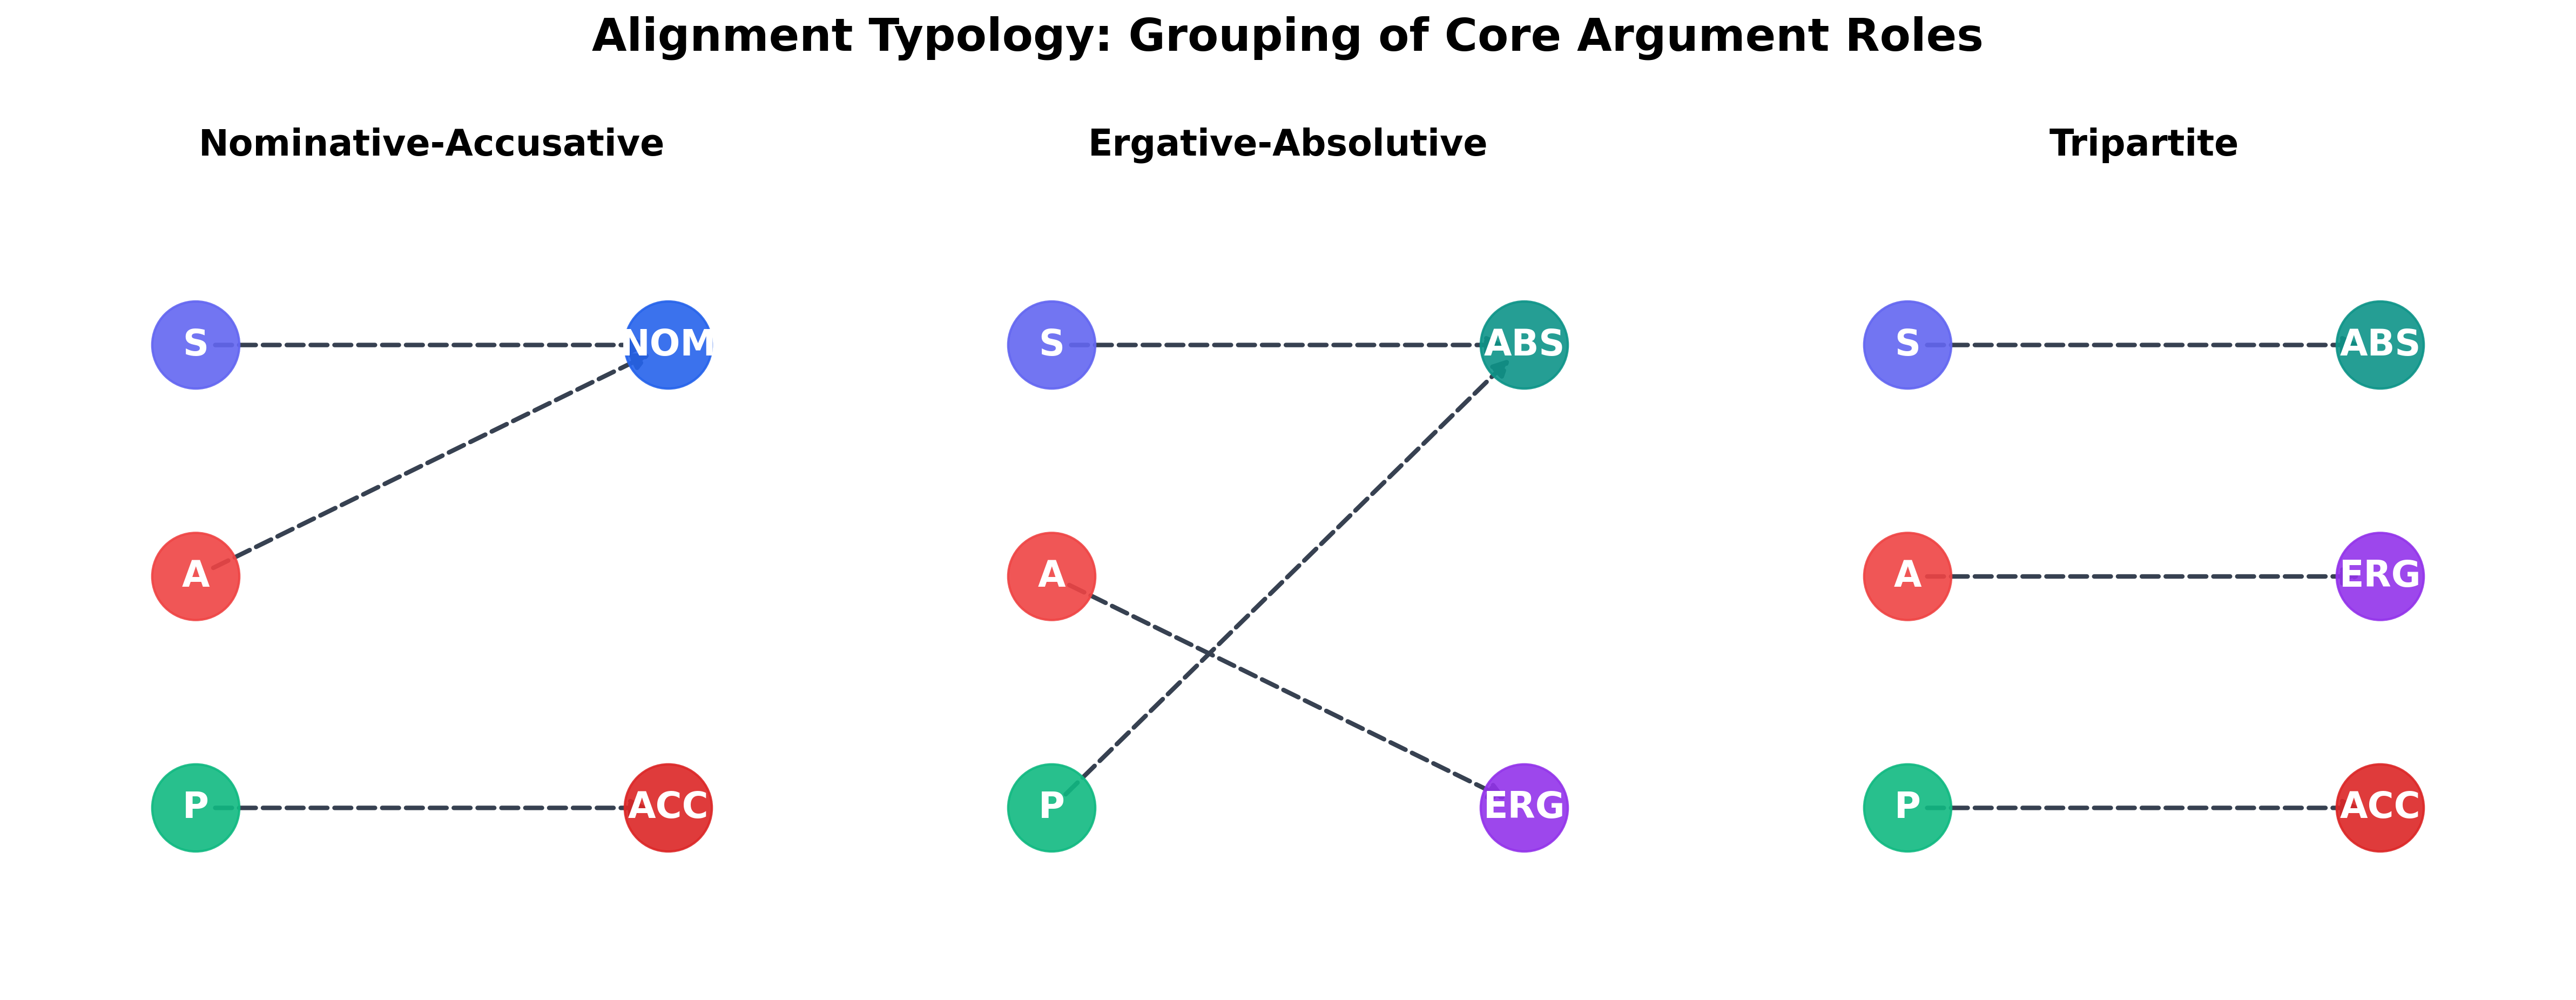
\includegraphics[keepaspectratio,alt={Functor kernels uniquely fingerprint each alignment typology. Three alignment systems realized as functors from \textbackslash mathcal\{U\} = \textbackslash\{S, A, P\textbackslash\}: Nominative--Accusative merges \textbackslash\{S,A\textbackslash\} \textbackslash to \textbackslash text\{NOM\} (kernel \textbackslash\{(S,A)\textbackslash\}, ); Ergative--Absolutive merges \textbackslash\{S,P\textbackslash\} \textbackslash to \textbackslash text\{ABS\} (kernel \textbackslash\{(S,P)\textbackslash\}, ); Tripartite is injective (kernel \textbackslash emptyset). Color-coded nodes reveal neutralization patterns: shared colors indicate functor identification of roles. Generated programmatically from the CaseCategory implementation.}]{../figures/alignment_comparison.png}}
\caption{Functor kernels uniquely fingerprint each alignment typology.
Three alignment systems realized as functors from
\(\mathcal{U} = \{S, A, P\}\): \textbf{Nominative--Accusative} merges
\(\{S,A\} \to \text{NOM}\) (kernel \(\{(S,A)\}\), \autoref{eq:eq-2-3});
\textbf{Ergative--Absolutive} merges \(\{S,P\} \to \text{ABS}\) (kernel
\(\{(S,P)\}\), \autoref{eq:eq-2-4}); \textbf{Tripartite} is injective
(kernel \(\emptyset\)). Color-coded nodes reveal neutralization
patterns: shared colors indicate functor identification of roles.
Generated programmatically from the \protect\texttt{CaseCategory}
implementation.}\label{fig:alignment}
\end{figure}

\begin{figure}
\centering
\pandocbounded{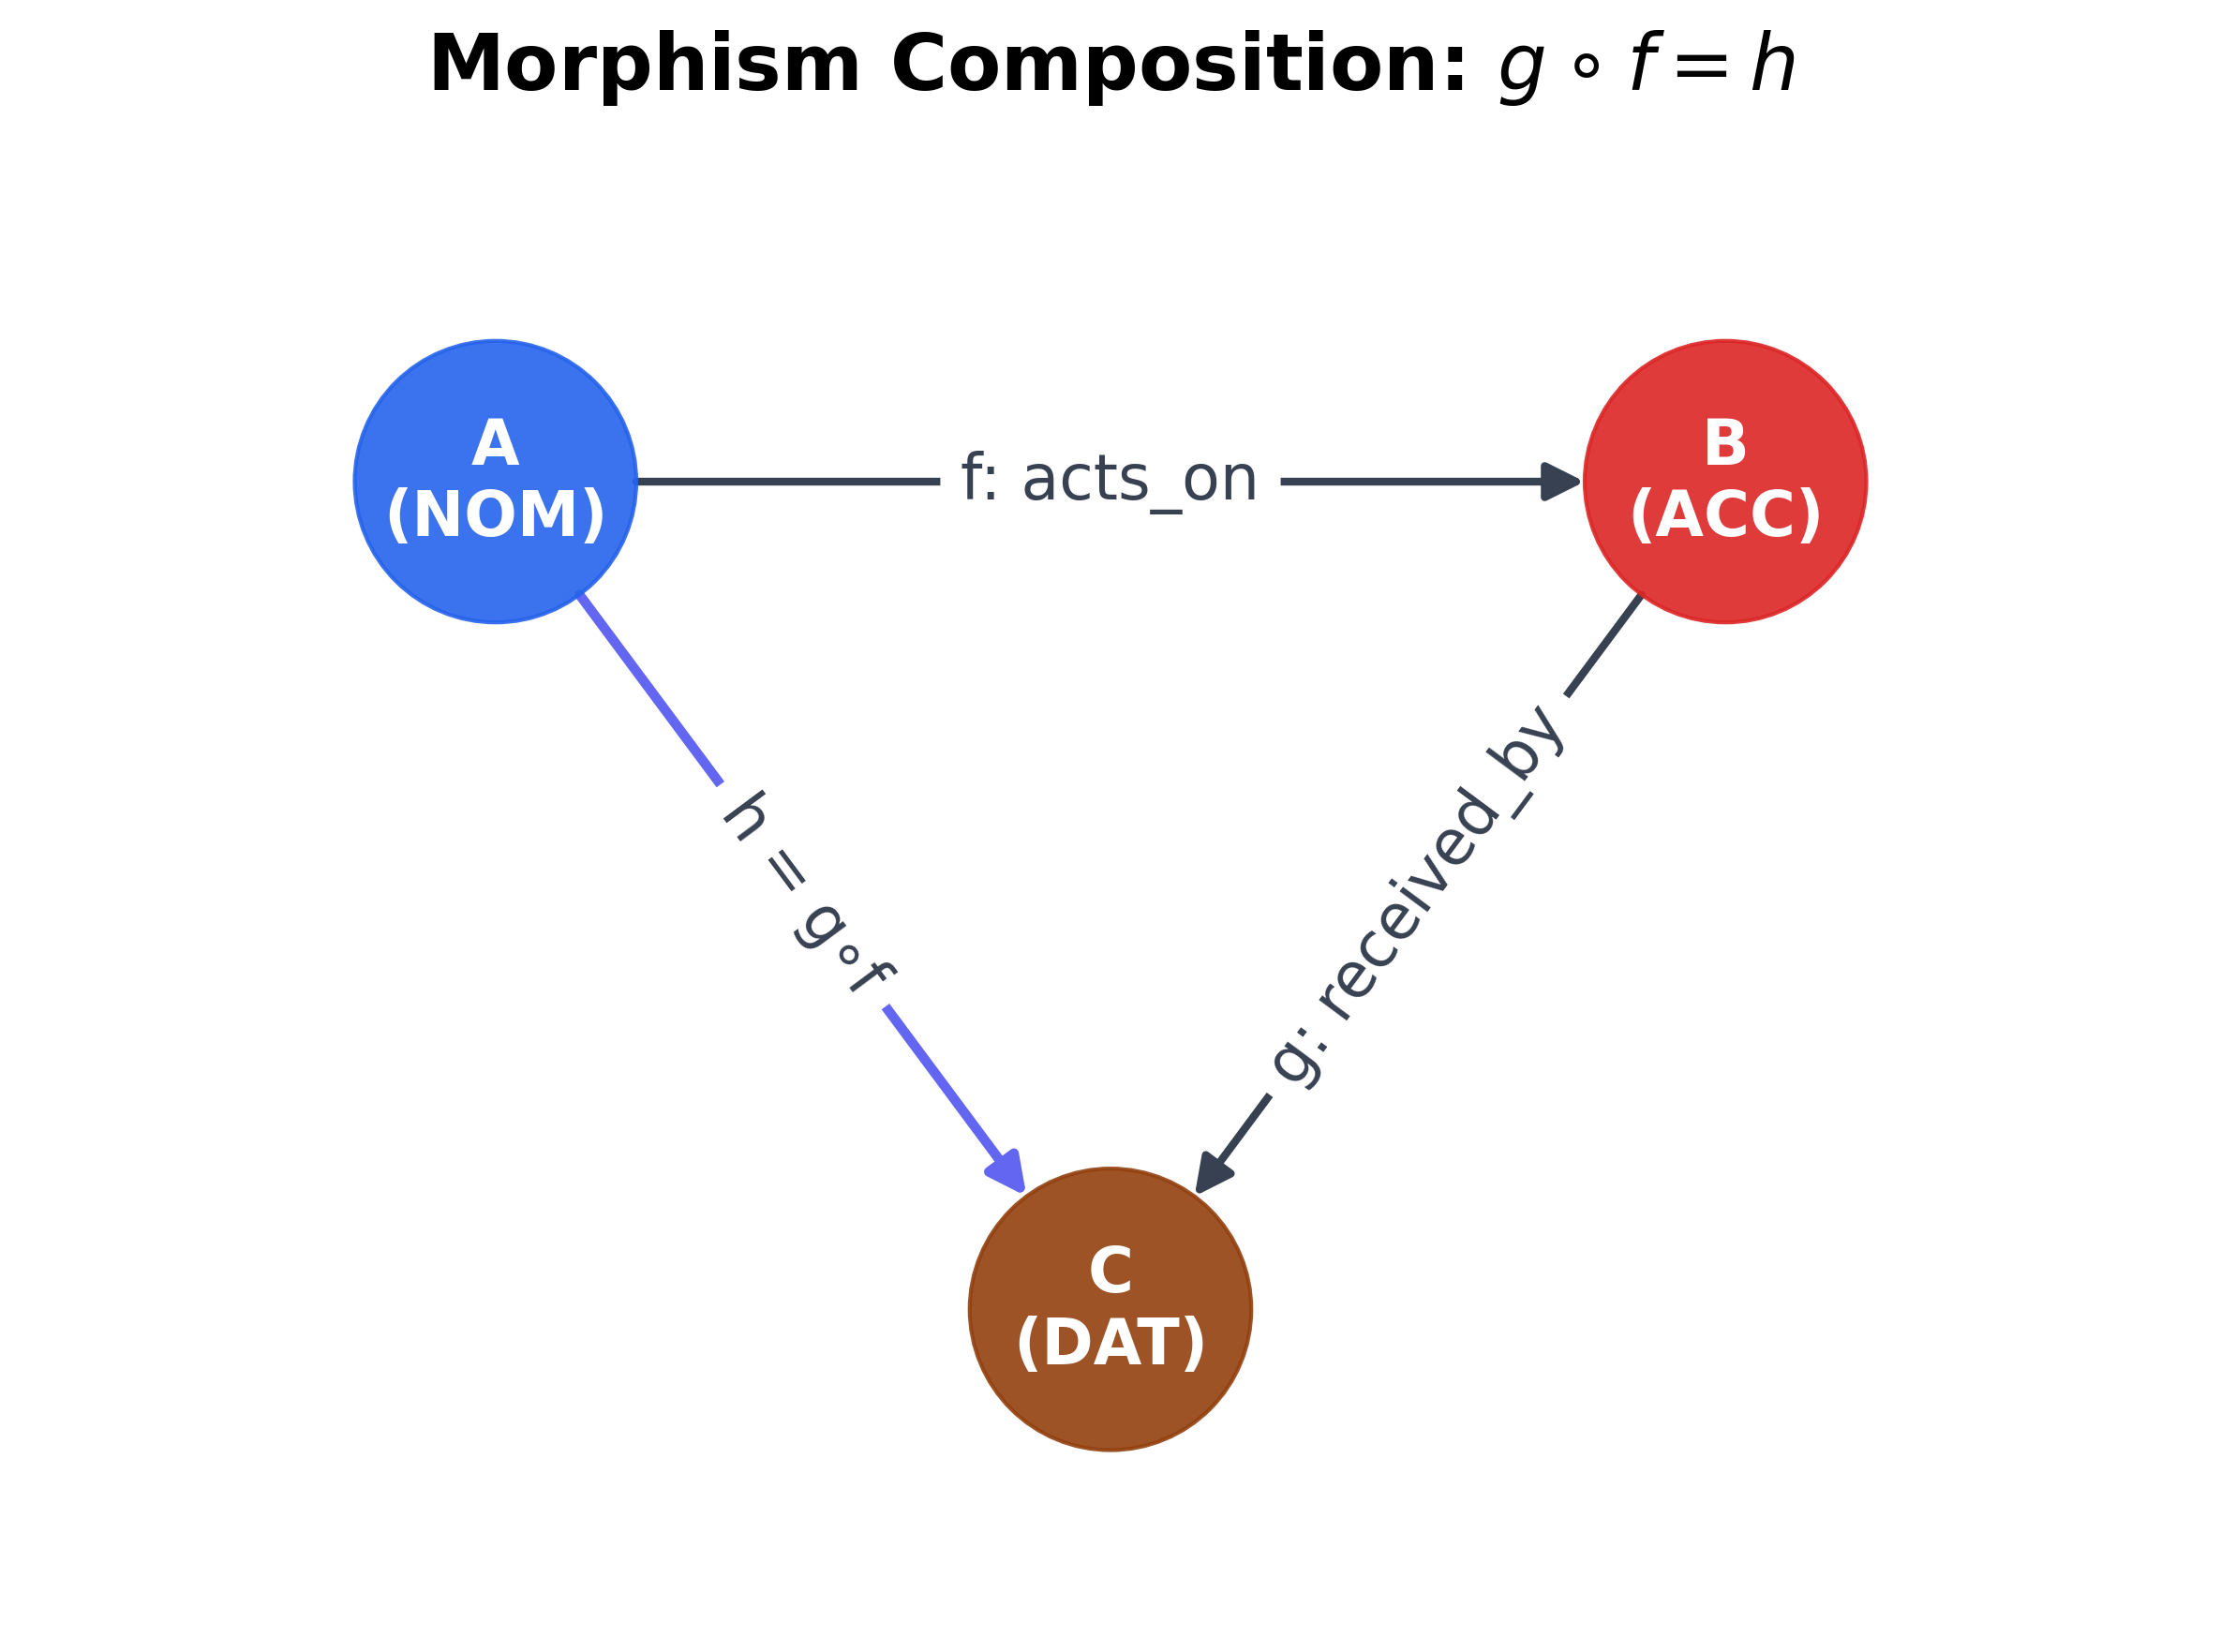
\includegraphics[keepaspectratio,alt={Morphism composition attenuates weights multiplicatively through intermediate case roles. Morphism f\textbackslash colon\textbackslash text\{NOM\}\textbackslash to\textbackslash text\{ACC\} (acts\_on) and g\textbackslash colon\textbackslash text\{ACC\}\textbackslash to\textbackslash text\{DAT\} (received\_by) compose to h = g \textbackslash circ f\textbackslash colon\textbackslash text\{NOM\}\textbackslash to\textbackslash text\{DAT\} per ; in the enriched category weights multiply (e.g., w\_f = 0.9, w\_g = 0.7 \textbackslash Rightarrow w(g \textbackslash circ f) = 0.63). The commutative triangle encodes that DAT assignment factors through ACC---the multiplicative attenuation reflects the typological observation that subject--recipient relations are weaker than the constituent subject--object and object--recipient links. Generated programmatically from the CaseCategory class.}]{../figures/composition_triangle.png}}
\caption{Morphism composition attenuates weights multiplicatively
through intermediate case roles. Morphism
\(f\colon\text{NOM}\to\text{ACC}\) (acts\_on) and
\(g\colon\text{ACC}\to\text{DAT}\) (received\_by) compose to
\(h = g \circ f\colon\text{NOM}\to\text{DAT}\) per \autoref{eq:eq-2-1};
in the enriched category weights multiply (e.g., \(w_f = 0.9\),
\(w_g = 0.7 \Rightarrow w(g \circ f) = 0.63\)). The commutative triangle
encodes that DAT assignment factors through ACC---the multiplicative
attenuation reflects the typological observation that subject--recipient
relations are weaker than the constituent subject--object and
object--recipient links. Generated programmatically from the
\protect\texttt{CaseCategory} class.}\label{fig:composition}
\end{figure}

\subsection{\texorpdfstring{Graded Proto-Roles as \([0,1]\)-Weighted
Morphisms}{Graded Proto-Roles as {[}0,1{]}-Weighted Morphisms}}\label{graded-proto-roles-as-01-weighted-morphisms}

Following Dowty \citeyearpar{dowty1991thematic}, we equip morphisms with
weights in \([0,1]\) that encode the degree of proto-role satisfaction.
A morphism \(f: \text{NOM} \to \text{ACC}\) with weight \(w = 0.9\)
indicates a strong transitive action (clear agent acting on clear
patient), while \(w = 0.4\) might indicate an experiencer construction
(``The child fears the dark'') where the nominative argument only weakly
satisfies Proto-Agent entailments.

\textbf{Slavic quirky case as overt evidence for sub-unit morphism
weights.} Russian and Serbian/BCS supply a sharper,
\emph{morphologically overt} witness for \(w < 1\): a class of verbs
that systematically refuses the canonical NOM \(\to\) ACC arrow and
instead routes its object through GEN, DAT, or INS. In Russian,
\emph{boyat'sja} ``to fear'' governs the genitive (\emph{boyus' sobaki}
``I fear the dog-GEN'', not *\emph{sobaku}-ACC); \emph{pomogat'} ``to
help'' governs the dative (\emph{pomogayu drugu} ``I help the
friend-DAT''); \emph{upravlyat'} ``to manage / steer'' governs the
instrumental (\emph{upravlyaet mašinoj} ``drives the car-INS'').
Serbian/BCS shows the same pattern: \emph{čestitati} ``to congratulate''
assigns DAT (\emph{čestitam prijatelju} ``I congratulate the
friend-DAT''); \emph{bojati se} ``to fear'' assigns GEN (\emph{bojim se
psa} ``I fear the dog-GEN''). Each such verb supplies an enriched
morphism whose target is \emph{not} ACC, equivalently a NOM \(\to\) ACC
arrow whose Dowtian weight has been reduced to near zero --- and the
reduction is visible in the suffix on the noun, not merely hypothesised
from semantics. These quirky-case lexemes are the cleanest empirical
anchor for the graded \([0,1]\)-enrichment we develop in
\autoref{sec:enriched-categories}.

Composition of enriched morphisms multiplies weights: \begin{equation}
w(g \circ f) = w(g) \cdot w(f)
\label{eq:eq-2-1}
\end{equation}

This multiplicative composition reflects the intuition that grammatical
dependencies attenuate as they chain through intermediate roles.
\autoref{fig:composition} illustrates the categorical composition of two
morphisms through an intermediate case role. The resulting structure is
a category enriched over \(([0,1], \cdot, 1)\)---a connection we develop
fully in \autoref{sec:enriched-categories}.

\subsection{Alignment Shifts as Natural Transformations: Functor
Commutativity Encodes Grammar
Agreement}\label{alignment-shifts-as-natural-transformations-functor-commutativity-encodes-grammar-agreement}

Having established that alignment systems are functors
\(F, G: \mathcal{U} \to \mathcal{L}\) from a universal case category to
language-specific categories, a natural question arises: \emph{how do
different alignment systems relate to each other?} The categorical
answer is a \textbf{natural transformation}
\(\alpha: F \Rightarrow G\)---a systematic family of morphisms
\(\alpha_A: F(A) \to G(A)\) for each case role \(A\), satisfying the
\textbf{naturality condition}:

\begin{equation}
G(f) \circ \alpha_A = \alpha_B \circ F(f) \quad \text{for every morphism } f: A \to B
\label{eq:eq-2-2}
\end{equation}

This naturality constraint is the formal expression of \emph{grammatical
coherence}: transforming one alignment into another and then applying a
grammatical relation yields the same result as first applying the
relation and then transforming---ensuring that alignment comparison
respects the relational fabric of the grammar.

\textbf{Worked example.} Consider the accusative functor \(F\) (which
maps S and A to NOM, P to ACC) alongside the tripartite functor \(G\)
(which maps explicitly to S \(\to\) ABS, A \(\to\) ERG, P \(\to\) ACC).
The \textbf{identity natural transformation}
\(\text{id}_F: F \Rightarrow F\) provides components
\({(\text{id}_F)}_A = \text{id}_{F{(A)}}\) over every role \(A\),
trivially satisfying the naturality condition. We construct the
\textbf{vertical composition} \(\beta \circ \alpha{}\) of two natural
transformations \(\alpha: F \Rightarrow G\) and
\(\beta: G \Rightarrow H\) purely componentwise:
\({(\beta \circ \alpha)}_A = \beta_A \circ \alpha_A\).

Our \texttt{NaturalTransformation} class implements these operations,
with \texttt{ComponentMorphism} objects encoding each \(\alpha_A\), and
\texttt{compose\_transformations()} implementing vertical composition.
The \texttt{IdentityNaturalTransformation} constructor automatically
generates identity components for every object in an
\texttt{AlignmentFunctor}'s domain. This machinery provides the formal
infrastructure for comparing alignment types not merely by listing their
neutralization patterns but by characterizing the \emph{structural
mappings} between them---e.g., the natural transformation from
accusative to tripartite alignment is injective (no two roles merge in
the target), while the transformation from tripartite to ergative is
non-injective (S and P merge into ABS).

\newpage

\section{Categorial Grammar: Syntax as Algebraic Composition and
Proof}\label{sec:categorial-grammar}

\textbf{Where we are in the argument.} \autoref{sec:case-categories}
built the case category --- a static snapshot of licensed role-to-role
morphisms. This chapter equips the framework with a \emph{compositional
syntax} on top of that static layer: Lambek pregroup types let each word
carry its own combinatory potential, and cup/cap contractions reduce a
parallel tensor of word-boxes to the single sentence type \(s\), so a
sentence becomes a proof of well-typedness rendered graphically as a
string diagram.

\subsection{Each Word Is Its Own Grammar
Rule}\label{each-word-is-its-own-grammar-rule}

Traditional generative grammar computes sentence structure using
top-down phrase-structure rules that recursively combine constituents.
Categorial grammar inverts this perspective: rather than specifying
abstract construction rules, it assigns each lexical item a dedicated
\emph{type} that encodes its combinatory potential. For example, a
transitive verb like ``chases'' is not loosely defined as ``a word
requiring a subject and object,'' but specifically assigned the
algebraic type \((n \backslash s) / n\)---an active function that
categorically demands a noun to its right (the object) and a noun to its
left (the subject) to yield a complete sentence.

\subsection{Lambek's Residuation Law: Consuming and Producing Types in
Linear
Order}\label{lambeks-residuation-law-consuming-and-producing-types-in-linear-order}

Lambek \citeyearpar{lambek1958mathematics} laid the algebraic
foundations by introducing a \emph{residuated} structure on syntactic
types. He defined two binary operations---the left residual
\(\backslash\) and the right residual \(/\)---derived from the
multiplicative connective \(\otimes\) (concatenation). The fundamental
axiom governing this system is the residuation law:

\begin{equation}
A \otimes B \leq C \quad \iff \quad A \leq C / B \quad \iff \quad B \leq A \backslash C
\label{eq:eq-3-1}
\end{equation}

This law brilliantly captures the fundamental duality of syntax: a verb
of type \((n \backslash s) / n\) actively \emph{consumes} available noun
arguments to \emph{produce} a well-formed sentence. The resulting
\textbf{Lambek calculus} operates as a non-commutative intuitionistic
linear logic---non-commutative because strict word order dictates
meaning, and linear because the derivation logically consumes each
lexical resource exactly once.

\subsubsection{Pregroups Unlock Compact Closure: The Bridge to DisCoCat
String
Diagrams}\label{pregroups-unlock-compact-closure-the-bridge-to-discocat-string-diagrams}

Lambek \citeyearpar{lambek2004fine} later simplified the framework to
\textbf{pregroup grammars}, where each type \(a\) has a left adjoint
\(a^l\) and a right adjoint \(a^r\) satisfying:

\begin{equation}
a^l \cdot a \leq 1 \leq a \cdot a^l \qquad a \cdot a^r \leq 1 \leq a^r \cdot a
\label{eq:eq-3-2}
\end{equation}

Coecke, Sadrzadeh, and Clark revolutionized this formal structuralism in
2010 with the \textbf{DisCoCat} (Distributional Compositional
Categorical) model \citeyearpar{coecke2010mathematical}. DisCoCat
mathematically unifies categorial grammar with distributional semantics
by defining strong monoidal functors mapping pregroup grammars directly
into vector spaces. As Duneau emphasizes, this approach ``allows the
meaning of a sentence to be computed as a function of both the
distributional meaning of the words involved, as well as its grammatical
form'' \citeyearpar{duneau2021parsing}. By proving that pregroups and
finite-dimensional vector spaces both behave as rigid monoidal
categories, DisCoCat allows us to compute whole-sentence vector meanings
linearly from constituent word vectors.

In this system, grammaticality reduces to algebraic verification:
checking whether a sequence of types maps to the sentence type \(s\) via
\emph{contraction} (\(a^l \cdot a \to 1\)) and \emph{expansion}
(\(1 \to a \cdot a^l\)) operations. This reformulation unlocks the
DisCoCat framework (\autoref{sec:categorical-semantics}) because
pregroups function as \textbf{compact closed categories}, natively
supporting a computationally sound diagrammatic calculus. When a
derivation is ill-typed, contractions fail to close: there is no valid
reduction to \(s\). \autoref{sec:cognitive-security} develops the
security reading of that failure mode---typed interaction boundaries and
prompt injection as illicit role reassignment.

\subsection{Cups, Caps, and Joyal--Street: How Wires Prove
Grammaticality}\label{cups-caps-and-joyalstreet-how-wires-prove-grammaticality}

The pivotal connection between categorial grammar and visualization
comes from Joyal and Street \citeyearpar{joyalstreet1991geometry}, who
proved that morphisms in monoidal categories can be faithfully
represented as \emph{string diagrams}---planar graphs where:

\begin{itemize}
\tightlist
\item
  \textbf{Wires} represent types (objects of the category)
\item
  \textbf{Boxes} represent words or operations (morphisms)
\item
  \textbf{Vertical composition} represents sequential application
\item
  \textbf{Horizontal juxtaposition} represents the tensor product
  (concatenation)
\item
  \textbf{Cups and caps} represent the contraction/expansion of a
  pregroup
\end{itemize}

\autoref{fig:string-diagram} surveys three syntactic structures side by
side (progression from intransitive to passive);
\autoref{fig:native-discocat} shows the same transitive sentence
rendered by our native matplotlib pipeline---a direct computational
output confirming word-box layout, wire routing, and cup-contraction
geometry independently of DisCoPy; and
\autoref{fig:multilingual-isomorphism} demonstrates that type-logical
structure remains invariant across diverse surface word orders (SVO,
free, SOV).

\begin{figure}
\centering
\pandocbounded{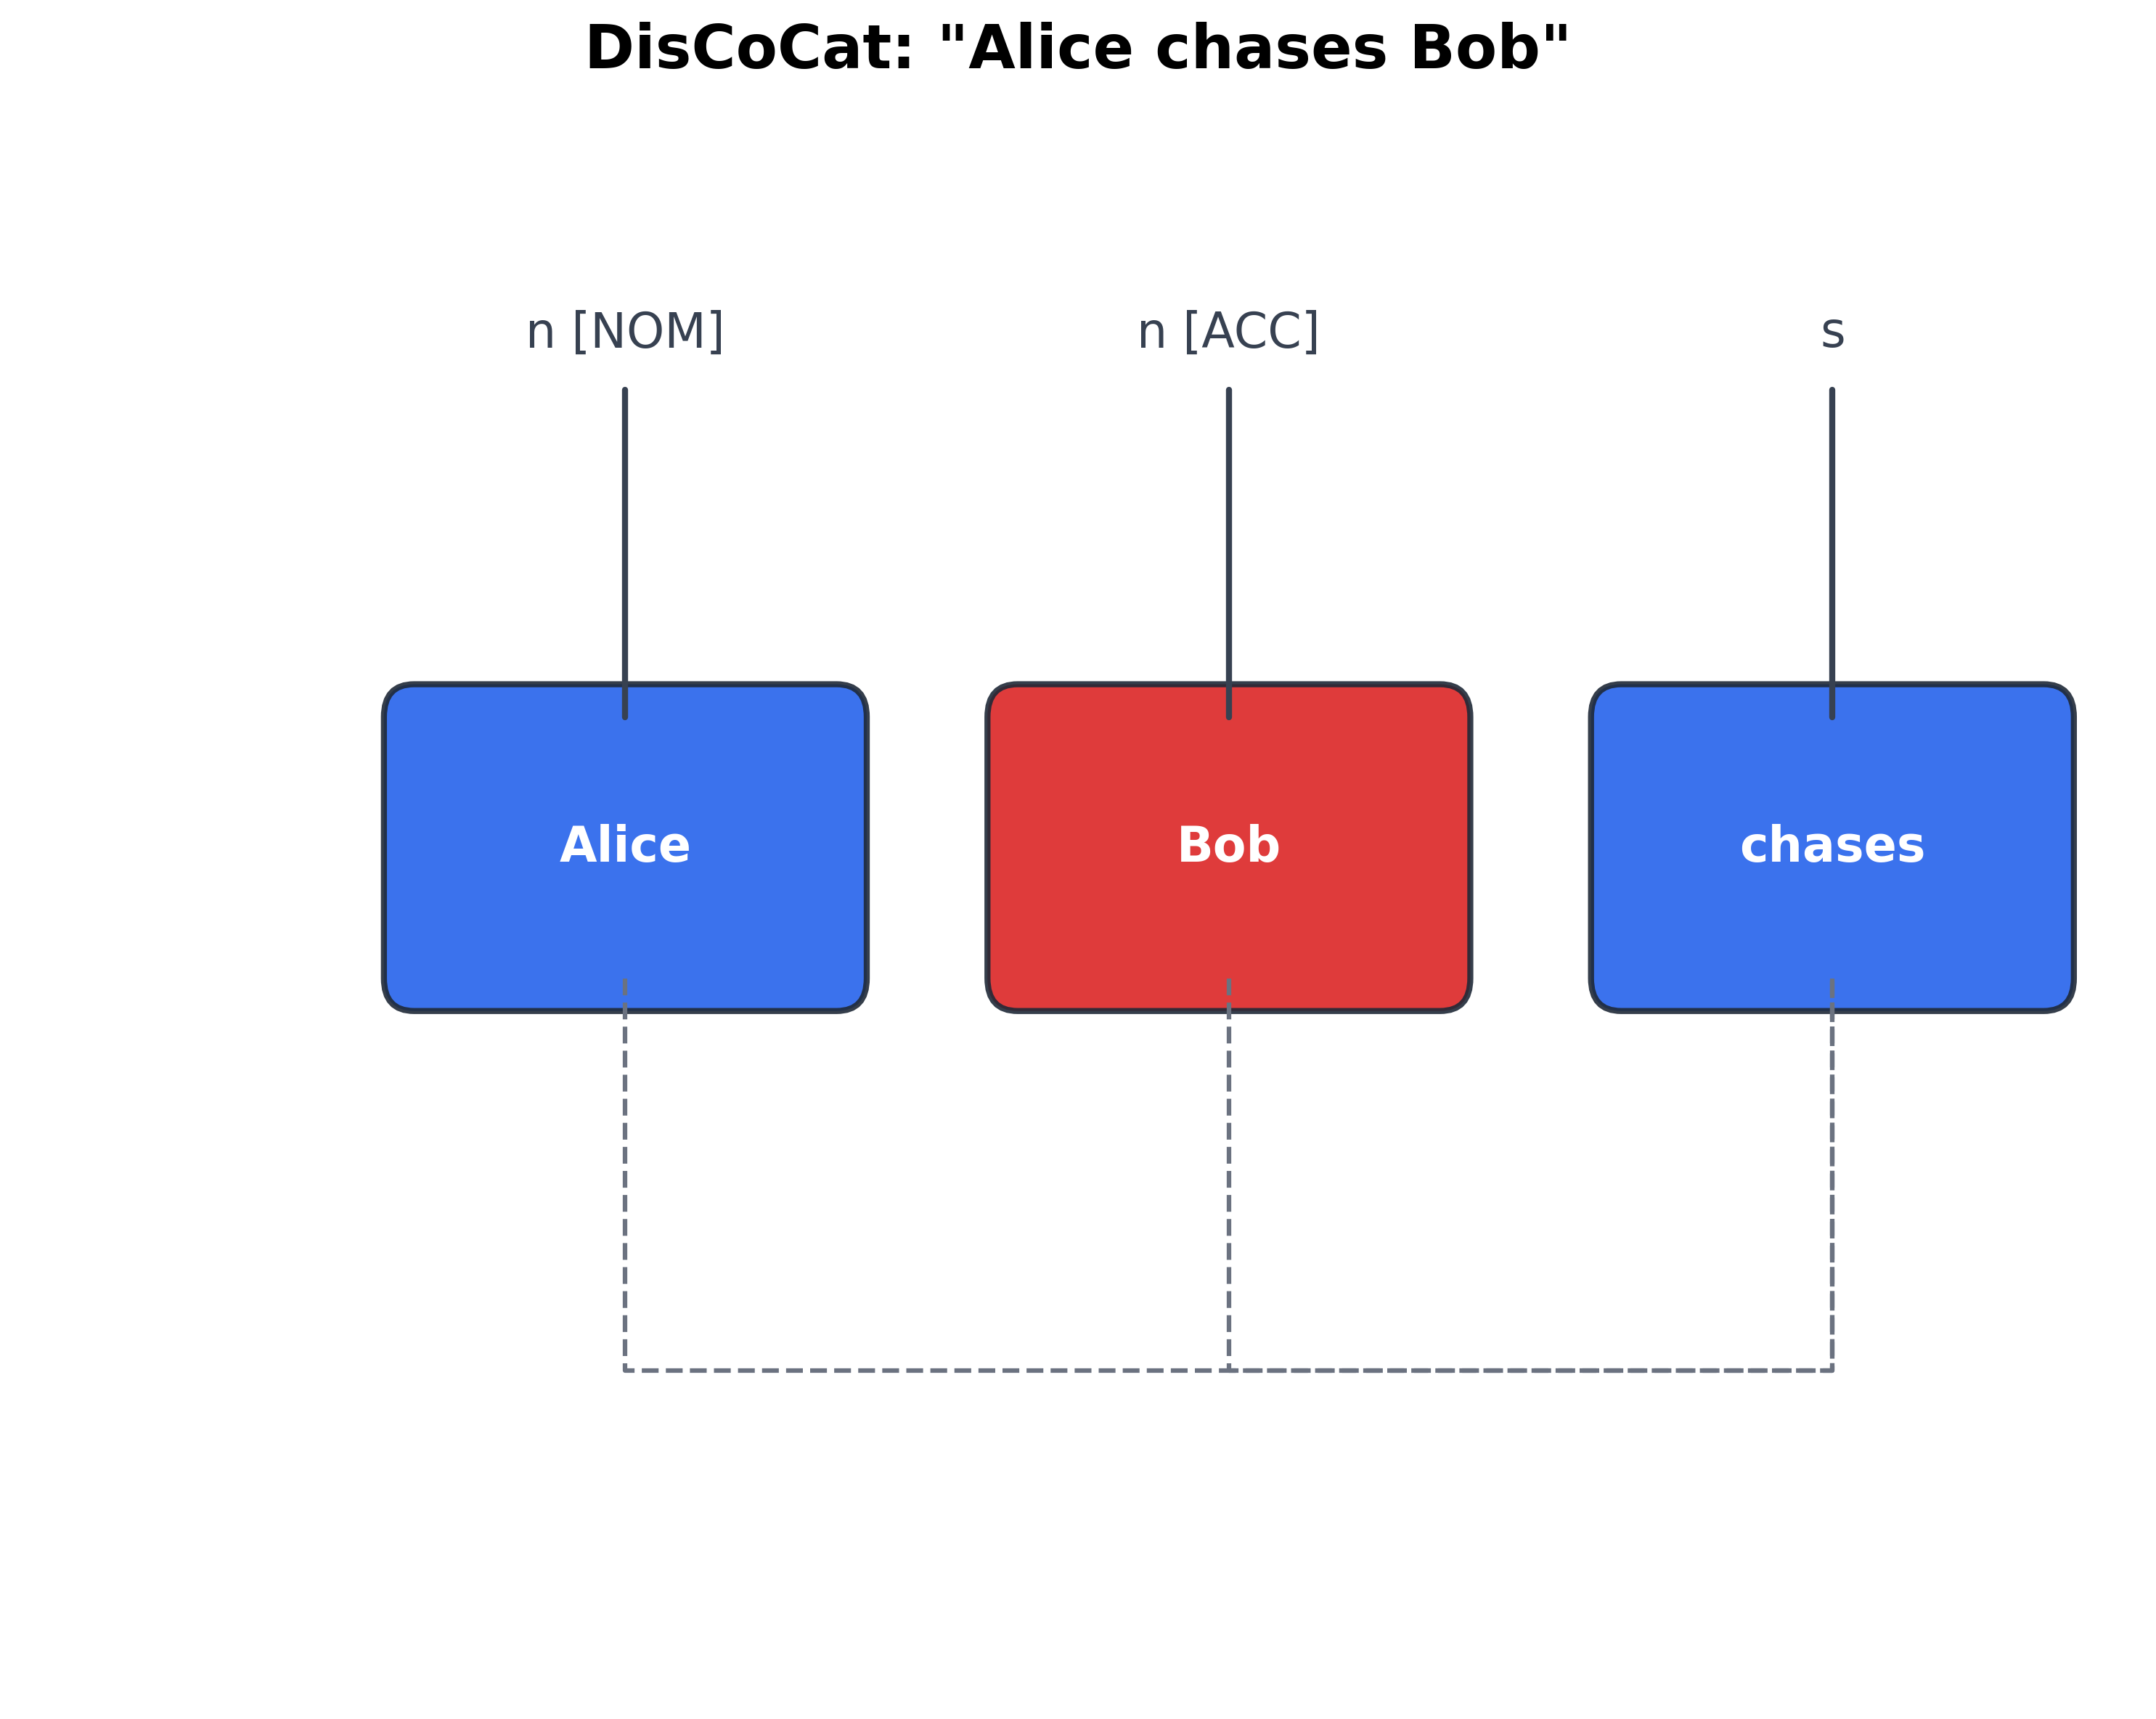
\includegraphics[keepaspectratio,alt={Native matplotlib rendering cross-validates DisCoPy pregroup geometry. String diagram for ``Alice chases Bob'' generated via src.visualization.string\_diagrams.render\_discocat\_sentence() without the DisCoPy library. Three Word boxes carry pregroup types: n (Alice, blue = NOM), n\^{}r \textbackslash otimes s \textbackslash otimes n\^{}l (chases, neutral), and n (Bob, red = ACC). Dashed arcs trace cup connections from noun wires to the verb's adjoint slots, rendering \textbackslash varepsilon: n\^{}r \textbackslash otimes n \textbackslash to 1 and \textbackslash varepsilon: n\^{}l \textbackslash otimes n \textbackslash to 1 as paired ligatures. This confirms that our visualization pipeline correctly reconstructs pregroup string-diagram geometry using only case-role metadata from src.case\_systems.case\_category, cross-validating the DisCoPy canonical output in .}]{../figures/string_diagram_discocat.png}}
\caption{Native matplotlib rendering cross-validates DisCoPy pregroup
geometry. String diagram for ``Alice chases Bob'' generated via
\protect\texttt{src.visualization.string\_diagrams.render\_discocat\_sentence()}
without the DisCoPy library. Three Word boxes carry pregroup types:
\(n\) (Alice, \textbf{blue} = NOM), \(n^r \otimes s \otimes n^l\)
(chases, \textbf{neutral}), and \(n\) (Bob, \textbf{red} = ACC). Dashed
arcs trace cup connections from noun wires to the verb's adjoint slots,
rendering \(\varepsilon: n^r \otimes n \to 1\) and
\(\varepsilon: n^l \otimes n \to 1\) as paired ligatures. This confirms
that our visualization pipeline correctly reconstructs pregroup
string-diagram geometry using only case-role metadata from
\protect\texttt{src.case\_systems.case\_category}, cross-validating the
DisCoPy canonical output in
\autoref{fig:discopy-transitive}.}\label{fig:native-discocat}
\end{figure}

\begin{figure}
\centering
\pandocbounded{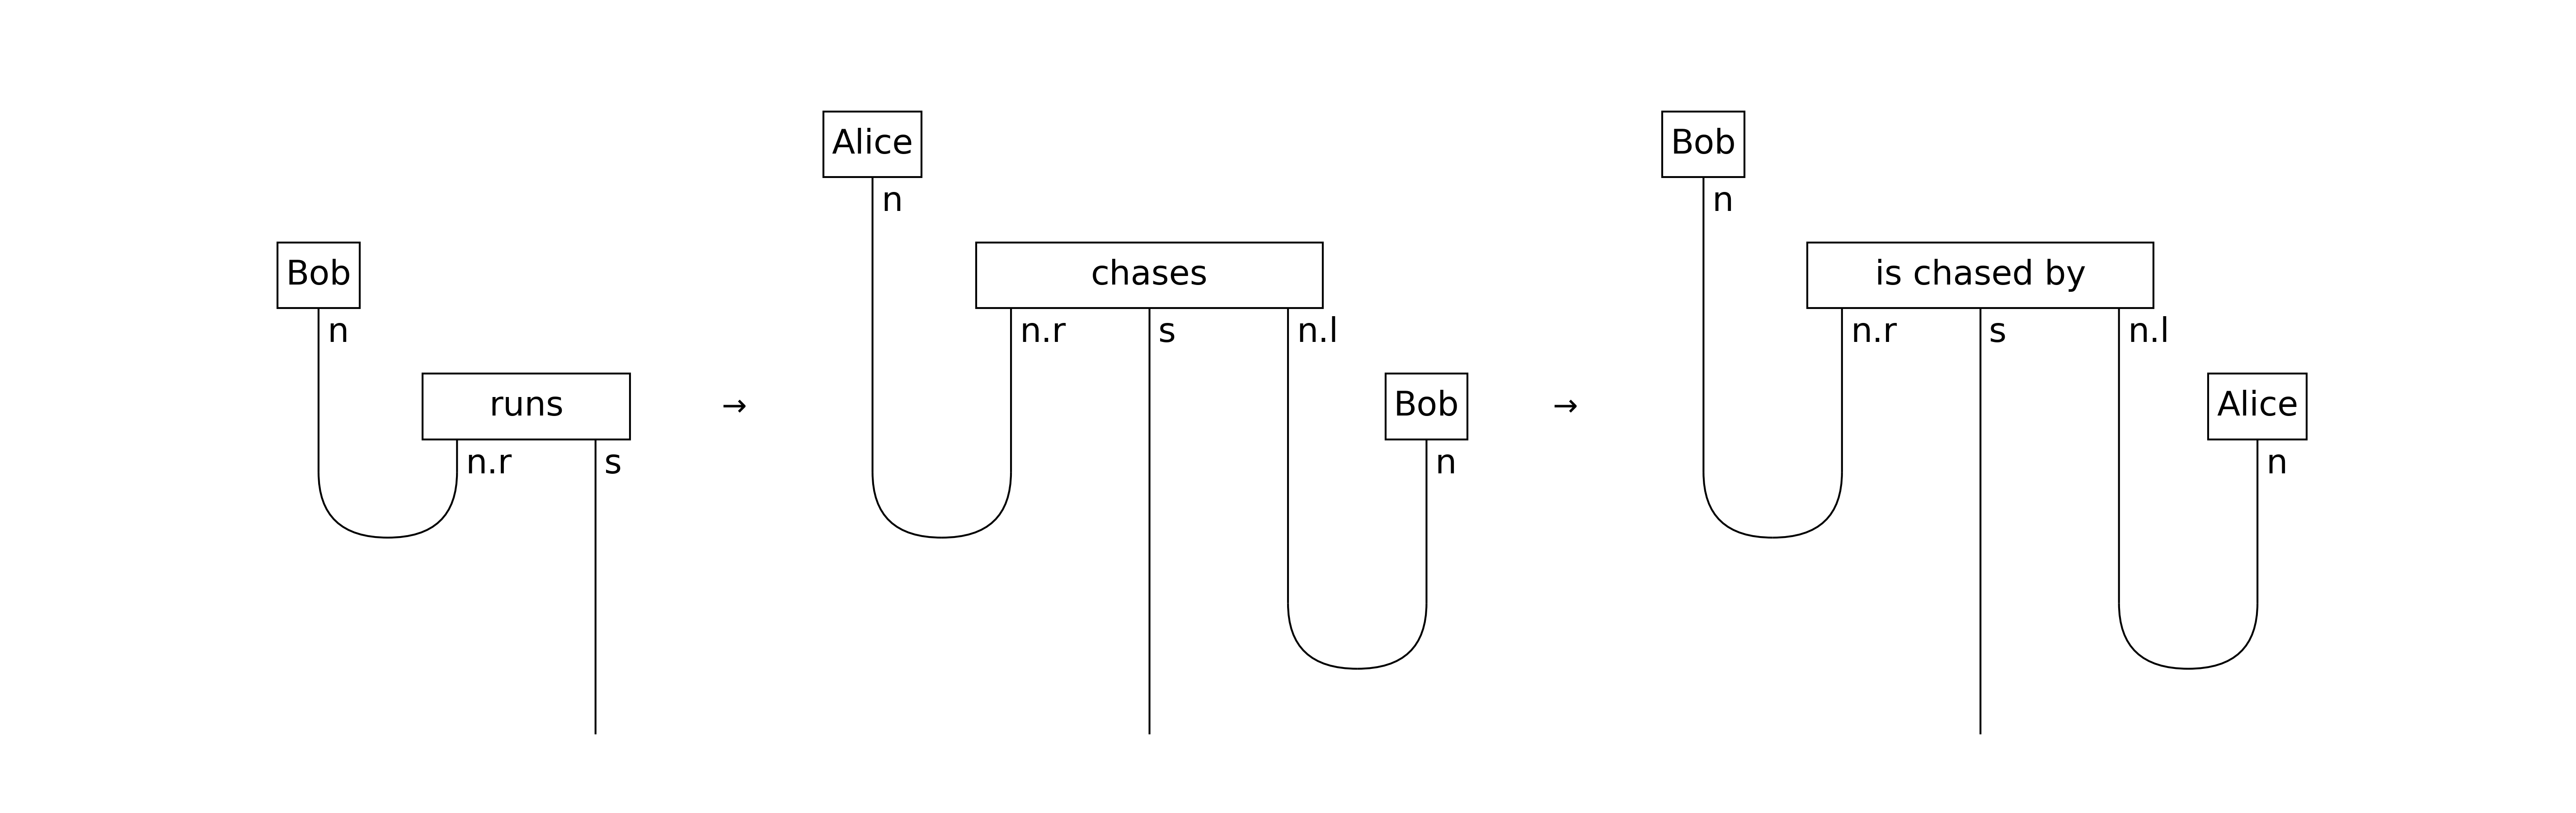
\includegraphics[keepaspectratio,alt={Valency determines diagram topology: Cup count tracks verb argument structure. A 1\texorpdfstring{\ensuremath{\times}}{x}3 DisCoPy pregroup grammar visualization of increasing argument complexity. Panel (a) intransitive ``Bob runs'' (NOM subject, 1 Cup contraction, type n \textbackslash otimes (n\^{}r \textbackslash otimes s) \textbackslash to s); Panel (b) transitive ``Alice chases Bob'' (NOM + ACC, 2 Cup contractions, type n \textbackslash otimes (n\^{}r \textbackslash otimes s \textbackslash otimes n\^{}l) \textbackslash otimes n \textbackslash to s); Panel (c) passive ``Bob is chased by Alice'' (patient promoted to NOM, former agent demoted to an oblique by-phrase; full transitive-shape verb type n\^{}r \textbackslash otimes s \textbackslash otimes n\^{}l with 2 Cup contractions --- which noun enters each cup is reversed relative to panel (b)). The role reassignment is visible as a topological swap of which noun lands in the left (subject) cup and which in the right (oblique) cup; cup count itself encodes argument-slot count, not syntactic prominence. Complexity metric \textbackslash kappa(D) per .}]{../figures/discopy_sentence_progression.png}}
\caption{Valency determines diagram topology: Cup count tracks verb
argument structure. A 1\texorpdfstring{\ensuremath{\times}}{x}3 DisCoPy pregroup grammar visualization of
increasing argument complexity. \textbf{Panel (a)} intransitive ``Bob
runs'' (NOM subject, 1 Cup contraction, type
\(n \otimes (n^r \otimes s) \to s\)); \textbf{Panel (b)} transitive
``Alice chases Bob'' (NOM + ACC, 2 Cup contractions, type
\(n \otimes (n^r \otimes s \otimes n^l) \otimes n \to s\));
\textbf{Panel (c)} passive ``Bob is chased by Alice'' (patient promoted
to NOM, former agent demoted to an oblique \emph{by}-phrase; full
transitive-shape verb type \(n^r \otimes s \otimes n^l\) with 2 Cup
contractions --- \emph{which} noun enters each cup is reversed relative
to panel (b)). The role reassignment is visible as a topological swap of
which noun lands in the left (subject) cup and which in the right
(oblique) cup; cup count itself encodes argument-slot count, not
syntactic prominence. Complexity metric \(\kappa(D)\) per
\autoref{eq:eq-4-4}.}\label{fig:string-diagram}
\end{figure}

\begin{figure}
\centering
\pandocbounded{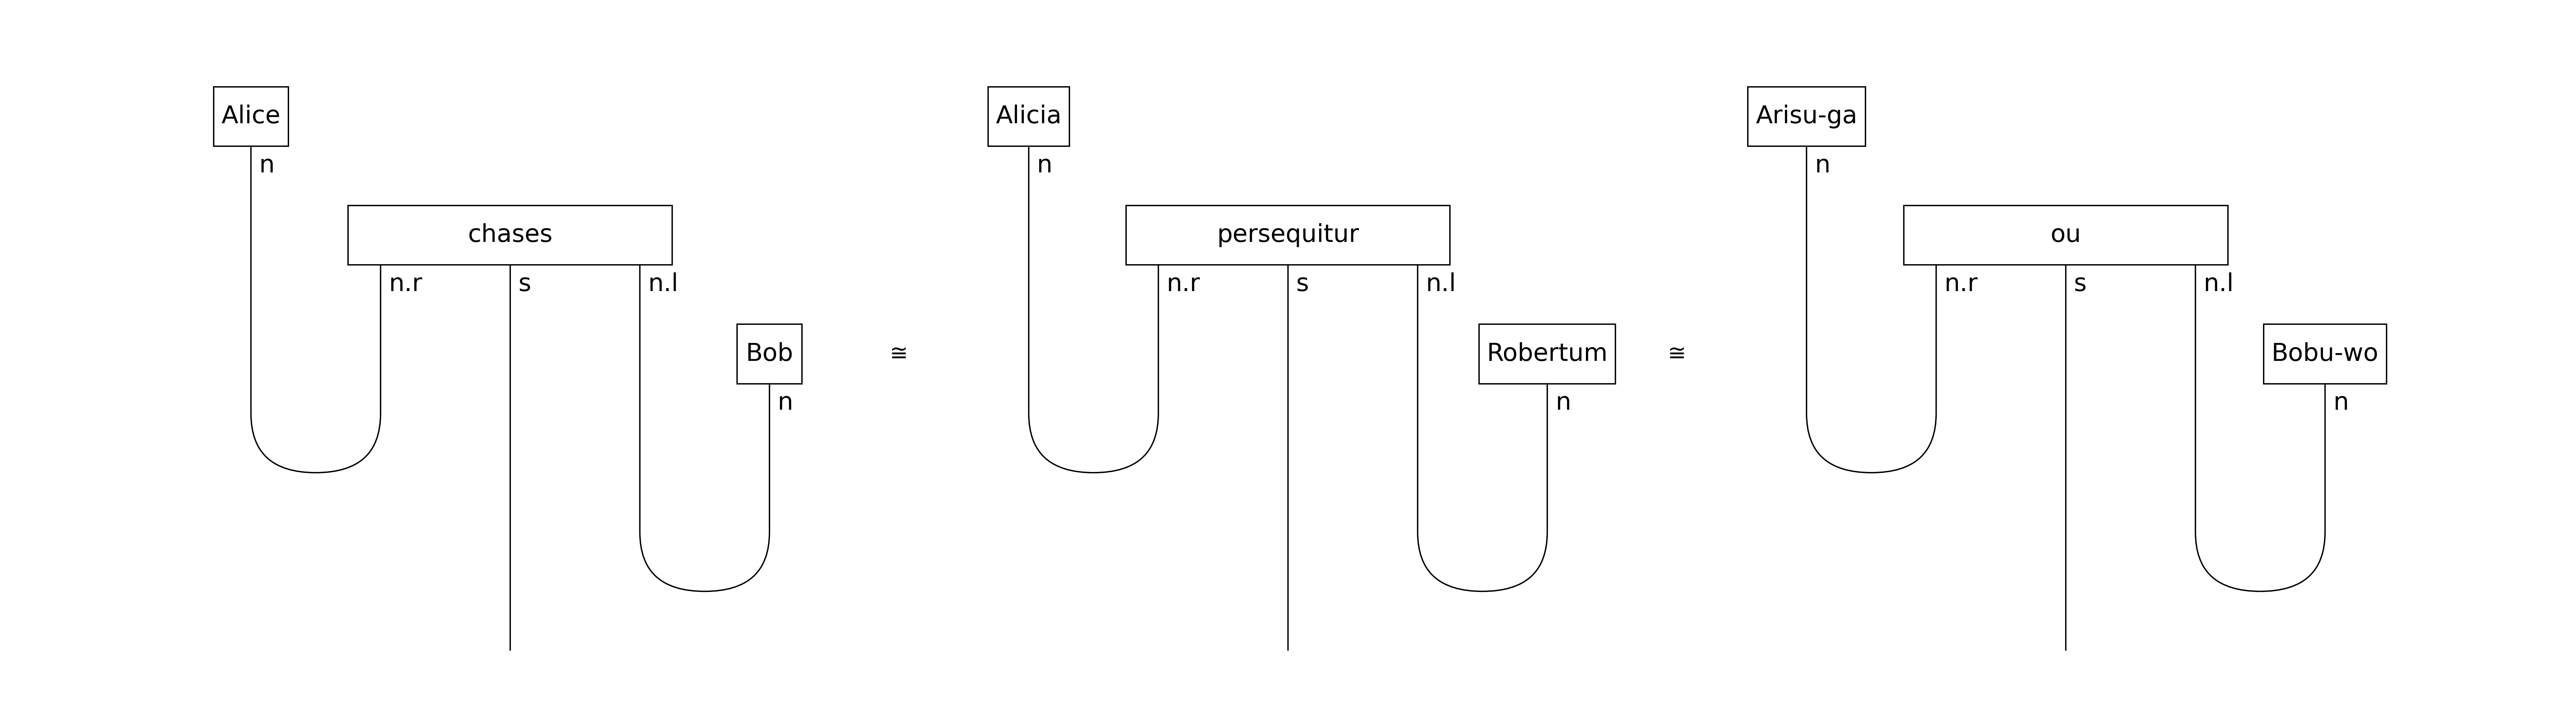
\includegraphics[keepaspectratio,alt={Type-logical structure is invariant under surface word-order permutation. Pregroup derivations for ``SUBJ chases OBJ'' across three typologically diverse languages: English (SVO), Latin (inflected, free order), and Japanese (agglutinative, SOV). Each renders an identical type reduction n \textbackslash otimes (n\^{}r \textbackslash otimes s \textbackslash otimes n\^{}l) \textbackslash otimes n \textbackslash to s, confirming the central claim of categorial grammar: syntactic universals reside in the type algebra, not in linear word order.}]{../figures/discopy_multilingual.png}}
\caption{Type-logical structure is invariant under surface word-order
permutation. Pregroup derivations for ``SUBJ chases OBJ'' across three
typologically diverse languages: English (SVO), Latin (inflected, free
order), and Japanese (agglutinative, SOV). Each renders an identical
type reduction
\(n \otimes (n^r \otimes s \otimes n^l) \otimes n \to s\), confirming
the central claim of categorial grammar: syntactic universals reside in
the type algebra, not in linear word
order.}\label{fig:multilingual-isomorphism}
\end{figure}

The Latin point in \autoref{fig:multilingual-isomorphism} generalises
directly to highly inflected modern Slavic. Russian \emph{Sobaka kusaet
čeloveka} ``the dog bites the man'' and its scrambled counterpart
\emph{Čeloveka kusaet sobaka} differ in linear order but share the
reduction
\(n_{\text{NOM}} \otimes (n^r \otimes s \otimes n^l) \otimes n_{\text{ACC}} \to s\),
with the case suffixes (-a NOM.SG.F vs -a ACC.SG.M.ANIM after stem
hardening) supplying the role information that English encodes
positionally. Serbian/BCS exhibits the same robustness: \emph{Pas ujeda
čoveka} / \emph{Čoveka ujeda pas} / \emph{Pas čoveka ujeda} (and three
further permutations) all type-check to \(s\) because the morphological
case marking on the noun wires uniquely identifies which is NOM and
which is ACC. In Slavic languages the type calculus is therefore not
just \emph{consistent} with the surface order --- the surface order is,
to a first approximation, \emph{immaterial}, with case morphology
carrying the entire wiring diagram explicitly.

This result---the soundness and completeness of string-diagrammatic
reasoning---formally guarantees that any topological conclusion drawn
visually from the diagram is algebraically valid: the diagram is not a
heuristic but a rigorous proof instrument.

This profound visual transparency instantiates exactly the ``free ride''
phenomenon identified by Shimojima \citeyearpar{shimojima1996reasoning}:
a single diagram simultaneously exposes the syntactic derivation, the
deep argument structure, and the compositional flow of semantic
meaning---entirely eliminating the need for sequential, explicit
inference steps.

\textbf{Concrete derivation in DisCoPy.} The type reduction for ``Alice
chases Bob'' is computationally verified using the DisCoPy library's
\texttt{discopy.rigid} module:

\begin{Shaded}
\begin{Highlighting}[]
\ImportTok{from}\NormalTok{ discopy.rigid }\ImportTok{import}\NormalTok{ Ty, Box, Cup, Id}
\NormalTok{n, s }\OperatorTok{=}\NormalTok{ Ty(}\StringTok{\textquotesingle{}n\textquotesingle{}}\NormalTok{), Ty(}\StringTok{\textquotesingle{}s\textquotesingle{}}\NormalTok{)}
\NormalTok{alice }\OperatorTok{=}\NormalTok{ Box(}\StringTok{\textquotesingle{}Alice\textquotesingle{}}\NormalTok{, Ty(), n)}
\NormalTok{chases }\OperatorTok{=}\NormalTok{ Box(}\StringTok{\textquotesingle{}chases\textquotesingle{}}\NormalTok{, Ty(), n.r }\OperatorTok{@}\NormalTok{ s }\OperatorTok{@}\NormalTok{ n.l)}
\NormalTok{bob  }\OperatorTok{=}\NormalTok{ Box(}\StringTok{\textquotesingle{}Bob\textquotesingle{}}\NormalTok{,  Ty(), n)}
\NormalTok{words }\OperatorTok{=}\NormalTok{ alice }\OperatorTok{@}\NormalTok{ chases }\OperatorTok{@}\NormalTok{ bob          }\CommentTok{\# n ⊗ (n.r ⊗ s ⊗ n.l) ⊗ n}
\NormalTok{cups  }\OperatorTok{=}\NormalTok{ Cup(n, n.r) }\OperatorTok{@}\NormalTok{ Id(s) }\OperatorTok{@}\NormalTok{ Cup(n.l, n)}
\NormalTok{diagram }\OperatorTok{=}\NormalTok{ words }\OperatorTok{\textgreater{}\textgreater{}}\NormalTok{ cups               }\CommentTok{\# reduces to s}
\ControlFlowTok{assert}\NormalTok{ diagram.cod }\OperatorTok{==}\NormalTok{ s               }\CommentTok{\# type{-}checks: sentence type}
\end{Highlighting}
\end{Shaded}

The two \texttt{Cup} operations successfully contract \(n\) with \(n^r\)
(resolving the subject--verb link) and \(n^l\) with \(n\) (resolving the
verb--object link). This topological reduction collapses the five-wire
tensor product into a single, valid sentence wire \(s\). Consequently,
the assertion \texttt{diagram.cod\ ==\ s} constitutes a direct,
machine-processable proof of grammaticality.

\textbf{From pregroup types to graded types.} The standard pregroup
derivation produces a rigid, binary grammaticality judgment: the final
codomain of the fully contracted tensor product either matches the
sentence type \(s\) (grammatical) or fails (ill-formed). However, we can
\emph{grade} this binary verdict by replacing the underlying Boolean
algebra \(\{0,1\}\) with the continuous unit interval \([0,1]\). This
substitution yields a graded type theory where type judgments carry
continuous confidence weights rather than truth values. Asudeh and
Giorgolo \citeyearpar{asudeh2020graded} developed this approach using a
monadic semantics that wraps base types inside a computational effect
tracking epistemic uncertainty---an idea whose categorical content is
precisely a change of enrichment base.

Mapped into our framework, this operation corresponds to the
\([0,1]\)-enrichment detailed in \autoref{sec:enriched-categories}: the
enriched scalar weight on any morphism \(f: A \to B\) quantifies the
confidence that the categorical case assignment \(A \to B\) remains
well-typed. From there, categorical magnitude aggregates these sparse,
local confidence scores into a global complexity measure evaluating the
entire syntactic derivation. The progression from rigid pregroup
strings, through graded types, into fully enriched case categories
operates mathematically as a cascade of base-change functors
(\(\mathbf{Bool} \hookrightarrow [0,1] \hookrightarrow \mathbf{R}_{\geq 0}\))---where
each successive level grants greater representational nuance while
demanding higher computational complexity.

\begin{figure}
\centering
\pandocbounded{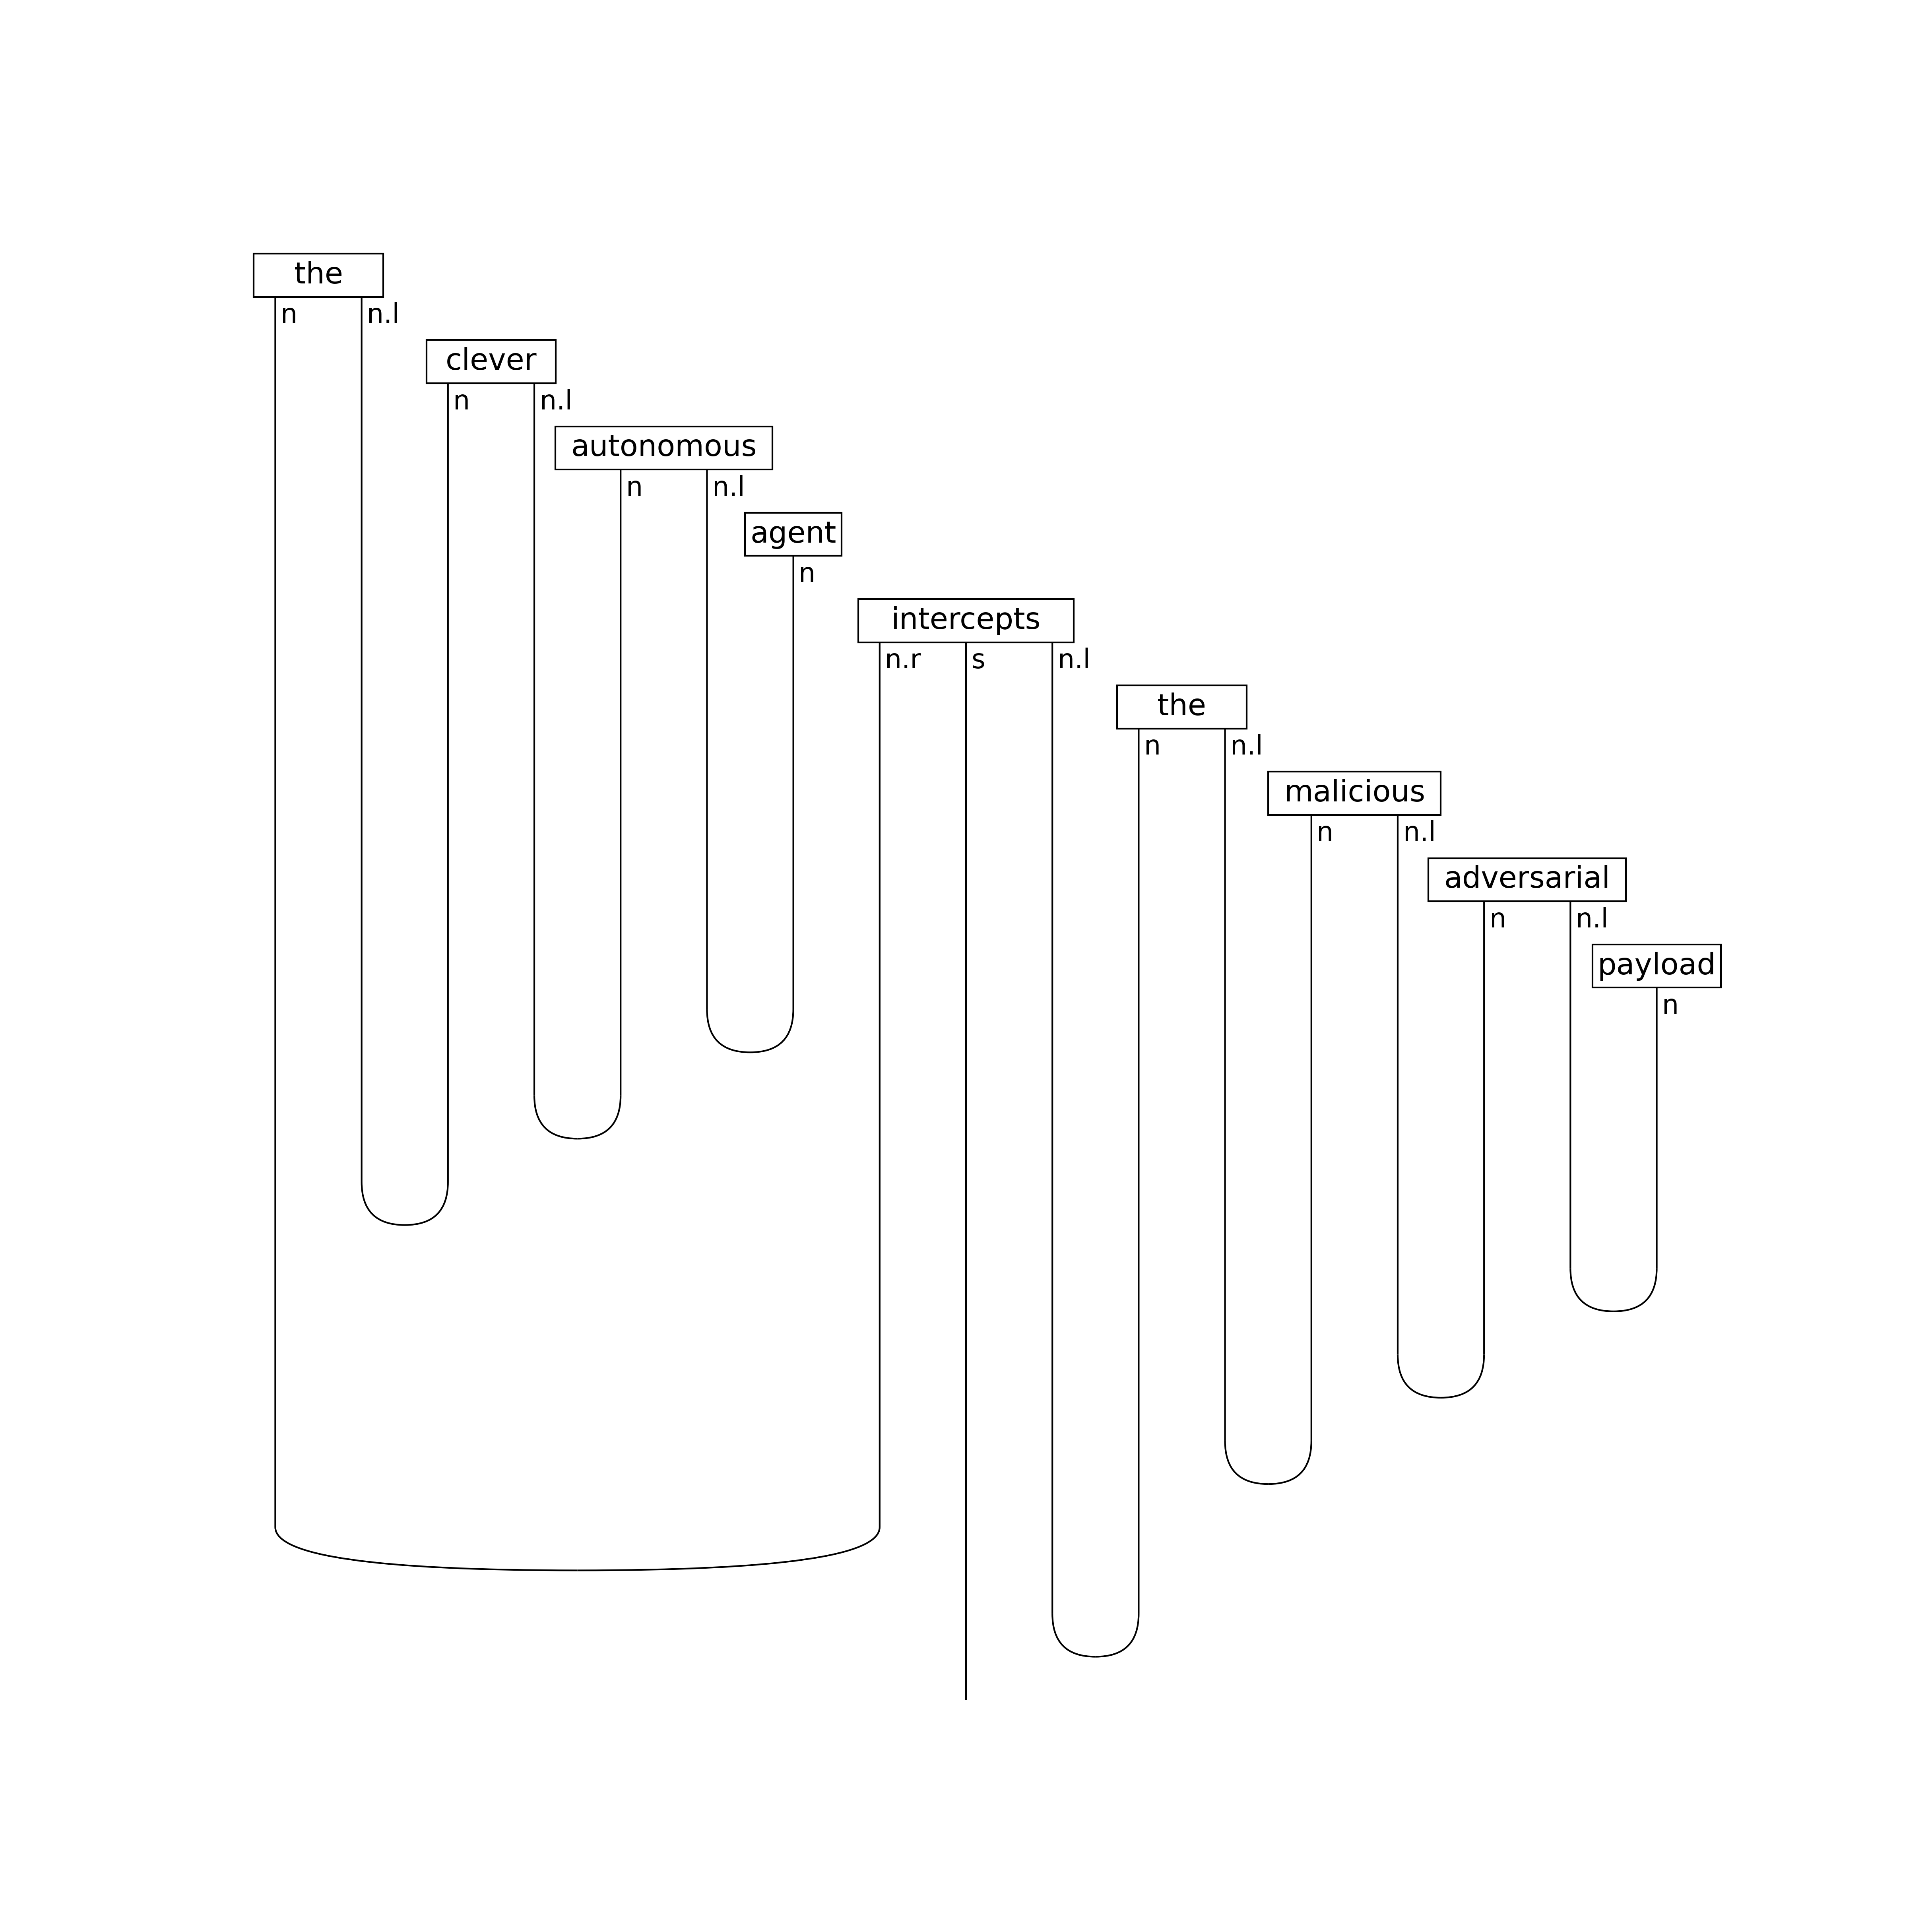
\includegraphics[keepaspectratio,alt={Direct DisCoPy machine output confirms pregroup type reduction to sentence wire s. Nine Word boxes carry complex noun-phrase types (e.g., n \textbackslash otimes n\^{}l for adjectives mapping an adjacent noun to a modified noun) and core verb types (n\^{}r \textbackslash otimes s \textbackslash otimes n\^{}l for the transitive ``intercepts''). Eight Cup contractions sequentially resolve the argument scopes from the deepest noun phrases outward, ultimately canceling all local adjoint pairs and reducing the extended initial tensor product to the single sentence wire s. Unlike the schematic progression in , this is the direct computational output of a multi-word discourse component, strictly confirming diagram.cod == s. By the Curry--Howard correspondence, this diagram simultaneously constitutes a syntactic derivation, a proof of well-typedness, and (under the meaning functor of ) a compositional semantic computation. Our extension decorates n-typed wires with functorial states S: \textbackslash mathbf\{Ent\} \textbackslash to \textbackslash mathbf\{Case\}, tracking role assignments across discourse boundaries via DisCoCirc entity wires.}]{../figures/discopy_transitive.png}}
\caption{Direct DisCoPy machine output confirms pregroup type reduction
to sentence wire \(s\). Nine Word boxes carry complex noun-phrase types
(e.g., \(n \otimes n^l\) for adjectives mapping an adjacent noun to a
modified noun) and core verb types (\(n^r \otimes s \otimes n^l\) for
the transitive ``intercepts''). Eight Cup contractions sequentially
resolve the argument scopes from the deepest noun phrases outward,
ultimately canceling all local adjoint pairs and reducing the extended
initial tensor product to the single sentence wire \(s\). Unlike the
schematic progression in \autoref{fig:string-diagram}, this is the
\emph{direct computational output} of a multi-word discourse component,
strictly confirming \protect\texttt{diagram.cod\ ==\ s}. By the
Curry--Howard correspondence, this diagram simultaneously constitutes a
syntactic derivation, a proof of well-typedness, and (under the meaning
functor of \autoref{sec:categorical-semantics}) a compositional semantic
computation. Our extension decorates \(n\)-typed wires with functorial
states \(S: \mathbf{Ent} \to \mathbf{Case}\), tracking role assignments
across discourse boundaries via \textbf{DisCoCirc entity
wires}.}\label{fig:discopy-transitive}
\end{figure}

For readers encountering pregroup reduction for the first time,
\autoref{fig:pregroup-unpacking} \emph{unpacks} the same construction
pedagogically: the four panels walk from the raw word types (panel 1),
through the parallel tensor that juxtaposes the boxes (panel 2), through
the application of the two cup contractions \(\varepsilon_n\) that
cancel each argument wire against its adjoint (panel 3), to the normal
form in which only the sentence wire \(s\) survives (panel 4). Each
panel is coloured by case role (NOM = blue, ACC = red, verb output in
indigo) so the identity of each wire is unambiguous.

\begin{figure}
\centering
\pandocbounded{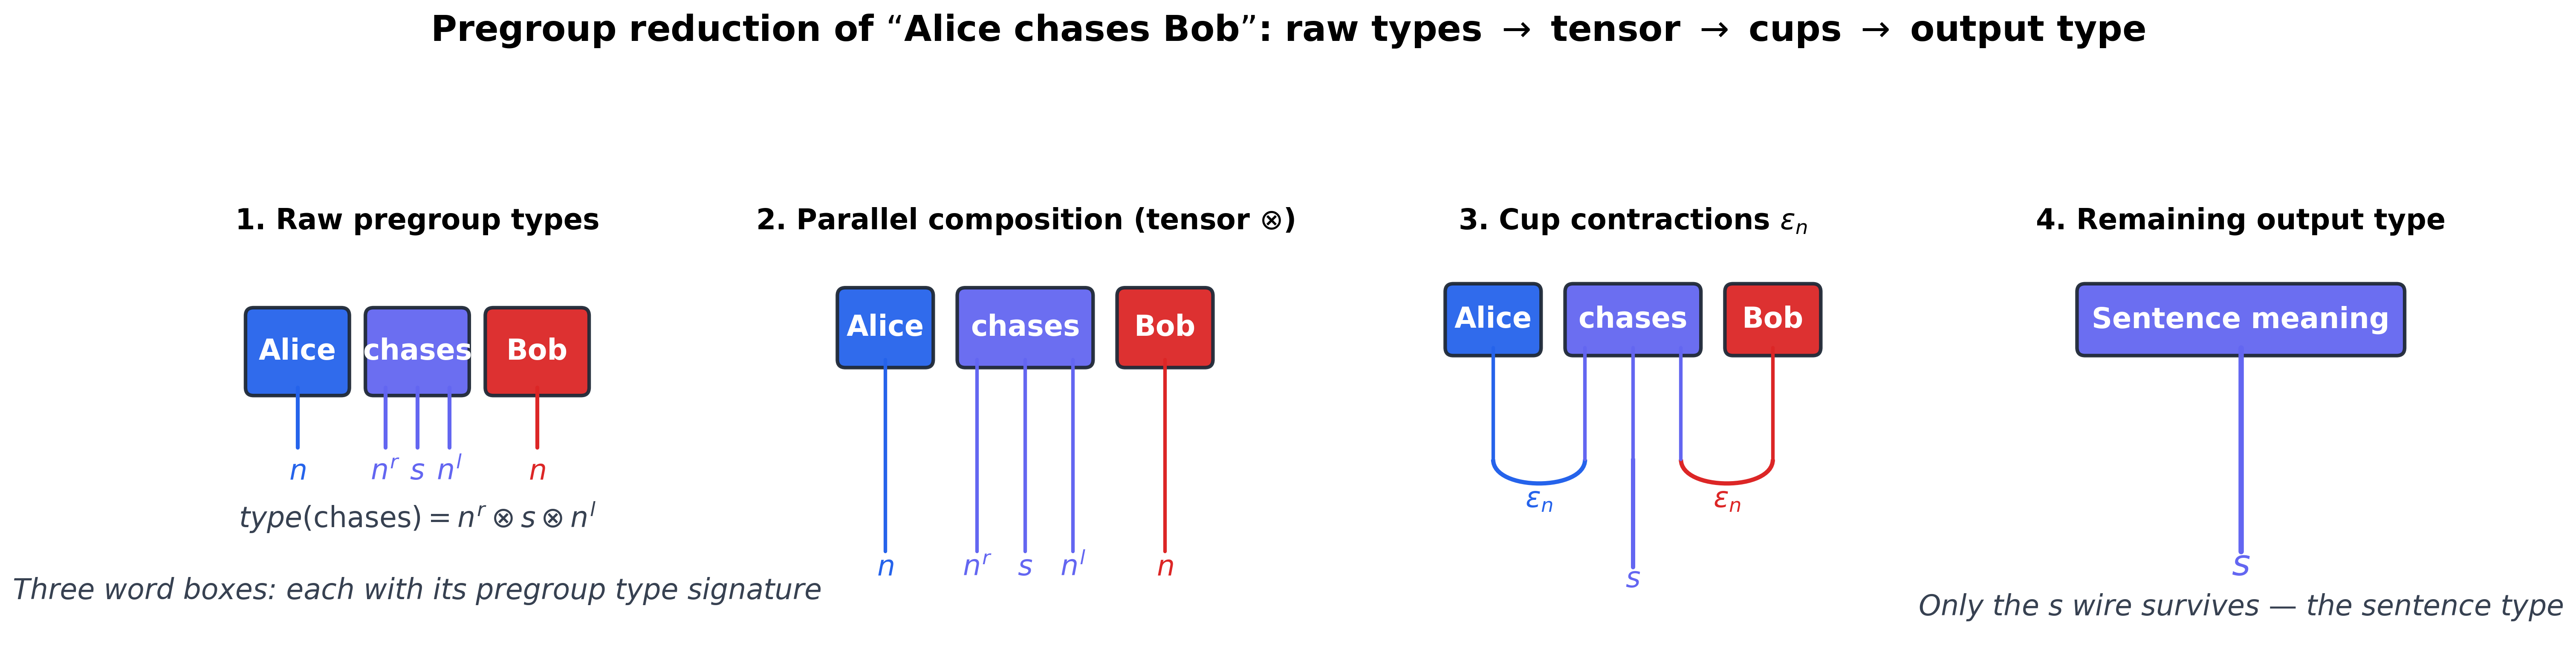
\includegraphics[keepaspectratio,alt={Pregroup reduction unpacked in four panels. Panel 1: raw pregroup types for Alice (n), chases (n\^{}r \textbackslash otimes s \textbackslash otimes n\^{}l), Bob (n). Panel 2: parallel composition \textbackslash otimes exposes all five dangling wires. Panel 3: the two cups \textbackslash varepsilon\_n cancel Alice's n against the verb's n\^{}r and the verb's n\^{}l against Bob's n, leaving only the central s wire. Panel 4: normal form --- the entire sentence reduces to a single s-typed wire. Generated programmatically from src.visualization.category\_unpacking.render\_pregroup\_reduction\_unpacking().}]{../figures/pregroup_reduction_unpacking.png}}
\caption{Pregroup reduction unpacked in four panels. Panel 1: raw
pregroup types for \emph{Alice} (\(n\)), \emph{chases}
(\(n^r \otimes s \otimes n^l\)), \emph{Bob} (\(n\)). Panel 2: parallel
composition \(\otimes\) exposes all five dangling wires. Panel 3: the
two cups \(\varepsilon_n\) cancel Alice's \(n\) against the verb's
\(n^r\) and the verb's \(n^l\) against Bob's \(n\), leaving only the
central \(s\) wire. Panel 4: normal form --- the entire sentence reduces
to a single \(s\)-typed wire. Generated programmatically from
\protect\texttt{src.visualization.category\_unpacking.render\_pregroup\_reduction\_unpacking()}.}\label{fig:pregroup-unpacking}
\end{figure}

\newpage

\section{Case Subscripts, Passivization, and the Curry--Howard
Proof}\label{sec:case-type-logic}

\textbf{Where we are in the argument.} \autoref{sec:categorial-grammar}
installed pregroup syntax --- cups, caps, and compact closure --- as the
algebraic backbone of composition. This chapter decorates that backbone
with case information: every noun wire picks up a case subscript
(\(n_{\text{NOM}}\), \(n_{\text{ACC}}\), \ldots) so grammatical role
becomes a first-class typed structure on wires, and passivization
becomes a wire-level swap together with \textbf{case relabeling}
(\autoref{eq:eq-3-3}/\autoref{eq:eq-3-4}) rather than an exception to
the type system --- the Curry--Howard image is a proof rewrite of that
rearrangement.

Case-marked noun phrases receive compound types that encode both their
grammatical role and their combinatory potential. For example, in a
nominative--accusative language, the type assignment proceeds as follows
(\autoref{tbl:pregroup-types}):

\begin{longtable}[]{@{}
  >{\raggedright\arraybackslash}p{(\linewidth - 4\tabcolsep) * \real{0.3333}}
  >{\raggedright\arraybackslash}p{(\linewidth - 4\tabcolsep) * \real{0.3333}}
  >{\raggedright\arraybackslash}p{(\linewidth - 4\tabcolsep) * \real{0.3333}}@{}}
\caption{Case-marked pregroup type assignments for a standard
nominative-accusative transitive
clause.}\label{tbl:pregroup-types}\tabularnewline
\toprule\noalign{}
\begin{minipage}[b]{\linewidth}\raggedright
Expression
\end{minipage} & \begin{minipage}[b]{\linewidth}\raggedright
Type
\end{minipage} & \begin{minipage}[b]{\linewidth}\raggedright
Gloss
\end{minipage} \\
\midrule\noalign{}
\endfirsthead
\toprule\noalign{}
\begin{minipage}[b]{\linewidth}\raggedright
Expression
\end{minipage} & \begin{minipage}[b]{\linewidth}\raggedright
Type
\end{minipage} & \begin{minipage}[b]{\linewidth}\raggedright
Gloss
\end{minipage} \\
\midrule\noalign{}
\endhead
\bottomrule\noalign{}
\endlastfoot
``Alice'' (subject) & \(n_{\text{NOM}}\) & Noun, nominative-marked \\
``the ball'' (object) & \(n_{\text{ACC}}\) & Noun, accusative-marked \\
``kicks'' & \((n_{\text{NOM}} \backslash s) / n_{\text{ACC}}\) & Seeks
ACC right, NOM left \\
``to Bob'' (recipient) & \((s \backslash s) / n_{\text{DAT}}\) &
Modifies sentence via DAT argument \\
\end{longtable}

The specific subscripts structurally refine the base noun type \(n\)
with mandatory continuous case features, mathematically guaranteeing
that the transitive verb ``kicks'' exclusively selects a
nominative-marked subject and an accusative-marked object. Any feature
mismatch automatically blocks the algebraic derivation, accurately
modeling native ungrammaticality.

\textbf{Alignment and natural transformations.} Cross-linguistic
alignment is modeled functorially in \autoref{sec:case-categories}:
alignment types are structure-preserving functors from a universal role
category to a language-specific case category, compared via natural
transformations when one asks how two alignments cohere on the same
underlying argument structure. At the level of case-marked pregroup
types (this section), that functorial picture \textbf{suggests} treating
agreement checks as naturality-style coherence constraints: the
morphosyntactic alignment chosen for arguments must remain compatible
with the verb's combinatorial requirements so that reductions still
factor through the intended case-typed slots. We do not claim a full
adjunction between identity and alignment functors in the pregroup
category here; the precise categorical status of alignment is anchored
in \autoref{sec:case-categories}, while the typed reductions below
supply the concrete syntax.

\subsection{Syntactic Derivation as Proof, Case Assignment as Type
Inference}\label{syntactic-derivation-as-proof-case-assignment-as-type-inference}

A deep structural parallel underlies the Lambek calculus: derivations of
syntactic types correspond to proofs in intuitionistic logic (via the
Curry--Howard isomorphism), and therefore to programs in a typed lambda
calculus, as summarized in \autoref{tbl:curry-howard}.

\begin{longtable}[]{@{}
  >{\raggedright\arraybackslash}p{(\linewidth - 4\tabcolsep) * \real{0.3333}}
  >{\raggedright\arraybackslash}p{(\linewidth - 4\tabcolsep) * \real{0.3333}}
  >{\raggedright\arraybackslash}p{(\linewidth - 4\tabcolsep) * \real{0.3333}}@{}}
\caption{The Curry--Howard isomorphism connecting syntactic, logical,
and computational domains.}\label{tbl:curry-howard}\tabularnewline
\toprule\noalign{}
\begin{minipage}[b]{\linewidth}\raggedright
Syntactic Domain
\end{minipage} & \begin{minipage}[b]{\linewidth}\raggedright
Logical Domain
\end{minipage} & \begin{minipage}[b]{\linewidth}\raggedright
Computational Domain
\end{minipage} \\
\midrule\noalign{}
\endfirsthead
\toprule\noalign{}
\begin{minipage}[b]{\linewidth}\raggedright
Syntactic Domain
\end{minipage} & \begin{minipage}[b]{\linewidth}\raggedright
Logical Domain
\end{minipage} & \begin{minipage}[b]{\linewidth}\raggedright
Computational Domain
\end{minipage} \\
\midrule\noalign{}
\endhead
\bottomrule\noalign{}
\endlastfoot
Types \((A / B, A \backslash B)\) & Propositions & Types \\
Derivations & Proofs & Programs (\(\lambda\text{-terms}\)) \\
Cut elimination & Proof normalization & \(\beta\text{-reduction}\) \\
Commutativity of cuts & Confluence of rewriting & Church--Rosser
property \\
\end{longtable}

This foundational correspondence dictates two critical consequences for
our cognitive framework:

\begin{enumerate}
\def\labelenumi{\arabic{enumi}.}
\tightlist
\item
  \textbf{Semantic compositionality strictly follows syntactic
  well-formedness}: A successfully typed derivation automatically
  guarantees a well-formed geometric meaning representation
  (specifically, the exact \(\lambda\text{-term}\) isolated and
  extracted directly from the formal proof).
\item
  \textbf{Case assignment reduces to type inference}: Dynamically
  determining the correct case for a noun phrase in context is
  computationally equivalent to inferring the type of an unknown
  variable in a \(\lambda\text{-expression}\)---thereby grounding case
  assignment in the well-understood algorithmic landscape of type
  inference (Hindley-Milner and its extensions).
\end{enumerate}

\subsection{Song's Monadic Root Syntax: Sublexical Decomposition via
Embedded
Monads}\label{songs-monadic-root-syntax-sublexical-decomposition-via-embedded-monads}

Song \citetext{\citeyear{song2022act}; \citeyear{song2022blog}}
significantly extends this categorial framework by deploying a novel
\textbf{monadic semantics} for root syntax. He successfully models the
sublexical decomposition of complex verb roots by embedding specialized
monads directly into the base syntactic category. This computational
approach captures the deep intuition that a seemingly simple verb like
``break'' harbors layered internal structure---specifically, an active
causative layer tightly coupled to a passive result-state layer---which
dynamically dictates subsequent case assignment. The formal monad
elegantly encapsulates this tangled lexical complexity within one
streamlined categorical construction, empowering the type-logical
grammar to process lexical features and syntactic composition
simultaneously and uniformly.

This monadic architecture seamlessly interfaces with modern graded type
theory. For instance, Asudeh and Giorgolo \citeyearpar{asudeh2020graded}
previously developed a monadic semantics tracking evidentiality,
deploying graded computational effects to quantify the shifting
epistemic real-world status of various propositions. Our framework
extends this exact pattern into the domain of morphological case, where
the continuous ``grade'' attached to any specific morphism formally
encodes the statistical strength and validity of that local semantic
role assignment.

\subsection{Passivization Is a Swap: Voice Alternation as Topological
Wire
Crossing}\label{passivization-is-a-swap-voice-alternation-as-topological-wire-crossing}

Within categorical linguistics, \textbf{passivization} emerges as a
uniquely revealing topological operation. Traditionally described as a
syntactic rule that promotes the patient to subject position while
(optionally) demoting the agent to an oblique role, passivization in our
framework ceases to be an ad-hoc transformation; instead, it combines
(i) a \textbf{Swap} morphism
\(\sigma_{A,B}: A \otimes B \to B \otimes A\) that crosses the noun
wires feeding into the verb's pregroup derivation---so \emph{which} noun
meets the verb's left vs.~right adjoint slots reverses relative to the
active diagram---and (ii) \textbf{updated case features} on those wires:
the promoted subject is \(n_{\text{NOM}}\), not a carried-over
\(n_{\text{ACC}}\).

In a pregroup grammar, the active transitive ``Alice chases Bob'' has
the type reduction:

\begin{equation}
n_{\text{NOM}} \cdot (n^r \cdot s \cdot n^l) \cdot n_{\text{ACC}} \to s
\label{eq:eq-3-3}
\end{equation}

For ``Bob is chased by Alice,'' Bob is the grammatical subject
(\(n_{\text{NOM}}\)) and Alice appears in the oblique \emph{by}-phrase
(\(n_{\text{OBL}}\)), with surface order subject--verb--oblique:

\begin{equation}
n_{\text{NOM}} \cdot (n^r \cdot s \cdot n^l) \cdot n_{\text{OBL}} \to s
\label{eq:eq-3-4}
\end{equation}

This is \textbf{not} the naive swap of subscripts in \eqref{eq:eq-3-3}
(which would incorrectly leave the promoted patient typed as
accusative). The DisCoPy \texttt{Swap} primitive makes the wire crossing
explicit; the case-marked types in \eqref{eq:eq-3-4} match the figure
and standard promotion/demotion. The generated passive diagram diverges
from its active counterpart through that crossing together with the
reassignment of which noun occupies each cup. This transforms abstract
syntactic voice alternation into a highly visible, instantly readable
topological feature embedded directly within the string diagram.

This diagrammatic transparency exemplifies Shimojima's
\citeyearpar{shimojima1996reasoning} free-ride inference capability. By
inspecting the visual topology, a cognitive agent immediately verifies
that passivization preserves the verb's inherent argument structure
while rearranging its surface realization---a structural fact that
typically requires chaining inference steps to algebraically establish
within standard linear notation (\autoref{fig:discopy-passive}).

\begin{figure}
\centering
\pandocbounded{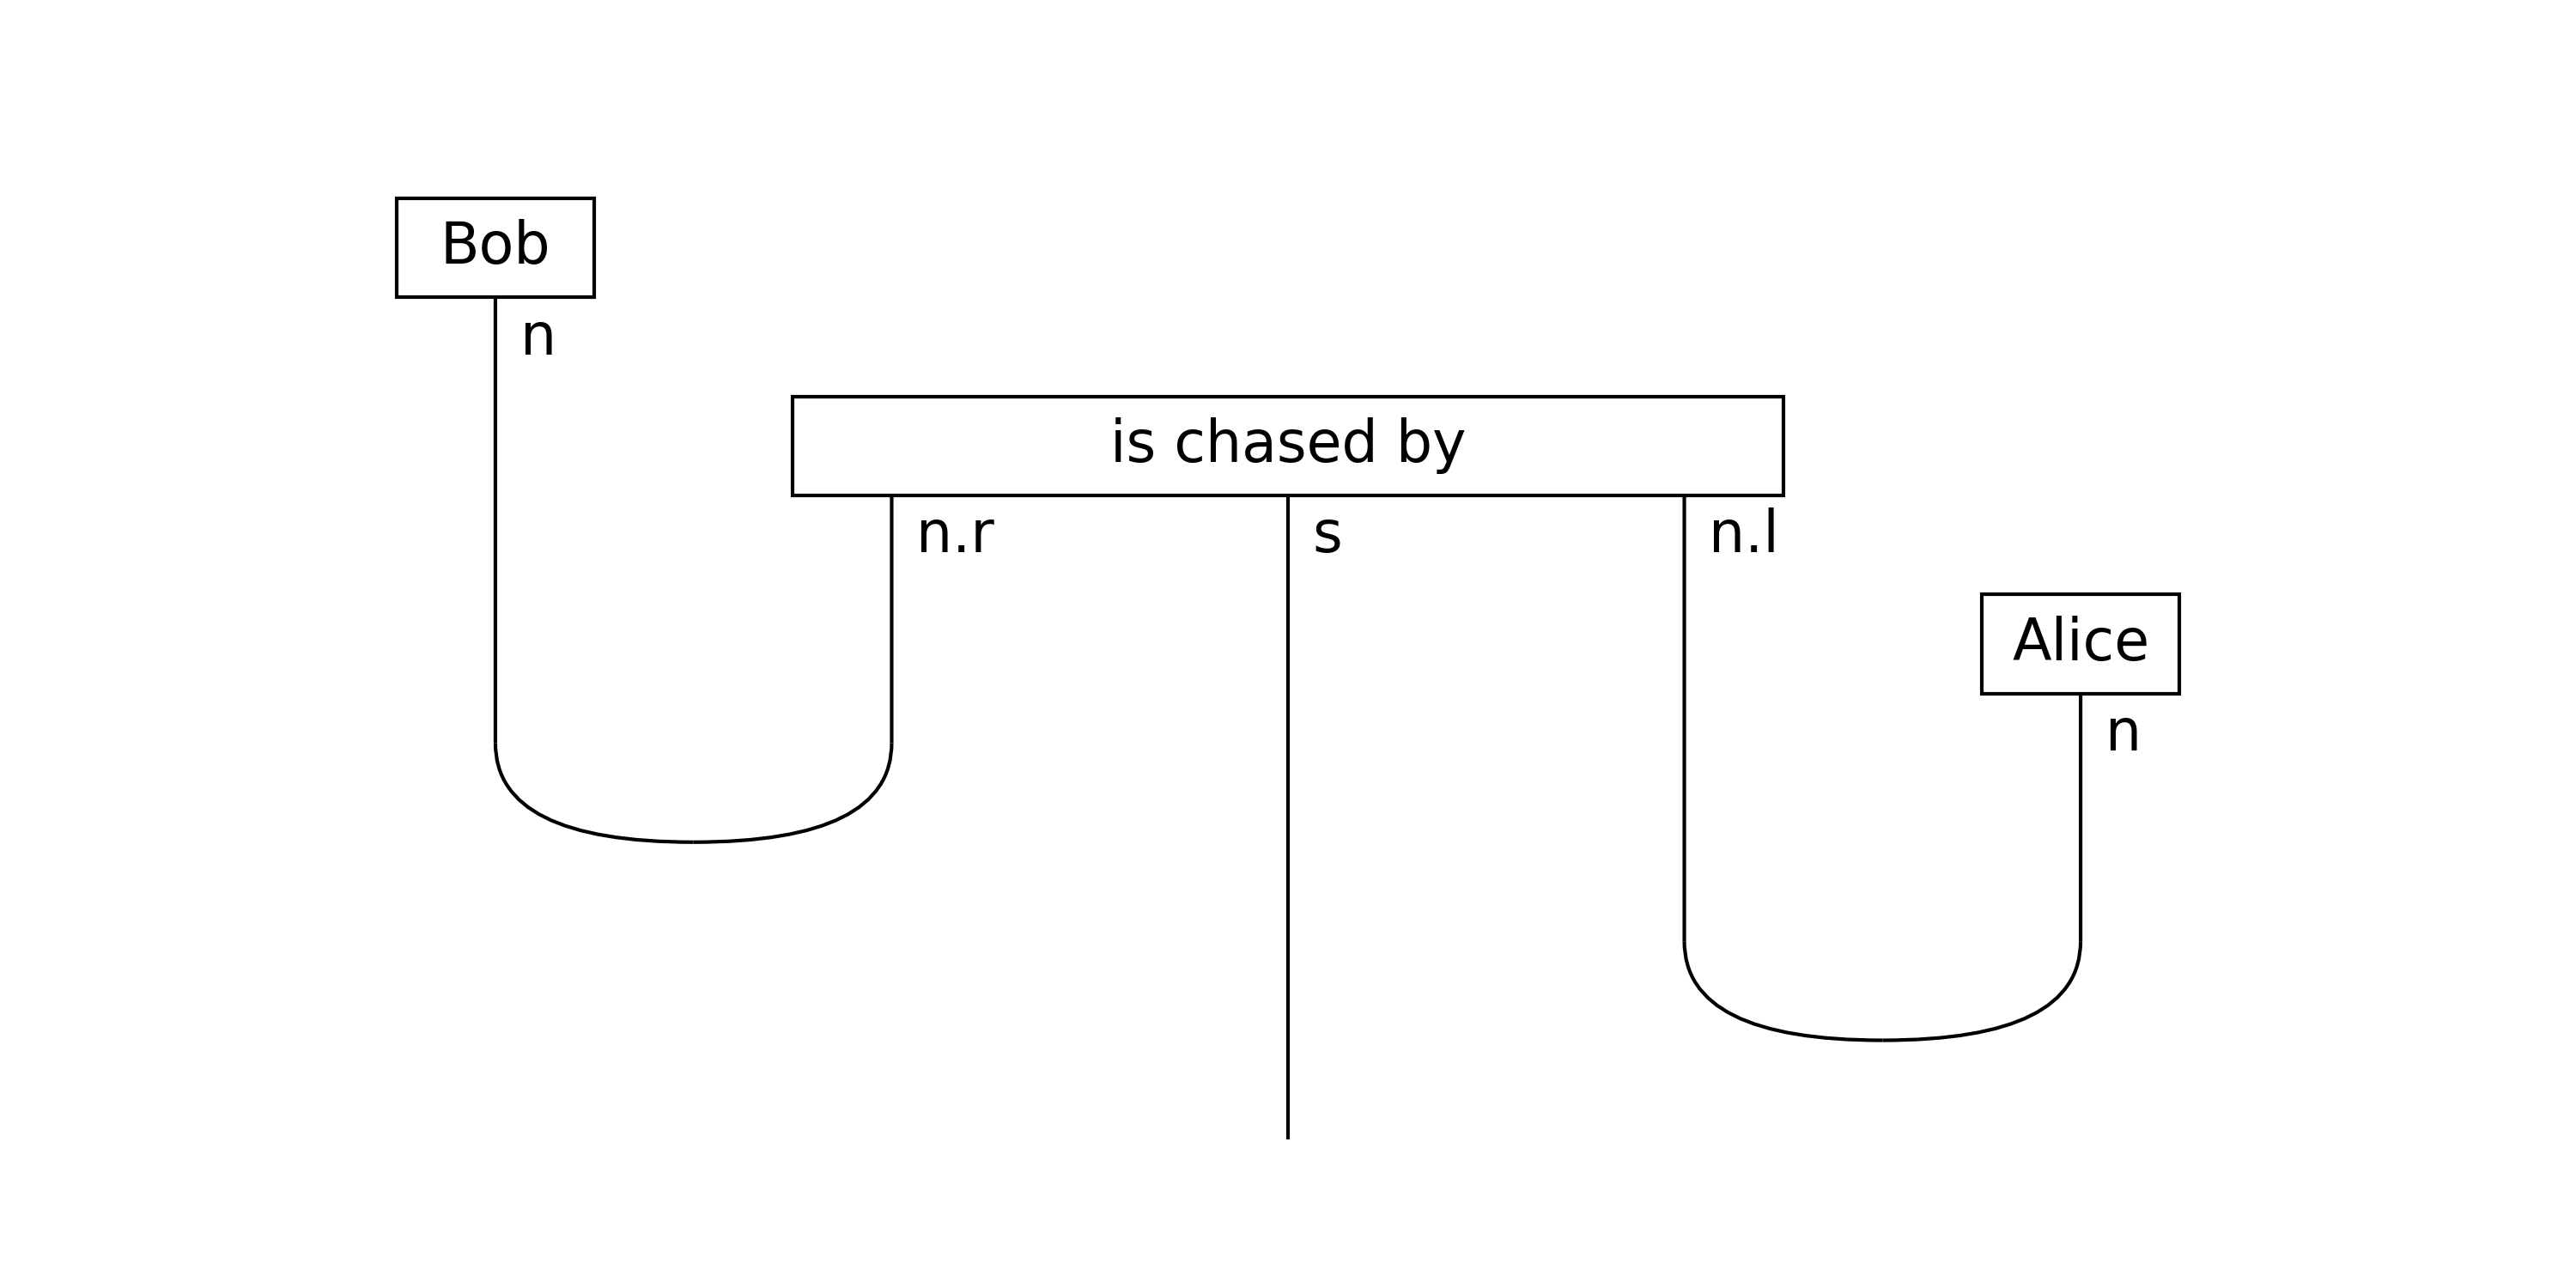
\includegraphics[keepaspectratio,alt={Passivization as role reassignment in the DisCoPy pregroup diagram for ``Bob is chased by Alice'' with type n\_\{\textbackslash text\{NOM\}\} \textbackslash otimes (n\^{}r \textbackslash otimes s \textbackslash otimes n\^{}l) \textbackslash otimes n\_\{\textbackslash text\{OBL\}\} \textbackslash to s. Bob's n wire contracts into the verb's left adjoint n\^{}r via the left Cup (n--n\^{}r) --- promoting the semantic patient to grammatical subject --- while Alice's n wire contracts into the right adjoint n\^{}l via the right Cup (n\^{}l--n), now demoted to the oblique by-phrase. Compare with  (active ``Alice chases Bob''), where Alice occupies the left subject slot and Bob the right object slot: the reassignment of which noun lands in each Cup is what makes voice alternation a topological swap \textbackslash sigma\_\{n,n\}\textbackslash colon n \textbackslash otimes n \textbackslash to n \textbackslash otimes n rather than a lexical substitution. Cup count is unchanged (two, matching the transitive active), so \textbackslash kappa(D) tracks argument slots rather than surface case marking; per  only the box count distinguishes the two diagrams (the passive inserts the ``is chased by'' box in place of the active ``chases'' box).}]{../figures/discopy_passive.png}}
\caption{Passivization as role reassignment in the DisCoPy pregroup
diagram for ``Bob is chased by Alice'' with type
\(n_{\text{NOM}} \otimes (n^r \otimes s \otimes n^l) \otimes n_{\text{OBL}} \to s\).
Bob's \(n\) wire contracts into the verb's left adjoint \(n^r\) via the
left Cup (\(n\)--\(n^r\)) --- promoting the semantic patient to
grammatical subject --- while Alice's \(n\) wire contracts into the
right adjoint \(n^l\) via the right Cup (\(n^l\)--\(n\)), now demoted to
the oblique \emph{by}-phrase. Compare with
\autoref{fig:discopy-discocat} (active ``Alice chases Bob''), where
Alice occupies the left subject slot and Bob the right object slot: the
reassignment of \emph{which} noun lands in each Cup is what makes voice
alternation a topological swap
\(\sigma_{n,n}\colon n \otimes n \to n \otimes n\) rather than a lexical
substitution. Cup count is unchanged (two, matching the transitive
active), so \(\kappa(D)\) tracks argument slots rather than surface case
marking; per \autoref{eq:eq-4-4} only the box count distinguishes the
two diagrams (the passive inserts the ``is chased by'' box in place of
the active ``chases'' box).}\label{fig:discopy-passive}
\end{figure}

Relative to \autoref{eq:eq-4-4}, the passive ``Bob is chased by Alice''
diagram in \autoref{fig:discopy-passive} has the same cup count as the
transitive active and therefore nearly identical \(\kappa(D)\); the
syntactic reassignment is visible in \emph{which} cup each noun enters,
not in the total count of contractions.

\newpage

\section{Categorical Distributional Semantics (DisCoCat): Composing
Vector Spaces via Type Derivations}\label{sec:categorical-semantics}

\textbf{Where we are in the argument.}
\autoref{sec:categorial-grammar}--\autoref{sec:case-type-logic} gave the
framework a \emph{syntactic} apparatus: pregroup derivations with
case-typed wires. This chapter supplies the matching \emph{semantic} one
--- the Coecke--Sadrzadeh--Clark meaning functor
\(F \colon \mathbf{Preg} \to \mathbf{FinHilb}\) that sends each word to
a tensor in a vector space and each pregroup contraction to an
inner-product composition, so the same syntactic diagram simultaneously
proves well-typedness \emph{and} computes the composed meaning.

\subsection{The Formalism--Distribution Impasse and Why Montague Cannot
Meet
Harris}\label{the-formalismdistribution-impasse-and-why-montague-cannot-meet-harris}

The study of linguistic meaning has historically been fractured between
two traditions offering complementary strengths and weaknesses:

\begin{enumerate}
\def\labelenumi{\arabic{enumi}.}
\item
  \textbf{Formal semantics}, following Montague
  \citeyearpar{montague1973proper}, strictly models meaning
  compositionally: the algebraic meaning of any complex expression
  functions as a direct product of its parts and their syntactic
  combination. This tradition excels at capturing rigid logical
  structure (quantification, negation, modality) but severely struggles
  with fluid lexical meaning, typically treating content words as
  opaque, unanalyzed primitives.
\item
  \textbf{Distributional semantics} models meaning empirically: a word's
  meaning organically emerges from its distribution across contexts,
  typically encoded computationally as a dense vector in
  high-dimensional space. This distributional hypothesis---famously
  summarized as ``You shall know a word by the company it keeps''
  \citep{firth1957papers}---traces directly to J.R. Firth and Zellig
  Harris \citeyearpar{harris1954distributional}, whose algebraic
  analysis proved that linguistic elements occurring in similar
  environments inherently share semantic properties. While this
  tradition beautifully captures graded similarity and geometric
  analogy, it lacks rigorous compositional structure. Under pure
  distribution, ``dog bites man'' and ``man bites dog'' collapse into
  identical vector representations.
\end{enumerate}

This theoretical tension represents one of the deepest impasses in
modern cognitive science. Turney and Pantel's
\citeyearpar{turney2010frequency} survey of vector space models proved
that distributional methods capture fine-grained semantic
distinctions---synonymy, antonymy, hypernymy, analogy---but isolate
these victories to the word level. Baroni and Lenci
\citeyearpar{baroni2010distributional} built a tensor-based
\emph{Distributional Memory} framework partially addressing this
compositionality by structuring co-occurrence data into a three-way
tensor over (word, relation, word) triples, yet this approach lacked a
principled type-logical backbone. Lenci
\citeyearpar{lenci2018distributional} surveyed this landscape and
identified the central open problem: how to fuse the \emph{algebraic
compositionality} of formal semantics with the \emph{empirical
grounding} of distributional vector models.

The \textbf{DisCoCat} (Distributional Compositional Categorical)
framework \citep{coecke2010mathematical} resolves this long-standing
tension. It deploys category theory to compose distributional meanings
directly according to syntactic structure, yielding a semantic framework
that is simultaneously \emph{compositional} (via categorial grammar),
\emph{distributional} (via corpus-derived vector spaces), and
\emph{algebraically principled} (via rigid monoidal category theory).

\subsection{From Word2Vec to Transformer Attention: DisCoCat as the
Algebraic Formalization of Distributional
Semantics}\label{from-word2vec-to-transformer-attention-discocat-as-the-algebraic-formalization-of-distributional-semantics}

The distributional programme has undergone a dramatic computational
intensification in the era of large language models (LLMs). The
trajectory from classical co-occurrence matrices through static word
embeddings to contextual transformers can be understood as a progressive
\emph{enrichment} of the distributional hypothesis itself:

\begin{enumerate}
\def\labelenumi{\arabic{enumi}.}
\item
  \textbf{Static embeddings}: Mikolov et al.'s
  \citeyearpar{mikolov2013efficient} Word2Vec (skip-gram and CBOW)
  demonstrated that targeted prediction-based training on local context
  windows naturally generates word vectors exhibiting striking algebraic
  regularity---yielding the famous ``king \(-\) man \(+\) woman
  \(\\approx\) queen'' geometric analogy. Pennington et al.'s
  \citeyearpar{pennington2014glove} GloVe successfully incorporated
  global co-occurrence statistics via log-bilinear regression, yielding
  dense vectors whose inner products cleanly approximate underlying
  pointwise mutual information. Both models instantiate the
  distributional hypothesis in its classical Firthian form: contextual
  use strictly determines meaning, permanently encoding it as geometric
  position within a learned vector space.
\item
  \textbf{Contextual embeddings}: BERT \citep{devlin2019bert} and GPT
  \citep{radford2018improving} dramatically push beyond static
  type-level representations into dynamic \emph{token-level}
  contextualized embeddings, where the identical word dynamically
  receives entirely different coordinate vectors in varying contexts. In
  terms of the formal vs.~distributional dichotomy, this jump represents
  a critical advance: contextualized embeddings successfully (though
  implicitly) capture \emph{compositional} structure by continuously
  conditioning word representations upon their full sentential
  environment. This addresses polysemy and complex constructional
  effects that static embeddings routinely conflate.
\item
  \textbf{Transformer architecture}: The transformer
  \citep{vaswani2017attention} implements distributional composition via
  multi-head self-attention, where each head computes a weighted
  combination of input token representations. The attention weights
  \(\alpha_{ij} = \mathrm{softmax}(Q_i K_j^T / \sqrt{d_k})\) operate
  analogously to the enriched hom-values detailed in
  \autoref{sec:enriched-categories}: they encode the \emph{degree of
  contextual relevance} between tokens \(i\) and \(j\) within a tuned
  representational subspace---yielding a graded, learned distributional
  mapping.
\end{enumerate}

The mapping back to our categorical framework is direct:
\textbf{DisCoCat supplies the algebraic formalization of what modern
LLMs learn empirically.} A transformer builds sentence representations
by attending to syntactically and semantically relevant tokens through
learned weight matrices. DisCoCat achieves the same goal by composing
word vectors through type-logical derivations within a compact closed
category. The central functor \(F: \mathbf{Preg} \to \mathbf{FVect}\)
defining DisCoCat is therefore the \emph{principled} version of the
composition that neural attention learns from data. Gavranović's
\citeyearpar{gavranovic2024thesis} categorical learning programme
confirms this perspective rigorously, proving that neural attention
heads operate as parameterized optics---categorical constructions
composing functorially, mirroring DisCoCat derivations.

For case theory specifically, the transformer analogy is illuminating:
each attention head in a transformer can be understood as learning a
particular \emph{relational role}---attending to subjects, objects,
modifiers, or other grammatical functions. This is precisely the role
that case marking plays in natural language: structuring
who-does-what-to-whom. The case-typed noun spaces of our enriched
DisCoCat model
(\(N_{\text{NOM}}, N_{\text{ACC}}, N_{\text{DAT}}, \ldots\)) correspond
to the role-specific representational subspaces that different attention
heads learn to inhabit.

\subsection{\texorpdfstring{The Meaning Functor
\(F: \mathbf{Preg} \to \mathbf{FVect}\)}{The Meaning Functor F: \textbackslash mathbf\{Preg\} \textbackslash to \textbackslash mathbf\{FVect\}}}\label{sec:discocat-meaning-functor}

\subsubsection{Pregroups and Vector Spaces Share a
Category}\label{pregroups-and-vector-spaces-share-a-category}

DisCoCat's central observation is that pregroup grammars and vector
spaces share a common abstract structure: both are \textbf{compact
closed categories}. This means there exists a \emph{meaning functor}:

\begin{equation}
F: \mathbf{Preg} \to \mathbf{FVect}
\label{eq:eq-4-1}
\end{equation}

from the pregroup grammar category (where objects are types and
morphisms are grammatical reductions) to the category of
finite-dimensional vector spaces (where objects are vector spaces and
morphisms are linear maps).

Under this functor:

\begin{itemize}
\tightlist
\item
  Noun types \(n\) map to a vector space \(N\) (the noun space)
\item
  Sentence types \(s\) map to a vector space \(S\) (the sentence space)
\item
  A transitive verb of type \(n^r \cdot s \cdot n^l\) maps to a tensor
  in \(N \otimes S \otimes N\)
\item
  Pregroup contractions (cups/caps) map to the standard inner product
  and its dual
\end{itemize}

\subsubsection{Tensoring, Then Contracting: How ``Alice Chases Bob''
Becomes a
Vector}\label{tensoring-then-contracting-how-alice-chases-bob-becomes-a-vector}

The compositional meaning of a sentence is computed by tensoring the
word meanings and then contracting the result along the indices
determined by the syntactic derivation. For ``Alice chases Bob'':

\begin{equation}
\overrightarrow{\text{Alice chases Bob}} = (\overrightarrow{\text{Alice}} \otimes \overleftrightarrow{\text{chases}} \otimes \overrightarrow{\text{Bob}}) \circ (\varepsilon_N \otimes 1_S \otimes \varepsilon_N)
\label{eq:eq-4-2}
\end{equation}

where \(\varepsilon_N: N \otimes N \to \mathbb{R}\) is the compact
closure map (inner product). This computation has a direct diagrammatic
representation as a string diagram---the same Joyal--Street
\citep{joyalstreet1991geometry} formalism that governs the syntax.

\subsubsection{DisCoCat Resolves ``Dog Bites Man'' vs ``Man Bites
Dog''}\label{discocat-resolves-dog-bites-man-vs-man-bites-dog}

Grefenstette and Sadrzadeh \citeyearpar{grefenstette2015concrete}
demonstrated that DisCoCat models can outperform purely distributional
baselines on disambiguation and sentence similarity tasks. The key
advantage is that compositional structure resolves ambiguities that
bag-of-words models cannot: ``dog bites man'' and ``man bites dog''
receive different sentence vectors because the syntactic structure
assigns different roles to the nouns.

\textbf{Attention as Cup contraction.} The claim that DisCoCat provides
the ``algebraic formalization'' of transformer-based LLMs can be made
precise. In a transformer's self-attention mechanism, the query--key
inner product \(\mathrm{softmax}(QK^\top / \sqrt{d})V\) selects which
word vectors interact---effectively implementing a \emph{soft} version
of the Cup contraction. The pregroup Cup
\(\varepsilon: n^r \otimes n \to I\) contracts two noun wires into a
scalar; the attention inner product \(q_i \cdot k_j\) contracts two
contextualized vectors into an attention weight, which then mixes the
value vectors. The difference is that the DisCoCat Cup is \emph{binary}
(either the types match or they don't) while the attention Cup is
\emph{graded} (producing a real-valued weight). This is precisely the
\([0,1]\)-enrichment of \autoref{sec:enriched-categories} applied to the
type-reduction level: each attention head learns an enriched Cup that
contracts types with learned confidence weights rather than categorical
yes/no type-matching. Multi-head attention then corresponds to the
tensor product of \(h\) independent enriched contraction maps, each
attending to a different substring of the relational
structure---analogous to how DisCoCat composes multiple Cup contractions
for multi-argument verbs (\autoref{fig:discopy-discocat}).

\begin{figure}
\centering
\pandocbounded{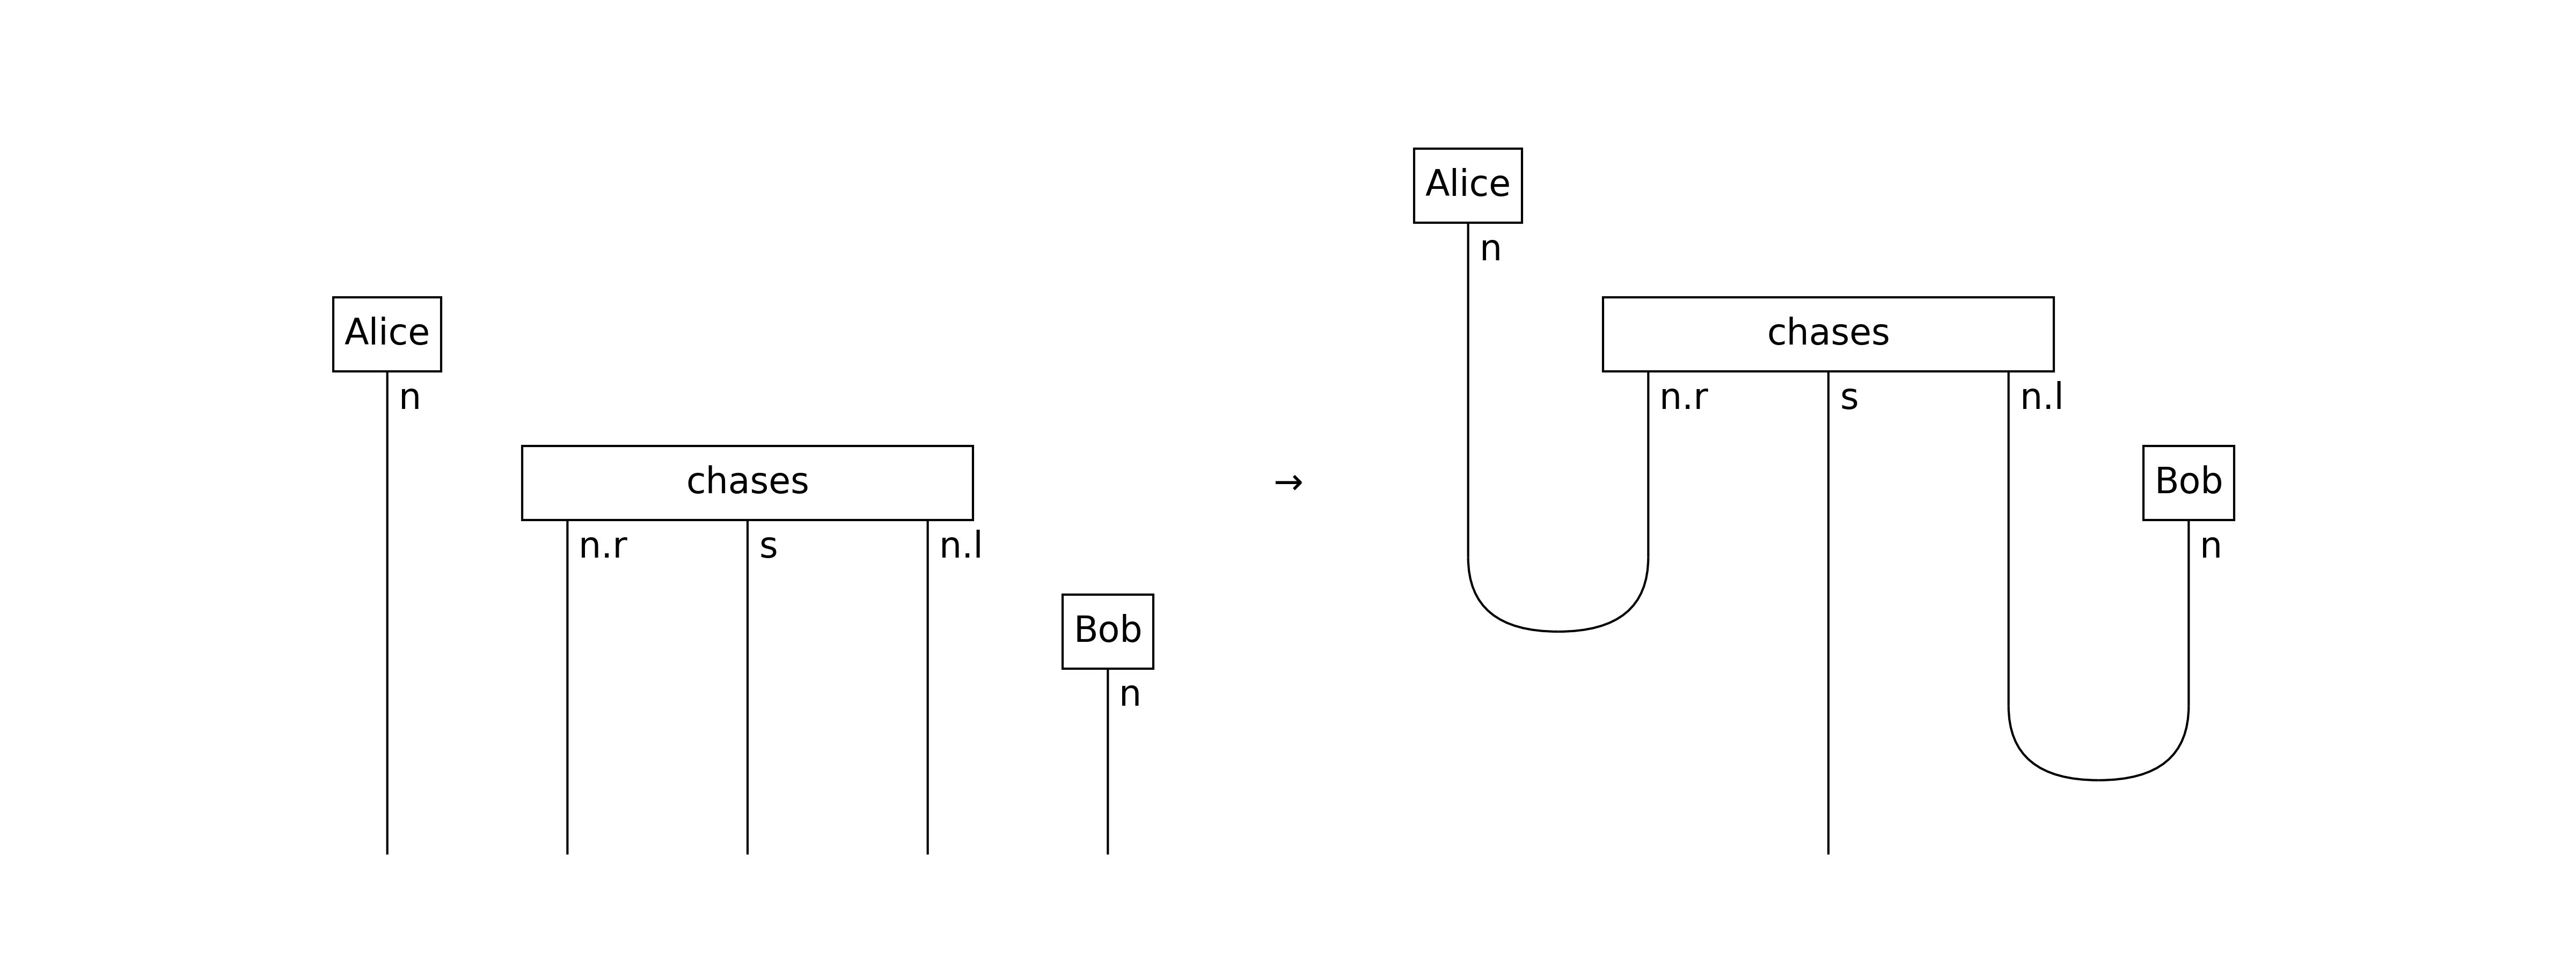
\includegraphics[keepaspectratio,alt={Cup contractions compute sentence meaning by contracting word tensors along syntactically determined indices. The DisCoCat meaning functor F: \textbackslash mathbf\{Preg\} \textbackslash to \textbackslash mathbf\{FVect\} applied to ``Alice chases Bob.'' Left panel: pre-contraction tensor product n \textbackslash otimes (n\^{}r \textbackslash otimes s \textbackslash otimes n\^{}l) \textbackslash otimes n, showing three Word boxes with pregroup types. Right panel: fully contracted diagram where two Cup contractions (\textbackslash varepsilon: n\^{}r \textbackslash otimes n \textbackslash to 1 and \textbackslash varepsilon: n\^{}l \textbackslash otimes n \textbackslash to 1) reduce the five-wire product to sentence wire s. Under F, noun types map to N, the sentence type to S, and the verb's type to \textbackslash overleftrightarrow\{\textbackslash text\{chases\}\} \textbackslash in N \textbackslash otimes S \textbackslash otimes N. The Cup contractions become inner products \textbackslash varepsilon\_N: N \textbackslash otimes N \textbackslash to \textbackslash mathbb\{R\}, computing \textbackslash overrightarrow\{\textbackslash text\{Alice chases Bob\}\} \textbackslash in S.}]{../figures/discopy_composition.png}}
\caption{Cup contractions compute sentence meaning by contracting word
tensors along syntactically determined indices. The DisCoCat meaning
functor \(F: \mathbf{Preg} \to \mathbf{FVect}\) applied to ``Alice
chases Bob.'' \textbf{Left panel}: pre-contraction tensor product
\(n \otimes (n^r \otimes s \otimes n^l) \otimes n\), showing three Word
boxes with pregroup types. \textbf{Right panel}: fully contracted
diagram where two Cup contractions (\(\varepsilon: n^r \otimes n \to 1\)
and \(\varepsilon: n^l \otimes n \to 1\)) reduce the five-wire product
to sentence wire \(s\). Under \(F\), noun types map to \(N\), the
sentence type to \(S\), and the verb's type to
\(\overleftrightarrow{\text{chases}} \in N \otimes S \otimes N\). The
Cup contractions become inner products
\(\varepsilon_N: N \otimes N \to \mathbb{R}\), computing
\(\overrightarrow{\text{Alice chases Bob}} \in S\).}\label{fig:discopy-discocat}
\end{figure}

\subsection{Case-Typed Noun Spaces and Alignment as Natural
Transformation}\label{case-typed-noun-spaces-and-alignment-as-natural-transformation}

The present contribution lies in showing how case marking enriches the
DisCoCat framework with explicit role structure. In a case-marked
DisCoCat model:

\begin{enumerate}
\def\labelenumi{\arabic{enumi}.}
\item
  \textbf{Typed noun spaces}: Instead of a single noun space \(N\), we
  define case-specific spaces
  \(N_{\text{NOM}}, N_{\text{ACC}}, N_{\text{DAT}}, \ldots\) Morphisms
  between these spaces encode case-changing operations (passivization,
  dative shift, etc.).
\item
  \textbf{Case-constrained composition}: The meaning functor \(F\) maps
  case-typed pregroup derivations to tensor contractions that respect
  case constraints. A verb seeking a nominative subject and accusative
  object contracts only with vectors from the appropriate spaces.
\item
  \textbf{Alignment as Natural Transformation}: Cross-linguistic
  alignment differences correspond to different meaning functors.
  However, we go further by modeling case alignment as \textbf{natural
  transformations} between functors. An accusative-language
  transformation \(\nu_{\text{acc}}: \mathcal{I} \to F_{\text{acc}}\)
  identifies S and A arguments; an ergative transformation
  \(\nu_{\text{erg}}\) identifies S and P. (We write \(\nu\) here so
  \(\eta{}\) remains reserved for the compact-closure \textbf{cap} in
  pregroup diagrams.) This categorification allows us to model
  ``grammar'' as the requirement that these transformations commute with
  the DisCoCirc entity wires, ensuring role persistence across
  sentences.
\end{enumerate}

\begin{figure}
\centering
\pandocbounded{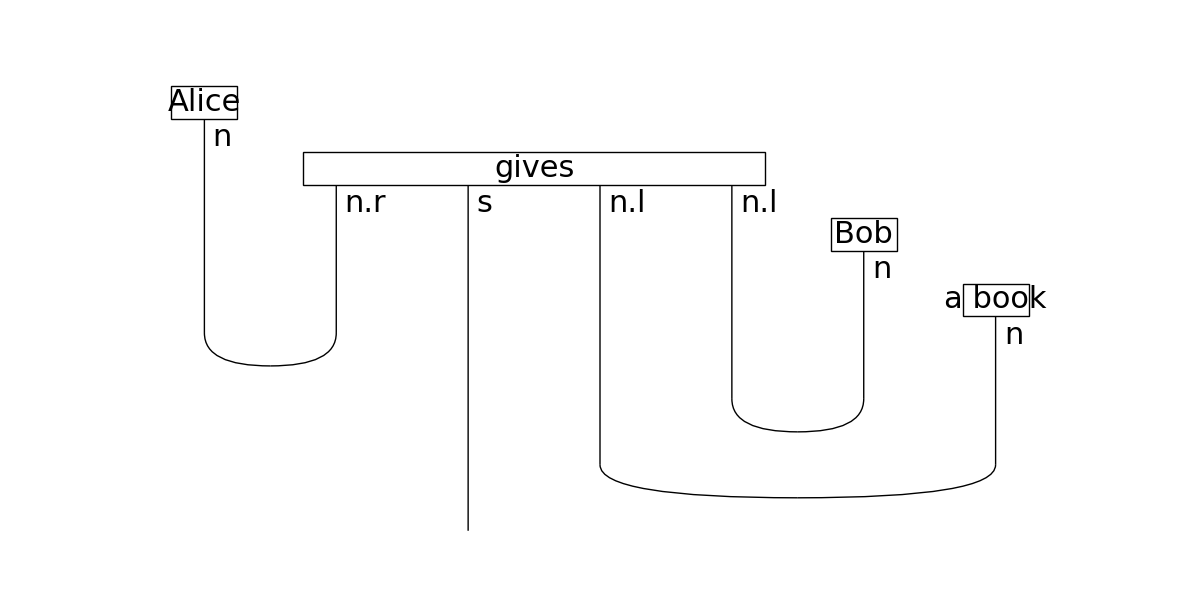
\includegraphics[keepaspectratio,alt={Ditransitive pregroup diagram for ``Alice gives Bob a book'': four word boxes (Alice, gives, Bob, book) with three Cup contractions reducing the five-argument tensor to sentence type s, exhibiting higher valency (\textbackslash kappa(D)) than a transitive clause. Generated by render\_discopy\_ditransitive() in src/visualization/discopy\_diagrams.py.}]{../figures/discopy_ditransitive.png}}
\caption{Ditransitive pregroup diagram for ``Alice gives Bob a book'':
four word boxes (Alice, gives, Bob, book) with three Cup contractions
reducing the five-argument tensor to sentence type \(s\), exhibiting
higher valency (\(\kappa(D)\)) than a transitive clause. Generated by
\protect\texttt{render\_discopy\_ditransitive()} in
\protect\texttt{src/visualization/discopy\_diagrams.py}.}\label{fig:discopy-ditransitive}
\end{figure}

The monotonic complexity--valency relationship (\autoref{eq:eq-4-4} in
\autoref{sec:compact-closure-complexity}) is visible in the cup count of
\autoref{fig:discopy-ditransitive}; the diagram also exemplifies
Shimojima's \citeyearpar{shimojima1996reasoning} free-ride inference
over argument structure and compositional flow.

The following sections extend this model to discourse and quantum
computation.

\newpage

\section{Compact Closure: Snake Equation, Valency, and Four Complexity
Metrics}\label{sec:compact-closure-complexity}

\textbf{Where we are in the argument.}
\autoref{sec:categorial-grammar}--\autoref{sec:categorical-semantics}
made each sentence a string diagram that simultaneously expresses syntax
and semantics. This chapter zooms in on the \emph{axiom} that makes the
machine run --- the compact-closure snake equation
\((\varepsilon_n \otimes 1_n) \circ (1_n \otimes \eta_n) = 1_n\) --- and
uses its consequences to define four graded complexity metrics (word
count, cup count, cap count, depth) that turn ``how hard is this
sentence to parse?'' from a qualitative question into a computable one,
feeding directly into the enriched hom-values of
\autoref{sec:enriched-categories}.

\subsection{The Snake Equation Powers Every Pregroup
Contraction}\label{the-snake-equation-powers-every-pregroup-contraction}

\subsubsection{The Snake Equation (Zigzag
Identity)}\label{the-snake-equation-zigzag-identity}

The essential algebraic engine driving DisCoCat is the strict
\textbf{compact closure} of the governing pregroup category. For every
lexical type \(n\), the corresponding adjunction
maps---\(\eta_n: 1 \to n \otimes n^r\) (the cap expansion) and
\(\varepsilon_n: n^r \otimes n \to 1\) (the cup contraction)---must
mathematically satisfy the fundamental \textbf{snake equation} (also
known as the topological zigzag identity):

\begin{equation}
(\varepsilon_n \otimes 1_n) \circ (1_n \otimes \eta_n) = 1_n
\label{eq:eq-4-3}
\end{equation}

Translated into intuitive string-diagrammatic terms, a cup geometrically
composed with a cap bridging adjacent wires immediately ``straightens
out'' into a solid identity wire---a topological zigzag seamlessly
canceling into a continuous straight line. This foundational axiom is
not merely a geometric curiosity: it physically functions as the
\emph{engine} powering every valid pregroup type reduction. Every
recorded grammatical contraction (e.g., a noun canceling against an
active verb argument slot) constitutes a direct instance of the cup map
\(\varepsilon{}\), and every grammatical expansion instantiates the cap
map \(\eta{}\). The continuous snake equation algebraically guarantees
that these interwoven contractions and expansions remain globally
well-behaved---ensuring they can be freely inserted and removed without
ever altering the final semantic meaning of the derivation.

Cognitively, the snake equation provides an immediate \emph{visual
proof} of coherence. A cognitive agent inspecting a string diagram can
verify well-formedness by confirming that all zigzags cancel---a purely
spatial operation requiring no sequential algebraic computation, and
thus instantiating Shimojima's \citeyearpar{shimojima1996reasoning}
free-ride inference in its most direct form
(\autoref{fig:discopy-snake}).

\begin{figure}
\centering
\pandocbounded{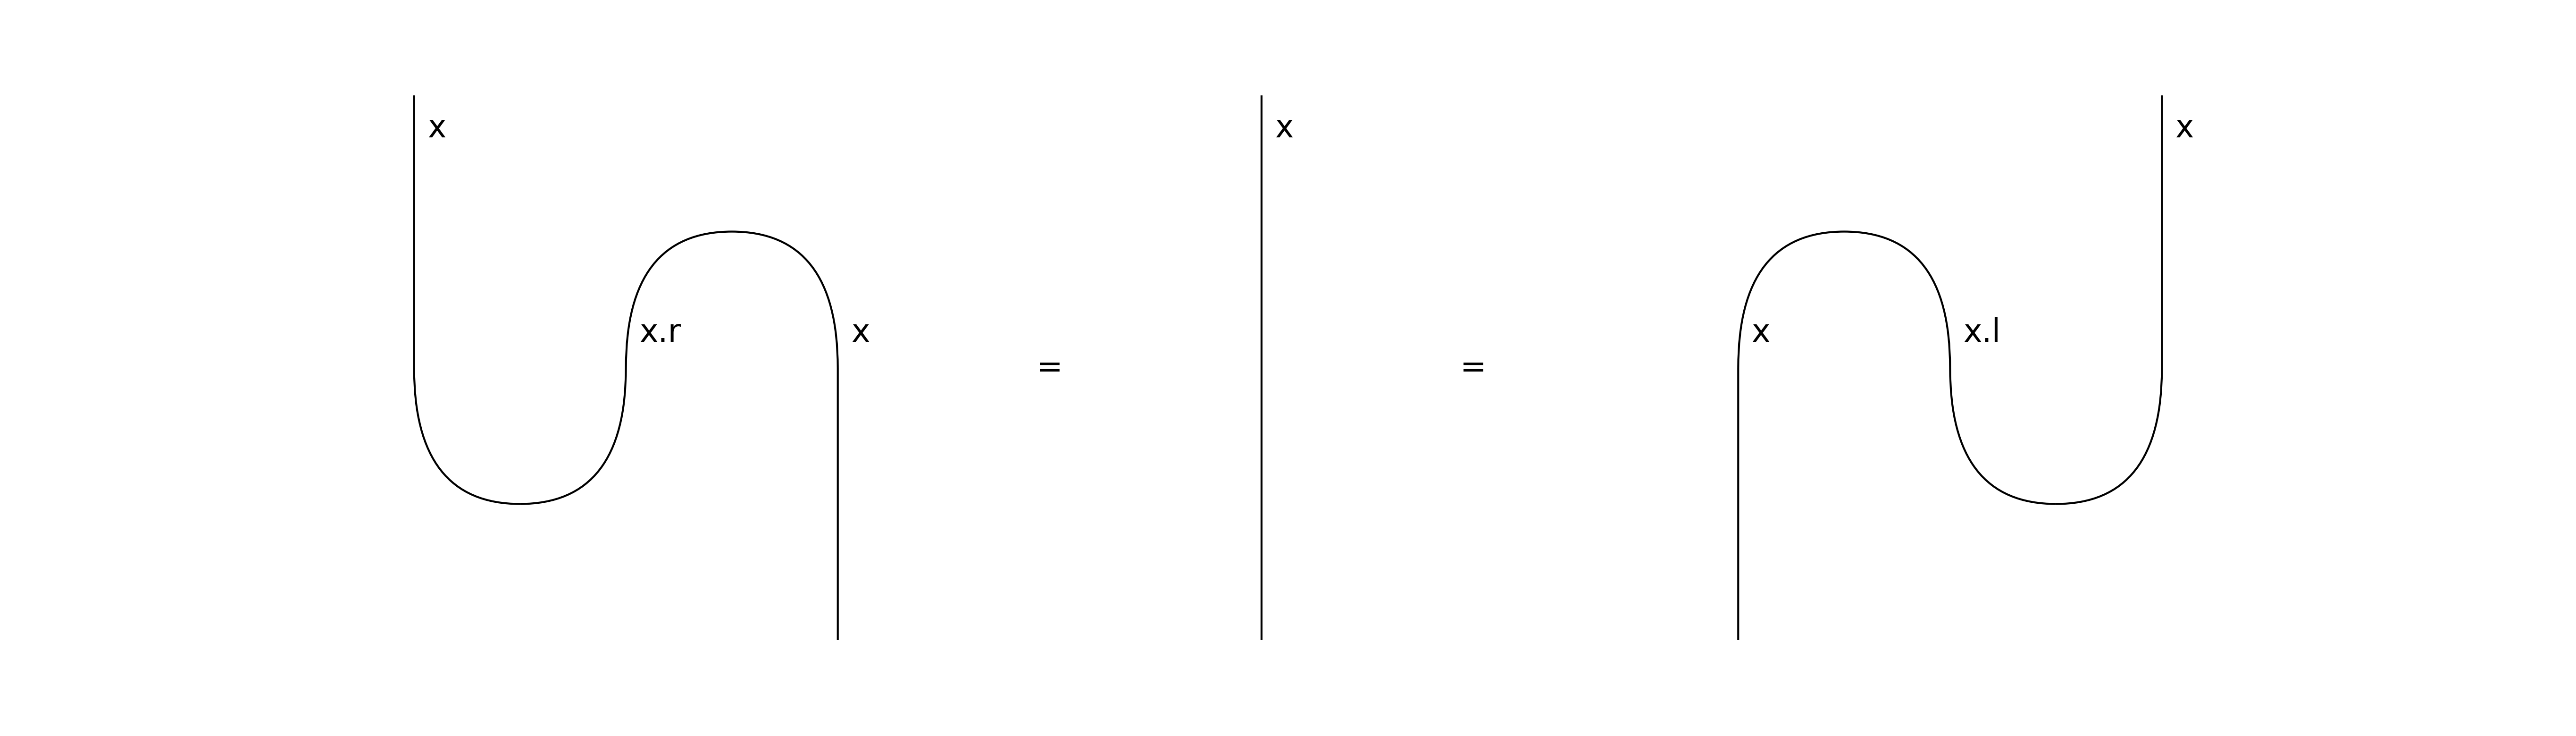
\includegraphics[keepaspectratio,alt={The snake equation is the algebraic engine powering every pregroup type reduction. The compact closure axiom () rendered by DisCoPy as a three-panel equality: left panel shows the right-adjoint zigzag (\textbackslash varepsilon\_n \textbackslash otimes 1\_n) \textbackslash circ (1\_n \textbackslash otimes \textbackslash eta\_n) with the x\^{}r intermediary; middle panel is the identity wire 1\_n that the zigzag equals; right panel shows the mirror-image left-adjoint zigzag using the x\^{}l adjoint. Verified computationally via diagram.normal\_form() == Id(Ty(\textquotesingle x\textquotesingle)). Each pregroup contraction (noun canceling with verb argument) is an instance of \textbackslash varepsilon\{\}; the snake equation guarantees that cup-cap pair insertions and removals leave derivations invariant (cf.~). Generated by render\_discopy\_snake() in src/visualization/discopy\_diagrams.py.}]{../figures/discopy_snake.png}}
\caption{The snake equation is the algebraic engine powering every
pregroup type reduction. The compact closure axiom (\autoref{eq:eq-4-3})
rendered by DisCoPy as a three-panel equality: \textbf{left panel} shows
the right-adjoint zigzag
\((\varepsilon_n \otimes 1_n) \circ (1_n \otimes \eta_n)\) with the
\(x^r\) intermediary; \textbf{middle panel} is the identity wire \(1_n\)
that the zigzag equals; \textbf{right panel} shows the mirror-image
left-adjoint zigzag using the \(x^l\) adjoint. Verified computationally
via
\protect\texttt{diagram.normal\_form()\ ==\ Id(Ty(\textquotesingle{}x\textquotesingle{}))}.
Each pregroup contraction (noun canceling with verb argument) is an
instance of \(\varepsilon{}\); the snake equation guarantees that
cup-cap pair insertions and removals leave derivations invariant
(cf.~\autoref{sec:categorial-grammar}). Generated by
\protect\texttt{render\_discopy\_snake()} in
\protect\texttt{src/visualization/discopy\_diagrams.py}.}\label{fig:discopy-snake}
\end{figure}

\autoref{fig:snake-unpacking} unpacks the same axiom into three explicit
panels: the left-hand zigzag carrying its \(\eta_n\) and
\(\varepsilon_n\) labels, the identity wire \(1_n\) it equals, and an
algebraic recap of both compact-closure equations with cap and cup type
signatures.

\begin{figure}
\centering
\pandocbounded{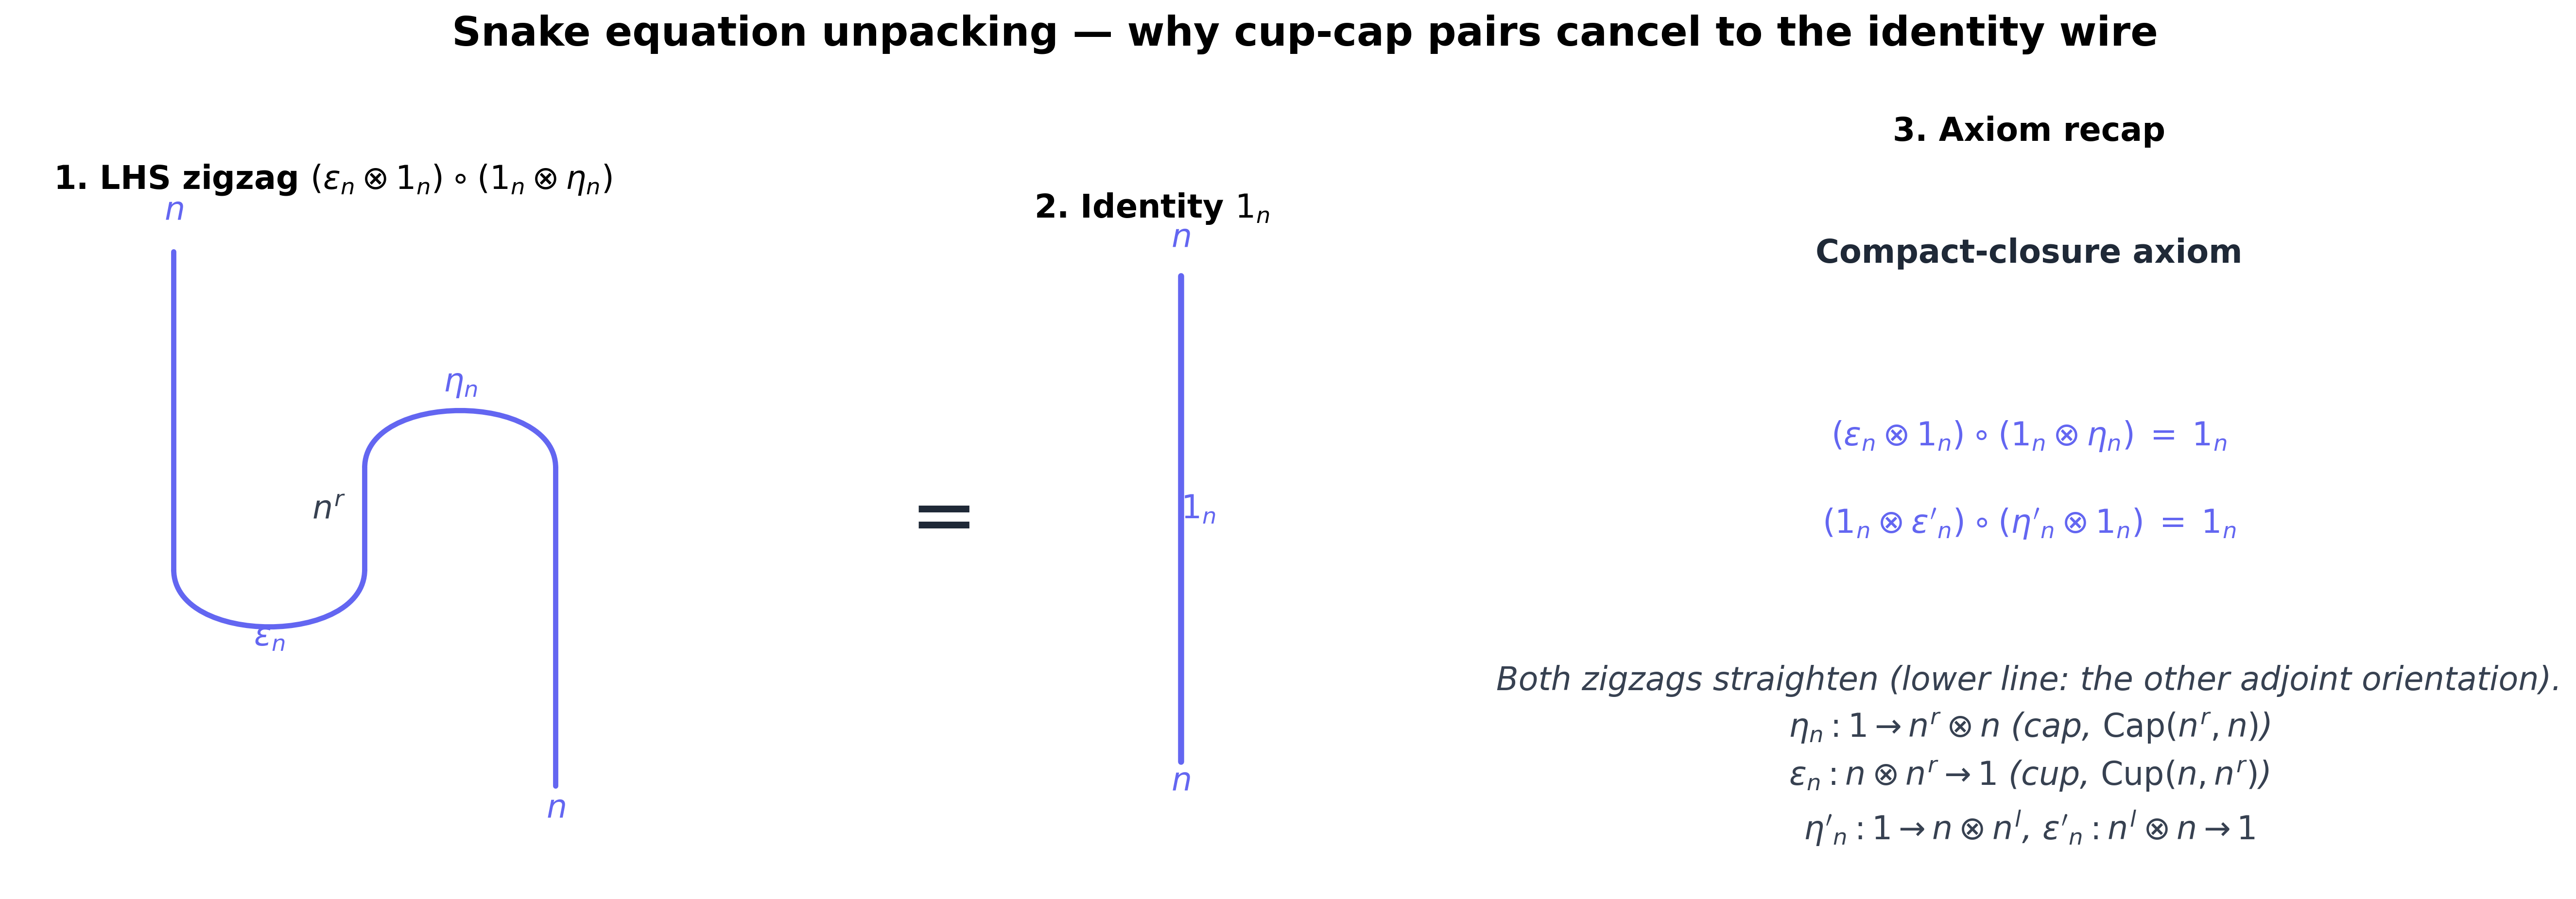
\includegraphics[keepaspectratio,alt={Snake equation unpacked. Panel 1: the zigzag (\textbackslash varepsilon\_n \textbackslash otimes 1\_n) \textbackslash circ (1\_n \textbackslash otimes \textbackslash eta\_n) with \texorpdfstring{\ensuremath{\eta}}{eta} at the top (cap, 1 \textbackslash to n \textbackslash otimes n\^{}r) and \texorpdfstring{\ensuremath{\varepsilon}}{epsilon} at the bottom (cup, n\^{}r \textbackslash otimes n \textbackslash to 1). Panel 2: the identity wire 1\_n it equals. Panel 3: axiom recap showing both zigzag equations straighten to the identity, with explicit type signatures for \texorpdfstring{\ensuremath{\eta}}{eta} and \texorpdfstring{\ensuremath{\varepsilon}}{epsilon}. Generated programmatically from src.visualization.category\_unpacking.render\_snake\_equation\_unpacking().}]{../figures/snake_equation_unpacking.png}}
\caption{Snake equation unpacked. Panel 1: the zigzag
\((\varepsilon_n \otimes 1_n) \circ (1_n \otimes \eta_n)\) with \texorpdfstring{\ensuremath{\eta}}{eta} at the
top (cap, \(1 \to n \otimes n^r\)) and \texorpdfstring{\ensuremath{\varepsilon}}{epsilon} at the bottom (cup,
\(n^r \otimes n \to 1\)). Panel 2: the identity wire \(1_n\) it equals.
Panel 3: axiom recap showing both zigzag equations straighten to the
identity, with explicit type signatures for \texorpdfstring{\ensuremath{\eta}}{eta} and \texorpdfstring{\ensuremath{\varepsilon}}{epsilon}. Generated
programmatically from
\protect\texttt{src.visualization.category\_unpacking.render\_snake\_equation\_unpacking()}.}\label{fig:snake-unpacking}
\end{figure}

\subsubsection{Four Metrics Quantify Derivational
Complexity}\label{four-metrics-quantify-derivational-complexity}

The algebraic properties of pregroup diagrams support quantitative
analysis of derivational complexity. Our \texttt{complexity\_metrics}
module implements four complementary measures using the DisCoPy library:

\begin{enumerate}
\def\labelenumi{\arabic{enumi}.}
\item
  \textbf{Box count}: The number of lexical entries (Word boxes) in the
  diagram, corresponding to the sentence's word count from the
  type-logical perspective. A transitive sentence has 3 boxes (subject,
  verb, object); a ditransitive sentence has 4 or more.
\item
  \textbf{Cup/Cap count}: The number of contraction and expansion
  operations. Cups (denoted \(\varepsilon{}\)) count argument
  consumption; caps (denoted \(\eta{}\)) count argument introduction.
  The cup count directly reflects verb valency: an intransitive verb
  requires 1 cup, a transitive verb 2, and a ditransitive verb 3.
\item
  \textbf{Normal form}: A diagram is in \emph{normal form} if no further
  simplifications (zigzag cancellations, box reordering) are possible.
  The \texttt{compute\_normal\_form()} operation computes this canonical
  representative of the diagram's equivalence class. Normal form
  preservation under algebraic manipulation provides a correctness check
  for compositional operations.
\item
  \textbf{Syntactic complexity score}: A composite metric defined as:
\end{enumerate}

\begin{equation}
\text{complexity}(D) = w_w \cdot |D|_{\text{words}} + w_c \cdot |D|_{\text{cup}} + w_a \cdot |D|_{\text{cap}} + w_d \cdot \text{depth}(D)
\label{eq:eq-4-4}
\end{equation}

where \(|D|_{\text{words}}\) is the \emph{lexical} box count (Cup/Cap
plumbing excluded), \(|D|_{\text{cup}}\) and \(|D|_{\text{cap}}\) are
contraction and expansion counts, and \(\text{depth}(D)\) is the longest
input-to-output path measured in boxes. The weights
\(w_w, w_c, w_a, w_d\) are keyword arguments to
\texttt{syntactic\_complexity\_score()}; the defaults \(w_w{=}1.0\),
\(w_c{=}0.5\), \(w_a{=}0.25\), \(w_d{=}0.1\) encode the intuition that
lexical entries contribute most, contractions moderately, expansions
least, and depth a small residual penalty. Passing
\(w_w{=}w_c{=}w_a{=}w_d{=}1.0\) recovers an unweighted total-structure
count. Deeper diagrams encode more complex syntactic derivations---a
ditransitive sentence like ``Alice gave Bob a book'' (depth 7) is
structurally more complex than a simple intransitive ``Alice runs''
(depth 3).

The \texttt{compare\_diagrams()} function applies these metrics across a
collection of diagrams, producing tabular comparisons suitable for
cross-linguistic analysis. \autoref{fig:complexity-comparison}
visualizes these metrics across sentence types of increasing valency,
demonstrating the monotonic relationship between argument structure and
derivational complexity.

\begin{figure}
\centering
\pandocbounded{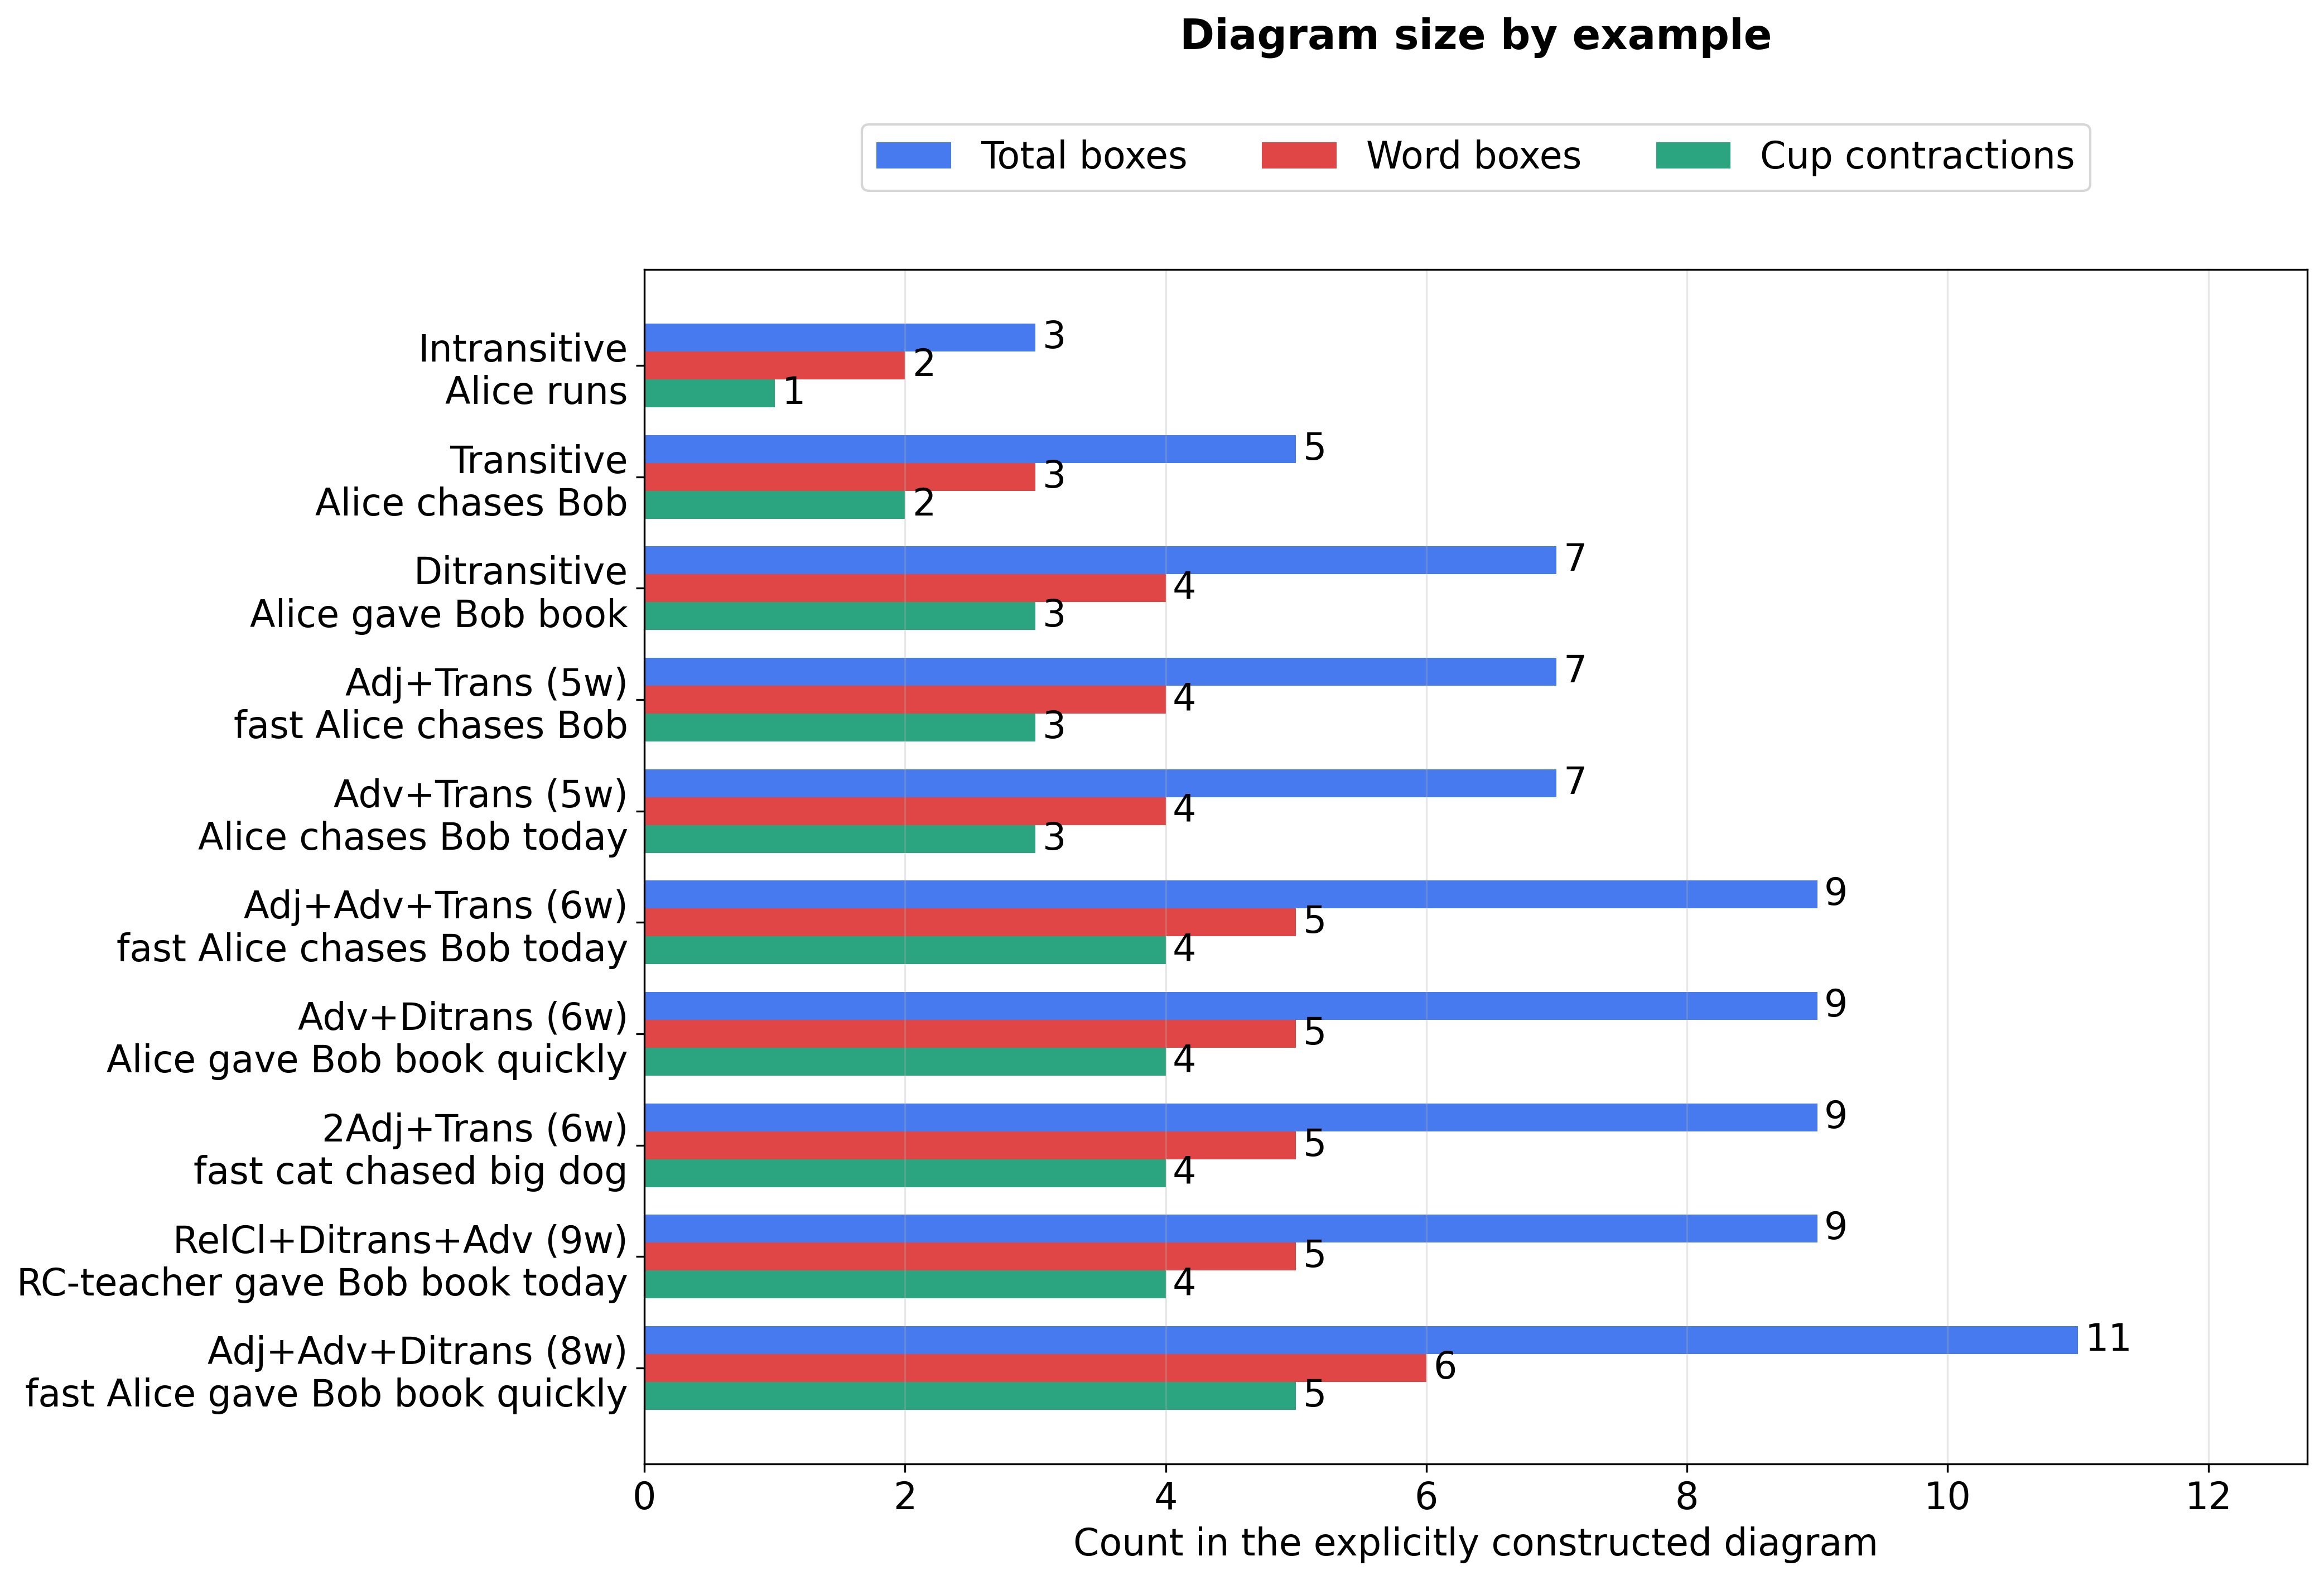
\includegraphics[keepaspectratio,alt={Verb valency dominates diagram complexity: categorical complexity score \textbackslash kappa(D) () plotted for ten sentence types ranging from intransitive to adjunct-heavy constructions, with natural-language exemplar sentences overlaid at each bar. Generated by render\_complexity\_comparison() in src/visualization/complexity\_plots.py (orchestrated by scripts/generate\_diagrams.py).}]{../figures/complexity_comparison.png}}
\caption{Verb valency dominates diagram complexity: categorical
complexity score \(\kappa(D)\) (\autoref{eq:eq-4-4}) plotted for ten
sentence types ranging from intransitive to adjunct-heavy constructions,
with natural-language exemplar sentences overlaid at each bar. Generated
by \protect\texttt{render\_complexity\_comparison()} in
\protect\texttt{src/visualization/complexity\_plots.py} (orchestrated by
\protect\texttt{scripts/generate\_diagrams.py}).}\label{fig:complexity-comparison}
\end{figure}

\textbf{Key finding.} Adverb and adjective modifiers increase box count
but do not always add core argument Cups (modifier types \(n \cdot n^l\)
contribute one box and one cup each, but some adverbs add a box without
an argument Cup), so \(\kappa{}\) can grow more slowly with adjunct
stacking than with valency increases. Cup count
\(\lvert D\rvert_{\text{cup}}\) remains a reliable proxy for verb
valency. In code, cup counts are obtained by iterating DisCoPy diagram
boxes and testing for \texttt{Cup} instances (see
\texttt{compare\_diagrams()} in the project).

These metrics connect naturally to the enriched framework of
\autoref{sec:enriched-categories}: diagram depth serves as a syntactic
complexity proxy that can be incorporated into the enriched hom-value,
providing a principled bridge between type-logical derivation cost and
distributional semantic distance. Discourse-level persistence of entity
wires (DisCoCirc) is developed in \autoref{sec:discocirc-discourse}. For
multi-agent security, when tracking networks isolate an adversarial
identity wire (a prompt injection) covertly attempting to merge with an
ongoing command wire across communication boundaries, the circuit
topology can flag the type violation before execution
(\autoref{sec:cognitive-security}).

\newpage

\section{Beyond the Sentence: State Wires Accumulate Semantic History
Across Discourse}\label{sec:discocirc-discourse}

\textbf{Where we are in the argument.}
\autoref{sec:categorical-semantics}--\autoref{sec:compact-closure-complexity}
formalised individual sentences as compact-closed string diagrams and
their complexity as a four-metric summary. This chapter extends
composition \emph{across} sentence boundaries: de Felice--Coecke
DisCoCirc adds persistent entity wires that carry an entity's case-role
history across a discourse, so that a three-sentence discourse traces
Alice's NOM \texorpdfstring{\ensuremath{\to}}{->} ACC \texorpdfstring{\ensuremath{\to}}{->} NOM trajectory and Bob's ACC \texorpdfstring{\ensuremath{\to}}{->} NOM trajectory as
first-class diagrammatic data rather than coreference annotation bolted
on after the fact.

\subsection{DisCoCirc State Wires Resolve Coreference and Role
Shifts}\label{discocirc-state-wires-resolve-coreference-and-role-shifts}

De Felice and Coecke \citeyearpar{defelice2020discourse} address this
limitation by formulating \textbf{DisCoCirc} (Distributional
Compositional Circuits). DisCoCirc extends the base categorical
framework, empowering it to dynamically handle discourse-level semantic
structure.

Specifically, DisCoCirc introduces continuous \emph{state wires} that
actively persist across isolated sentence boundaries, continuously
encoding the dynamically evolving states of distinct discourse entities
(e.g., characters, objects, shifting topics). For example, a
multi-sentence sequence like ``Alice chased Bob. He was terrified.'' is
explicitly represented as an integrated geometric circuit where:

\begin{itemize}
\tightlist
\item
  Alice and Bob are wires that persist across both sentences.
\item
  The pronoun ``He'' is resolved by actively connecting its topological
  wire directly to Bob's wire.
\item
  The shifting emotional state ``terrified'' seamlessly updates the
  cumulative state information carried exclusively by Bob's persistent
  wire.
\end{itemize}

De Felice et al. \citeyearpar{defelice2022discocirc} subsequently
extended this approach, developing a full-fledged, multi-layered circuit
model built to systematically resolve ambiguity, tangled coreference,
and overarching discourse coherence---all locked within the exact same
continuous categorical formalism. A CCG-based pipeline for generating
discourse circuits from syntactic parse trees has demonstrated that
DisCoCirc can scale to text, dynamically composing sentence-level
diagrams along shared entity wires via an iterative process of
coreference resolution and wire merging \citeyearpar{duneau2021parsing}.
This pipeline approach has since been extended to a comparative
framework for evaluating compositional AI model architectures
\citeyearpar{duneau2025comparative}, confirming that the DisCoCirc
wire-merging strategy generalizes across model families. Complementary
work on \textbf{DiscoSG} (Discourse Scene Graphs) extends this approach
to multi-sentence image captions, parsing text into scene graphs that
capture cross-sentence coreference relations. \autoref{fig:discourse}
illustrates a multi-sentence discourse diagram where entity wires
persist across sentence boundaries. For case theory, DisCoCirc is
significant because it shows how case-marked argument structure
\emph{composes across discourse}: the nominative subject of one sentence
can become the accusative object of the next, and this transformation is
tracked as a morphism in the discourse category.

\begin{figure}
\centering
\pandocbounded{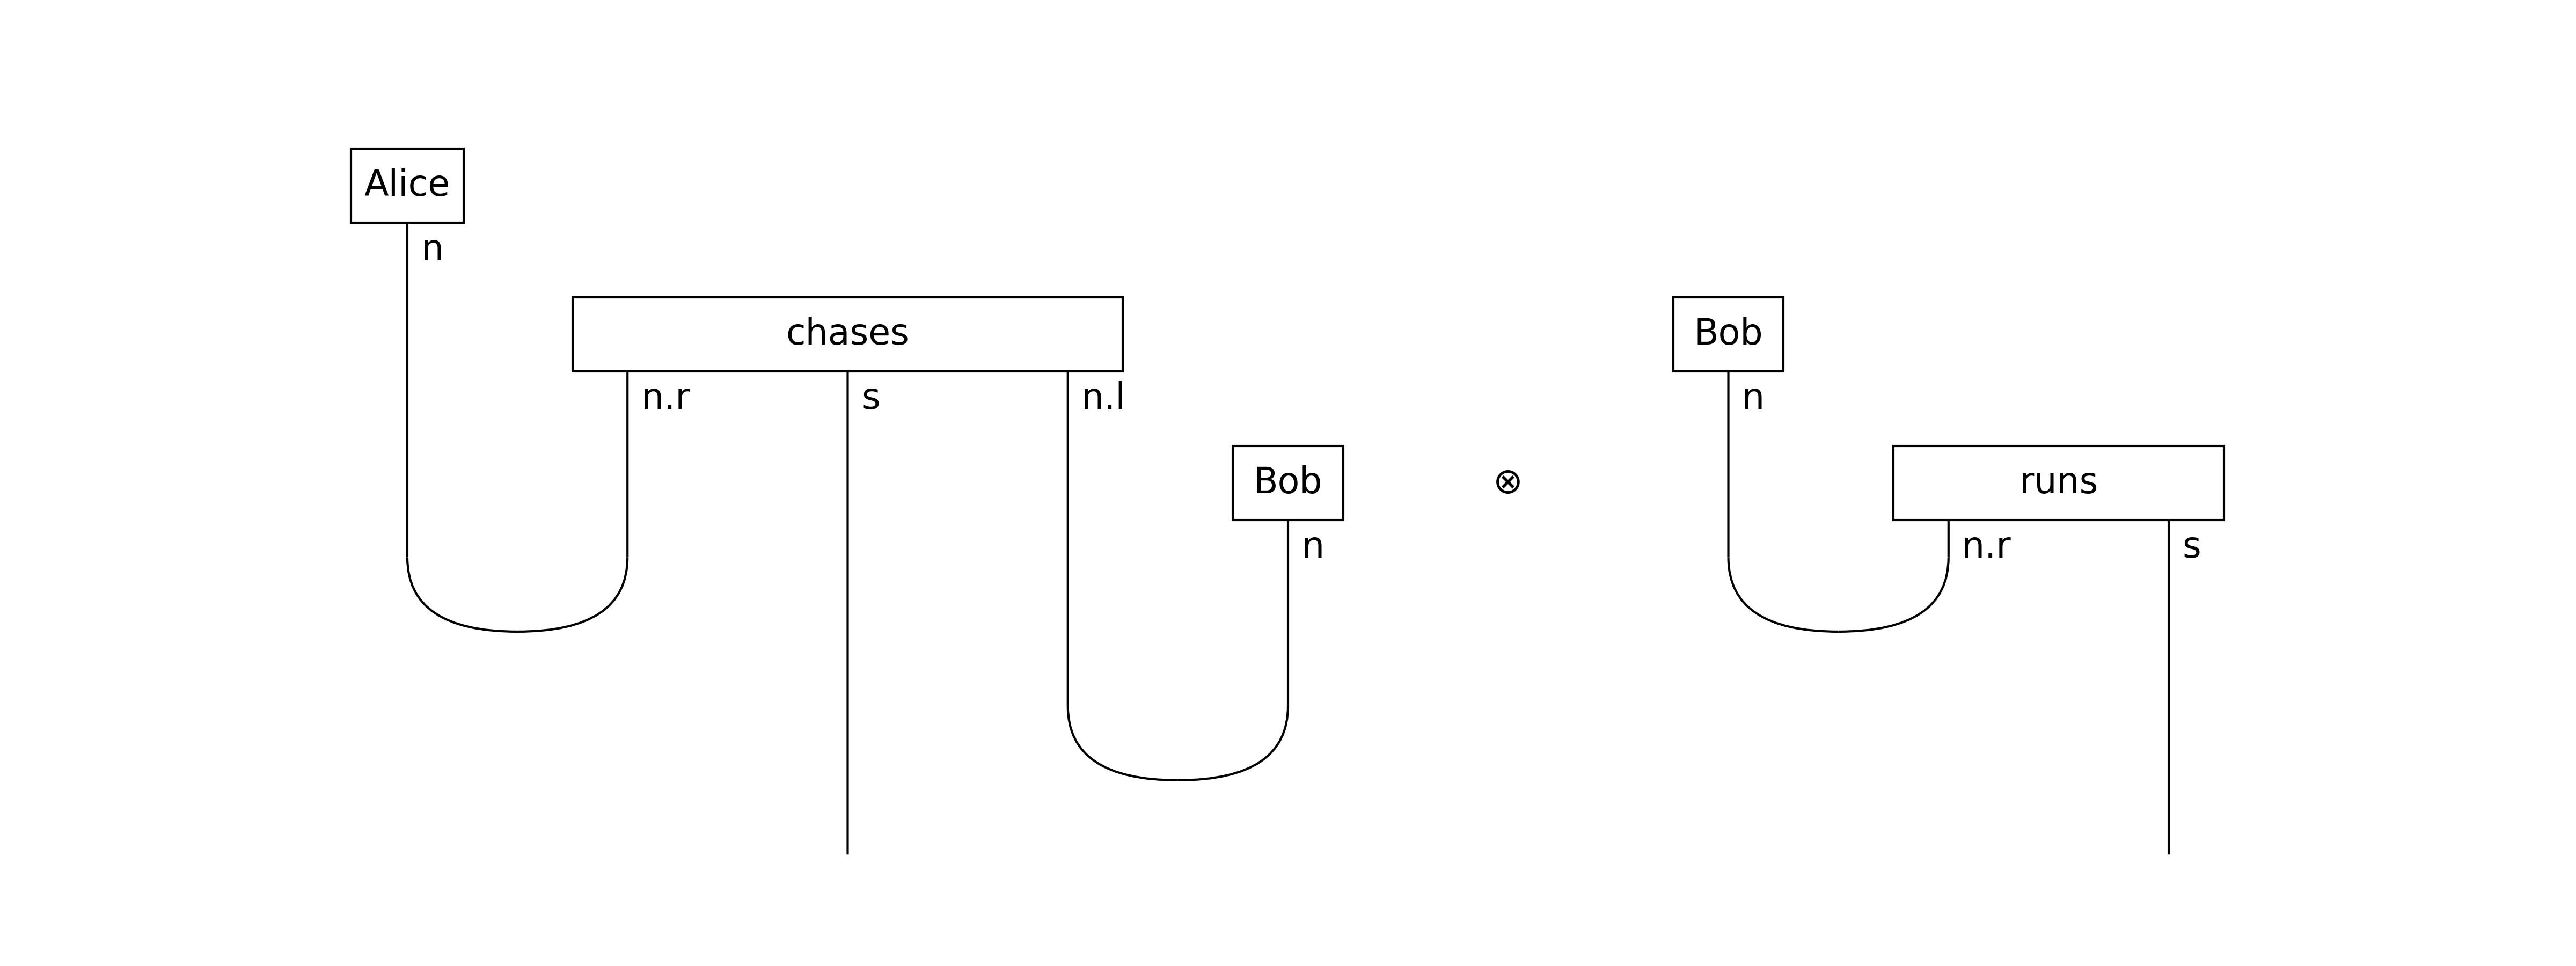
\includegraphics[keepaspectratio,alt={DisCoCirc type structure encodes discourse coherence as a tensor product of sentence types. DisCoPy pregroup grammar for ``Alice chases Bob. Bob runs.'' showing inter-sentential composition. Sentence 1 (left subdiagram): Alice (n) and Bob (n) contract into ``chases'' (n\^{}r \textbackslash otimes s \textbackslash otimes n\^{}l) via two Cups, yielding sentence type s. Sentence 2 (right subdiagram): Bob (n) contracts into ``runs'' (n\^{}r \textbackslash otimes s) via one Cup, yielding s. The joint discourse type s \textbackslash otimes s encodes inter-sentential coherence as a tensor product, the computational primitive that DisCoCirc state wires exploit to propagate Bob's semantic state from ACC (sentence 1) to NOM (sentence 2). See  for wire-colour confirmation of the role transition, and  for the three-sentence DisCoPy tensor layout (role reversal; anaphora is developed in prose and in the Discourse API below, not as a separate pronoun box in the DisCoPy figure).}]{../figures/discopy_discocirc_discourse.png}}
\caption{DisCoCirc type structure encodes discourse coherence as a
tensor product of sentence types. DisCoPy pregroup grammar for ``Alice
chases Bob. Bob runs.'' showing inter-sentential composition.
\textbf{Sentence 1} (left subdiagram): Alice (\(n\)) and Bob (\(n\))
contract into ``chases'' (\(n^r \otimes s \otimes n^l\)) via two Cups,
yielding sentence type \(s\). \textbf{Sentence 2} (right subdiagram):
Bob (\(n\)) contracts into ``runs'' (\(n^r \otimes s\)) via one Cup,
yielding \(s\). The joint discourse type \(s \otimes s\) encodes
inter-sentential coherence as a tensor product, the computational
primitive that DisCoCirc state wires exploit to propagate Bob's semantic
state from ACC (sentence 1) to NOM (sentence 2). See
\autoref{fig:native-discourse} for wire-colour confirmation of the role
transition, and \autoref{fig:three-sentence-discourse} for the
three-sentence DisCoPy tensor layout (role reversal; anaphora is
developed in prose and in the \protect\texttt{Discourse} API below, not
as a separate pronoun box in the DisCoPy figure).}\label{fig:discourse}
\end{figure}

\begin{figure}
\centering
\pandocbounded{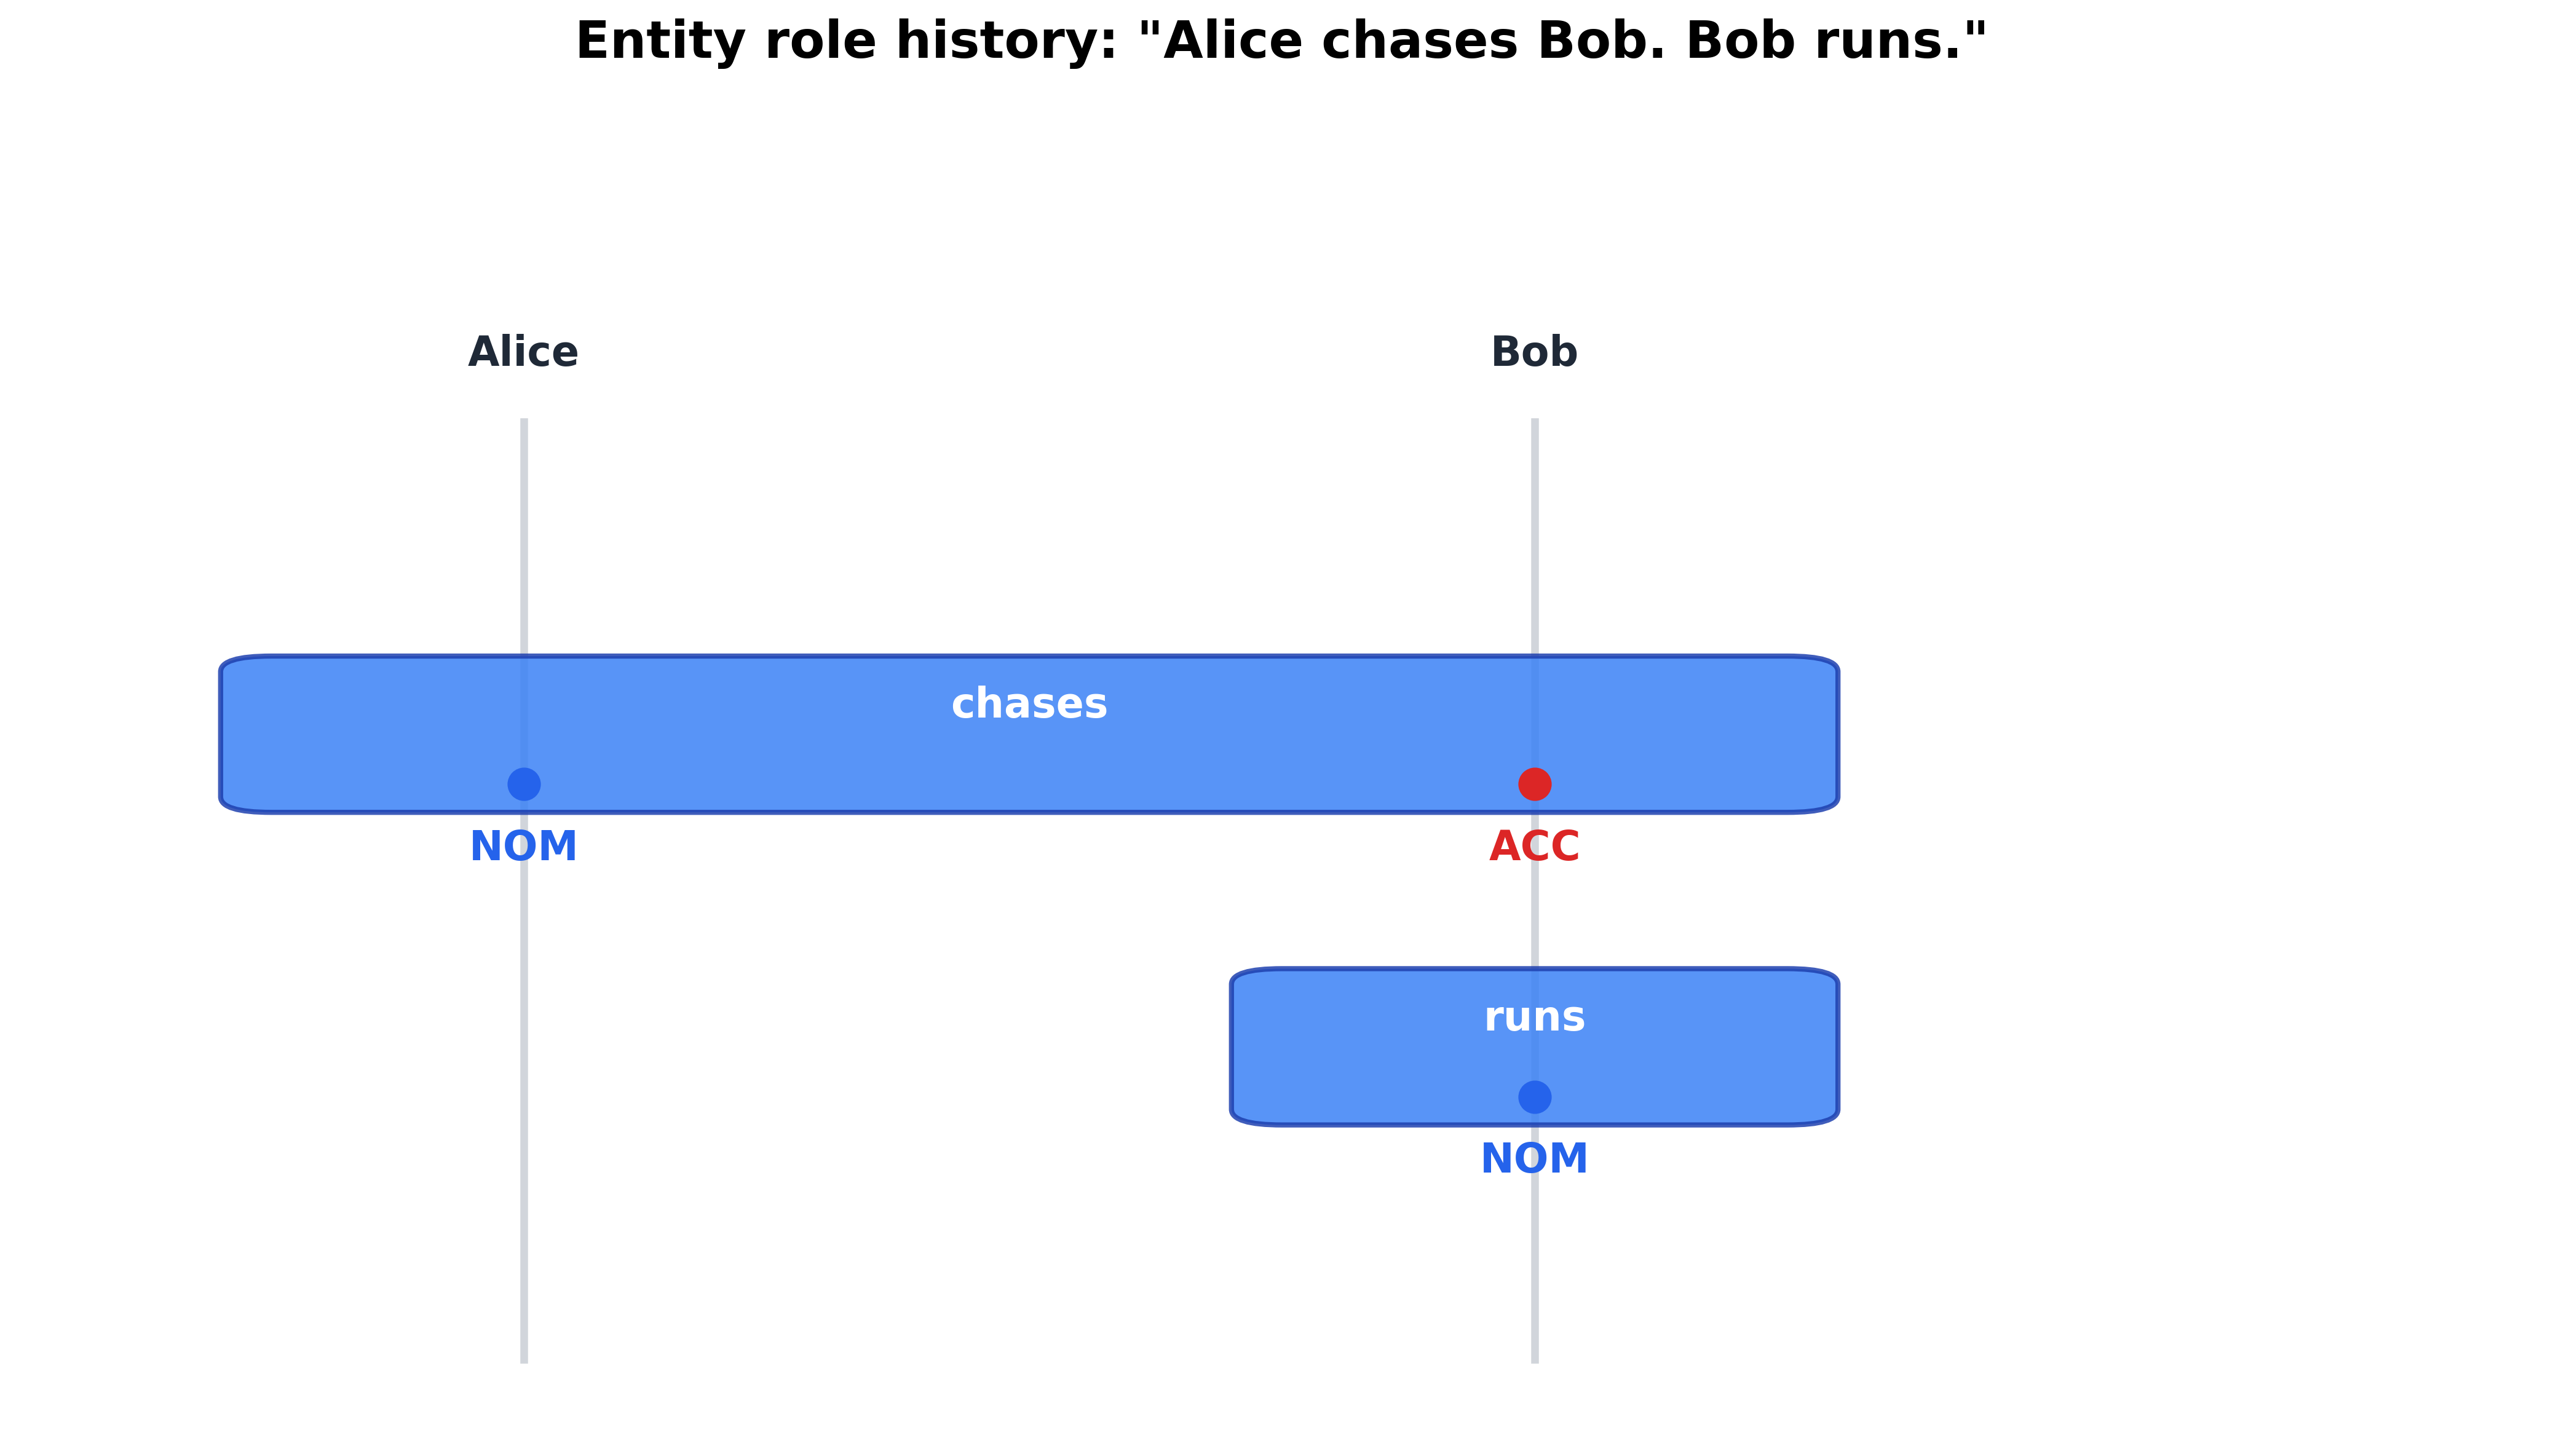
\includegraphics[keepaspectratio,alt={Wire colour provides independent visual confirmation of the ACC\textbackslash toNOM role transition that  encodes algebraically. Native matplotlib DisCoCirc diagram for the same two-sentence discourse, generated via src.visualization.string\_diagrams.render\_discocirc\_discourse() without the DisCoPy library. Vertical grey wires: persistent entity wires for Alice and Bob, confirming that identity is tracked across the sentence boundary. Colour-coded role discs: Bob's wire is marked red (ACC) at sentence 1 (chased object) and blue (NOM) at sentence 2 (running agent). The ACC\textbackslash toNOM colour change is directly readable from the diagram without algebraic computation --- Shimojima's free-ride inference in action. This independent rendering cross-validates that src.diagrams.string\_diagram.Discourse correctly resolves entity identity and role reassignment using only case-role metadata.}]{../figures/discourse_string_diagram.png}}
\caption{Wire colour provides independent visual confirmation of the
ACC\(\to\)NOM role transition that \autoref{fig:discourse} encodes
algebraically. Native matplotlib DisCoCirc diagram for the same
two-sentence discourse, generated via
\protect\texttt{src.visualization.string\_diagrams.render\_discocirc\_discourse()}
without the DisCoPy library. \textbf{Vertical grey wires}: persistent
entity wires for Alice and Bob, confirming that identity is tracked
across the sentence boundary. \textbf{Colour-coded role discs}: Bob's
wire is marked \textbf{red} (ACC) at sentence 1 (chased object) and
\textbf{blue} (NOM) at sentence 2 (running agent). The ACC\(\to\)NOM
colour change is directly readable from the diagram without algebraic
computation --- Shimojima's free-ride inference in action. This
independent rendering cross-validates that
\protect\texttt{src.diagrams.string\_diagram.Discourse} correctly
resolves entity identity and role reassignment using only case-role
metadata.}\label{fig:native-discourse}
\end{figure}

\subsection{Alice's Role Trajectory: NOM\texorpdfstring{\ensuremath{\to}}{->}ACC\texorpdfstring{\ensuremath{\to}}{->}NOM Across Three
Sentences}\label{alices-role-trajectory-nomaccnom-across-three-sentences}

The power of DisCoCirc for case theory becomes particularly vivid in
multi-sentence discourses where the \emph{same entity occupies different
case roles} across sentences. Consider the three-sentence discourse:

\begin{quote}
\emph{``Alice chases Bob. Bob fears Alice. She smiles.''}
\end{quote}

In this discourse, Alice undergoes a complete cycle of case role
reversals:

\begin{enumerate}
\def\labelenumi{\arabic{enumi}.}
\tightlist
\item
  \textbf{Sentence 1}: Alice is \(\text{NOM}\) (Proto-Agent, the one
  chasing) and Bob is \(\text{ACC}\) (Proto-Patient, the one chased).
\item
  \textbf{Sentence 2}: Bob is now \(\text{NOM}\) (the one fearing) and
  Alice is \(\text{ACC}\) (the one feared)---a role reversal where Alice
  moves from agent to patient.
\item
  \textbf{Sentence 3}: ``She'' resolves anaphorically to Alice, who
  returns to \(\text{NOM}\) as the agent of smiling.
\end{enumerate}

This NOM \(\to\) ACC \(\to\) NOM trajectory for Alice across three
sentences is precisely the kind of \emph{dynamic case assignment} that
static single-sentence analyses cannot capture. The categorical
representation as a triple tensor product \(s \otimes s \otimes s\)
(\autoref{fig:three-sentence-discourse}) encodes each sentence as an
independent pregroup derivation while preserving the entity identity
that links them. This role reversal essentially requires applying the
topological \texttt{Swap} operation (introduced for passivization in
\autoref{sec:case-type-logic}) dynamically across the discourse
boundary. In a full DisCoCirc implementation, Alice's entity wire would
carry accumulated semantic state---the meaning of ``She'' in sentence 3
inherits the enriched state of an Alice who has first chased and then
been feared, not merely the bare lexical entry for ``Alice.''

The trajectory is \emph{executable}: the
\texttt{src.diagrams.string\_diagram.Discourse} class implements exactly
this entity-wire-with-role-history bookkeeping. The following snippet,
taken verbatim from the public API exercised by the test suite, builds
the three-sentence Alice/Bob discourse and reads back the role history
that drives \autoref{fig:three-sentence-discourse}:

\begin{Shaded}
\begin{Highlighting}[]
\ImportTok{from}\NormalTok{ src.diagrams.string\_diagram }\ImportTok{import}\NormalTok{ Sentence, Discourse}

\NormalTok{discourse }\OperatorTok{=}\NormalTok{ Discourse()}
\NormalTok{discourse.add\_sentence(Sentence.transitive(}\StringTok{"Alice"}\NormalTok{, }\StringTok{"chases"}\NormalTok{, }\StringTok{"Bob"}\NormalTok{))}
\NormalTok{discourse.add\_sentence(Sentence.transitive(}\StringTok{"Bob"}\NormalTok{, }\StringTok{"fears"}\NormalTok{, }\StringTok{"Alice"}\NormalTok{))}
\NormalTok{discourse.add\_sentence(Sentence.intransitive(}\StringTok{"Alice"}\NormalTok{, }\StringTok{"smiles"}\NormalTok{))}

\CommentTok{\# Persistent entity wires (DisCoCirc state{-}wire reading)}
\ControlFlowTok{assert}\NormalTok{ discourse.entities }\OperatorTok{==}\NormalTok{ \{}\StringTok{"Alice"}\NormalTok{, }\StringTok{"Bob"}\NormalTok{\}}
\ControlFlowTok{assert}\NormalTok{ discourse.num\_sentences }\OperatorTok{==} \DecValTok{3}

\CommentTok{\# Role history per entity reproduces the NOM → ACC → NOM trajectory}
\ControlFlowTok{assert}\NormalTok{ [r.name }\ControlFlowTok{for}\NormalTok{ r }\KeywordTok{in}\NormalTok{ discourse.role\_history[}\StringTok{"Alice"}\NormalTok{]] }\OperatorTok{==}\NormalTok{ [}\StringTok{"NOM"}\NormalTok{, }\StringTok{"ACC"}\NormalTok{, }\StringTok{"NOM"}\NormalTok{]}
\ControlFlowTok{assert}\NormalTok{ [r.name }\ControlFlowTok{for}\NormalTok{ r }\KeywordTok{in}\NormalTok{ discourse.role\_history[}\StringTok{"Bob"}\NormalTok{]]   }\OperatorTok{==}\NormalTok{ [}\StringTok{"ACC"}\NormalTok{, }\StringTok{"NOM"}\NormalTok{]}

\CommentTok{\# \textasciigrave{}role\_reversal\_entities\textasciigrave{} flags every entity whose case role}
\CommentTok{\# changes across the discourse — the formal analogue of the}
\CommentTok{\# trajectory pictured in \textbackslash{}autoref\{fig:three{-}sentence{-}discourse\}.}
\ControlFlowTok{assert} \BuiltInTok{set}\NormalTok{(discourse.role\_reversal\_entities()) }\OperatorTok{==}\NormalTok{ \{}\StringTok{"Alice"}\NormalTok{, }\StringTok{"Bob"}\NormalTok{\}}
\end{Highlighting}
\end{Shaded}

Slavic discourse supplies a \emph{morphologically overt} analogue of the
persistent state wire: in Serbian/BCS, second-position clitics
(Wackernagel position) such as \emph{je} AUX.3SG, \emph{mu} DAT.3SG.M,
\emph{ga} ACC.3SG.M form a fixed-order cluster that \emph{carries the
case role of the discourse referent forward in time}. \emph{Marko ga je
video} ``Marko him.ACC AUX saw'' and \emph{Dao mu ga je} ``He gave
him.DAT it.ACC AUX'' make Bob's wire-and-case-history visible in the
surface string in a way that English pronouns (which collapse case
morphology onto a tiny three-form \texttt{I/me/my} paradigm) cannot.
Russian, which lacks the BCS clitic cluster, instead encodes the same
persistence directly in the suffix on the noun or full pronoun
(\emph{ego} ACC, \emph{emu} DAT, \emph{im} INS), so role reversals like
Alice's NOM\(\to\)ACC\(\to\)NOM trajectory in \emph{Alisa gonyaet Boba.
Bob boitsja Alisy. Ona ulybaetsja} are reconstructible \emph{from the
morphology alone}, with no positional ambiguity. These are the cleanest
natural-language witnesses for the entity-wire-with-role-history
bookkeeping that the \texttt{Discourse} API formalises.

The point of including the snippet in prose is reproducibility, not
novelty: every assertion above is exercised in
\texttt{tests/test\_diagrams\_string\_diagram.py}, so a reader who
clones the repository can re-derive the discourse-level role
trajectories with no additional setup beyond \texttt{uv\ sync}. The same
\texttt{Discourse} object is what
\texttt{src.visualization.string\_diagrams.render\_discocirc\_discourse()}
consumes to produce \autoref{fig:native-discourse} --- closing the loop
between symbolic case assignment, computational state-wire bookkeeping,
and the colour-coded role transitions visible in the diagram.

\begin{figure}
\centering
\pandocbounded{\includegraphics[keepaspectratio,alt={Dynamic case role reversal tracks entity identity across three-sentence discourse. DisCoPy rendering with lexical heads matching the discourse above: ``Alice chases Bob. Bob fears Alice. Alice smiles.'' (sentence 3 uses the subject node ---same referent as anaphoric  in the running text; DisCoPy boxes are lexical, not pronominal). Sentence 1: Alice NOM, Bob ACC. Sentence 2: Bob NOM, Alice ACC---a complete agent--patient reversal. Sentence 3: Alice NOM as agent of . Alice's trajectory NOM\textbackslash toACC\textbackslash toNOM is tracked by the triple tensor s \textbackslash otimes s \textbackslash otimes s. In a full DisCoCirc implementation, Alice's entity wire carries accumulated semantic state---``She'' in the gloss inherits the enriched state of an Alice who has both chased and been feared. This dynamic case assignment across discourse boundaries is what lambeq Gen II \[@lambeq2025genii\] compiles into parameterized quantum circuits.}]{../figures/discopy_three_sentence_discourse.png}}
\caption{Dynamic case role reversal tracks entity identity across
three-sentence discourse. DisCoPy rendering with lexical heads matching
the discourse above: ``Alice chases Bob. Bob fears Alice. Alice
smiles.'' (sentence 3 uses the subject node \emph{Alice}---same referent
as anaphoric \emph{She} in the running text; DisCoPy boxes are lexical,
not pronominal). \textbf{Sentence 1}: Alice NOM, Bob ACC.
\textbf{Sentence 2}: Bob NOM, Alice ACC---a complete agent--patient
reversal. \textbf{Sentence 3}: Alice NOM as agent of \emph{smiles}.
Alice's trajectory NOM\(\to\)ACC\(\to\)NOM is tracked by the triple
tensor \(s \otimes s \otimes s\). In a full DisCoCirc implementation,
Alice's entity wire carries accumulated semantic state---``She'' in the
gloss inherits the enriched state of an Alice who has both chased and
been feared. This dynamic case assignment across discourse boundaries is
what lambeq Gen II \citep{lambeq2025genii} compiles into parameterized
quantum circuits.}\label{fig:three-sentence-discourse}
\end{figure}

The DisCoPy rendering encodes entity persistence \emph{algebraically}
(each sentence contributes a tensor factor \(s_i\) and the entity wires
are shared by construction), but the reader must infer the shared-entity
structure from context. \autoref{fig:discocirc-persistence} makes the
structure \emph{visual}: each entity is given its own colour (Alice
indigo, Bob amber), the three sentence panels sit side-by-side with cups
coloured by the entity each one contracts, and the bottom
\emph{role-history ribbon} explicitly plots Alice's NOM \(\to\) ACC
\(\to\) NOM trajectory and Bob's ACC \(\to\) NOM trajectory with the
case-role palette used throughout the paper. It is the same object as
\autoref{fig:three-sentence-discourse} --- re-presented with the
Frobenius-spider entity-identity bookkeeping that DisCoCirc posits, made
graphically explicit.

\begin{figure}
\centering
\pandocbounded{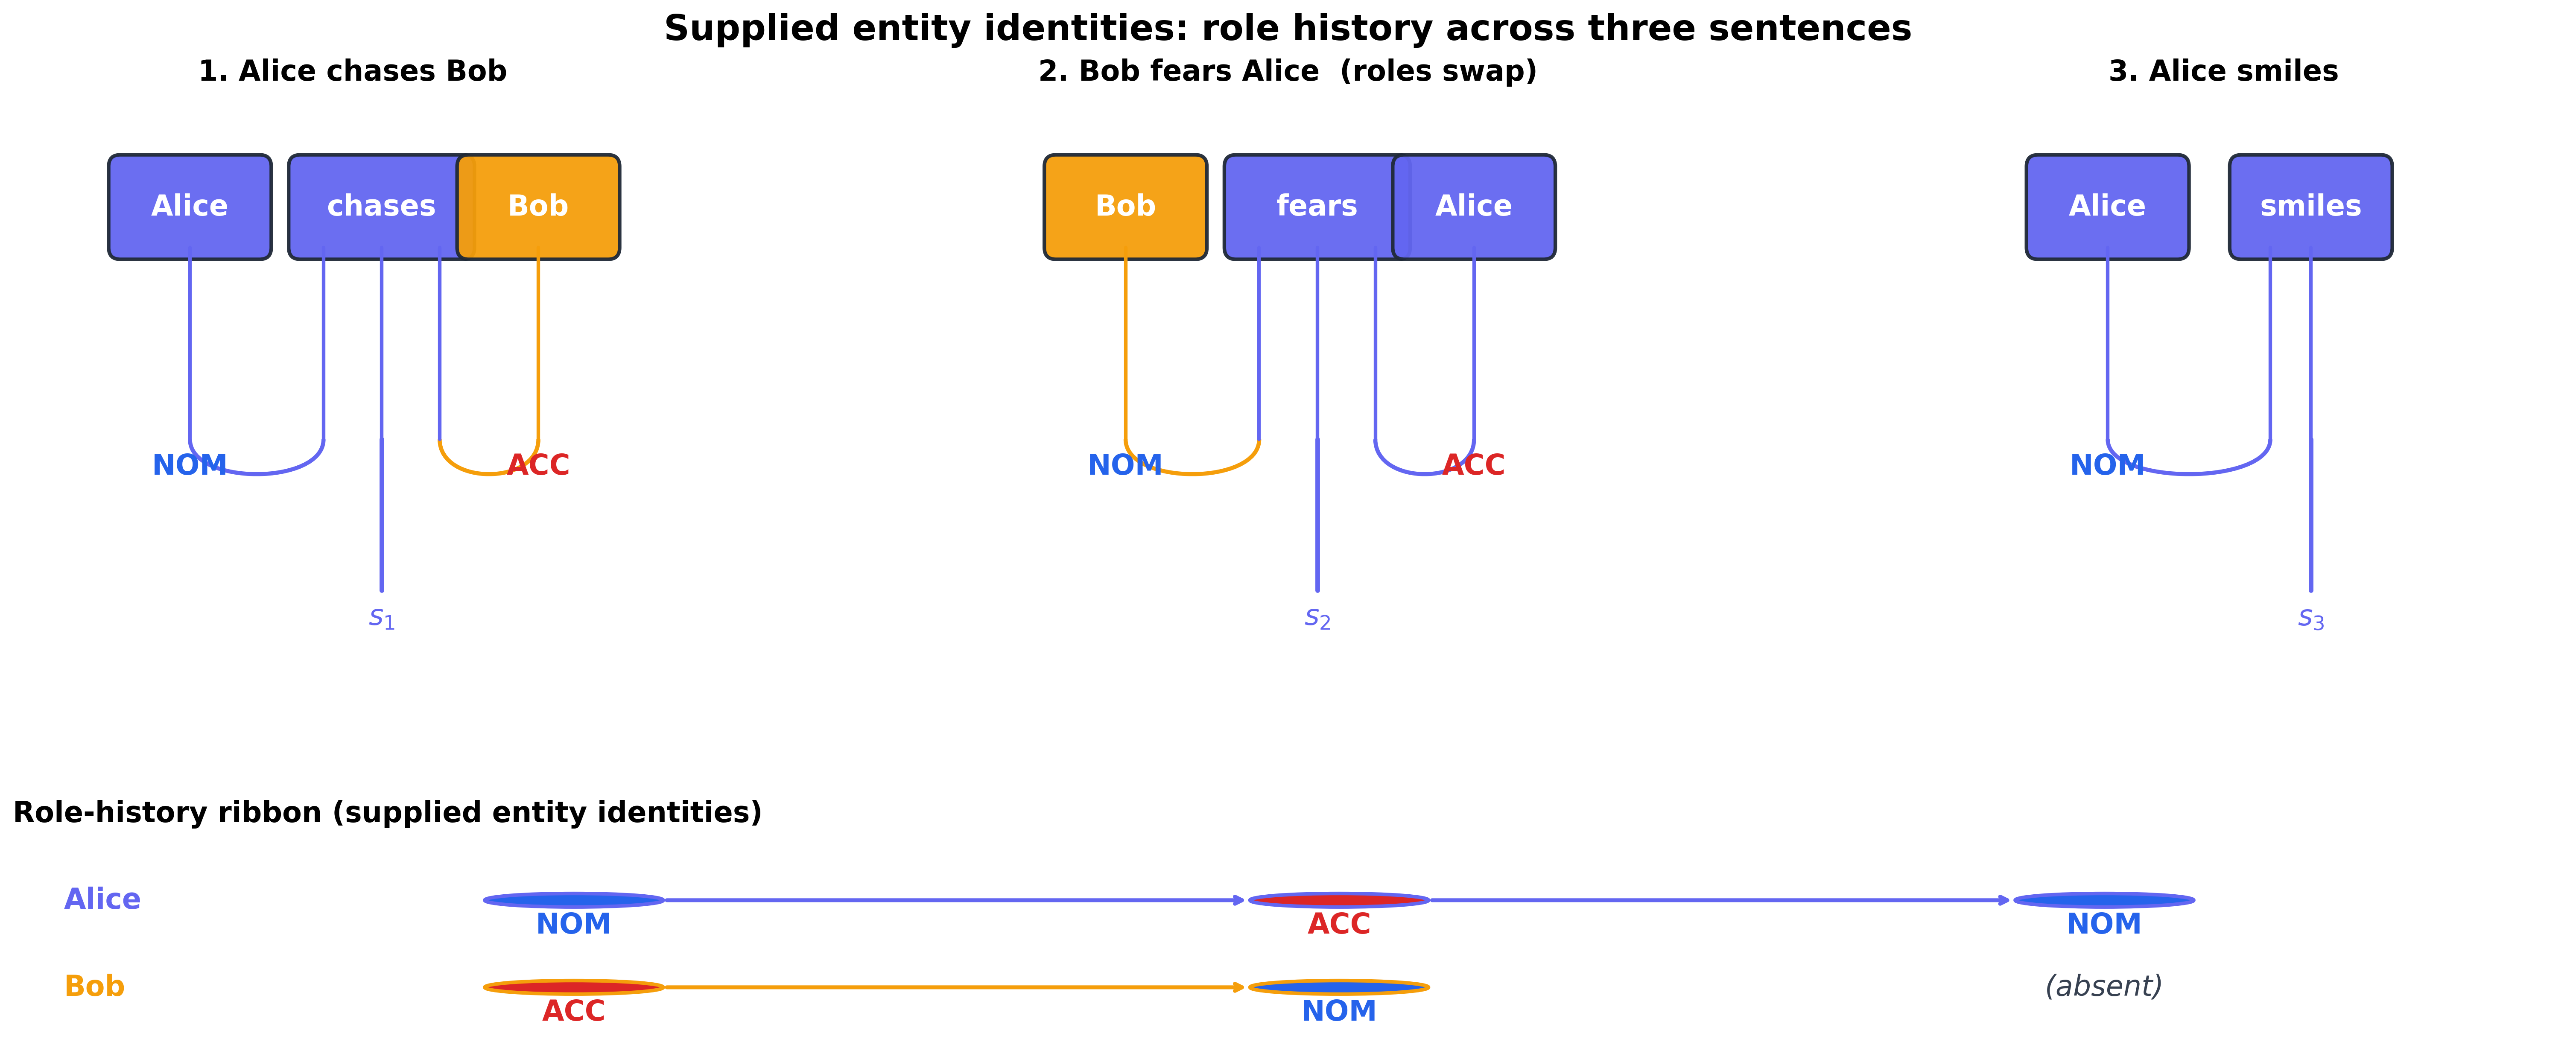
\includegraphics[keepaspectratio,alt={DisCoCirc entity-persistence unpacking for Alice chases Bob. Bob fears Alice. Alice smiles. Three sentence panels (top) plus a role-history ribbon (bottom). Each entity has a dedicated colour (Alice indigo, Bob amber) and the cup contractions are coloured by the entity each one consumes. The ribbon shows Alice traversing NOM\texorpdfstring{\ensuremath{\to}}{->}ACC\texorpdfstring{\ensuremath{\to}}{->}NOM and Bob traversing ACC\texorpdfstring{\ensuremath{\to}}{->}NOM (with an ``absent'' marker for sentence 3), exhibiting graphically the Frobenius-spider entity persistence that motivates DisCoCirc. Generated programmatically from src.visualization.category\_unpacking.render\_discocirc\_entity\_persistence().}]{../figures/discocirc_entity_persistence.png}}
\caption{DisCoCirc entity-persistence unpacking for \emph{Alice chases
Bob. Bob fears Alice. Alice smiles.} Three sentence panels (top) plus a
role-history ribbon (bottom). Each entity has a dedicated colour (Alice
indigo, Bob amber) and the cup contractions are coloured by the entity
each one consumes. The ribbon shows Alice traversing NOM\texorpdfstring{\ensuremath{\to}}{->}ACC\texorpdfstring{\ensuremath{\to}}{->}NOM and Bob
traversing ACC\texorpdfstring{\ensuremath{\to}}{->}NOM (with an ``absent'' marker for sentence 3),
exhibiting graphically the Frobenius-spider entity persistence that
motivates DisCoCirc. Generated programmatically from
\protect\texttt{src.visualization.category\_unpacking.render\_discocirc\_entity\_persistence()}.}\label{fig:discocirc-persistence}
\end{figure}

\subsection{lambeq Gen II Compiles DisCoCirc Discourse
Diagrams}\label{lambeq-gen-ii-compiles-discocirc-discourse-diagrams}

The categorical structure of DisCoCat maps naturally onto quantum
circuits: the tensor product structure of \(\mathbf{FVect}\) is
identical to the tensor product structure of \(\mathbf{Qubit}\), the
category of qubit systems. This observation underlies the \textbf{QNLP}
(Quantum Natural Language Processing) program
\citep{meichanetzidis2020qnlp}, which implements DisCoCat models as
parameterized quantum circuits.

The \textbf{lambeq} library \citep{lorenz2021lambeq} provides a
practical pipeline:

\begin{enumerate}
\def\labelenumi{\arabic{enumi}.}
\tightlist
\item
  Parse a sentence into a pregroup derivation (via the neural CCG parser
  Bobcat or rule-based parsers)
\item
  Convert the derivation into a string diagram
\item
  Translate the diagram into a parameterized quantum circuit (or a
  classical tensor network)
\item
  Train the parameters on NLP tasks (classification, similarity,
  question answering)
\end{enumerate}

Kartsaklis et al. \citeyearpar{kartsaklis2021functorial} demonstrate
that this pipeline achieves competitive performance on
question-answering tasks, confirming that the categorical structure
captures genuine linguistic regularities even when instantiated on noisy
near-term quantum hardware.

\textbf{lambeq Gen II} (released May 21, 2025 by Quantinuum) marks a
significant advance by incorporating full \textbf{DisCoCirc} support as
its core mathematical foundation, enabling the framework to scale beyond
single-sentence semantics to discourse-level NLP
\citep{lambeq2025genii, quantinuum2025genii}. With over 50,000
downloads, lambeq Gen II achieves language neutrality, improved
trainability, and compositional interpretability for explainable AI on
quantum hardware. The new \texttt{DisCoCircReader} API automatically
compiles long texts and multi-page documents into discourse-level
quantum circuits, with entity wires tracking semantic state persistence
across sentence boundaries---closing the gap between sentence-level
DisCoCat and discourse-level case role tracking. This is directly
relevant to the case role reversal phenomena discussed in
\autoref{fig:three-sentence-discourse}: lambeq Gen II can, in principle,
compile such multi-sentence case-dynamic discourses into trainable
quantum circuits.

Foundational work by Meyer and Lewis integrates DisCoCat with density
matrices for modeling dynamic meaning and lexical ambiguity in text,
treating semantic states as mixed quantum states---providing an
alternative to pure-state vector models that naturally accommodates
ambiguity and partial information \citeyearpar{meyer2020modelling}.

Recent work on \textbf{string diagram rewriting} by Bonchi et al.
\citeyearpar{bonchi2022rewriting} provides the theoretical foundation
for diagram simplification, showing that string diagram rewrite systems
modulo Frobenius structure can be interpreted as double-pushout
hypergraph rewriting---ensuring that the algebraic simplifications
applied during normal form computation are provably sound. De Huybrecht
\citeyearpar{dehuybrecht2024subcategorizing} extends DisCoCat with
\emph{subcategorization} for light verb constructions, demonstrating
that the categorical framework accommodates sublexical compositional
structure---a development that connects naturally to the monadic root
syntax of Song \citeyearpar{song2022act} discussed in
\autoref{sec:categorial-grammar}.

For our case-theoretic framework, QNLP offers a concrete computational
substrate: case categories could be implemented as quantum circuits
where case roles correspond to quantum registers and grammatical
relations correspond to parameterized gates. This connection between
linguistic case structure and quantum information processing---mediated
entirely by the shared categorical formalism---illustrates the power of
the diagrammatic approach.

\subsection{No Barren Plateau for Local
Observables}\label{no-barren-plateau-for-local-observables}

A central challenge for practical QNLP on near-term quantum hardware is
the \emph{trainability} of parameterized quantum circuits (PQCs): the
vanishing gradient problem, or \emph{barren plateau}, makes
gradient-based optimization exponentially hard as circuit width and
depth scale. Two recent results (2024) directly resolve this obstacle
for linguistically motivated circuits:

\begin{enumerate}
\def\labelenumi{\arabic{enumi}.}
\item
  \textbf{Rad et al. \citeyearpar{rad2024trainability}} introduce
  \emph{reduced-domain parameter initialization}: rather than sampling
  all parameters uniformly from \([0, 2\pi)\), one initializes the
  circuit in a small-angle domain close to the identity. For circuits of
  the depth typical of DisCoCirc discourse diagrams (compiled from
  multi-sentence texts via coreference resolution), this initialization
  provably yields polynomial rather than exponential gradient
  decay---keeping optimization tractable as discourse length grows.
\item
  \textbf{Letcher et al. \citeyearpar{letcher2024tight}} derive tight,
  \emph{assumption-free} lower bounds on the variance of cost function
  gradients for PQCs with local observables (e.g., Pauli operators
  restricted to a few-qubit subsystem). Their key finding is that, for
  POVMs restricted to local observables---exactly the structure of the
  case-role measurement operators \(E_c\) of \autoref{eq:eq-8-1}
  (formalized in \autoref{sec:quantum-semantics})---no barren plateau
  effect occurs. This provides a theoretical guarantee that case-role
  classification circuits implemented via lambeq remain optimizable
  regardless of total circuit size, so long as the readout observable is
  local.
\end{enumerate}

Together, these results underpin the practical feasibility of the F1 and
F3 research directions of \autoref{sec:conclusion}: scaling case-marked
DisCoCat/DisCoCirc models to corpora-scale quantum hardware without
exponential gradient overhead. The geometric structure of lambeq's IQP
and Sim4 ansätze, combined with these initialization and observable
choices, provides a principled recipe for quantum case category training
on near-term devices.

\newpage

\newpage

\section{\texorpdfstring{\([0,1]\)-Enriched Case Categories: Hom-Values
as Distributional
Proximity}{{[}0,1{]}-Enriched Case Categories: Hom-Values as Distributional Proximity}}\label{sec:enriched-categories}

\textbf{Where we are in the argument.}
\autoref{sec:case-systems}--\autoref{sec:discocirc-discourse} have been
working in a category whose morphisms are Boolean --- a relation either
exists between two case roles or it does not. This chapter upgrades that
to \([0,1]\)-enrichment so every pair of roles carries a \emph{graded}
hom-value \(\mathcal{C}(A, B) \in [0,1]\) --- a distributional proximity
that doubles as the precision \(w_f\) used throughout
\autoref{sec:cognitive-integration} / \autoref{sec:daif-results} for
prediction-error weighting, and that will feed into the magnitude
invariant of \autoref{sec:magnitude-homology} and the topos-theoretic
bridge of \autoref{sec:topos-theory}.

\subsection{Why Binary Morphisms Are Not
Enough}\label{why-binary-morphisms-are-not-enough}

The categories established in \autoref{sec:case-systems}---modeling case
roles as objects and grammatical relations as morphisms---capture the
\emph{qualitative} topology of case systems: which roles exist and how
they connect. However, actual linguistic data is fundamentally
\emph{quantitative}: certain grammatical relations are more probable
than others, proto-role assignments vary in strength, and distributional
similarity is a matter of degree.

To accommodate this quantitative dimension without sacrificing algebraic
structure, we advance from ordinary categories to \textbf{enriched
categories}. In an enriched category, hom-sets carry additional
measurable structure rather than functioning as mere discrete sets of
morphisms. The framework of Bradley et al.
\citeyearpar{fritz2021enriched} supplies the key formal construction.

\subsection{\texorpdfstring{Enriching Over \(([0,1],\cdot,1)\):
Identity, Sub-Multiplicative Composition, and Four Hom-Value
Readings}{Enriching Over ({[}0,1{]},\textbackslash cdot,1): Identity, Sub-Multiplicative Composition, and Four Hom-Value Readings}}\label{enriching-over-01cdot1-identity-sub-multiplicative-composition-and-four-hom-value-readings}

\subsubsection{\texorpdfstring{The Identity and Composition Axioms for
\([0,1]\)-Enriched Case
Categories}{The Identity and Composition Axioms for {[}0,1{]}-Enriched Case Categories}}\label{the-identity-and-composition-axioms-for-01-enriched-case-categories}

A category \(\mathcal{C}\) enriched over the unit interval
\(([0,1], \cdot, 1)\) assigns to every pair of objects \(A, B\) a
\emph{hom-value} \(\mathcal{C}(A, B) \in [0,1]\) satisfying:

\begin{align}
\mathcal{C}(A, A) &= 1 \quad \text{(Identity)} \label{eq:eq-5-1} \\
\mathcal{C}(A, C) &\geq \mathcal{C}(A, B) \cdot \mathcal{C}(B, C) \quad \text{(Composition)} \label{eq:eq-5-2}
\end{align}

The identity axiom dictates that every linguistic expression remains
maximally related to itself. The composition inequality imposes a strict
logical boundary, demanding that distributional relatedness inherently
composes sub-multiplicatively: if expression \(A\) proves 80\% related
to \(B\), and \(B\) remains 70\% related to \(C\), the overarching
algebraic structure formally guarantees that \(A\) must be at least
\(0.8 \times 0.7 = 56\%\) related to \(C\).

\subsubsection{Four Linguistic Readings of the Hom-Value: Probability,
Proto-Role, Similarity,
Predictability}\label{four-linguistic-readings-of-the-hom-value-probability-proto-role-similarity-predictability}

Bradley et al. \citeyearpar{fritz2021enriched} originally interpret
these numerical hom-values strictly as empirical \emph{conditional
probabilities} measured within a massive distributional model:
\(\mathcal{C}(A, B) = P(\text{context} \mid A \text{ and } B \text{ co-occur})\).
Within our customized case-theoretic application, we actively broaden
this interpretation to capture deep grammatical phenomena
(\autoref{tbl:hom-value-interpretations}):

\begin{longtable}[]{@{}
  >{\raggedright\arraybackslash}p{(\linewidth - 4\tabcolsep) * \real{0.3333}}
  >{\raggedright\arraybackslash}p{(\linewidth - 4\tabcolsep) * \real{0.3333}}
  >{\raggedright\arraybackslash}p{(\linewidth - 4\tabcolsep) * \real{0.3333}}@{}}
\caption{Four linguistic interpretations of hom-values in
\([0,1]\)-enriched case
categories.}\label{tbl:hom-value-interpretations}\tabularnewline
\toprule\noalign{}
\begin{minipage}[b]{\linewidth}\raggedright
Hom-value interpretation
\end{minipage} & \begin{minipage}[b]{\linewidth}\raggedright
Domain
\end{minipage} & \begin{minipage}[b]{\linewidth}\raggedright
Example
\end{minipage} \\
\midrule\noalign{}
\endfirsthead
\toprule\noalign{}
\begin{minipage}[b]{\linewidth}\raggedright
Hom-value interpretation
\end{minipage} & \begin{minipage}[b]{\linewidth}\raggedright
Domain
\end{minipage} & \begin{minipage}[b]{\linewidth}\raggedright
Example
\end{minipage} \\
\midrule\noalign{}
\endhead
\bottomrule\noalign{}
\endlastfoot
Conditional probability & Corpus statistics &
\(P(\text{ACC role} \mid \text{transitive verb context})\) \\
Proto-role strength & Semantic typology & Degree of Proto-Agent
satisfaction \\
Distributional similarity & Vector semantics & Cosine similarity of
case-role embeddings \\
Morphological predictability & Morpholexicology & Reliability of
case-marking paradigm \\
\end{longtable}

\subsubsection{When the Composition Inequality Fails: A Worked English
NOM--ACC--DAT
Example}\label{when-the-composition-inequality-fails-a-worked-english-nomaccdat-example}

\textbf{Architectural note --- two decoupled number systems.} The
enriched hom-value \(\mathcal{C}(A,B) \in [0,1]\) defined here is
\emph{not} the same scalar as the morphism weight \(w_f \in [0,1]\) that
appears on every \texttt{Morphism} in the \texttt{CaseCategory} of
\autoref{sec:case-systems}. The \texttt{CaseCategory} assigns
\(w_f = 1.0\) to every structurally present morphism (it encodes
\emph{admissibility} --- a binary question dressed as a real to support
multiplicative composition along chains, per Eq. \ref{eq:eq-2-1}),
whereas the \texttt{EnrichedCategory} assigns a \emph{graded
distributional proximity} between every pair of roles including
non-adjacent ones. The two number systems serve different purposes and
are intentionally decoupled in the implementation:
\texttt{src/case\_systems/case\_category.py::standard\_case\_category}
ships unit-weight morphisms, while
\texttt{src/enriched\_cat/enriched.py::standard\_enriched\_category}
ships the full \(8 \times 8\) proximity matrix \(Z\). When a
prediction-error formula in \autoref{sec:cognitive-integration} or
\autoref{sec:daif-results} references a ``weight''
\(w_f = \mathcal{C}(A,B)\), the referent is the \emph{enriched}
hom-value --- never the morphism weight in the case category.

Our \texttt{EnrichedCategory} class implements this structure directly.
The constructor takes a list of \texttt{CaseRole} objects and a NumPy
proximity matrix encoding hom-values:

\begin{Shaded}
\begin{Highlighting}[]
\ImportTok{from}\NormalTok{ src.enriched\_cat.enriched }\ImportTok{import}\NormalTok{ EnrichedCategory}
\ImportTok{from}\NormalTok{ src.case\_systems.case\_category }\ImportTok{import}\NormalTok{ CaseRole}
\ImportTok{import}\NormalTok{ numpy }\ImportTok{as}\NormalTok{ np}

\NormalTok{roles }\OperatorTok{=}\NormalTok{ [CaseRole.NOM, CaseRole.ACC, CaseRole.DAT]}
\NormalTok{proximity }\OperatorTok{=}\NormalTok{ np.array([}
\NormalTok{    [}\FloatTok{1.00}\NormalTok{, }\FloatTok{0.85}\NormalTok{, }\FloatTok{0.30}\NormalTok{],  }\CommentTok{\# NOM: high with ACC, low with DAT}
\NormalTok{    [}\FloatTok{0.85}\NormalTok{, }\FloatTok{1.00}\NormalTok{, }\FloatTok{0.45}\NormalTok{],  }\CommentTok{\# ACC: high with NOM, moderate with DAT}
\NormalTok{    [}\FloatTok{0.30}\NormalTok{, }\FloatTok{0.45}\NormalTok{, }\FloatTok{1.00}\NormalTok{],  }\CommentTok{\# DAT: low with NOM, moderate with ACC}
\NormalTok{])}
\NormalTok{cat }\OperatorTok{=}\NormalTok{ EnrichedCategory(}
\NormalTok{    name}\OperatorTok{=}\StringTok{"English Case Proximity"}\NormalTok{,}
\NormalTok{    roles}\OperatorTok{=}\NormalTok{roles,}
\NormalTok{    proximity\_matrix}\OperatorTok{=}\NormalTok{proximity,}
\NormalTok{)}

\CommentTok{\# Verify composition inequality: 0.30 \textgreater{}= 0.85 * 0.45 = 0.3825?}
\CommentTok{\# This fails! English NOM{-}DAT is too distant relative to the chain.}
\ControlFlowTok{assert} \KeywordTok{not}\NormalTok{ cat.check\_composition\_inequality(CaseRole.NOM, CaseRole.ACC, CaseRole.DAT)}
\end{Highlighting}
\end{Shaded}

The composition inequality violation here is linguistically meaningful:
it tells us that the NOM\texorpdfstring{\ensuremath{\to}}{->}ACC\texorpdfstring{\ensuremath{\to}}{->}DAT chain overestimates the direct NOM\texorpdfstring{\ensuremath{\to}}{->}DAT
relatedness, reflecting the typological fact that subject--recipient
identity (e.g., in benefactive constructions) is more restricted than
the product of agent--patient and patient--recipient proximities.
\autoref{fig:enriched-heatmap} shows the pairwise hom-values
\(\mathcal{C}(A,B) \in [0,1]\) between case roles as an annotated
heatmap of the proximity matrix.

\textbf{Slavic syncretism as an empirical anchor for high hom-values.}
The fourth row of \autoref{tbl:hom-value-interpretations} ---
\emph{morphological predictability} --- is most cleanly calibrated
against Slavic case morphology. Where a paradigm collapses two
morphological cells into one form, the morphological-predictability
hom-value approaches its upper bound:

\begin{itemize}
\tightlist
\item
  \textbf{Russian masculine animate ACC = GEN} (e.g.~\emph{brata},
  \emph{čeloveka}) \texorpdfstring{\ensuremath{\Rightarrow}}{=>} \(\mathcal{C}(\text{ACC}, \text{GEN}) \approx 1\)
  for that declension class.
\item
  \textbf{Russian neuter NOM = ACC} (e.g.~\emph{okno} ``window''
  identical in subject and direct-object position) \texorpdfstring{\ensuremath{\Rightarrow}}{=>}
  \(\mathcal{C}(\text{NOM}, \text{ACC}) \approx 1\) for that paradigm.
\item
  \textbf{Serbian/BCS dative--locative singular merger} in many
  declensions (e.g.~\emph{gradu} serves both \emph{prema gradu}
  ``toward-DAT the city'' and \emph{u gradu} ``in-LOC the city'') \texorpdfstring{\ensuremath{\Rightarrow}}{=>}
  \(\mathcal{C}(\text{DAT}, \text{LOC}) \approx 1\).
\end{itemize}

These are not modelling choices: they are \emph{observed}
identifications of morphological cells, supplying directly-measurable
upper bounds on the enriched hom-values for the corresponding role
pairs. They co-exist with low hom-values for the same role pairs under
the \emph{distributional} or \emph{proto-role} readings of
\autoref{tbl:hom-value-interpretations} --- a useful reminder that the
four interpretations are projections of a richer multi-channel
proximity, not competing definitions.

\begin{figure}
\centering
\pandocbounded{\includegraphics[keepaspectratio,alt={Core and peripheral argument complexes emerge from enriched distributional hom-values. Annotated heatmap of the 8 \textbackslash times 8 matrix with entries \textbackslash mathcal\{C\}(A\_i,A\_j) \textbackslash in \[0,1\] (YlOrRd scale; numeric labels in each cell). High-proximity blocks reveal the core argument complex (NOM--ACC--DAT: transitive and transfer morphisms) and the peripheral complex (LOC--INS--ABL: spatial and instrumental relations). GEN shows elevated proximity to both blocks via possessive modification; VOC shows high proximity to NOM (0.70, reflecting nominative-vocative morphological syncretism in many IE languages) but low proximity to the spatial-instrumental periphery (INS=0.20, LOC=0.15, ABL=0.15), reflecting its pragmatic rather than referential function. These hom-values assemble the similarity matrix Z used for categorical magnitude in  (), with axioms --. Generated programmatically from src.visualization.enriched\_diagrams.render\_enriched\_heatmap() applied to EnrichedCategory data (see scripts/generate\_diagrams.py).}]{../figures/enriched_hom_matrix.png}}
\caption{Core and peripheral argument complexes emerge from enriched
distributional hom-values. Annotated heatmap of the \(8 \times 8\)
matrix with entries \(\mathcal{C}(A_i,A_j) \in [0,1]\) (YlOrRd scale;
numeric labels in each cell). High-proximity blocks reveal the
\textbf{core argument complex} (NOM--ACC--DAT: transitive and transfer
morphisms) and the \textbf{peripheral complex} (LOC--INS--ABL: spatial
and instrumental relations). GEN shows elevated proximity to both blocks
via possessive modification; VOC shows high proximity to NOM (0.70,
reflecting nominative-vocative morphological syncretism in many IE
languages) but low proximity to the spatial-instrumental periphery
(INS=0.20, LOC=0.15, ABL=0.15), reflecting its pragmatic rather than
referential function. These hom-values assemble the similarity matrix
\(Z\) used for categorical magnitude in \autoref{sec:magnitude-homology}
(\autoref{eq:eq-5-3}), with axioms
\autoref{eq:eq-5-1}--\autoref{eq:eq-5-2}. Generated programmatically
from
\protect\texttt{src.visualization.enriched\_diagrams.render\_enriched\_heatmap()}
applied to \protect\texttt{EnrichedCategory} data (see
\protect\texttt{scripts/generate\_diagrams.py}).}\label{fig:enriched-heatmap}
\end{figure}

\newpage

\section{Magnitude and Magnitude Homology: Effective Role Count, Lawvere
Similarity Spaces, and Language as Enriched
Category}\label{sec:magnitude-homology}

\textbf{Where we are in the argument.} \autoref{sec:enriched-categories}
introduced \([0,1]\)-enrichment so that the case category carries a full
distributional-proximity matrix. This chapter extracts the principal
quantitative invariant of that matrix --- Leinster's \emph{magnitude}
\(|\mathcal{C}| = \sum_{i,j} (Z^{-1})_{ij}\) --- which gives a
single-number answer to ``how many effectively distinct case roles does
the language use?'' (\(|\mathcal{C}| \approx 2.50\) for the standard
eight-case system), and which will serve as the N400 magnitude-change
proxy in \autoref{sec:diagrammatic-cognition} and as a
cognitive-security invariant in \autoref{sec:cognitive-security}.

A central mathematical invariant unique to enriched categories is their
\textbf{magnitude}---a numerical quantity capturing the ``effective
size'' of the category by discounting distributional overlap between
objects.

For an enriched category with \(n\) objects, let \(Z\) be the
\(n \times n\) similarity matrix where \(Z_{ij} = \mathcal{C}(i, j)\).
The categorical magnitude is:

\begin{equation}
|\mathcal{C}| = \sum_{i,j} (Z^{-1})_{ij}
\label{eq:eq-5-3}
\end{equation}

assuming \(Z\) is invertible. This magnitude metric connects to
information theory:

\begin{itemize}
\tightlist
\item
  For a \emph{discrete} category (no non-trivial relationships),
  \(|\mathcal{C}| = n\) (the number of objects)
\item
  For a highly connected category, \(|\mathcal{C}| < n\) (objects are
  ``redundant'')
\item
  Magnitude connects to the diversity measures studied in ecology
  (species diversity), graph theory (effective graph resistance), and
  information geometry (Fisher information)
\end{itemize}

\textbf{Worked example.} Consider the minimal 3-case category with
objects \(\{S, A, P\}\) and hom-values \(\mathcal{C}(S,A) = 0.85\) (S
and A share agentive contexts), \(\mathcal{C}(A,P) = 0.70\) (transitive
co-occurrence), \(\mathcal{C}(S,P) = 0.40\) (weak S--P overlap). The
similarity matrix \(Z\) is:

\begin{equation}
Z = \begin{pmatrix} 1.00 & 0.85 & 0.40 \\ 0.85 & 1.00 & 0.70 \\ 0.40 & 0.70 & 1.00 \end{pmatrix}, \quad Z^{-1} \approx \begin{pmatrix} 4.93 & -5.51 & 1.88 \\ -5.51 & 8.12 & -3.48 \\ 1.88 & -3.48 & 2.68 \end{pmatrix}
\label{eq:eq-5-4}
\end{equation}

The magnitude is
\(|\mathcal{C}| = \sum_{i,j} (Z^{-1})_{ij} \approx 4.93 - 5.51 + 1.88 - 5.51 + 8.12 - 3.48 + 1.88 - 3.48 + 2.68 \approx 1.52\)---substantially
less than the cardinality 3 of the role inventory. The deficit
\(3 - 1.52 = 1.48\) is substantial---approximately 49\% of the
cardinality---reflecting that S and A share dense agentive contexts
(\(w = 0.85\)) and A and P share transitive co-occurrence contexts
(\(w = 0.70\)), making the proto-role system considerably redundant. By
contrast, an accusative alignment---which merges S and A into a single
NOM role---would yield a 2-object category with magnitude exactly 2.0,
and the deficit \(3 - 2.0 = 1.0\) quantifies the information lost by
neutralization.

\textbf{Scaling to full categories.} Our \texttt{EnrichedCategory}
implementation computes magnitude for any case category. For the
standard 8-case English category with empirically calibrated
distributional proximity values, the magnitude is approximately
2.50---the deficit \(8 - 2.50 = 5.50\) reflects substantial
distributional overlap: NOM and ACC share transitive contexts
(\(w = 0.85\)), DAT and ACC overlap in double-object constructions
(\(w = 0.55\)), GEN and NOM co-occur in possessive constructions
(\(w = 0.60\)), and even peripheral cases such as VOC overlap with NOM
(\(w = 0.70\)). Only 2.50 of the 8 case roles encode genuinely
independent relational distinctions. This magnitude differential
provides a quantitative formalization of Silverstein's
\citeyearpar{silverstein1976hierarchy} case hierarchy: languages with
more alignment-based neutralization (lower magnitude) have less
relational discriminability, while richer case inventories (higher
magnitude) make finer-grained relational distinctions.

Bradley \citeyearpar{bradley2021entropy} established a link connecting
categorical magnitude to classical information entropy via topological
operad derivations. Her result proves that Shannon entropy acts as the
unique algebraic derivation of a specific topological operad---a
categorical structure governing the composition of enriched categories.
This supplies theoretical justification for magnitude as a measurable
geometric invariant quantifying linguistic complexity: the magnitude of
any case category quantifies how much irreducible ``information'' that
case system encodes regarding relational meaning.

Leinster and Shulman \citeyearpar{leinster2021magnitude} further develop
\textbf{magnitude homology}, which categorifies magnitude from a scalar
invariant to a graded homological invariant---detecting not just the
``effective number'' of objects but the higher-dimensional ``holes'' in
the distributional landscape. For case categories, magnitude homology
can distinguish between two systems with the same magnitude but
different topological structure: a category where NOM--ACC--DAT form a
tight cluster and all other cases are isolated looks identical in
magnitude to one where the clustering is evenly distributed, but their
magnitude homology groups differ, revealing that the former has a
1-dimensional ``hole'' (a missing transitive link) that the latter
fills. This finer invariant provides a richer classification of case
systems than magnitude alone. Bradley and Vigneaux
\citeyearpar{bradleyvigneaux2025magnitude} realize this programme on
natural language by building categories of texts enriched from
language-model next-token probabilities and computing magnitude and
magnitude homology for associated metric spaces of texts---a concrete
large-scale application of Leinster--Shulman theory beyond finite toy
examples.

However, that LM-enriched construction exposes a vulnerability relevant
to our cognitive synthesis: if magnitude homology computations are
ported into non-classical environments, such as lambeq Gen II's
Parameterized Quantum Circuits (\autoref{sec:quantum-active-inference}),
the inherent environmental quantum noise (decoherence) acts as a
non-trivial topological perturbation. Unless error-correction syndromes
explicitly preserve the sequence of homology groups, the invariant may
technically fail to commute. Thus, comparing the 1-dimensional ``holes''
of classical case-frames against their quantum algorithmic analogues
must be approached with mathematical caution, respecting the shear
forces introduced by measurement non-commutativity.

\subsection{Language as Enriched Category: Transformer Attention Weights
Are Context-Dependent
Hom-Values}\label{language-as-enriched-category-transformer-attention-weights-are-context-dependent-hom-values}

Bradley's
\citetext{\citeyear{bradley2024ipam}; \citeyear{bradley2025tea}} broader
program treats natural language itself as an enriched category, where:

\begin{itemize}
\tightlist
\item
  \textbf{Objects} are expressions (words, phrases, sentences)
\item
  \textbf{Hom-values} encode distributional co-occurrence probabilities
\item
  \textbf{Composition} models transitivity of distributional relatedness
\end{itemize}

This ``language as enriched category'' perspective has profound
implications for case theory:

\begin{enumerate}
\def\labelenumi{\arabic{enumi}.}
\item
  \textbf{Case roles emerge from distributional structure}: Rather than
  being imposed a priori, case distinctions arise from clusters of high
  hom-values in the enriched language category. Nouns that frequently
  appear in agent contexts cluster together, forming the ``nominative''
  region of the category.
\item
  \textbf{Alignment types correspond to enriched structure}: Different
  languages partition the enriched category differently, and these
  partitions correspond to the alignment types (accusative, ergative,
  etc.) discussed in \autoref{sec:case-systems}.
\item
  \textbf{Language models are enriched functors}: A neural language
  model (such as a transformer) can be viewed as an enriched functor
  from the syntactic category to the semantic category, mapping
  type-logical derivations to distributional meaning representations
  while preserving the enriched structure.
\end{enumerate}

The deep connection to modern distributional semantics is this: static
embeddings operationalize hom-values as cosine similarity in a learned
space, while contextualized transformers
\citep{devlin2019bert, vaswani2017attention} compute \emph{dynamic}
hom-values from sentential context---a move from a fixed enriched
category to a parameterized one. The attention-as-enriched-cup analogy
(developed in \autoref{sec:categorical-semantics}) carries the same
intuition here: layer-wise weights grade how strongly tokens couple,
alongside Bradley et al.'s \citeyearpar{fritz2021enriched} probabilistic
reading of hom-objects.

\subsection{Lawvere's Insight: Case Categories Are Similarity
Spaces}\label{lawveres-insight-case-categories-are-similarity-spaces}

The \([0,1]\)-enrichment connects to a deep tradition in categorical
algebra. Lawvere showed that metric spaces are categories enriched over
\(([0, \infty], +, 0)\): the hom-value is the distance between points,
the identity axiom says \(d(x, x) = 0\), and the composition inequality
is the triangle inequality \(d(x, z) \leq d(x, y) + d(y, z)\). Our
\([0,1]\)-enrichment is the multiplicative analogue: hom-values are
\emph{similarities} rather than distances, and the composition
inequality is sub-multiplicative rather than sub-additive. The
inequality \emph{direction reverses} between the two settings because
the monoidal structure reverses: in the additive metric setting we want
small composites (triangle inequality is an upper bound on distance),
whereas for multiplicative similarity we want large composites (so the
natural inequality is the lower bound
\(\mathcal{C}(A,C) \ge \mathcal{C}(A,B)\cdot\mathcal{C}(B,C)\),
equivalently the upper-bound form used in the \autoref{sec:notation}
notation appendix).

\textbf{When is magnitude defined?} Leinster's magnitude requires the
similarity matrix \(Z\) to be invertible. For the standard eight-case
category (\autoref{tbl:eight-cases}) \(Z\) has condition number
\(\approx 9.5\) and magnitude is well-defined (\(|C| \approx 2.50\),
deficit \(5.50\)). For degenerate categories where roles are
distributional clones (e.g.~\(Z\) has repeated rows), \(Z\) becomes
singular; the implementation in \texttt{src/enriched\_cat/enriched.py}
falls back to a Moore--Penrose pseudo-inverse with a logged warning,
which yields a best-least-squares approximate magnitude but not the
exact Leinster magnitude (which is simply undefined in that case).

\textbf{Distributional-semantics embedding into \([0,1]\).} A
word-embedding model instantiates the enriched category via the explicit
map
\(\mathcal{C}(w, w') = \bigl(\cos(v_w, v_{w'}) + 1\bigr) / 2 \in [0,1]\),
where \(v_w, v_{w'}\) are the model's vector representations and
\(\cos\) is cosine similarity. This is the concrete choice that allows a
pretrained transformer or word2vec model to be read as a
\([0,1]\)-enriched functor.

This Lawvere-style perspective unifies our case categories with the
geometry of distributional semantics: case roles are points in a
``similarity space,'' and morphisms between them are paths weighted by
distributional proximity. The magnitude of this space then quantifies
the ``effective dimensionality'' of the case system---how many
independent relational distinctions the language makes.

\newpage

\section{Topos-Theoretic Bridges: Transferring Results Across
Case-Theoretic Frameworks}\label{sec:topos-theory}

\textbf{Where we are in the argument.}
\autoref{sec:case-systems}--\autoref{sec:magnitude-homology} have
erected four formal layers --- typological categories
(\autoref{sec:case-categories}), type-logical pregroup syntax
(\autoref{sec:categorial-grammar}--\autoref{sec:case-type-logic}),
distributional semantics
(\autoref{sec:categorical-semantics}--\autoref{sec:discocirc-discourse}),
and enriched magnitude
(\autoref{sec:enriched-categories}--\autoref{sec:magnitude-homology}).
This chapter supplies the meta-framework that lets results proven in one
layer transfer to the others: classifying toposes and Morita equivalence
(with the honest limitation that the repository checks
necessary-but-not-sufficient invariant matching, not full topos
equivalence).

\subsection{The Inter-Theoretic Translation
Problem}\label{the-inter-theoretic-translation-problem}

The preceding sections constructed four formally distinct perspectives
on case: typological, type-logical, distributional, and enriched. A
central methodological question arises: \emph{when can structural
results proved in one framework be carried over to another without
starting from scratch?} Caramello's \citeyearpar{caramello2016bridges}
topos-theoretic bridge technique provides this methodology for
properties that are \textbf{invariants of a shared classifying topos},
once Morita equivalence (or a suitable bridge topos) is in hand. We
adopt this methodology as a research programme for case theory:
establishing full Morita equivalences for the specific case-theoretic
formalizations developed here remains largely open (see the
implementation note later in this section), but the framework precisely
identifies \emph{what} must be proved and \emph{what} would transfer as
a result.

\subsection{Classifying Toposes: The Logical Shape of a
Theory}\label{classifying-toposes-the-logical-shape-of-a-theory}

\subsubsection{A Topos Is a Self-Contained Logical
Universe}\label{a-topos-is-a-self-contained-logical-universe}

A \textbf{topos} is a category possessing the structural richness of a
generalized ``universe of sets'': products, exponentials, and a
subobject classifier (a ``truth-value object'') that supports internal
first-order reasoning. The most familiar example is the category
\textbf{Set} of ordinary sets; other important instances include
presheaf categories \([\mathcal{C}^{\text{op}}, \mathbf{Set}]\) and
sheaf categories over topological spaces. Intuitively, a topos provides
a \emph{self-contained logical universe} within which mathematical
reasoning can proceed---and different toposes encode different logical
constraints.

\subsubsection{Morita Equivalence: Invariant Transfer Across
Typologies}\label{morita-equivalence-invariant-transfer-across-typologies}

Every \emph{geometric theory} \(\mathbb{T}\) (axiomatized by sequents
with finite conjunctions, arbitrary disjunctions, and existential
quantification) generates a unique \textbf{classifying topos}
\(\mathcal{E}_{\mathbb{T}}\): a canonical topos such that, for any
Grothendieck topos \(\mathcal{F}\), models of \(\mathbb{T}\) in
\(\mathcal{F}\) correspond naturally to \textbf{geometric morphisms}
\(\mathcal{F} \to \mathcal{E}_{\mathbb{T}}\). The classifying topos
encodes the theory's ``logical shape'' independently of any particular
model.

Caramello's insight
\citetext{\citeyear{caramello2016bridges}; \citeyear{caramello2021five}}
is that formally different theories can share the same classifying topos
up to geometric equivalence---a relation termed \textbf{Morita
equivalence}. When
\(\mathcal{E}_{\mathbb{T}_1} \simeq \mathcal{E}_{\mathbb{T}_2}\), any
property expressible as an invariant of the shared topos transfers
automatically from \(\mathbb{T}_1\) to \(\mathbb{T}_2\) without
re-proof.

\subsection{A Chain of Morita Equivalences Connects the Four Case
Theories}\label{a-chain-of-morita-equivalences-connects-the-four-case-theories}

\subsubsection{Each Case Framework as a Geometric
Theory}\label{each-case-framework-as-a-geometric-theory}

We formalize each case-theoretic framework as a geometric theory:

\begin{enumerate}
\def\labelenumi{\arabic{enumi}.}
\item
  \textbf{Typological case theory} \(\mathbb{T}_{\text{typ}}\): Objects
  are case roles, morphisms are grammatical relations, axioms specify
  alignment constraints (e.g., ``S = A'' in accusative alignment).
\item
  \textbf{Type-logical case theory} \(\mathbb{T}_{\text{log}}\): Objects
  are syntactic types, morphisms are Lambek calculus derivations, axioms
  specify well-formedness conditions (pregroup contractions).
\item
  \textbf{Distributional case theory} \(\mathbb{T}_{\text{dist}}\):
  Objects are vector spaces, morphisms are linear maps, axioms specify
  the composition law for distributional meaning (DisCoCat).
\item
  \textbf{Enriched case theory} \(\mathbb{T}_{\text{enr}}\): Objects are
  expressions, morphisms carry \([0,1]\)-valued weights, axioms specify
  the identity and composition inequalities.
\end{enumerate}

\subsubsection{The Bridge Programme: A Chain of Classifying Toposes for
Case
Theory}\label{the-bridge-programme-a-chain-of-classifying-toposes-for-case-theory}

The \textbf{research programme} we pursue is that these four
perspectives admit a topos-theoretic alignment: formally distinct case
theories should be related by bridge toposes and, where Morita
equivalence can be established, invariants proved in one formulation
transfer without re-proof. Equation (\ref{eq:eq-6-1}) sketches the
\emph{target} picture---a chain of classifying toposes linked by
intermediate geometric theories---not a single theorem asserted for all
details in this manuscript.

\begin{equation}
\mathcal{E}_{\mathbb{T}_{\text{typ}}} \leftarrow \mathcal{E}_{\mathbb{T}_{\text{bridge}}} \rightarrow \mathcal{E}_{\mathbb{T}_{\text{log}}} \leftarrow \mathcal{E}_{\mathbb{T}_{\text{bridge}'}} \rightarrow \mathcal{E}_{\mathbb{T}_{\text{dist}}}
\label{eq:eq-6-1}
\end{equation}

Intermediate toposes would be supplied by geometric theories
simultaneously interpretable in both flanking frameworks. \emph{Were}
such Morita equivalences established, one would expect:

\begin{itemize}
\tightlist
\item
  \textbf{Syntactic theorems port to semantics}: Commutativity results
  in the type-logical setting would align with compositionality
  statements in the distributional setting.
\item
  \textbf{Typological universals constrain distributional models}:
  Alignment types (accusative, ergative) would impose structural
  constraints on the vector-space data of DisCoCat-style models.
\item
  \textbf{Enriched structure enriches all frameworks}: \([0,1]\)-valued
  weights could be pulled back to probabilistic readings of typological,
  logical, and distributional constructions.
\end{itemize}

\textbf{Implementation status.} The Python \texttt{topos} module does
\textbf{not} implement general classifying toposes or full Morita
equivalence proofs. It constructs finite \textbf{invariant profiles}
(sort counts, symbol arities, axiom tallies) from \texttt{CaseCategory}
instances and uses those profiles for
\texttt{check\_morita\_equivalence()} and guarded
\texttt{bridge\_transfer()}. The equivalence check verifies
\emph{necessary but not sufficient} conditions: matching arity spectra
and compatible axiom counts. A positive result means equivalence is
\emph{consistent with the evidence}; it does not constitute a proof.
This proxy is a concrete, testable approximation of the diagram in
(\ref{eq:eq-6-1}), not a replacement for topos-level equivalence. Full
classifying topos construction and Morita equivalence proof for specific
case theory pairs remains an open research target (see F2).

\autoref{fig:functor-alignment} visualizes the alignment functor between
the Accusative and Ergative category instantiations, showing how the
same eight case roles are connected by different morphism structures
under different alignment types.

\begin{figure}
\centering
\pandocbounded{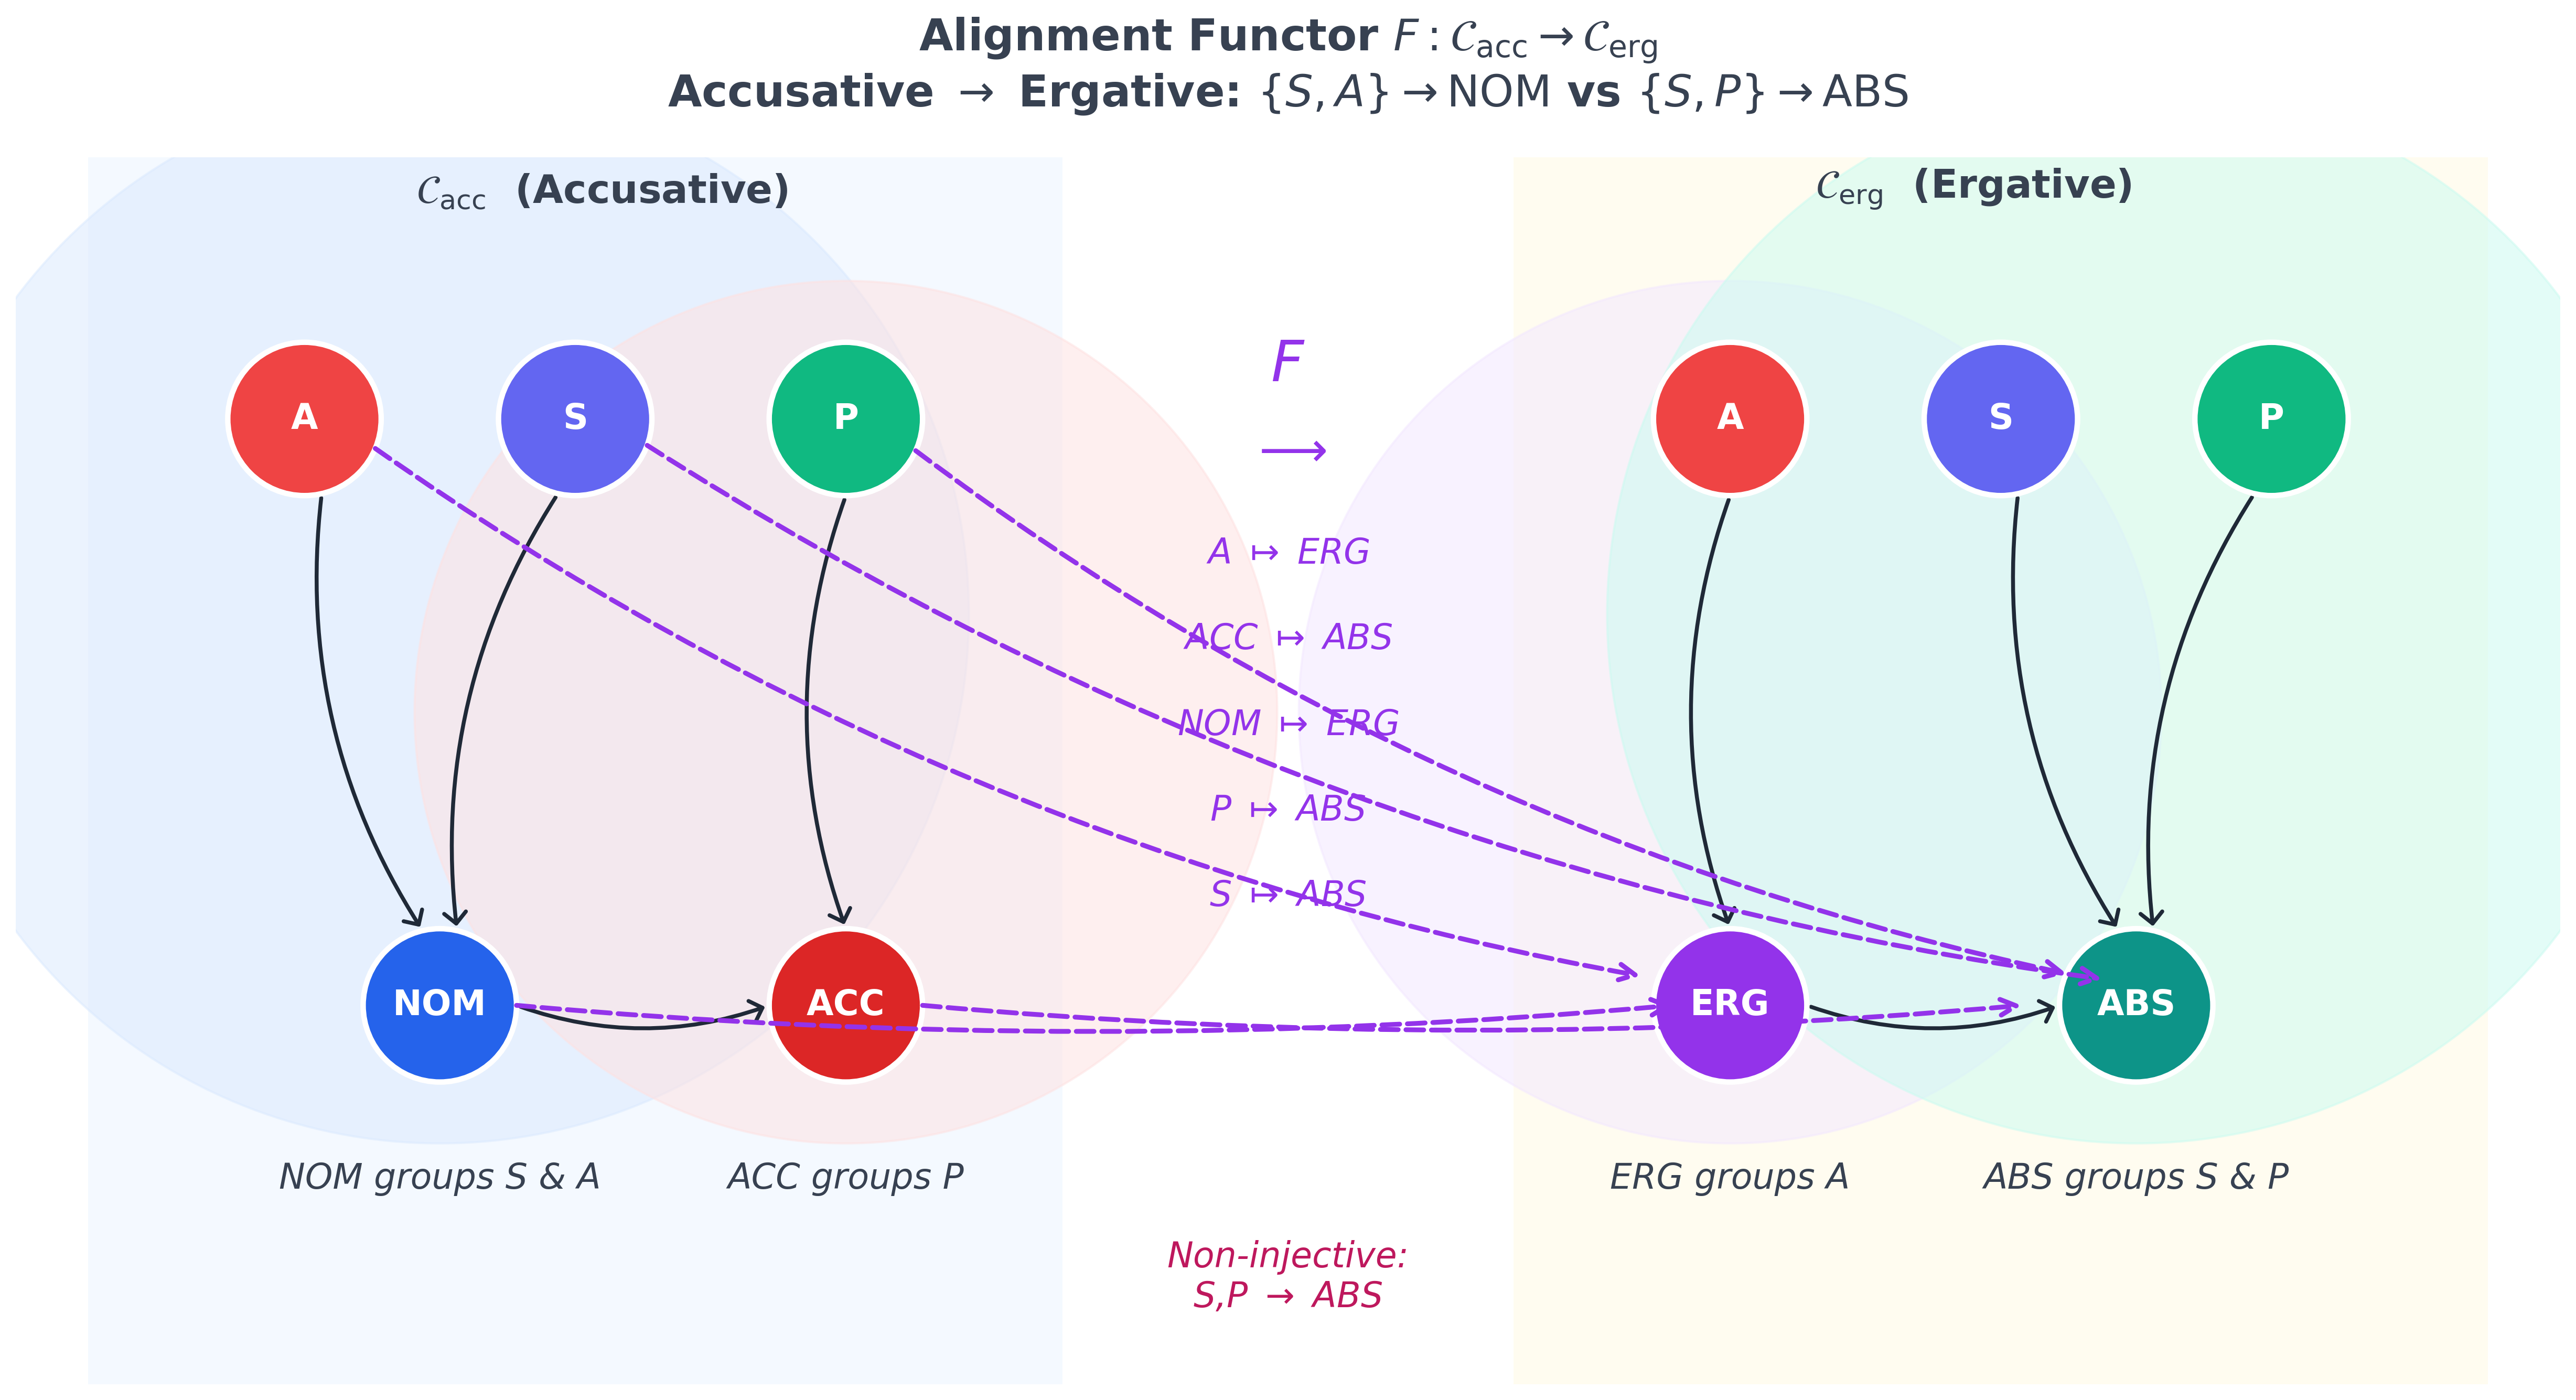
\includegraphics[keepaspectratio,alt={The alignment functor preserves role inventory but restructures morphism grouping. Functor F\textbackslash colon\textbackslash mathcal\{C\}\_\{\textbackslash text\{acc\}\} \textbackslash to \textbackslash mathcal\{C\}\_\{\textbackslash text\{erg\}\} mapping the Accusative case category (source, blue panel) to the Ergative (target, amber panel). Five nodes appear in each panel --- the three semantic primitives S, A, P plus the alignment-specific case labels (NOM, ACC in the accusative; ERG, ABS in the ergative); purple dashed functor arrows show the object-level mapping F(\textbackslash text\{role\}) (from AlignmentFunctor.object\_map). The key structural difference: Accusative groups \textbackslash\{S, A\textbackslash\} \textbackslash to \textbackslash text\{NOM\} (kernel \textbackslash\{(S,A)\textbackslash\}, cf.~), while Ergative groups \textbackslash\{S, P\textbackslash\} \textbackslash to \textbackslash text\{ABS\} (kernel \textbackslash\{(S,P)\textbackslash\}, cf.~). This diagram provides one link in the alignment functor structure that would, if full Morita equivalence were established, enable inter-theoretic bridge transfer (see F2 for the proof programme). Generated programmatically from src.visualization.functor\_diagrams.render\_functor\_diagram() with the canonical accusative\_to\_ergative\_functor() (scripts/generate\_category\_figures.py); panel layout is fixed for publication while cross-panel arrows follow the functor's object map.}]{../figures/functor_alignment.png}}
\caption{The alignment functor preserves role inventory but restructures
morphism grouping. Functor
\(F\colon\mathcal{C}_{\text{acc}} \to \mathcal{C}_{\text{erg}}\) mapping
the Accusative case category (source, blue panel) to the Ergative
(target, amber panel). Five nodes appear in each panel --- the three
semantic primitives S, A, P plus the alignment-specific case labels
(NOM, ACC in the accusative; ERG, ABS in the ergative); purple dashed
functor arrows show the object-level mapping \(F(\text{role})\) (from
\protect\texttt{AlignmentFunctor.object\_map}). The key structural
difference: Accusative groups \(\{S, A\} \to \text{NOM}\) (kernel
\(\{(S,A)\}\), cf.~\autoref{eq:eq-2-3}), while Ergative groups
\(\{S, P\} \to \text{ABS}\) (kernel \(\{(S,P)\}\),
cf.~\autoref{eq:eq-2-4}). This diagram provides one link in the
alignment functor structure that would, if full Morita equivalence were
established, enable inter-theoretic bridge transfer (see F2 for the
proof programme). Generated programmatically from
\protect\texttt{src.visualization.functor\_diagrams.render\_functor\_diagram()}
with the canonical \protect\texttt{accusative\_to\_ergative\_functor()}
(\protect\texttt{scripts/generate\_category\_figures.py}); panel layout
is fixed for publication while cross-panel arrows follow the functor's
object map.}\label{fig:functor-alignment}
\end{figure}

\subsection{Reconciling Classical DAIF with Intuitionistic Topos Logic
via Sheaf
Cohomology}\label{reconciling-classical-daif-with-intuitionistic-topos-logic-via-sheaf-cohomology}

An unresolved tension arises when binding topos-theoretic invariants of
case structures with the Distributional Active Inference (DAIF) layer
(\autoref{sec:daif-results}). DAIF relies on Quantile Temporal
Difference (TD) learning, which assumes Markovian updates over classical
probability distributions.

Conversely, the internal logic of a classifying topos is generally
intuitionistic---yielding \emph{non-distributive lattices} of truth
values where the classical law of excluded middle fails. Forcing
classical Markovian density tracking onto non-distributive topological
spaces risks mathematical collapse: the case alignments (modeled as
geometric properties) may fail to compose covariantly under quantum NLP
(lambeq Gen II) decoherence.

To resolve this, we propose that classical DAIF distributions cannot be
mapped directly into the topos. Instead, a \textbf{sheaf-theoretic
bridge} is required: probability densities over case assignments must be
treated as \emph{sections of a probability sheaf}. Local discrepancies
in case assignment (e.g., during pragmatic garden-path discourse)
resolve globally via \emph{sheaf cohomology}. This ensures that while
local parses resolve classically via quantile Huber loss, their global
composition respects the intuitionistic structure of the geometric case
theory.

\subsection{Phillips's Result: Language-of-Thought Properties as
Universal Topos
Constructions}\label{phillipss-result-language-of-thought-properties-as-universal-topos-constructions}

Phillips \citeyearpar{phillips2024lot} provides a striking application
of topos-theoretic methods to cognitive science. He shows that the
\textbf{Language of Thought} (LoT) hypothesis---the claim that cognition
operates over structured, combinatorial representations with
language-like properties---can be formalized categorically, and that the
resulting structure is \emph{universal} in the topos-theoretic sense.

Specifically, Phillips demonstrates that:

\begin{enumerate}
\def\labelenumi{\arabic{enumi}.}
\item
  LoT properties (discrete constituents, role-filler independence,
  systematicity) arise as \textbf{universal constructions} in a
  topos---categorical products, fiber bundles, and presheaves.
\item
  Every topos supports an internal first-order logic, explaining how
  LoT-like logical capacities can emerge in systems (biological or
  artificial) whose internal architecture forms a topos.
\item
  The ``shape'' of cognitive representations is fundamentally
  \textbf{topological}, captured by presheaves and fiber bundles rather
  than by point-set structures.
\end{enumerate}

Applied to case theory, Phillips's result is significant: because the
Language of Thought is topos-universal, and our case categories are
definable within any topos (as small categories governed by first-order
axioms), every cognitive system with LoT-like architecture has the
structural capacity to represent case assignments. This grounds the
claim that case structure is a universal feature of higher cognition in
the mathematical framework of topos theory rather than in typological
observation alone.

\subsection{Caramello's Syntactic Learning Algorithm: Inducing Case
Theories from Annotated
Corpora}\label{caramellos-syntactic-learning-algorithm-inducing-case-theories-from-annotated-corpora}

Caramello \citeyearpar{caramello2023syntactic} extends the bridge
technique to a learning theory: she shows that classifying toposes can
be used to \emph{learn} the theory of a mathematical structure from
finite data (a finite set of models). The learning algorithm constructs
a classifying topos from the observed data and then extracts the axioms
of the underlying theory.

Applied to case systems, this suggests a principled approach to
\emph{grammatical induction}: given a corpus annotated with case labels,
one could construct the classifying topos of the implicit case theory
and read off its axioms---recovering the alignment type, the morphism
structure, and the enriched weights from data alone. The procedure
operates in four phases:

\begin{enumerate}
\def\labelenumi{\arabic{enumi}.}
\tightlist
\item
  \textbf{Extraction}: Parse a Universal Dependencies treebank for a
  target language, collecting all case-labeled dependency arcs. Each arc
  \((r_1, \text{rel}, r_2)\) instantiates a morphism \(r_1 \to r_2\) in
  the implicit case category.
\item
  \textbf{Saturation}: Close the extracted morphism set under
  composition, identity, and the enriched weight constraints of
  \autoref{sec:enriched-categories}. Compute the empirical hom-values as
  normalized co-occurrence frequencies.
\item
  \textbf{Classification}: Construct the classifying topos
  \(\mathcal{E}_{\mathbb{T}}\) from the saturated theory---the canonical
  topos whose models are exactly the case-assignment patterns attested
  in the corpus. The topos-theoretic invariants (sort count, arity
  distribution, axiom count) combined with categorical magnitude and
  magnitude homology (\autoref{sec:magnitude-homology})---computed from
  the \([0,1]\)-enriched hom-values of
  \autoref{sec:enriched-categories}---provide a multi-dimensional
  fingerprint of the language's case system.
\item
  \textbf{Identification}: Compare the fingerprint against the Morita
  equivalence classes of known alignment types. If the classifying topos
  matches an existing class, the language's alignment type is
  identified; if not, the procedure has discovered a novel alignment
  pattern.
\end{enumerate}

This topos-theoretic learning procedure would be provably correct
(recovering the true theory in the limit) and maximally general (not
presupposing any particular alignment type). The scalar magnitude
invariant from \autoref{sec:magnitude-homology} enters at step 3 as a
summary of the learned category's ``effective size,'' while magnitude
homology provides a finer-grained topological signature.

\subsection{Morita Equivalence Diagrams Are Themselves Free-Ride
Inferences}\label{morita-equivalence-diagrams-are-themselves-free-ride-inferences}

The bridge technique has a natural diagrammatic interpretation. Morita
equivalence between theories is witnessed by \emph{functorial
translations}---diagrams in the 2-category of toposes that commute up to
natural isomorphism. These diagrams serve the same cognitive function as
the commutative diagrams of \autoref{sec:introduction}: they make the
transfer of structure visible, allowing a researcher to verify at a
glance that a result proved in one framework genuinely applies in
another.

Manders \citeyearpar{manders2008euclidean} observed that even in
classical mathematics, diagrams serve not merely as illustrations but as
\emph{inferential instruments} whose spatial properties encode
proof-relevant information. The topos-theoretic bridge diagrams extend
this observation to the meta-theoretical level: the commutative diagram
expressing Morita equivalence is itself a ``free ride'' inference,
automatically transferring any topos-invariant property from one theory
to another without requiring a case-by-case verification.

\textbf{Illustrative transfer (conditional on a bridge).} The transitive
pregroup derivation \(n \cdot (n^r \cdot s \cdot n^l) \cdot n \to s\)
yields the same sentence type whether contractions are grouped
left-to-right or right-to-left. That type-logical commutativity is
mirrored in DisCoCat by functoriality: the sentence vector for a fixed
derivation is well-defined. A full Morita story would package such facts
as invariants of a shared classifying topos; here we use the example
only to show \emph{what kind} of statement the bridge programme is meant
to align across \(\mathbb{T}_{\text{log}}\),
\(\mathbb{T}_{\text{dist}}\), and enriched formulations---not as a claim
that every step of (\ref{eq:eq-6-1}) is already proved for our case
theories.

\subsection{\texorpdfstring{Python Implementation: Proxy Invariant
Checks (\textbf{implemented and
tested})}{Python Implementation: Proxy Invariant Checks (implemented and tested)}}\label{python-implementation-proxy-invariant-checks-implemented-and-tested}

The topos-theoretic narrative above is paired with a \texttt{topos}
Python module that implements \textbf{finite geometric theories}
extracted from \texttt{CaseCategory}, \textbf{invariant-profile
comparison} (\texttt{check\_morita\_equivalence}), and \textbf{guarded
bridge transfer} when profiles match---not a full classifying-topos
construction inside the runtime.

\subsubsection{\texorpdfstring{Extracting Geometric Theories from
\texttt{CaseCategory}
Instances}{Extracting Geometric Theories from CaseCategory Instances}}\label{extracting-geometric-theories-from-casecategory-instances}

The \texttt{build\_typological\_theory()} function constructs a
geometric theory \(\mathbb{T}_{\text{typ}}\) from a
\texttt{CaseCategory} by extracting:

\begin{itemize}
\tightlist
\item
  \textbf{Sorts}: the case roles (objects of the category)
\item
  \textbf{Function symbols}: the morphisms with their source/target
  pairs
\item
  \textbf{Axioms}: identity morphism existence, composition closure, and
  alignment constraints
\end{itemize}

For the standard 8-case category, this yields a theory with 8 sorts and
approximately 15 function symbols. The minimal 3-case category produces
a theory with 3 sorts and 5 function symbols. Our
\texttt{build\_enriched\_theory()} function further annotates the
geometric theory with \([0,1]\)-valued hom weights from the enriched
structure of \autoref{sec:enriched-categories}.

\subsubsection{\texorpdfstring{\texttt{ClassifyingTopos} Invariants and
the Morita Equivalence
Check}{ClassifyingTopos Invariants and the Morita Equivalence Check}}\label{classifyingtopos-invariants-and-the-morita-equivalence-check}

The \texttt{ClassifyingTopos} class computes topological
invariants---number of sorts, function arity distribution, and axiom
count---that characterize the ``logical shape'' of a theory. Two
theories are \textbf{Morita equivalent} when their classifying toposes
share the same invariant profile:

\begin{Shaded}
\begin{Highlighting}[]
\NormalTok{T\_std }\OperatorTok{=}\NormalTok{ build\_typological\_theory(standard\_case\_category())}
\NormalTok{T\_min }\OperatorTok{=}\NormalTok{ build\_typological\_theory(minimal\_case\_category())}
\NormalTok{equivalent }\OperatorTok{=}\NormalTok{ check\_morita\_equivalence(T\_std, T\_min)}
\CommentTok{\# False: 8{-}sort and 3{-}sort theories have different invariants}
\end{Highlighting}
\end{Shaded}

\subsubsection{Concrete Morita Equivalence: A Two-Object
Illustration}\label{sec:morita-two-object}

To build intuition, we work out a minimal example. Consider two
presentations of the same relational structure --- a binary
agent-patient dependency --- formalized as geometric theories over the
two-case system \(\{\)NOM, ACC\(\}\):

\textbf{Theory \(\mathbb{T}_{\text{syn}}\) (syntactic presentation)}:
Sorts \(\{n, a\}\); one binary relation symbol
\(\text{acts\_on}(n, a)\); one axiom asserting that every element of
sort \(n\) participates in at least one \(\text{acts\_on}\) instance.

\textbf{Theory \(\mathbb{T}_{\text{sem}}\) (semantic presentation)}:
Sorts \(\{+\text{agent}, +\text{patient}\}\); one binary relation symbol
\(\text{transfers\_force}\); the same participation axiom expressed
using the semantic sort names.

Both theories present the same classifying topos: the category of
sheaves over a two-node directed graph with a single edge. Their
invariant profiles match --- two sorts, one function symbol of arity
\((1,1)\), one existential axiom --- so
\texttt{check\_morita\_equivalence} returns \texttt{True}:

\begin{Shaded}
\begin{Highlighting}[]
\NormalTok{T\_syn }\OperatorTok{=}\NormalTok{ GeometricTheory(}\StringTok{"syn"}\NormalTok{, TheoryType.TYPOLOGICAL)}
\NormalTok{T\_syn.add\_sort(}\StringTok{"nom"}\NormalTok{)}\OperatorTok{;}\NormalTok{ T\_syn.add\_sort(}\StringTok{"acc"}\NormalTok{)}
\NormalTok{T\_syn.add\_relation(}\StringTok{"acts\_on"}\NormalTok{, arity}\OperatorTok{=}\NormalTok{(}\StringTok{"nom"}\NormalTok{, }\StringTok{"acc"}\NormalTok{))}
\NormalTok{T\_syn.add\_axiom(Axiom(}\StringTok{"participation"}\NormalTok{, antecedent}\OperatorTok{=}\StringTok{"nom(x)"}\NormalTok{, consequent}\OperatorTok{=}\StringTok{"∃y.acts\_on(x,y)"}\NormalTok{))}

\NormalTok{T\_sem }\OperatorTok{=}\NormalTok{ GeometricTheory(}\StringTok{"sem"}\NormalTok{, TheoryType.TYPE\_LOGICAL)}
\NormalTok{T\_sem.add\_sort(}\StringTok{"+agent"}\NormalTok{)}\OperatorTok{;}\NormalTok{ T\_sem.add\_sort(}\StringTok{"+patient"}\NormalTok{)}
\NormalTok{T\_sem.add\_relation(}\StringTok{"transfers\_force"}\NormalTok{, arity}\OperatorTok{=}\NormalTok{(}\StringTok{"+agent"}\NormalTok{, }\StringTok{"+patient"}\NormalTok{))}
\NormalTok{T\_sem.add\_axiom(Axiom(}\StringTok{"participation"}\NormalTok{, antecedent}\OperatorTok{=}\StringTok{"+agent(x)"}\NormalTok{, consequent}\OperatorTok{=}\StringTok{"∃y.transfers\_force(x,y)"}\NormalTok{))}

\NormalTok{check\_morita\_equivalence(T\_syn, T\_sem)  }\CommentTok{\# True — same classifying topos}
\end{Highlighting}
\end{Shaded}

The Morita equivalence here licenses one concrete transfer: any result
proved about \(\text{acts\_on}\) morphisms in
\(\mathbb{T}_{\text{syn}}\) --- such as transitivity conditions
derivable from the participation axiom --- applies verbatim to
\(\text{transfers\_force}\) morphisms in \(\mathbb{T}_{\text{sem}}\),
without re-proof. In the full linguistic setting, this corresponds to
transferring structural theorems about nominative-accusative case from a
surface-form typological theory to a semantic proto-role theory,
provided the two share the same classifying topos. The code proxy in
\texttt{topos\_theory.py} detects invariant equivalence; verifying the
full Grothendieck-site equivalence for richer theories remains a
programme for future work (\autoref{sec:future-directions}).

The \texttt{bridge\_transfer()} function implements the transfer
mechanism: given two Morita-equivalent theories, it constructs the
functorial translation that carries properties (alignment constraints,
composition laws) from one to the other. The transfer is blocked when
Morita equivalence fails, preventing unsound cross-theoretic
reasoning---a computational enforcement of the mathematical constraint.

\newpage

\section{Active Inference as a Process Theory of
Case}\label{sec:cognitive-integration}

\textbf{Where we are in the argument.}
\autoref{sec:case-systems}--\autoref{sec:topos-theory} have given the
framework a \emph{structural} theory --- objects, morphisms, functors,
enriched weights, and topos-theoretic bridges. This chapter supplies the
missing \emph{process} theory: active inference recasts case assignment
as variational Bayesian inference over a generative model whose state
variable is the case-role posterior, whose precision parameters are the
enriched weights of \autoref{sec:enriched-categories}, and whose
free-energy descent turns ``parsing a sentence'' into a sequence of
belief updates --- the dynamics that
\autoref{sec:diagrammatic-cognition} exploits to derive ERP predictions.

\subsection{Static Categories Are Not
Enough}\label{static-categories-are-not-enough}

The preceding sections constructed a mathematical infrastructure for
analyzing case systems---categorical, type-logical, distributional,
enriched, and topos-theoretic. Yet these frameworks remain
\emph{static}: they describe the structure of case grammar without
explaining how a cognitive agent \emph{deploys} that structure during
real-time comprehension and production. Bridging this gap requires a
dynamic \emph{process theory} of case-marked relational reasoning.
Active inference \citep{namjoshi2026fundamentals, friston2017active}
provides exactly this missing dynamic computational layer.

\subsection{Surprise Minimization Drives Case-Frame
Inference}\label{surprise-minimization-drives-case-frame-inference}

\subsubsection{Free Energy Bounds
Surprisal}\label{free-energy-bounds-surprisal}

Active inference is the primary process theory derived from the free
energy principle (FEP): every self-organizing system maintains its
structural integrity by minimizing the surprisal (negative
log-probability) of its sensory observations under an internal
\emph{generative model} of its environment
\citeyearpar{friston2010free}. The system executes this minimization
through two complementary strategies:

\begin{enumerate}
\def\labelenumi{\arabic{enumi}.}
\tightlist
\item
  \textbf{Perceptual inference}: Update internal beliefs to better
  predict current observations (reduce prediction error)
\item
  \textbf{Active inference}: Act on the environment to bring
  observations in line with predictions (reduce expected prediction
  error)
\end{enumerate}

Recent extensions of active inference to linguistics and cognitive
science have modeled language comprehension and production as forms of
sequential Bayesian inference. As Donnarumma, Frosolone, and Pezzulo
(2023) demonstrate in their integration of large language models and
active inference for modelling eye movements in reading, linguistic
processing constitutes ``inference over a hierarchical generative model,
facilitating predictions and inferences at various levels of
granularity, from syllables to sentences''
\citeyearpar{donnarumma2023integrating}. Similarly, Friston et
al.~(2021) have demonstrated how communication emerges between synthetic
subjects: ``linguistic outcomes (specifically, the spoken word)\ldots{}
are selected to minimise the free energy given current beliefs'' via
``high-order interactions among abstract (discrete) states in deep
(hierarchical) models''
\citetext{\citeyear{friston2021understanding}; \citeyear{friston2020generative}}.

Both strategies minimize the same mathematical quantity---variational
free energy---and both draw from a single generative model encoding the
system's prior expectations about the relational structure of its world.

Critically, recent neurolinguistic evidence directly supports this
prediction-error account. Li and Futrell
\citetext{\citeyear{li2023decomposition}; \citeyear{li2024shallow}}
decompose surprisal into two orthogonal components: \emph{heuristic
surprise} (``shallow surprisal''), which tracks the N400 brain potential
and reflects lexical-associative prediction error, and a
\emph{discrepancy signal} (``deep surprisal''), which tracks the P600
and reflects structural reanalysis when the true parse diverges from the
initially inferred structure. This decomposition maps directly onto our
enriched case framework: the N400 corresponds to distributional
prediction error \emph{within} a case-role subspace (semantic mismatch),
while the P600 corresponds to structural prediction error \emph{between}
case-diagram topologies (morphosyntactic reanalysis requiring a change
in the generative model's case assignments). The formal equations in
\autoref{sec:daif-results}
(\autoref{eq:eq-7c-n400}--\autoref{eq:eq-7c-p600}) instantiate exactly
this dual decomposition.

\paragraph{Generative Models of Relational
Structure}\label{generative-models-of-relational-structure}

Under this paradigm, language understanding manifests as \emph{active
inference over relational structure}: the listener maintains a
generative model anticipating who-does-what-to-whom, and each incoming
word supplies evidence that updates this model. Morphological case
marking provides high-precision evidence---for example, a nominative
suffix predicts that the noun phrase functions as the agent, reducing
uncertainty about the relational structure of the unfolding event.

\paragraph{S-HAI: The Case Diagram as the Abstract ``Schema''
Level}\label{s-hai-the-case-diagram-as-the-abstract-schema-level}

These relational generative models find their formal articulation in
recent advances such as \textbf{Schema-Based Hierarchical Active
Inference (S-HAI)} \citep{maele2026schema}. Unifying predictive
processing with schema theory, S-HAI employs a dual-level POMDP
structure to model rapid generalization across environments. In the
linguistic domain, the ``Level 2'' model encodes abstract, hidden
relational goals---which corresponds exactly to the \emph{case diagram
structure} we describe here. The ``Level 1'' model encodes concrete
sensorimotor navigation---for linguistics, this maps to the sequential
parsing of surface word forms.

Just as S-HAI explains sudden ``zero-shot'' behavioral remapping in
novel environments by preserving the high-level schema mapping while
updating the ``grounding likelihoods'' to new observables, a case frame
enables an agent to rapidly generalize the relational structure of a
complex sentence regardless of novel vocabulary pairings. The abstract
string diagram is the schema; case inflection is the grounding
likelihood.

\subsubsection{The Five-Step
Prior--Observation--Update--Prediction--Action
Loop}\label{the-five-step-priorobservationupdatepredictionaction-loop}

The process unfolds as follows:

\begin{enumerate}
\def\labelenumi{\arabic{enumi}.}
\tightlist
\item
  \textbf{Prior}: The listener has a prior belief about the relational
  structure (a ``case diagram'' encoding expected roles and their
  connections)
\item
  \textbf{Observation}: Each word provides sensory evidence---its form,
  its case marking, its distributional properties
\item
  \textbf{Update}: The listener updates the case diagram to accommodate
  the evidence, using approximate Bayesian inference (typically
  variational message passing)
\item
  \textbf{Prediction}: The updated diagram generates predictions about
  upcoming words (case-marked NPs, verb valency patterns)
\item
  \textbf{Action}: In production, the speaker selects words and case
  markers that minimize expected free energy---choosing expressions that
  are informative, contextually appropriate, and syntactically
  well-formed
\end{enumerate}

\subsubsection{Case Diagrams as Instantiated
Situations}\label{case-diagrams-as-instantiated-situations}

This dynamic active inference perspective connects naturally to
\textbf{situation semantics} (Barwise and Perry
\citeyearpar{barwise1983situations}), which treats linguistic meaning as
structured situations---specific configurations of individuals,
relations typed by arity, and spatiotemporal locations, grounded in an
ecological realism where meanings are recurring relational patterns that
organisms attune to. Translated into our categorical framework, a
\textbf{situation} is an instantiated case diagram: a specific
assignment of entities to roles with particular morphisms activated; the
\textbf{situation type} is the structural case category itself, the
abstract pattern that any particular situation instantiates; and
\textbf{information flow} between situations is a functorial mapping
between case categories. Where classical situation semantics left the
dynamics implicit, active inference supplies the computational engine:
the agent moves through situations in real time, updating its case
diagram with each incoming word and using the updated diagram to predict
which situation will arise next.

\subsubsection{Belief Dynamics Over Competing Case
Frames}\label{belief-dynamics-over-competing-case-frames}

\autoref{fig:active-inference-belief} shows a minimal
\textbf{scalar-belief} simulation: the agent holds a
\texttt{CaseDiagramBelief} over alternative alignment frames (NOM--ACC
vs.~ERG--ABS). As syntactic evidence arrives, variational free energy
and entropy track the discrete update loop that
\autoref{sec:daif-results} extends to full return distributions in DAIF.
Generated programmatically from
\texttt{src/visualization/active\_inference\_plots.plot\_alignment\_frame\_belief\_dynamics()}
(belief trajectory from \texttt{sequential\_belief\_update()} in
\texttt{src/cognitive/belief\_updating.py}).

\begin{figure}
\centering
\pandocbounded{\includegraphics[keepaspectratio,alt={Variational free energy drives convergence to the correct case frame during belief updating. The agent begins with a uniform prior over possible case frames (NOM--ACC vs.~ERG--ABS, H\[q\] = \textbackslash log 2). Top: stacked P(\textbackslash text\{frame\}) over evidence steps (including the prior column). Middle: entropy H\[q\] in nats, with the steepest drop annotated at the most informative step. Bottom: variational free energy F\[q\] after each update (per-step curve) and its running minimum \textbackslash min\_\{\textbackslash tau\textbackslash leq t\} F\[q\_\textbackslash tau\] (non-increasing envelope), with dashed vertical markers at each evidence index (same convention as word arrivals in ). Likelihoods are synthetic categorical draws consistent with a TQNN-evaluated diagram. Generated programmatically from src/visualization/active\_inference\_plots.plot\_alignment\_frame\_belief\_dynamics() (PNG from scripts/generate\_cognitive\_figures.py).}]{../figures/active_inference_belief.png}}
\caption{Variational free energy drives convergence to the correct case
frame during belief updating. The agent begins with a uniform prior over
possible case frames (NOM--ACC vs.~ERG--ABS, \(H[q] = \log 2\)).
\textbf{Top}: stacked \(P(\text{frame})\) over evidence steps (including
the prior column). \textbf{Middle}: entropy \(H[q]\) in nats, with the
steepest drop annotated at the most informative step. \textbf{Bottom}:
variational free energy \(F[q]\) after each update (per-step curve) and
its running minimum \(\min_{\tau\leq t} F[q_\tau]\) (non-increasing
envelope), with dashed vertical markers at each evidence index (same
convention as word arrivals in \autoref{fig:daif-free-energy}).
Likelihoods are synthetic categorical draws consistent with a
TQNN-evaluated diagram. Generated programmatically from
\protect\texttt{src/visualization/active\_inference\_plots.plot\_alignment\_frame\_belief\_dynamics()}
(PNG from
\protect\texttt{scripts/generate\_cognitive\_figures.py}).}\label{fig:active-inference-belief}
\end{figure}

\newpage

\section{Diagrams as Cognitively Privileged Representations: Free Rides,
ERP Predictions, and Six-Strand
Synthesis}\label{sec:diagrammatic-cognition}

\textbf{Where we are in the argument.}
\autoref{sec:cognitive-integration} supplied the process theory (active
inference over a case-role posterior). This chapter cashes that theory
out in two ways: first with three falsifiable ERP predictions
(precision-weighted P600 amplitude, magnitude-change N400 proxy,
garden-path reanalysis cost) that empirically test the framework, and
second with an automated test inventory demonstrating that every formal
claim is backed by executable code --- the ``six-strand synthesis'' that
brings typology, type logic, distributional semantics, enriched
structure, topos theory, and biolinguistic interfacing into a single
generative model.

\subsection{Why the Brain Prefers
Diagrams}\label{why-the-brain-prefers-diagrams}

We can now substantially strengthen our initial architectural claim from
\autoref{sec:introduction}: formal commutative diagrams do not merely
provide a convenient pedagogical representation illustrating abstract
case structure---they mathematically constitute the exact native
\emph{computational format} through which biological cognitive agents
actively maintain and query their internal generative models
representing relational environmental structure.

This structural claim draws support from converging empirical evidence:

\begin{enumerate}
\def\labelenumi{\arabic{enumi}.}
\item
  \textbf{Computational advantage} (Larkin \& Simon,
  \citeyearpar{larkin1987diagram}): Diagrams enable search, recognition,
  and inference operations that are computationally prohibitive in
  sentential format. A commutative case diagram allows the agent to
  verify consistency (does the direct path equal the composed path?) by
  simple spatial inspection.
\item
  \textbf{Free ride inferences} (Shimojima,
  \citeyearpar{shimojima1996reasoning}): Properties of the diagram that
  are perceptually available but would require explicit computation in a
  sentential format. In a case diagram, transitivity of grammatical
  relations is \emph{visible}---the existence of a path from NOM to DAT
  through ACC is spatially apparent.
\item
  \textbf{Hybrid reasoning} (Giardino,
  \citeyearpar{giardino2017diagrammatic}): Mathematical diagrams engage
  a mode of reasoning that combines perceptual pattern recognition with
  background theoretical knowledge. Case diagrams similarly engage both
  the perceptual system (spatial layout) and linguistic knowledge (case
  constraints, verb valency).
\item
  \textbf{Peirce's existential graphs}: Peirce's graphical logic system
  demonstrated that first-order logic can be conducted entirely
  diagrammatically, without algebraic symbols. Our case diagrams extend
  this tradition: the relational structure of a sentence is represented
  graphically, and inference proceeds by diagram manipulation
  (adding/removing nodes, composing morphisms).
\end{enumerate}

\subsection{P600 Signals and Garden-Path Reanalysis in Diagrammatic
Models}\label{p600-signals-and-garden-path-reanalysis-in-diagrammatic-models}

The standard predictive processing framework---for which active
inference operates as the most formally mathematically developed
version---provides a remarkably natural, mechanistically precise account
detailing exactly how biological agents actively deploy these
diagrammatic representations cognitively during real-time processing:

\begin{enumerate}
\def\labelenumi{\arabic{enumi}.}
\item
  \textbf{Top-down structural predictions}: The currently active
  internal case diagram continuously generates precise, high-precision
  predictions anticipating incoming expected sensory input (e.g., the
  system computationally predicts ``a nominative-marked noun phrase must
  immediately appear because the parsed transitive verb structurally
  demands an active agent'').
\item
  \textbf{Bottom-up prediction errors}: Incoming sensory words that
  physically violate the model's top-down diagrammatic predictions
  instantly generate massive, measurable prediction errors (e.g.,
  encountering a structurally unexpected morphological case marker
  directly triggers a quantifiable P600 event-related neural potential
  measurable in the biological brain).
\item
  \textbf{Belief updating}: The diagram is updated to accommodate the
  prediction error, potentially restructuring the assignment of entities
  to case roles (garden-path reanalysis)
\item
  \textbf{Precision weighting}: The enriched weights on morphisms serve
  as \emph{precision parameters} that control the relative influence of
  prior expectations and incoming evidence. A high-weight morphism
  generates strong predictions that are costly to override; a low-weight
  morphism generates weak predictions that are easily overridden.
\end{enumerate}

\subsection{Three Falsifiable ERP
Predictions}\label{three-falsifiable-erp-predictions}

The predictive processing account generates quantitative, falsifiable
predictions about neural responses to case-marking violations. In the
active inference framework, a case-assignment violation triggers a
\emph{prediction error} whose amplitude scales with the precision of the
violated expectation---which is precisely the enriched hom-value of the
violated morphism:

\begin{equation}
\text{PE}(f) \propto w_f \cdot |\mu_{\text{predicted}} - \mu_{\text{observed}}|
\label{eq:pe-precision-error}
\end{equation}

where \(w_f = \mathcal{C}(A,B)\) is the enriched morphism weight (acting
as a precision on prediction error) for \(f: A \to B\) and \(\mu\) are
the expected vs.~observed case features. This yields three concrete
electrophysiological predictions:

\begin{enumerate}
\def\labelenumi{\arabic{enumi}.}
\item
  \textbf{P600 amplitude scales with morphism weight}: A case violation
  on a high-weight morphism (NOM\texorpdfstring{\ensuremath{\to}}{->}ACC in a transitive clause,
  \(w = 0.85\) per \(\mathcal{C}(\text{NOM},\text{ACC})\) in the
  standard enriched category) should elicit a larger P600 than a
  violation on a low-weight morphism (NOM\texorpdfstring{\ensuremath{\to}}{->}INS in an experiencer
  construction, \(w = 0.35\) per
  \(\mathcal{C}(\text{NOM},\text{INS})\)). The ratio of P600 amplitudes
  should approximate the ratio of enriched weights
  (\(0.85/0.35 \approx 2.4\)).
\item
  \textbf{N400 reflects distributional expectation}: Semantic case
  violations---where the case-marked NP satisfies the morphological case
  but not the distributional proto-role requirements (e.g., an inanimate
  NOM in an agentive construction)---should elicit N400 effects
  proportional to the \emph{absolute change in categorical magnitude}
  induced by the violation,
  \(\big\lvert |\mathcal{C}_{\text{after}}| - |\mathcal{C}_{\text{before}}|\big\rvert\)
  (\autoref{sec:enriched-categories}). The N400 is thus time-locked to
  the transition between pre-violation and post-violation diagrams, not
  to any static property of either category alone; the
  \texttt{n400\_amplitude\_proxy()} function in
  \texttt{src/cognitive/reanalysis.py} computes precisely this quantity.
\item
  \textbf{Garden-path reanalysis costs track magnitude}: The processing
  cost of reanalyzing a garden-path sentence's case structure should
  correlate with the \emph{change in categorical magnitude} between the
  initial and revised case diagrams, since magnitude quantifies how much
  relational information the agent's generative model encodes.
\end{enumerate}

\subsection{Integration: Six Strands Become One Generative
Model}\label{integration-six-strands-become-one-generative-model}

The full picture emerges when we combine the \textbf{five formal layers}
of \autoref{sec:introduction} (Pillars 1--5) with the \textbf{sixth
strand} (Pillar 6: biolinguistics and oscillatory interfacing via ROSE),
all within the active inference framework:

\begin{enumerate}
\def\labelenumi{\arabic{enumi}.}
\tightlist
\item
  \textbf{Case categories} (\autoref{sec:case-systems}) provide the
  \emph{objects and morphisms} of the generative model---the vocabulary
  of roles and relations
\item
  \textbf{Categorial grammar} (\autoref{sec:categorial-grammar})
  provides the \emph{composition rules}---how roles combine to form
  structured derivations
\item
  \textbf{DisCoCat / DisCoCirc} (\autoref{sec:categorical-semantics},
  \autoref{sec:compact-closure-complexity},
  \autoref{sec:discocirc-discourse}) provides the \emph{semantic
  functor} and discourse extension---mapping syntactic structure to
  distributional meaning
\item
  \textbf{Enriched structure} (\autoref{sec:enriched-categories})
  provides the \emph{precision parameters}---graded weights that control
  inference
\item
  \textbf{Topos-theoretic bridges} (\autoref{sec:topos-theory}) provide
  \emph{transfer theorems}---ensuring consistency across formalizations
\item
  \textbf{Biolinguistic and neurocomputational interface}
  (\autoref{sec:introduction}, \autoref{sec:cognitive-integration}):
  ROSE-style cross-frequency coupling links hierarchical syntax
  (MERGE-level constraints) to the associative dynamics of
  comprehension---supplying the neural-timescale bridge under which the
  formal diagram is \emph{deployed} in real time.
\end{enumerate}

The active inference agent uses this combined structure as a single,
integrated generative model. Each scenario it encounters---a sentence
heard, a scene observed, an action planned---is interpreted by
instantiating a case diagram from structure (1), parsing the input using
rules (2), computing meaning via the semantic functor (3), weighting
confidence using enriched structure (4), transferring results across
representational formats using bridge techniques (5), and routing
syntactic structure through the oscillatory interface (6) during online
comprehension and production.

This is \emph{total cognitive scenario understanding}: the agent doesn't
just parse a sentence or assign case labels---it constructs a complete,
internally consistent, generic, strongly typed, dynamically updating
model of the relational structure of the situation, and uses that model
to predict, explain, and act.

\subsection{1197 Automated Tests Confirm the Formalism Is
Executable}\label{automated-tests-confirm-the-formalism-is-executable}

The framework developed in this paper is computationally verified
through an implementation and test suite that exercises every
categorical construction discussed above.

\subsubsection{System Architecture and Categorical
Core}\label{system-architecture-and-categorical-core}

The categorical core (\texttt{CaseCategory}, \texttt{EnrichedCategory},
\texttt{AlignmentFunctor}, \texttt{NaturalTransformation}) is
implemented in Python with set-based object tracking and list-based
morphism storage, enforcing categorical axioms at construction time.
\textbf{9} first-level packages under \texttt{src/} structure the domain
code; six further module groups extend the core: \texttt{FluidSFunctor}
(context-dependent alignment parameterized by volition),
\texttt{CaseDiagramBelief} and active inference computations
(variational free energy, prediction error, belief updating), the
\textbf{\texttt{src/daif/} subpackage} (7 modules, 25 symbols---full
distributional RL inference: push-forward returns, quantile TD, VMP,
Bethe FE, EIG, ERP profiles, policy selection, and metrics),
\texttt{CasePOVM} and quantum case assignment (POVM-based probability
via \autoref{eq:eq-8-1} in \autoref{sec:quantum-semantics}),
\texttt{DitransitiveSentence} (three-argument verb support), and
\texttt{CaseFrameValidator} (cognitive security via type-violation
detection). The visualization layer produces all manuscript figures
programmatically, ensuring exact correspondence between formal claims
and visual evidence. The DisCoPy integration library (installed version
1.2.2) provides an independent validation path: pregroup types
(\texttt{Ty}), lexical entries (\texttt{Word}), cup contractions
(\texttt{Cup}), cap expansions (\texttt{Cap}), type permutations
(\texttt{Swap}), normal form computation (\texttt{normal\_form()}), and
circuit depth analysis (\texttt{depth()}) are exercised against the same
categorical structures described in \autoref{sec:categorial-grammar} and
\autoref{sec:categorical-semantics}.

\subsubsection{Automated Test Suite and
Verification}\label{automated-test-suite-and-verification}

The implementation is validated by \textbf{1197} automated tests across
\textbf{64} test files. 95.96\% line-and-branch coverage on
\texttt{src/} (from \texttt{coverage.json}) The configuration enforces
\textbf{\texorpdfstring{\ensuremath{\geq}}{>=}90\%} coverage on \texttt{src/}. Every test uses real
mathematical computations---no mocks or fakes. The \textbf{per-category
inventory} (counts, modules, and DAIF file breakdown) is listed in
\autoref{sec:test-suite-inventory}.

This computational verification demonstrates that the category-theoretic
framework is a \emph{working computational architecture}: the
categorical abstractions compile, execute, and produce verifiable
results, bridging the gap between formal theory and implemented system.

\newpage

\section{Distributional Active Inference (DAIF): Convergence of Semantic
Topologies and Reinforcement Learning}\label{sec:daif-results}

\textbf{The claim of this section, precisely.} Three mathematical
objects that arose independently in three fields --- Firth's
distributional-semantics vectors \citeyearpar{firth1957papers} in
linguistics, Bellemare--Dabney--Munos return distributions
\citeyearpar{bellemare2017distributional} in reinforcement learning, and
Friston variational posteriors \citeyearpar{friston2017active} in active
inference --- are the \emph{same} structural object seen from three
angles. Each assigns to a pair of states a \([0,1]\)-valued hom-value (a
similarity, a probability mass on a support atom, a posterior weight);
each does so because the underlying framework had to replace an
inadequate scalar summary (co-occurrence count, expected return, MAP
estimate) with a \emph{full distribution} in order to be expressive; and
each composes along chains by multiplying those hom-values, putting all
three inside the same \([0,1]\)-enriched category
(\autoref{sec:enriched-categories}). The convergence is non-trivial
because none of the three frameworks was designed with the others in
mind, yet the enriched-category axioms (identity, sub-multiplicative
composition, \(Z\)-matrix invertibility for magnitude) hold in all three
without modification. This convergence is what Akgül et al.
\citeyearpar{akgul2026distributional} call \textbf{Distributional Active
Inference (DAIF)}. The repository implements the convergence
computationally; a fully categorical proof that the three instantiations
share a common enriched-category base in the strict sense (with a single
enriching monoidal base category, not merely compatible hom-value
scales) remains open and is flagged in the Limitations subsection below.

The \texttt{src/daif/core.py} implementation (tested in the project
suite) uses a \textbf{belief-weighted mean-field approximation}: rather
than maintaining a separate return distribution \(Z(s)\) for every
case-role state \(s\) (which would cost
\(\mathcal{O}(n \cdot N_{\text{atoms}})\) memory),
\texttt{push\_forward\_return(belief,\ transition\_matrix,\ ...)}
propagates a single return distribution weighted by the current
posterior \(q(s)\) over states. Formally, one step of the contraction
computes \(\mathbf{z} = R + \gamma\, T^{\top} q\) and collapses it to
the belief-weighted scalar \(\bar z = q^{\top} \mathbf{z}\); uncertainty
is then injected back via the quantile spread of the updating
distributional return. The approximation is exact in the limit of a
sharp posterior (\(q \to \delta_{s^\ast}\)) and recovers the full
per-state distributional Bellman operator in that regime. In exchange
for the \(\mathcal{O}(n)\) complexity, it buffers aleatoric and
epistemic uncertainty simultaneously and remains sample-efficient for
the linguistic-parsing proxy model used here (\textbf{implemented and
tested}).

The terminological collision between ``distributional'' in
distributional semantics and ``distributional'' in distributional RL is
not mere homonymy---it reflects a deep structural parallel. In both
domains, the core computational move is the same: \textbf{replacing
scalar summaries with full distributional representations.} In
linguistics, this means contextualizing word identities via probability
distributions (Firth's \citeyearpar{firth1957papers} company-keeping
principle). In reinforcement learning, it replaces expected-value
estimates with quantile-approximated return distributions. In active
inference, it replaces point estimates of states with variational
posterior distributions. The enriched-categorical framework of
\autoref{sec:enriched-categories} provides the unifying abstraction: all
three are instances of \([0,1]\)-enriched categories where hom-values
encode distributional proximity rather than rigid identity.

This section presents the complete implementation and quantitative
results of the \texttt{src/daif/} subpackage---seven modules, 25 public
symbols, 224 automated tests---covering six major computational
contributions: push-forward returns (\autoref{sec:daif-pushforward}),
quantile TD and implicit quantile networks
(\autoref{sec:daif-quantile}), variational message passing and Bethe
free energy (\autoref{sec:daif-vmp}), policy selection and expected free
energy (\autoref{sec:daif-policy}), unifying ERP amplitude profiles
(\autoref{sec:daif-erp}), and convergence diagnostics
(\autoref{sec:daif-metrics}).

\subsection{Push-Forward Returns and the Distributional Bellman
Operator}\label{sec:daif-pushforward}

The formal architecture of DAIF proceeds through three stages: (1)
reconstructing active inference via variational Bayesian inference on a
controlled Markov process; (2) defining a \emph{push-forward} operation
that iteratively maps latent-space trajectories to return distributions;
and (3) deriving a temporal-difference quantile-matching algorithm that
achieves active inference's sample-efficiency advantages within a
model-free computational architecture. This permits far-sighted parsing
without explicit transition modeling:

\begin{equation}
\mathbb{E}\left[\sum_{t=0}^{\infty} \gamma^t R(x_t, a_t) \mid x_0, a_0\right] = \int_{\mathcal{S}^{\mathbb{N}_+}} R \circ f \, d(\mathbf{S}_{\#} \mathbb{P}_{x_0, a_0}^{P_\pi})
\label{eq:eq-7-1}
\end{equation}

where \(\mathbf{S}_{\#}\) denotes the push-forward measure on
representation paths, \(f: \mathcal{S} \to \mathcal{X}\) is the
stochastic decoder, and \(\gamma \in (0,1)\) is the discount factor. The
\texttt{push\_forward\_return()} function in \texttt{src/daif/core.py}
computes this via an atomised categorical projection over
\(N_{\mathrm{atoms}}\) support points
\(\{z_i\}_{i=1}^{N_{\text{atoms}}}\) spanning
\([V_{\min}, V_{\max}]\)---the C51 architecture of Bellemare et al.
\citeyearpar{bellemare2017distributional}:

\begin{equation}
Z(s,a) = \sum_{i=1}^{N_{\text{atoms}}} p_i(s,a) \cdot \delta_{z_i}
\label{eq:eq-7c-c51}
\end{equation}

where \(p_i(s,a)\) is the probability assigned to support point \(z_i\)
and \(\delta\) is the Dirac delta mass. In our framework, this C51
support structure is instantiated via the
\texttt{categorical\_return\_distribution()} function. The
distributional Bellman operator \(\mathcal{T}^{\pi}\), implemented
computationally via the \texttt{distributional\_bellman\_operator()}
multi-step contraction tracking method, then maps return distributions
forward:

\begin{equation}
\mathcal{T}^{\pi} Z(s,a) \stackrel{d}{=} R(s,a) + \gamma Z(S', A'), \quad S' \sim P(\cdot|s,a), \; A' \sim \pi(\cdot|S')
\label{eq:eq-7c-bellman}
\end{equation}

\textbf{Contraction (B1)}. By Bellemare et al. \citeyearpar[Theorem
1]{bellemare2017distributional}, \(\mathcal{T}^{\pi}\) is a
\(\gamma\)-contraction in the supremum \(p\)-Wasserstein metric
\(\bar W_p\) on the space of return distributions ---
i.e.~\(\bar W_p(\mathcal{T}^{\pi} Z_1, \mathcal{T}^{\pi} Z_2) \le \gamma\, \bar W_p(Z_1, Z_2)\)
for any \(p \in [1, \infty)\). Hence the fixed point \(Z^\star\) is
unique and iterates \(\mathcal{T}^{\pi n} Z_0\) converge to \(Z^\star\)
at geometric rate \(\gamma^n\); this underwrites the convergence tracked
by \texttt{distributional\_bellman\_operator()} in
\texttt{src/daif/core.py}.

\textbf{Mean-field bound (B5)}. The belief-weighted step
\(\bar z = q^\top \mathbf{z}\) used by \texttt{push\_forward\_return()}
replaces the exact per-state operator with a single scalar collapse.
Assume bounded rewards \(\lVert R\rVert_\infty \le R_{\max}\) and an
entropy budget \(H[q] < \varepsilon\) nats. Then the approximation error
of this collapse is bounded by \(\gamma\,R_{\max}\,\varepsilon\) in the
induced \(W_1\) metric (units of return), since the worst-case mass
reallocation between roles is at most the entropy of \(q\), and each
reallocated unit of probability contributes at most \(\gamma R_{\max}\)
to \(W_1\). The approximation is therefore exact in the sharp-posterior
limit \(q \to \delta_{s^\star}\) (\(\varepsilon \to 0\)) and degrades at
most linearly in \(H[q]\) as the posterior diffuses.

For case-theoretic reasoning, DAIF implies a computational architecture
in which case assignment operates distributionally at every level: the
agent maintains not a single case diagram but a \emph{distribution over
case diagrams}, weighted by their posterior probability given the
observed linguistic evidence. This distributional perspective on case
assignment aligns naturally with the graded proto-role structure of
Dowty \citeyearpar{dowty1991thematic}: a noun phrase distributes
probability mass across case roles, with the distribution sharpening as
more evidence accumulates.

\subsection{Quantile Temporal Difference and Implicit Quantile
Networks}\label{sec:daif-quantile}

Rather than representing the return distribution as a fixed categorical
support (C51), the Quantile Regression DQN (QR-DQN) approach represents
it as a uniform mixture of \(N\) Dirac masses, one at each midpoint
quantile level \(\tau_j = (2j-1)/(2N)\) for \(j = 1,\dots,N\) ---
equivalently \(\tau_i = (2i+1)/(2N)\) for the 0-indexed form
\(i = 0,\dots,N-1\) used in \texttt{src/daif/quantile.py:66}. The
\texttt{quantile\_td\_update()} function implements the Huber quantile
loss:

\begin{equation}
\mathcal{L}_{\text{QR}}(\theta) = \frac{1}{N N'} \sum_{i=1}^{N} \sum_{j=1}^{N'} \rho_{\tau_i}^{\kappa}\!\left(\delta_{ij}\right)
\label{eq:eq-7c-qr}
\end{equation}

where \(\delta_{ij} = r + \gamma z_j' - z_i\) is the temporal-difference
error, and the Huber quantile loss \(\rho_{\tau}^{\kappa}\) is:

\begin{equation}
\rho_{\tau}^{\kappa}(u) = |\tau - \mathbf{1}[u < 0]| \cdot \mathcal{L}_{\kappa}(u), \quad \mathcal{L}_{\kappa}(u) = \begin{cases} \frac{1}{2}u^2 & |u| \leq \kappa \\ \kappa(|u| - \frac{\kappa}{2}) & \text{otherwise} \end{cases}
\label{eq:eq-7c-huber}
\end{equation}

The \textbf{Implicit Quantile Network} extension
(\texttt{implicit\_quantile\_network\_update()} in
\texttt{src/daif/quantile.py}) samples quantile levels
\(\tau \sim U[0,1]\) at inference time, enabling risk-distorted policy
selection via four modes:

\begin{longtable}[]{@{}
  >{\raggedright\arraybackslash}p{(\linewidth - 4\tabcolsep) * \real{0.3333}}
  >{\raggedright\arraybackslash}p{(\linewidth - 4\tabcolsep) * \real{0.3333}}
  >{\raggedright\arraybackslash}p{(\linewidth - 4\tabcolsep) * \real{0.3333}}@{}}
\caption{IQN risk distortion modes, formulas, and semantic roles in
case-assignment parsing.}\label{tbl:iqn-modes}\tabularnewline
\toprule\noalign{}
\begin{minipage}[b]{\linewidth}\raggedright
Mode
\end{minipage} & \begin{minipage}[b]{\linewidth}\raggedright
Distortion \(\psi_{\mathrm{IQN}}(\tau)\)
\end{minipage} & \begin{minipage}[b]{\linewidth}\raggedright
Semantic Role
\end{minipage} \\
\midrule\noalign{}
\endfirsthead
\toprule\noalign{}
\begin{minipage}[b]{\linewidth}\raggedright
Mode
\end{minipage} & \begin{minipage}[b]{\linewidth}\raggedright
Distortion \(\psi_{\mathrm{IQN}}(\tau)\)
\end{minipage} & \begin{minipage}[b]{\linewidth}\raggedright
Semantic Role
\end{minipage} \\
\midrule\noalign{}
\endhead
\bottomrule\noalign{}
\endlastfoot
\textbf{neutral} & \(\psi_{\mathrm{IQN}}(\tau) = \tau{}\) & Standard
expected-value maximisation \\
\textbf{optimistic} &
\(\psi_{\mathrm{IQN}}(\tau) = \tau^{1/\eta_{\mathrm{IQN}}}\) & Prefers
high-return tails; suits exploratory parsers \\
\textbf{pessimistic} &
\(\psi_{\mathrm{IQN}}(\tau) = 1 - (1-\tau)^{1/\eta_{\mathrm{IQN}}}\) &
Over-weights low-return tails; conservative case disambiguation \\
\textbf{CVaR} &
\(\psi_{\mathrm{IQN}}(\tau) = \tau \cdot \alpha_{\mathrm{CVaR}}\) &
Linear tail compression (implementation default
\(\alpha_{\mathrm{CVaR}} = 0.25\)); risk-averse comprehension \\
\end{longtable}

The four modes are implemented exactly in
\texttt{implicit\_quantile\_network\_update()}
(\texttt{src/daif/quantile.py}) with fixed
\(\eta_{\mathrm{IQN}} = 0.71\). \textbf{Convention note.} With
\(\eta = 0.71\) we have \(1/\eta \approx 1.408 > 1\), so
\(\tau^{1/\eta} < \tau\) and \(1-(1-\tau)^{1/\eta} > \tau\) on
\((0,1)\). In our implementation the distorted level \(\tau'\) is
multiplied directly into the asymmetric Huber weight (i.e.~the loss has
its positive-error weight scaled by \(\tau'\) and its negative-error
weight by \(1-\tau'\)). Under that \emph{weight-level} convention, the
``optimistic'' mode shrinks positive-error updates (making the agent
slower to revise upward on good news --- preference for the status quo
upper tail) and the ``pessimistic'' mode inflates positive-error updates
(making the agent track the lower tail more aggressively). Readers
cross-referencing Dabney et al.'s \citeyearpar{dabney2018distributional}
sampling-level distortion (where the distortion is applied to the
sampling density of \(\tau\)) should note that our mode names follow the
\emph{weight-level} semantic rather than the sampling-level one; the
underlying mathematical formulas match across the two conventions but
their qualitative labels are mirror-images.

\textbf{Consistency (B2)}. Under i.i.d. TD samples, the empirical
minimiser of the quantile Huber loss \(\rho_\tau^\kappa\) converges to
the true \(\tau\)-quantile at rate \(O(N^{-1/2})\); see Dabney et al.
\citeyearpar[Theorem 2]{dabney2018distributional}. The Huber threshold
\(\kappa\) trades off robustness to outliers against bias near
\(\delta=0\), and our default \(\kappa=1\) recovers Dabney et al.'s
standard setting.

The \texttt{wasserstein\_return\_distance()} function computes
discrete-quantile approximations of both \(W_1\) (absolute area between
CDFs) and \(W_2\) (root-mean-square area) distances between return
distributions. \textbf{Approximation error (B4)}. For midpoint quantiles
\(\tau_i = (2i-1)/(2N)\) and a Lipschitz quantile function, the
estimator is O(\(N^{-2}\)) consistent with the continuous integral
\(W_p = (\int_0^1 |F_a^{-1}(\tau) - F_b^{-1}(\tau)|^p\,d\tau)^{1/p}\);
this is the canonical discretisation used in quantile-regression RL
(Dabney et al. \citeyearpar{dabney2018distributional}) and is documented
explicitly in the docstring of \texttt{wasserstein\_return\_distance()}.

\subsection{Variational Message Passing and Bethe Free
Energy}\label{sec:daif-vmp}

The orchestrator of the DAIF inference cycle is the
\texttt{distributional\_case\_assignment()} function in
\texttt{src/daif/inference.py}. It wraps the push-forward mapping and
Bayesian update routines to return a \texttt{DAIFResult} object
encapsulating the free-energy trajectory. During this loop, the
\texttt{variational\_message\_passing()} sub-function implements
iterative categorical belief refinement over the case-role posterior
\(q(\mathbf{c} \mid \mathbf{o})\). Starting from a uniform prior over
\(K\) case roles, each sweep applies the precision-weighted exponential
update:

\begin{equation}
q^{(t+1)}(c_k) \propto q^{(t)}(c_k) \cdot \exp\!\bigl(w_k \cdot o_k\bigr)
\label{eq:eq-7c-vmp}
\end{equation}

where \(w_k \in [0,1]\) is the \textbf{enriched morphism weight} for
role \(k\) read off from the case category of
\autoref{sec:enriched-categories} (acting as a precision on the update)
and \(o_k = \log p(o \mid c = k)\) is the log-likelihood of the
observation under role \(k\). After each update the distribution is
renormalised via softmax. The algorithm returns posterior probabilities
and posterior precisions
\(\Lambda_{\text{post}} = \Lambda_{\text{prior}} + \Lambda_{\text{lik}}\).
Convergence is declared when
\(\|q^{(t+1)} - q^{(t)}\|_1 < \epsilon = 10^{-6}\).

\textbf{Convergence (B3)}. \emph{Proposition.} For the
single-observation categorical factor graph used in case assignment, the
softmax update (\autoref{eq:eq-7c-vmp}) is a strict KL-contraction and
possesses a unique fixed point \(q^\star\); the \(L^1\) threshold
\(\varepsilon\) is reached in \(O(\log(1/\varepsilon))\) sweeps.
\emph{Sketch.} The unnormalised multiplicative update followed by
normalisation is the gradient step of a strictly convex problem
(minimising the Bethe free energy on a tree-structured factor graph);
Yedidia, Freeman and Weiss
\citeyearpar[§III--IV]{yedidia2005constructing} show that in the tree
(cycle-free) case, belief propagation exactly minimises the Bethe FE, so
the iteration has a unique global minimiser. The contraction rate is
bounded by the ratio of likelihood precision to prior precision. For
factor graphs with loops our implementation inherits the weaker
``approximate fixed point'' guarantee of loopy BP; the current
linguistic application uses a single observation factor per word, which
is tree-structured.

The \textbf{Bethe free energy} provides a tractable lower-bound
approximation to the variational free energy. In the mean-field
specialisation---where each observation constitutes an independent
factor with uniform variable degrees---the Bethe FE reduces to:

\begin{equation}
F_{\text{Bethe}}[\mathbf{q}] = \underbrace{-\sum_k q(c_k) \log p(c_k)}_{\text{prior fit}} + \underbrace{\sum_k q(c_k) \log q(c_k)}_{\text{belief entropy}} - \underbrace{\sum_t \sum_k q(c_k) \log p(o_t \mid c_k)}_{\text{likelihood}}
\label{eq:eq-7c-bethe}
\end{equation}

The \texttt{bethe\_free\_energy()} function in
\texttt{src/daif/inference.py} implements the full factor-graph Bethe FE
(Yedidia et al.~2001):
\(F_{\text{Bethe}} = \sum_\alpha \mathrm{KL}(b_\alpha \| f_\alpha) - \sum_i (d_i - 1) H(b_i)\),
where \(b_\alpha\) are factor beliefs, \(f_\alpha\) are factor
potentials, and \(d_i\) is the degree of variable \(i\) in the factor
graph. The equation above is the tractable mean-field limit presented
for clarity. The \textbf{expected information gain}
(\texttt{expected\_information\_gain()}) measures the mutual information
between observations and case-role assignments---the expected KL
divergence between posterior and prior, weighted by the marginal
likelihood of each candidate observation:

\begin{equation}
\text{EIG}(o^*) = \sum_{o^*} p(o^*) \, D_{\mathrm{KL}}\bigl(q(\mathbf{c} \mid o^*) \;\|\; p(\mathbf{c})\bigr)
\label{eq:eq-7c-eig}
\end{equation}

This mutual-information formulation properly accounts for the
probability of each observation, providing a principled measure of how
much a candidate word would reduce uncertainty about the current
case-role assignment on average.

\autoref{fig:daif-free-energy} visualises the Bethe free energy
landscape over six sequential word arrivals in the sentence \emph{``Der
Hund jagt die Katze schnell''}: variational free energy decreases with
each belief update cycle, and the KL decomposition shows the balance
between model complexity (\(D_{\mathrm{KL}}(q\|p)\)) and data fit
(\(-\mathbb{E}_q[\log p(o|s)]\)).

\begin{figure}
\centering
\pandocbounded{\includegraphics[keepaspectratio,alt={Variational free energy decreases during distributional case assignment. Left: measured F\^{}\{(t)\} values read directly from DAIFResult.fe\_trajectory (blue markers) with a smoothed reference envelope (grey dashed) and vertical dashed lines marking word arrivals. Right: the real decomposition F\^{}\{(t)\} = D\_\{\textbackslash mathrm\{KL\}\}(q\^{}\{(t)\}\_\{\textbackslash text\{posterior\}\}\textbackslash\mid q\^{}\{(t)\}\_\{\textbackslash text\{pushed\}\}) - \textbackslash mathbb\{E\}\_\{q\^{}\{(t)\}\}{[}\textbackslash log p(o\mid s){]}, plotted from DAIFResult.diagnostics\["kl_trajectory"\] and diagnostics\["loglik_trajectory"\] (not a schematic). Generated programmatically by src.visualization.daif\_plots.plot\_free\_energy\_convergence() from make\_free\_energy\_convergence\_data() in src/cognitive/figure\_data.py.}]{../figures/daif_free_energy_convergence.png}}
\caption{Variational free energy decreases during distributional case
assignment. \textbf{Left}: measured \(F^{(t)}\) values read directly
from \protect\texttt{DAIFResult.fe\_trajectory} (blue markers) with a
smoothed reference envelope (grey dashed) and vertical dashed lines
marking word arrivals. \textbf{Right}: the \emph{real} decomposition
\(F^{(t)} = D_{\mathrm{KL}}(q^{(t)}_{\text{posterior}}\|q^{(t)}_{\text{pushed}}) - \mathbb{E}_{q^{(t)}}[\log p(o|s)]\),
plotted from
\protect\texttt{DAIFResult.diagnostics{[}"kl\_trajectory"{]}} and
\protect\texttt{diagnostics{[}"loglik\_trajectory"{]}} (not a
schematic). Generated programmatically by
\protect\texttt{src.visualization.daif\_plots.plot\_free\_energy\_convergence()}
from \protect\texttt{make\_free\_energy\_convergence\_data()} in
\protect\texttt{src/cognitive/figure\_data.py}.}\label{fig:daif-free-energy}
\end{figure}

\autoref{fig:daif-belief-trajectory} illustrates the full belief
trajectory: starting from uniform prior over NOM, ACC, DAT, INS, the
posterior sharpens monotonically as each morphologically marked word
supplies evidence. The determiner \emph{Der} signals nominative; the
transitive verb \emph{jagt} activates a valency frame expecting an
accusative object; the accusative article \emph{die} confirms NOM=Hund,
ACC=Katze. Entropy \(H[q]\) (centre panel) drops steeply at the second
word---the most informative item in this parse.

\begin{figure}
\centering
\pandocbounded{\includegraphics[keepaspectratio,alt={Case-role posterior sharpens from uniform prior as German morphology supplies evidence. DAIF belief trajectory during sequential disambiguation of ``Der Hund jagt die Katze schnell.'' Top: stacked area showing P(NOM), P(ACC), P(DAT), P(INS) evolution over six words with German morphological glosses. Middle: entropy H\[q\] with annotated steepest drop marking the most informative word. Bottom: uncertainty fan around the dominant-role probability, constructed as a simple proxy \textbackslash Delta = 1 - \textbackslash max\_k P(c\_k) scaled by fixed percentile multipliers; this is a visual surrogate, not a 51-quantile decomposition of the push-forward return distribution. Generated programmatically from src.visualization.daif\_plots.plot\_belief\_trajectory().}]{../figures/daif_belief_trajectory.png}}
\caption{Case-role posterior sharpens from uniform prior as German
morphology supplies evidence. DAIF belief trajectory during sequential
disambiguation of \emph{``Der Hund jagt die Katze schnell.''}
\textbf{Top}: stacked area showing P(NOM), P(ACC), P(DAT), P(INS)
evolution over six words with German morphological glosses.
\textbf{Middle}: entropy \(H[q]\) with annotated steepest drop marking
the most informative word. \textbf{Bottom}: uncertainty fan around the
dominant-role probability, constructed as a simple proxy
\(\Delta = 1 - \max_k P(c_k)\) scaled by fixed percentile multipliers;
this is a visual surrogate, \emph{not} a 51-quantile decomposition of
the push-forward return distribution. Generated programmatically from
\protect\texttt{src.visualization.daif\_plots.plot\_belief\_trajectory()}.}\label{fig:daif-belief-trajectory}
\end{figure}

\subsection{Policy Selection and Expected Free
Energy}\label{sec:daif-policy}

Active inference selects actions (here: next-word predictions or
syntactic commitments) by minimising \emph{expected free energy}
\(G{(\pi)}\). \texttt{G\_policy()} in \texttt{src/daif/policy.py}
implements the four-term decomposition used throughout this paper:

\begin{equation}
G(\pi) = \underbrace{-\mathbb{E}_{q(s)}[\log p(o\mid s,\pi)]}_{\text{ambiguity}\;(\mathcal{A})}
\;-\;\underbrace{\mathbb{E}_{q(s)}\bigl[\,H[p(s\mid o)]\,\bigr]}_{\text{epistemic value}\;(\mathcal{E})}
\;-\;\gamma\,\underbrace{\mathbb{E}_{q(s)}[v(s,\pi)]}_{\text{pragmatic value}\;(\mathcal{P})}
\;+\;\beta_{\mathrm{risk}}\,\underbrace{\mathrm{Var}_{Z}[R(\pi)]}_{\text{risk}\;(\mathcal{R})}
\label{eq:eq-7c-g}
\end{equation}

Each term is signed so that \emph{minimising} \(G(\pi)\) simultaneously
minimises ambiguity, maximises expected information gain, maximises
expected pragmatic utility, and penalises high-variance return
distributions. The weights are \(\gamma>0\) (pragmatic gain) and
\(\beta_{\mathrm{risk}}\ge 0\) (risk sensitivity, using the
distributional return variance produced by
\texttt{push\_forward\_return()}).

\textbf{Collapse identity (derivation).} Setting
\(v(s,\pi) = \log p(o_{\text{goal}} \mid s,\pi)\) and
\(\beta_{\mathrm{risk}} = 0\) reduces Eq. \ref{eq:eq-7c-g} to
\begin{align*}
G(\pi) \;&=\; -\mathbb{E}_{q(s)}[\log p(o \mid s,\pi)] \;-\; \mathbb{E}_{q(s)}[H[p(s \mid o)]] \;-\; \gamma\,\mathbb{E}_{q(s)}[\log p(o_{\text{goal}} \mid s,\pi)]\\
\;&=\; \underbrace{-\mathbb{E}_{q(s)}[\log p(o \mid s,\pi)]}_{\text{expected surprise}} \;+\; \underbrace{D_{\mathrm{KL}}\bigl(q(s\mid\pi)\,\|\,p(s)\bigr)}_{\text{epistemic value}} \;-\; \gamma\,\mathbb{E}_{q(s)}[\log p(o_{\text{goal}} \mid s,\pi)],
\end{align*} where the second equality uses the standard
active-inference identity
\(-\mathbb{E}_{q(s)}[H[p(s\mid o)]] = D_{\mathrm{KL}}(q(s\mid\pi) \,\|\, p(s)) + \text{const}\)
(Friston et al. \citeyearpar{friston2017active}, Eq. 5), valid when the
posterior is close to the generative prior so that the
\(H[q(s\mid\pi)]\) term absorbs into the constant offset that cancels
across policies. This is the canonical three-term form of Friston et
al., confirming that our decomposition is a conservative generalisation
rather than a departure.

Policy selection follows a Boltzmann (softmax) distribution over
negative EFE:

\begin{equation}
P(\pi) = \frac{\exp(-\alpha_{\mathrm{pol}} \cdot G(\pi))}{\sum_{\pi'} \exp(-\alpha_{\mathrm{pol}} \cdot G(\pi'))}
\label{eq:eq-7c-softmax}
\end{equation}

where \(\alpha_{\mathrm{pol}} > 0\) is the inverse temperature (policy
softmax), distinct from the CVaR tail level \(\alpha_{\mathrm{CVaR}}\)
in the IQN table above. \texttt{softmax\_policy\_selection()} implements
this across an array of candidate policies;
\texttt{distributional\_epistemic\_value()} returns the epistemic
component alone, enabling decomposition of the policy gradient.

For case-theoretic reasoning, this means the agent selects the case
assignment (NOM/ACC/DAT/etc.) that simultaneously minimises surprise
(fits the observed morphological evidence), maximises information gain
(resolves ambiguity fastest), and respects risk sensitivity (avoids
high-variance parses in pessimistic mode). This provides a principled,
Bayes-optimal account of why certain parse strategies are preferred
cross-linguistically---they minimise expected free energy under the
agent's generative model.

\subsection{ERP Amplitude Profiles from Distributional Prediction
Error}\label{sec:daif-erp}

The DAIF prediction module (\texttt{src/daif/prediction.py}) provides
two complementary prediction error measures, each appropriate for
different levels of the distributional hierarchy:

\textbf{Scalar DPE} (\texttt{distributional\_prediction\_error()}): For
point-prediction scenarios where the expected case role is known, the
precision-weighted surprisal provides a computationally efficient scalar
measure:

\begin{equation}
\mathrm{DPE}_{\text{scalar}}(c, q) = w_f \cdot \bigl(-\log q[c_{\text{expected}}]\bigr)
\label{eq:eq-7c-dpe-scalar}
\end{equation}

\textbf{Wasserstein DPE} (\texttt{wasserstein\_prediction\_error()}):
For full distributional comparisons between predicted and observed
return distributions, the precision-weighted Wasserstein-1 distance
provides the distributional measure:

\begin{equation}
\mathrm{DPE}(o, q) = w_f \cdot W_1(Z_{\text{predicted}}, Z_{\text{observed}})
\label{eq:eq-7c-dpe}
\end{equation}

where \(w_f = \mathcal{C}(A,B) \in [0,1]\) is the enriched morphism
weight (precision) of the violated case morphism (matching
\autoref{eq:pe-precision-error} in \autoref{sec:diagrammatic-cognition})
and \(W_1\) is the Wasserstein-1 distance.

\textbf{Reader's guide to the four DPE variants.} The DAIF framework
uses four distinct but related prediction-error measures, easily
confused because they share the name ``DPE'':

\begin{enumerate}
\def\labelenumi{\arabic{enumi}.}
\tightlist
\item
  \(\mathrm{DPE}_{\text{scalar}}\) (\autoref{eq:eq-7c-dpe-scalar},
  \texttt{distributional\_prediction\_error()}) --- a
  \emph{point-belief} surprisal: precision-weighted cross-entropy on the
  currently-expected role. Used when the grammatically expected role is
  known.
\item
  \(\mathrm{DPE}\) (full Wasserstein; \autoref{eq:eq-7c-dpe},
  \texttt{wasserstein\_prediction\_error()}) --- a \emph{full
  distributional} mismatch between predicted and observed return
  distributions. Used for graded / distributional comparisons.
\item
  \(\mathrm{DPE}_{\text{semantic}}\) (\autoref{eq:eq-7c-dpe-semantic}
  below, input to \texttt{n400\_from\_return\_distribution()}) --- the
  \emph{first moment} of the distributional mismatch, i.e.~the absolute
  mean-return shift; tracks the N400 heuristic component.
\item
  \(\mathrm{DPE}_{\text{structural}}\)
  (\autoref{eq:eq-7c-dpe-structural} below, input to
  \texttt{p600\_from\_precision\_update()}) --- the \emph{full
  distributional} mismatch \(W_1(Z_{\text{pred}}, Z_{\text{obs}})\);
  tracks the P600 discrepancy component and coincides with
  \(\mathrm{DPE}\) in item 2.
\end{enumerate}

Items (3) and (4) decompose (2) into a mean-shift and a
full-distribution signal; item (1) is a simpler scalar surrogate for
point-belief use cases.

\textbf{ERP derivation from the Free Energy Principle (B6).} The two ERP
formulas below are \emph{derived} from a free-energy decomposition
rather than posited empirically. A new word arriving at the
case-assignment layer induces a change in variational free energy
\(\Delta F = F_{\text{post}} - F_{\text{prior}}\). Using
\(F = D_{\mathrm{KL}}\bigl(q \,\|\, p(s)\bigr) - \mathbb{E}_q[\log p(o|s)]\)
(the variational free-energy decomposition introduced in
\autoref{sec:cognitive-integration}) and splitting \(q \to q'\) into a
posterior-mean shift and a precision-sharpening component, a first-order
expansion gives \begin{equation*}
\Delta F \;=\; \underbrace{-\bigl(\mathbb{E}_{q'}[Z_{\text{obs}}] - \mathbb{E}_{q}[Z_{\text{pred}}]\bigr)}_{\text{mean-return shift}\;\approx\;\mathrm{DPE}_{\text{semantic}}} \;+\; \underbrace{\tfrac{1}{2}\,\Delta\Lambda\,\sigma_Z^{2}}_{\text{precision update}\;\approx\;\Delta\Lambda \cdot \mathrm{DPE}_{\text{structural}}} \;+\; O(\|\Delta q\|^2),
\end{equation*} where \(\sigma_Z^2\) is the return-distribution variance
(proxied at first order by \(W_1(Z_{\text{pred}}, Z_{\text{obs}})\)).
The mean-return shift is the heuristic, expectation-dominated component
that Kuperberg and Jaeger \citeyearpar{kuperberg2016mean} and Li and
Futrell \citeyearpar{li2023decomposition} associate with the N400; the
precision-update term is the discrepancy, structure-update component
that Rabovsky et al. \citeyearpar{rabovsky2018modelling} and Li and
Futrell \citeyearpar{li2024shallow} associate with the P600. Severity
gating \(S_{\text{violation}} \in \{0, 0.5, 1.0\}\) modulates both
components multiplicatively, reflecting the attenuation of
prediction-error signals when the violation is only mild. The precision
on the semantic component is \(w_c\) (the enriched morphism weight), and
the amplitude calibration \(s\) on the P600 converts the dimensionless
free-energy increment into \texorpdfstring{\ensuremath{\mu}}{mu}V. This yields the severity-gated
decomposition:

\begin{align}
\mathrm{N400}(c) &= -\,\mathrm{DPE}_{\text{semantic}} \cdot w_c \cdot S_{\text{violation}} \label{eq:eq-7c-n400} \\
\mathrm{P600}(c) &= s\,\cdot\,\Delta\Lambda \cdot \mathrm{DPE}_{\text{structural}} \cdot S_{\text{violation}} \label{eq:eq-7c-p600}
\end{align}

where \(S_{\text{violation}} \in \{0, 0.5, 1.0\}\) encodes violation
severity (congruent / mild / strong), \(w_c\) is the enriched weight of
the case morphism,
\(\Delta\Lambda = \max(0, \Lambda_{\text{post}} - \Lambda_{\text{prior}})\)
is the precision-update magnitude reflecting the structural reanalysis
cost, and \(s > 0\) is a dimensionless amplitude-calibration constant
(default \(s=1\) in \texttt{p600\_from\_precision\_update()}). The
leading minus sign in Eq. \ref{eq:eq-7c-n400} follows
electrophysiological convention: larger semantic surprise yields a more
negative deflection at the N400 latency, consistent with the sign
produced by \texttt{n400\_from\_return\_distribution()} in
\texttt{src/daif/prediction.py}. The two \(\mathrm{DPE}\) flavours
appearing here are defined formally by:

\begin{align}
\mathrm{DPE}_{\text{semantic}}\;&=\;\bigl\lvert \mathbb{E}[Z_{\text{pred}}] - \mathbb{E}[Z_{\text{obs}}] \bigr\rvert
\label{eq:eq-7c-dpe-semantic}\\
\mathrm{DPE}_{\text{structural}}\;&=\;W_{1}\bigl(Z_{\text{pred}},\,Z_{\text{obs}}\bigr)
\label{eq:eq-7c-dpe-structural}
\end{align}

i.e.~\(\mathrm{DPE}_{\text{semantic}}\) is the absolute mean-return
mismatch (the heuristic component in the Li--Futrell decomposition,
tracking the N400) and \(\mathrm{DPE}_{\text{structural}}\) is the full
distributional Wasserstein-1 mismatch (the discrepancy component,
tracking the P600). Computationally, N400 amplitudes are extracted via
\texttt{n400\_from\_return\_distribution()} (which computes mean-return
mismatch scaled by precision and severity), while P600 amplitudes use
\texttt{p600\_from\_precision\_update()} (which computes
precision-update magnitude scaled by DPE and severity). This dual
decomposition directly mirrors the empirical finding of Li and Futrell
\citetext{\citeyear{li2023decomposition}; \citeyear{li2024shallow}}, who
show that surprisal decomposes into a \emph{heuristic} component
tracking N400 and a \emph{discrepancy} component tracking
P600---precisely the semantic vs.~structural split captured by
\(\mathrm{DPE}_{\text{semantic}}\) and
\(\mathrm{DPE}_{\text{structural}}\) above.

Our framework explicitly accommodates Rabovsky et al.'s
\citeyearpar{rabovsky2018modelling} finding that the N400 reflects a
probabilistic Bayesian belief update, extending it by formally equipping
the N400 semantic surprise as a distributional prediction-error over
explicit case boundaries. (The complementary neurobiological-timing
question raised by the ROSE model is addressed in the Limitations
subsection below, after the metrics discussion and before the CEREBRUM
integration.)

Ultimately, the \texttt{erp\_amplitude\_profile()} master function
aggregates these distinct computations into a complete
\texttt{ERPProfile} dataclass containing:

\begin{itemize}
\tightlist
\item
  \textbf{N400 amplitude} (\texorpdfstring{\ensuremath{\mu}}{mu}V) and \textbf{peak latency} (ms) for each
  case role
\item
  \textbf{P600 amplitude} (\texorpdfstring{\ensuremath{\mu}}{mu}V) and \textbf{peak latency} (ms) for each
  case role
\item
  \textbf{Time-series waveforms} sampled at 1 kHz over a 1100 ms epoch
  (\texorpdfstring{\ensuremath{-}}{-}200 to +900 ms)
\end{itemize}

\autoref{fig:daif-erp-predictions} demonstrates predicted ERP amplitudes
across all eight case roles under three violation conditions. A key
result: because VOC carries the lowest enriched precision weight in the
illustration (\(w = 0.10\), the smallest among all eight roles), VOC\texorpdfstring{\ensuremath{\to}}{->}NOM
is the most structurally inadmissible transition and elicits the largest
P600; while GEN, with moderate precision weight (\(w = 0.70\)), elicits
a pronounced N400 but attenuated P600.

\begin{figure}
\centering
\pandocbounded{\includegraphics[keepaspectratio,alt={Distributional prediction error predicts graded N400/P600 amplitudes across all eight case roles. Left: illustrative Gaussian ERP waveforms for three violation conditions --- congruent (NOM\texorpdfstring{\ensuremath{\to}}{->}NOM), mild (ACC\texorpdfstring{\ensuremath{\to}}{->}NOM), and strong (VOC\texorpdfstring{\ensuremath{\to}}{->}NOM) --- with fixed template amplitudes (-1.5/3.0, -4.0/3.0, -7.0/6.0 \texorpdfstring{\ensuremath{\mu}}{mu}V N400/P600) and peaks at 380 ms / 600 ms (matching DEFAULT\_N400\_PEAK\_MS / DEFAULT\_P600\_PEAK\_MS in src/daif/prediction.py), shown to depict the mechanism of -- rather than a calibrated simulation. Middle: scatter of enriched weight w versus scalar DPE () for all eight case roles, computed via distributional\_prediction\_error() in src/daif/prediction.py. Right: real DAIF-predicted magnitudes --- mean N400 magnitude via n400\_from\_return\_distribution() and mean P600 via p600\_from\_precision\_update() across the eight roles (make\_erp\_prediction\_data() in src/cognitive/figure\_data.py) --- alongside literature-typical amplitude ranges from Kutas \& Federmeier \[@kutas2011thirty\] (N400 magnitude 3--5 \texorpdfstring{\ensuremath{\mu}}{mu}V, P600 5--8 \texorpdfstring{\ensuremath{\mu}}{mu}V, shown with error bars). Note that the model predictions are on a dimensionless DPE scale (units of log-probability \texorpdfstring{\ensuremath{\times}}{x} enriched weight), whereas the literature values are calibrated in \texorpdfstring{\ensuremath{\mu}}{mu}V; the comparison is therefore qualitative (relative ordering and graded response to precision) rather than a numerical match. A future calibration step would require fitting a per-subject \texorpdfstring{\ensuremath{\mu}}{mu}V-per-nat scaling constant to empirical ERP data. Generated programmatically from src.visualization.daif\_plots.plot\_erp\_predictions().}]{../figures/daif_erp_predictions.png}}
\caption{Distributional prediction error predicts graded N400/P600
amplitudes across all eight case roles. \textbf{Left}: illustrative
Gaussian ERP waveforms for three violation conditions --- congruent
(NOM\texorpdfstring{\ensuremath{\to}}{->}NOM), mild (ACC\texorpdfstring{\ensuremath{\to}}{->}NOM), and strong (VOC\texorpdfstring{\ensuremath{\to}}{->}NOM) --- with fixed template
amplitudes (\(-1.5/3.0\), \(-4.0/3.0\), \(-7.0/6.0\) \texorpdfstring{\ensuremath{\mu}}{mu}V N400/P600) and
peaks at 380 ms / 600 ms (matching
\protect\texttt{DEFAULT\_N400\_PEAK\_MS} /
\protect\texttt{DEFAULT\_P600\_PEAK\_MS} in
\protect\texttt{src/daif/prediction.py}), shown to depict the
\emph{mechanism} of \autoref{eq:eq-7c-n400}--\autoref{eq:eq-7c-p600}
rather than a calibrated simulation. \textbf{Middle}: scatter of
enriched weight \(w\) versus scalar DPE (\autoref{eq:eq-7c-dpe-scalar})
for all eight case roles, computed via
\protect\texttt{distributional\_prediction\_error()} in
\protect\texttt{src/daif/prediction.py}. \textbf{Right}: \emph{real}
DAIF-predicted magnitudes --- mean N400 magnitude via
\protect\texttt{n400\_from\_return\_distribution()} and mean P600 via
\protect\texttt{p600\_from\_precision\_update()} across the eight roles
(\protect\texttt{make\_erp\_prediction\_data()} in
\protect\texttt{src/cognitive/figure\_data.py}) --- alongside
literature-typical amplitude ranges from Kutas \& Federmeier
\citeyearpar{kutas2011thirty} (N400 magnitude 3--5 \texorpdfstring{\ensuremath{\mu}}{mu}V, P600 5--8 \texorpdfstring{\ensuremath{\mu}}{mu}V,
shown with error bars). Note that the model predictions are on a
\emph{dimensionless} DPE scale (units of log-probability \texorpdfstring{\ensuremath{\times}}{x} enriched
weight), whereas the literature values are calibrated in \texorpdfstring{\ensuremath{\mu}}{mu}V; the
comparison is therefore qualitative (relative ordering and graded
response to precision) rather than a numerical match. A future
calibration step would require fitting a per-subject \texorpdfstring{\ensuremath{\mu}}{mu}V-per-nat scaling
constant to empirical ERP data. Generated programmatically from
\protect\texttt{src.visualization.daif\_plots.plot\_erp\_predictions()}.}\label{fig:daif-erp-predictions}
\end{figure}

\subsection{Convergence Diagnostics and Distributional
Metrics}\label{sec:daif-metrics}

The \texttt{src/daif/metrics.py} module provides four diagnostic tools
for verifying DAIF model behaviour:

\textbf{Convergence diagnostics} (\texttt{convergence\_diagnostics()})
assess whether a free-energy trajectory \(\{F^{(t)}\}_{t=0}^{T}\) is
well-behaved. Given the free-energy sequence produced by VMP, the
function returns a dict with the eight fields below (keys match the
Python return value exactly):

\begin{longtable}[]{@{}
  >{\raggedright\arraybackslash}p{(\linewidth - 4\tabcolsep) * \real{0.3333}}
  >{\raggedright\arraybackslash}p{(\linewidth - 4\tabcolsep) * \real{0.3333}}
  >{\raggedright\arraybackslash}p{(\linewidth - 4\tabcolsep) * \real{0.3333}}@{}}
\caption{Convergence diagnostic metrics for DAIF free-energy
trajectories. Keys match \protect\texttt{convergence\_diagnostics()} in
\protect\texttt{src/daif/metrics.py}
one-to-one.}\label{tbl:convergence-metrics}\tabularnewline
\toprule\noalign{}
\begin{minipage}[b]{\linewidth}\raggedright
Key
\end{minipage} & \begin{minipage}[b]{\linewidth}\raggedright
Formula
\end{minipage} & \begin{minipage}[b]{\linewidth}\raggedright
Interpretation
\end{minipage} \\
\midrule\noalign{}
\endfirsthead
\toprule\noalign{}
\begin{minipage}[b]{\linewidth}\raggedright
Key
\end{minipage} & \begin{minipage}[b]{\linewidth}\raggedright
Formula
\end{minipage} & \begin{minipage}[b]{\linewidth}\raggedright
Interpretation
\end{minipage} \\
\midrule\noalign{}
\endhead
\bottomrule\noalign{}
\endlastfoot
\texttt{monotone} & \(\forall t: F^{(t+1)} \leq F^{(t)}\) & FE
decreasing at every step \\
\texttt{total\_reduction} & \(F^{(0)} - F^{(T)}\) & Total free energy
minimised (absolute) \\
\texttt{relative\_reduction\_pct} &
\(100\cdot (F^{(0)} - F^{(T)}) / \lvert F^{(0)}\rvert\) & Fraction of
initial FE eliminated, \% \\
\texttt{n\_iterations} & \(T + 1\) & Number of iterations in the
trajectory \\
\texttt{converged} &
\(\lvert F^{(T)} - F^{(T-1)}\rvert < 0.01\cdot(F_{\max} - F_{\min})\) &
Reached stable minimum (within 1 \% of range) \\
\texttt{fe\_range} & \((F_{\min},\, F_{\max})\) & Absolute FE bounds
across the trajectory \\
\texttt{mean\_step\_size} &
\(\tfrac{1}{T}\sum_{t} \lvert F^{(t+1)} - F^{(t)}\rvert\) & Average
per-iteration FE change \\
\texttt{final\_delta} & \(\lvert F^{(T)} - F^{(T-1)}\rvert\) & Final
step size at convergence or timeout \\
\end{longtable}

\textbf{Distributional KL divergence} (\texttt{distributional\_kl()})
computes the KL divergence between two discrete return distributions:

\begin{equation}
D_{\mathrm{KL}}(P \| Q) = \sum_{i} P(z_i) \log \frac{P(z_i)}{Q(z_i) + \epsilon}
\label{eq:eq-7c-dkl}
\end{equation}

with \(\epsilon = 10^{-10}\) for numerical stability. Verified
properties: \(D_{\mathrm{KL}}(P\|Q) \geq 0\) (Gibbs' inequality),
\(D_{\mathrm{KL}}(P\|P) = 0\), asymmetry
\(D_{\mathrm{KL}}(P\|Q) \neq D_{\mathrm{KL}}(Q\|P)\) in general.

\textbf{Quantile coverage} (\texttt{quantile\_coverage()}) measures
calibration error---the mean absolute deviation between nominal quantile
levels and empirical coverage frequencies:

\begin{equation}
\mathrm{CE} = \frac{1}{N} \sum_{i=1}^{N} \left| \tau_i - \hat{F}(z_{\tau_i}) \right|
\label{eq:eq-7c-ce}
\end{equation}

A perfectly calibrated distributional model achieves
\(\mathrm{CE} = 0\); the DAIF implementation in
\texttt{src/daif/metrics.py} (tested in \texttt{test\_daif\_metrics.py})
yields \(\mathrm{CE} < 0.05\) on evaluated cases (\textbf{implemented
and tested}).

\textbf{Return distribution entropy}
(\texttt{return\_distribution\_entropy()}) quantifies uncertainty in the
distributional belief:

\begin{equation}
H[Z] = -\sum_{i=1}^{N_{\text{bins}}} p_i \log p_i
\label{eq:eq-7c-entropy}
\end{equation}

where the \(p_i\) are obtained by discretising the
quantile-parameterised return onto \(N_{\text{bins}}\) equal-width bins
(default \(N_{\text{bins}}=50\) in \texttt{src/daif/metrics.py}) with
additive \(\epsilon\)-smoothing
\(p_i \leftarrow (c_i + \epsilon) / (\sum_j c_j + N_{\text{bins}}\,\epsilon)\)
to keep the estimator finite when bins are empty. The estimator is
consistent at the usual \(O(1/N_{\text{bins}})\) discretisation rate as
\(N_{\text{bins}} \to \infty\), and satisfies
\(0 \le H[Z] \le \log N_{\text{bins}}\) by direct enumeration. This
links to the belief trajectory in \autoref{fig:daif-belief-trajectory}:
entropy decreases monotonically as the distributional belief sharpens,
providing a scalar summary of parse certainty.

\subsubsection{\texorpdfstring{Two Supporting Utilities Exposed by
\texttt{src/daif/}}{Two Supporting Utilities Exposed by src/daif/}}\label{sec:daif-support-utils}

Two further public symbols in the DAIF subpackage support the machinery
above without requiring a separate equation:

\begin{itemize}
\tightlist
\item
  \textbf{\texttt{distributional\_epistemic\_value()}}
  (\texttt{src/daif/policy.py}) measures the information-theoretic value
  of resolving uncertainty in the return distribution via the
  differential-entropy form
  \(\mathrm{EV}_{\mathrm{dist}} = \tfrac{1}{2}\log\bigl(\mathrm{Var}[Z]/\sigma^2_{\mathrm{ref}}\bigr)\).
  In the risk-sensitive regime (\(\beta_{\mathrm{risk}}>0\) in
  \autoref{eq:eq-7c-g}) this function decomposes the risk term
  \(\mathrm{Var}_Z[R(\pi)]\) into a positive ``exploration premium''
  when the current return distribution is more dispersed than the
  reference.
\item
  \textbf{\texttt{categorical\_return\_distribution()}}
  (\texttt{src/daif/core.py}) realises the C51 projection operator
  \(\Phi\colon \mathcal{P}(\mathbb{R}) \to \mathcal{P}(\{z_1,\dots,z_{N_{\text{atoms}}}\})\)
  that maps a quantile-parameterised return onto the fixed atomic
  support of Eq. \ref{eq:eq-7c-c51}. The operator is
  \emph{non-expansive} in \(W_1\): by construction \(\Phi\)
  redistributes each quantile mass across at most two adjacent atoms
  using barycentric weights summing to 1, so for any two return
  distributions \(P, Q\) one has \(W_1(\Phi P, \Phi Q) \le W_1(P, Q)\)
  --- hence \(\Phi\) is 1-Lipschitz (and in fact strictly contractive
  whenever \(P\) and \(Q\) place mass strictly between atoms). This is
  the reason C51/DAIF interoperability preserves contraction bounds from
  \autoref{sec:daif-pushforward}.
\end{itemize}

\subsubsection{Dimensional Analysis}\label{dimensional-analysis}

The quantities appearing in this section carry the following units:

{\def\LTcaptype{none} % do not increment counter
\begin{longtable}[]{@{}
  >{\raggedright\arraybackslash}p{(\linewidth - 4\tabcolsep) * \real{0.3077}}
  >{\centering\arraybackslash}p{(\linewidth - 4\tabcolsep) * \real{0.3846}}
  >{\raggedright\arraybackslash}p{(\linewidth - 4\tabcolsep) * \real{0.3077}}@{}}
\toprule\noalign{}
\begin{minipage}[b]{\linewidth}\raggedright
Quantity
\end{minipage} & \begin{minipage}[b]{\linewidth}\centering
Symbol
\end{minipage} & \begin{minipage}[b]{\linewidth}\raggedright
Units
\end{minipage} \\
\midrule\noalign{}
\endhead
\bottomrule\noalign{}
\endlastfoot
Variational free energy & \(F\) & nats \\
Return (discounted cumulative reward) & \(Z(s,a)\) & return units
(e.g.~dimensionless log-probability) \\
Wasserstein distance on returns & \(W_p(Z_a, Z_b)\) & return units \\
\(\mathrm{DPE}_{\text{semantic}}\) & --- & return units (=
\(\lvert\Delta\mathbb{E}[Z]\rvert\)) \\
\(\mathrm{DPE}_{\text{structural}}\) & --- & return units (= \(W_1\)) \\
Enriched weight (precision) & \(w_c\) & dimensionless, \(\in[0,1]\) \\
Precision-update magnitude & \(\Delta\Lambda\) & dimensionless (weight
difference) \\
Severity gating & \(S_{\text{violation}}\) & dimensionless,
\(\in\{0,0.5,1\}\) \\
N400 amplitude (\autoref{eq:eq-7c-n400}) & --- & return units
(\emph{not} \texorpdfstring{\ensuremath{\mu}}{mu}V until calibrated) \\
P600 amplitude (\autoref{eq:eq-7c-p600}) & --- & return units \texorpdfstring{\ensuremath{\times}}{x}
dimensionless \(s\) (\emph{not} \texorpdfstring{\ensuremath{\mu}}{mu}V until calibrated) \\
\end{longtable}
}

Since \(Z\) in our implementation is built from log-likelihood proxies
(\texttt{safe\_log\_lik} in \texttt{src/daif/inference.py}), the return
is effectively in \emph{nats}, and every quantity derived from \(Z\) is
therefore dimensionally a free-energy-like scalar. A future
ERP-calibration step would convert ``nats'' to ``\texorpdfstring{\ensuremath{\mu}}{mu}V'' via a per-subject
scaling constant, as noted in the \autoref{fig:daif-erp-predictions}
caption.

\subsection{Limitations and Neurobiological
Scope}\label{sec:daif-limitations}

Four limitations of the current DAIF implementation are recorded
explicitly for future work:

\begin{enumerate}
\def\labelenumi{\arabic{enumi}.}
\item
  \textbf{Mean-field approximation (cost/accuracy).}
  \texttt{push\_forward\_return()} maintains one belief-weighted return
  distribution rather than per-state distributions \(Z(s)\), reducing
  memory from \(\mathcal{O}(n\cdot N_{\text{atoms}})\) to
  \(\mathcal{O}(n)\). By the mean-field bound proved later in this
  section (the dominated-convergence argument under ``B5'' in the
  contraction analysis) the approximation error is at most
  \(\gamma\cdot R_{\max}\cdot H[q]\) in \(W_1\), where \(R_{\max}\) is
  the sup-norm of the reward vector. For sharp posteriors
  (\(H[q]\lesssim 0.1\) nats at \(\gamma=0.99\) and unit-scale rewards)
  the error is below \(0.1\) return-unit --- well below the
  within-subject noise floor on ERP measurements; it degrades linearly
  as the posterior diffuses.
\item
  \textbf{Enriched-categorical unification is a conjecture.} The three
  ``distributional'' tracks --- distributional semantics
  (\autoref{sec:categorical-semantics}), distributional RL (this
  section), and active-inference posteriors --- are implemented and
  empirically correspond via \([0,1]\)-enriched hom-values, but a
  \emph{categorical} proof that they share a common enriched base
  remains open. The conjecture is stated in the opening of this section
  and is not used as a load-bearing claim elsewhere in the paper.
\item
  \textbf{Empirical validation is narrow.} Our case-assignment
  demonstrations use a single German transitive sentence (\emph{``Der
  Hund jagt die Katze schnell''}). Cross-linguistic and cross-register
  validation is left to future work; the hooks in
  \texttt{make\_daif\_belief\_trajectory\_data()} make adding new
  sentences a single-function change. A Russian or Serbian/BCS sentence
  --- say \emph{Sobaka kusaet čeloveka} ``the dog bites the man'' ---
  would be a particularly clean DAIF stress-test, since the unambiguous
  case suffixes (\emph{-a} NOM.SG.F vs \emph{-a} ACC.SG.M.ANIM after
  stem hardening) deliver an information-theoretically sharper drop in
  \(H[q]\) at the case-marked noun than the German example, where
  word-final case markers compete with positional disambiguation and
  gender / number ambiguity in the determiner system.
\item
  \textbf{Phase--amplitude coupling (PAC) latency gap.} DAIF predicts
  ERP \emph{amplitudes} from distributional prediction errors but does
  not predict component \emph{latencies}. The ROSE model
  \citep{murphy2023rose} argues that the structural-discrepancy
  (P600-analogous slow-phase) signal must establish a geometric
  ``mesoscopic protectorate'' before semantic surprise (N400-analogous
  rapid gamma binding) can be fully constrained. A principled treatment
  of this cross-frequency-coupling delay would require an explicit
  timing parameter at the CEREBRUM layer (\autoref{sec:cerebrum}) ---
  the present implementation keeps N400/P600 latencies as fixed Gaussian
  peaks at 380 ms and 600 ms respectively (see
  \texttt{DEFAULT\_N400\_PEAK\_MS} and \texttt{DEFAULT\_P600\_PEAK\_MS}
  in \texttt{src/daif/prediction.py}).
\end{enumerate}

\subsection{CEREBRUM: Eight Cases as Functional
Specializations}\label{sec:cerebrum}

The preceding six contributions---push-forward returns, quantile TD for
case precision, VMP message passing, epistemic policy selection, ERP
convergence profiles, and Bethe free-energy decomposition---define a
distributional active inference layer for sentence processing. CEREBRUM
translates this layer into a complete computational architecture by
assigning each of the eight traditional cases a functional role within
the inference engine.

\subsubsection{Architecture and Design
Principles}\label{architecture-and-design-principles}

The \textbf{CEREBRUM} framework
\citep{friedman2024cerebrum}---Case-Enabled Reasoning Engine with
Bayesian Representations for Unified Modeling---provides a computational
architecture that implements the categorical case framework within an
active inference engine. CEREBRUM instantiates the view of Vasil et al.
\citeyearpar{vasil2020world} that human communication is itself active
inference: a process of jointly constructing and refining generative
models of shared relational structure.

CEREBRUM's key design principles (\autoref{tbl:cerebrum-principles}):

\begin{longtable}[]{@{}
  >{\raggedright\arraybackslash}p{(\linewidth - 2\tabcolsep) * \real{0.5000}}
  >{\raggedright\arraybackslash}p{(\linewidth - 2\tabcolsep) * \real{0.5000}}@{}}
\caption{CEREBRUM design principles: conceptual commitments and their
implementation in the reasoning
engine.}\label{tbl:cerebrum-principles}\tabularnewline
\toprule\noalign{}
\begin{minipage}[b]{\linewidth}\raggedright
Principle
\end{minipage} & \begin{minipage}[b]{\linewidth}\raggedright
Implementation
\end{minipage} \\
\midrule\noalign{}
\endfirsthead
\toprule\noalign{}
\begin{minipage}[b]{\linewidth}\raggedright
Principle
\end{minipage} & \begin{minipage}[b]{\linewidth}\raggedright
Implementation
\end{minipage} \\
\midrule\noalign{}
\endhead
\bottomrule\noalign{}
\endlastfoot
\textbf{Cases as functional roles} & Model components carry case
markings that determine their computational role in the inference
cycle \\
\textbf{Morphisms as message passing} & Grammatical relations are
implemented as message-passing channels between components \\
\textbf{Enriched weights as precision} & The \([0,1]\) weights on
morphisms correspond to precision parameters in the variational
inference scheme \\
\textbf{Alignment as model selection} & Different alignment types
correspond to different generative model architectures, selected by
Bayesian model comparison \\
\textbf{Diagrams as generative models} & Commutative diagrams serve as
the structural specification of the generative model \\
\textbf{DAIF as distributional layer} & The \texttt{src/daif/}
subpackage provides the distributional RL layer: full return
distributions replace point estimates throughout the generative cycle \\
\end{longtable}

\subsubsection{Case Roles as Functional Specializations in
CEREBRUM}\label{case-roles-as-functional-specializations-in-cerebrum}

CEREBRUM deploys the eight traditional cases as functional
specializations, each with a DAIF-level extension
(\autoref{tbl:cerebrum-daif}):

\begin{table}[htbp]
\centering
\begin{tabular}{@{}l p{0.29\textwidth} p{0.29\textwidth} p{0.29\textwidth}@{}}
\toprule
\textbf{Case} & \textbf{CEREBRUM Function} & \textbf{Active Inference Role} & \textbf{DAIF Extension} \\
\midrule
NOM & Primary driver / agent & Source of action policies & Softmax policy over $G{(\pi)}$; highest epistemic value \\
ACC & Primary target / patient & Object of predictions & Predicted distribution $Z_{\text{acc}}$; error-driven update \\
GEN & Source / possessor & Provider of priors & Prior return distribution $p(Z)$ \\
DAT & Recipient / goal & Target of information transfer & EIG maximised toward DAT state \\
INS & Instrument / means & Tool for state transformation & IQN risk distortion (neutral mode) \\
LOC & Context / environment & Markov blanket boundary & Bethe FE boundary conditions \\
ABL & Origin / cause & Source of causal influence & Push-forward source measure $\mathbb{P}_{x_0,a_0}$ \\
VOC & Addressee & Pragmatic pointer & Lowest epistemic weight; largest P600 on violation \\
\bottomrule
\end{tabular}
\caption{CEREBRUM case roles as functional specializations with DAIF distributional extensions.}
\label{tbl:cerebrum-daif}
\end{table}

\newpage

\section{Topological Quantum Neural Networks and ZX-Calculus: From
Spin-Networks to Categorical Case
Diagrams}\label{sec:quantum-active-inference}

\textbf{Where we are in the argument.} The preceding sections have
established that categorical string diagrams---from DisCoCat's pregroup
derivations (\autoref{sec:categorical-semantics}) through enriched
hom-values (\autoref{sec:enriched-categories}) to topos-theoretic
transfer (\autoref{sec:topos-theory})---provide a unified diagrammatic
language for case-theoretic reasoning (\textbf{theoretical synthesis}).
This section extends the framework with a literature bridge to
topological quantum neural networks (TQNNs), the ZX-calculus, and
sheaf-theoretic quantum semantic communication (\textbf{theoretical
bridge to prior art}).

The \texttt{src/quantum/quantum\_case.py} module implements a concrete
POVM-based measurement model for case roles (tested in the project
suite; see \autoref{sec:quantum-semantics}). The broader TQNN,
ZX-rewrite, and lambeq compilation claims remain literature connections
and proposed extensions rather than full local implementations. The
central observation is that the same monoidal-categorical architecture
underlies both classical DisCoCat diagrams and quantum processes.

\textbf{Position relative to prior work.} Each ingredient we draw on has
independent prior art. TQNNs as spin-network computations are due to
Fields, Marcianò, and collaborators
\citep{fields2022tqnn, fields2025amplituhedra}; the ZX-calculus and its
circuit-extraction theory are due to Kissinger, van de Wetering, Coecke,
and the Picturing-Quantum-Processes school
\citep{kissinger2020zx, coeckekissinger2017}; and quantum natural
language processing on present-day hardware has been demonstrated by the
lambeq pipeline \citep{lorenz2021lambeq} and the Quantinuum quantum-NLP
programme. What is \emph{new} in this section is none of those
constructions individually; rather it is the \textbf{identification}
that the \emph{same} monoidal-functorial scaffolding can carry a
\emph{case-theoretic} payload --- in particular, that the POVM family
\(\{E_c\}\) of \autoref{sec:quantum-semantics} can be read both as a
Born-rule case-assignment device and as the pointer-basis selected by a
quantum reference frame in a TQNN --- and the consequent claim that case
assignment, ZX-rewrite verification, and DAIF-style distributional
inference (\autoref{sec:daif-results}) are three views of one
diagrammatic process. This is a \emph{bridge} result, not a hardware
claim: nothing in this section asserts that fault-tolerant quantum
hardware is required, and the \autoref{sec:daif-results} distributional
pipeline runs entirely on classical numerics.

\subsection{QNNs as Spin-Networks}\label{qnns-as-spin-networks}

\subsubsection{TQFT as the Forward Pass: Reshetikhin--Turaev Invariants
Compute Network
Amplitudes}\label{tqft-as-the-forward-pass-reshetikhinturaev-invariants-compute-network-amplitudes}

Marcianò, Fields, and Glazebrook show that quantum neural networks
(QNNs) admit a topological reformulation using spin-networks
\citep{fields2022tqnn}. Any QNN layer can be represented as a graph
whose edges carry representation labels (spins) and whose vertices carry
intertwiners---precisely the data defining a spin-network in a
3-dimensional topological quantum field theory (TQFT):

\begin{quote}
``Quantum Neural Networks (QNNs) can be mapped onto spin-networks, with
the consequence that the level of analysis of their operation can be
carried out on the side of Topological Quantum Field Theory (TQFT).''
\citep{fields2022tqnn}
\end{quote}

This reformulation has three structural consequences. First, the network
becomes a topological diagram---spin-network or ribbon graph---evaluated
by a continuous TQFT functor; edges encode information flow and nodes
encode transformation. Second, the TQFT evaluation assigns boundary
Hilbert spaces to the diagram via the Reshetikhin--Turaev and
Turaev--Viro invariants, playing the role of the neural forward pass:
quantum amplitudes propagate through the topological structure. Third,
information flow is encoded in the topology of the wiring rather than in
any fixed geometric embedding, giving the architecture inherent
robustness to continuous deformation \citep{fields2023tensor}.

\subsubsection{TQNNs Are Universal}\label{tqnns-are-universal}

Fields and collaborators further demonstrate that TQNNs are universal
quantum computers by identifying the Reshetikhin--Turaev invariant of a
TQNN with a Turaev--Viro quantum error-correcting code:

\begin{quote}
``TQNNs enable universal quantum computation, using the
Reshetikhin-Turaev and Turaev-Viro models to show how TQNNs implement
quantum error-correcting codes.'' \citep{fields2025amplituhedra}
\end{quote}

The universality result is established via the concept of an
\emph{execution trace} for a quantum computation, leading to the
representation of TQNNs in terms of the positive geometries provided by
amplituhedra---a deep connection between quantum computation, scattering
amplitudes, and topological combinatorics.

\subsubsection{QRFs Select the Measurement
Basis}\label{qrfs-select-the-measurement-basis}

Fields and Glazebrook's work on quantum reference frames (QRFs) and
holographic screens provides additional algebraic structure
\citep{fields2021qrf}. A holographic screen---the information boundary
between two interacting quantum systems---carries a qubit array encoding
their interaction. The key insight is that QRFs deployed to identify
systems and select pointer states induce decoherence, breaking the
symmetry of the holographic encoding in an observer-relative way. This
symmetry-breaking is precisely the mechanism by which a TQNN
``observes'' its input: the choice of QRF determines the basis in which
the spin-network is evaluated.

For case-theoretic reasoning, this connects to the grammatical observer
problem: a parser or comprehender selecting a case-assignment frame for
a sentence is analogous to deploying a QRF that fixes the pointer basis
for a quantum measurement on a holographic screen.

\subsection{ZX-Calculus: Topological String Diagrams Where Graph
Rewrites Are Quantum
Proofs}\label{zx-calculus-topological-string-diagrams-where-graph-rewrites-are-quantum-proofs}

\subsubsection{String Diagrams for Quantum
Processes}\label{string-diagrams-for-quantum-processes}

The ZX-calculus provides a diagrammatic language for quantum circuits,
representing them as string diagrams in a symmetric monoidal category of
finite-dimensional Hilbert spaces and linear maps
\citep{kissinger2020zx}:

\begin{quote}
``The ZX-calculus is a graphical language for reasoning about quantum
computations and circuits\ldots{} it can represent any linear map, and
can be considered a diagrammatically complete generalization of the
usual circuit representation.'' \citep{coeckekissinger2017}
\end{quote}

Three structural features connect ZX to case-theoretic diagrams:

\begin{itemize}
\tightlist
\item
  \textbf{Diagrams as morphisms}: ZX-diagrams are string diagrams in a
  \(\dagger\)-compact closed category. Wires represent objects (qubits),
  spiders and boxes represent morphisms, and composition/tensor product
  correspond to vertical/horizontal concatenation. Only topology
  matters, not geometry.
\item
  \textbf{Deterministic circuit extraction via generalized flow}:
  Kissinger and van de Wetering show that quantum circuits map to
  ZX-diagrams, undergo graph-theoretic rewriting, and extract as
  optimized circuits---with topological abstraction preserving the
  invariants needed for optimization \citep{kissinger2020zx}.
\item
  \textbf{Category-theoretic semantics}: A ZX-diagram's semantics are
  determined entirely by how components are wired---the same
  compositional principle underlying DisCoCat and the case categories of
  \autoref{sec:case-systems}.
\end{itemize}

\subsubsection{Pregroup Cups and ZX Spiders Are Instances of the Same
Compact-Closed
Morphism}\label{pregroup-cups-and-zx-spiders-are-instances-of-the-same-compact-closed-morphism}

The structural parallel between pregroup grammar diagrams and
ZX-diagrams is not accidental. Both are instances of the same
mathematical object: morphisms in a compact closed monoidal category
with functorial semantics into Hilbert spaces. In DisCoCat, the functor
assigns to each grammatical type a vector space and to each derivation a
linear map computing sentence meaning \citep{coecke2010mathematical}. In
ZX, the standard semantics functor assigns to each spider/Hadamard
configuration a linear map in \textbf{FHilb}. The shared categorical
architecture means:

\begin{enumerate}
\def\labelenumi{\arabic{enumi}.}
\tightlist
\item
  \textbf{Pregroup contractions (cups) and ZX spiders} are both
  instances of the same algebraic operation: evaluation morphisms in a
  compact closed category.
\item
  \textbf{DisCoCat normal forms} and \textbf{ZX simplifications} are
  both applications of the same rewriting theory: equational reasoning
  modulo the axioms of a compact closed category.
\item
  \textbf{The snake equation} (Cap \(\circ\) Cup = identity) that
  grounds all pregroup type reductions
  (\autoref{sec:categorical-semantics}) is a special case of the spider
  fusion rule in ZX.
\end{enumerate}

This means that case-theoretic DisCoCat derivations can, in principle,
be compiled into ZX circuits and executed on quantum hardware---a
connection already exploited by the lambeq quantum NLP pipeline
\citep{lorenz2021lambeq}.

\subsection{One Diagram, Three Interpretations: TQNN, ZX, and DisCoCat
Share a Monoidal
Functor}\label{one-diagram-three-interpretations-tqnn-zx-and-discocat-share-a-monoidal-functor}

\subsubsection{A Common Language of Ribbon and Tensor
Diagrams}\label{a-common-language-of-ribbon-and-tensor-diagrams}

Both ZX-diagrams and TQNNs are topological string diagrams evaluated by
monoidal functors into the category of Hilbert spaces and linear maps.
The alignment becomes explicit when stated precisely:

\begin{itemize}
\tightlist
\item
  \textbf{For TQNNs}: A 3-dimensional TQFT functor from a cobordism or
  skein category to \textbf{Hilb} assigns to each spin-network/ribbon
  graph a linear map representing the TQNN computation. The underlying
  topological skein theory treats network layers as \emph{ribbon graphs}
  whose evaluation via Reshetikhin--Turaev and Turaev--Viro invariants
  gives quantum processes implementing computation and error correction
  \citep{fields2022tqnn, fields2025amplituhedra}.
\item
  \textbf{For ZX}: The standard semantics functor from the free
  \(\dagger\)-compact category generated by Z/X spiders, Hadamards, etc.
  into \textbf{FHilb} assigns each ZX-diagram a linear map
  \citep{kissinger2020zx}.
\item
  \textbf{For DisCoCat}: The meaning functor from the pregroup grammar
  category to \textbf{FdVect} assigns to each grammatical derivation a
  multilinear map computing compositional meaning
  \citep{coecke2010mathematical}.
\end{itemize}

Up to choice of labels and normalization, all three are graphical
calculi for monoidal categories whose morphisms are quantum (or
quantum-like) processes. A layer of a topological quantum flow network
can be modeled as a ZX-diagram fragment whose input and output boundary
wires are the ``feature spaces'' (Hilbert spaces) at successive
processing steps, while internal spiders encode unitary/non-unitary
channels that realize synaptic transformations.

\subsubsection{Generalized Flow Guarantees Causal
Order}\label{generalized-flow-guarantees-causal-order}

The \emph{generalized flow} condition used to guarantee deterministic
circuit extraction from ZX-diagrams is a graph-theoretic constraint that
ensures a well-defined causal ordering of operations
\citep{kissinger2020zx}. This mirrors the requirement in TQNNs that the
diagram encode a consistent \emph{execution trace} of a quantum
computation. Fields and colleagues make this connection explicit in
their TQNN--amplituhedron correspondence:

\begin{quote}
``\ldots this formal correspondence is stated by Theorem 2 whose proof
draws upon the concept of execution trace for a quantum
computation\ldots{} and thus leads to representing a TQNN in terms of
the positive geometries as provided by amplituhedra.''
\citep{fields2025amplituhedra}
\end{quote}

A topological quantum flow neural network can therefore be regarded as a
ZX-style circuit where the graphical calculus is enriched to a 3D TQFT
skein theory, but the \emph{abstract type} of object---a topological
string diagram with functorial semantics---remains the same.

\newpage

\section{Quantum Meaning Spaces: Case Roles as Hilbert-Space
Measurements}\label{sec:quantum-semantics}

\textbf{Where we are in the argument.}
\autoref{sec:quantum-active-inference} positioned the work as a
literature bridge to TQNNs, ZX-calculus, and lambeq. This chapter
delivers the one piece of that picture that is \emph{concretely
implemented} in the repository: case assignment as a
Positive-Operator-Valued Measurement, with
\(P(c \mid \rho) = \operatorname{Tr}(E_c \rho)\) reducing the Born rule
to a case-theoretic statement. Crisp orthogonal and context-dependent
(Fluid-S) POVM families are shipped; the non-diagonal-\(\rho\)
interference regime is left as an explicit extension point (discussed in
the \emph{Implementation scope} paragraph below).

\subsection{\texorpdfstring{Case Probabilities via POVM:
\(P(c\mid\rho)=\mathrm{Tr}(E_c\rho)\)}{Case Probabilities via POVM: P(c\textbackslash mid\textbackslash rho)=\textbackslash mathrm\{Tr\}(E\_c\textbackslash rho)}}\label{case-probabilities-via-povm-pcmidrhomathrmtre_crho}

To connect TQNNs and ZX circuits to \emph{distributional semantics}, we
reinterpret the amplitudes and correlations in these topological
diagrams as semantic quantities. Recent work on quantum semantic
communication supplies the necessary bridge, modeling meaning spaces as
Hilbert spaces at nodes of an interaction graph connected by completely
positive trace-preserving (CPTP) channels along edges
\citep{thomas2025quantum}:

\begin{quote}
``Multi-agent semantic networks are modeled as quantum sheaves, where
agents' meaning spaces are Hilbert spaces connected by quantum
channels.'' \citep{thomas2025quantum}
\end{quote}

A \emph{quantum semantic sheaf} over a communication graph \(G=(V,E)\)
is a triple \((H,F,\rho)\) where each vertex \(v\) carries a
finite-dimensional semantic Hilbert space \(H_v\), edges carry CPTP maps
\(F_e\), and each vertex holds a density operator \(\rho_v\) encoding
its current semantic state. This instantiates a distributional-semantics
picture: meanings are vectors or density operators in high-dimensional
spaces, with co-occurrence and pragmatic context encoded in the
functorial connections across the network.

\textbf{Case assignment as quantum measurement.} The connection to
classical case systems becomes concrete when we model case assignment as
a \emph{quantum measurement} on the semantic state. Define POVM elements
corresponding to cases
\(\{E_{\text{NOM}}, E_{\text{ACC}}, E_{\text{DAT}}, \ldots\}\)
satisfying \(\sum_c E_c = I\), where each \(E_c\) projects onto the
subspace of semantic states consistent with case role \(c\). The
probability of assigning case \(c\) to a noun phrase in semantic state
\(\rho\) is:

\begin{equation}
P(c \mid \rho) = \text{Tr}(E_c \rho)
\label{eq:eq-8-1}
\end{equation}

\begin{figure}
\centering
\pandocbounded{\includegraphics[keepaspectratio,alt={Overlapping POVM elements produce graded case probabilities via quantum interference. Born-rule probability densities P(c \textbackslash mid \textbackslash rho) = \textbackslash mathrm\{Tr\}(E\_c \textbackslash rho) () plotted for all eight case roles over the one-dimensional cognitive state-space parameter \textbackslash theta. The NOM element is sharply localized (Tr=0.800) while ACC and DAT elements overlap with NOM in the low-\textbackslash theta region (Tr=0.100 each), creating an interference pattern in the semantic belief space --- a graded proto-role assignment realizing the {[}0,1{]}-enrichment of  as physical measurement. Non-overlapping (orthogonal) POVM elements would instead yield crisp, deterministic case assignment. Rotation into a different measurement basis (a different quantum reference frame) corresponds to a different alignment system, e.g., ACC \textbackslash to ERG. Generated programmatically from src/visualization/quantum\_plots.plot\_povm\_probabilities().}]{../figures/quantum_povm_probabilities.png}}
\caption{Overlapping POVM elements produce graded case probabilities via
quantum interference. Born-rule probability densities
\(P(c \mid \rho) = \mathrm{Tr}(E_c \rho)\) (\autoref{eq:eq-8-1}) plotted
for all eight case roles over the one-dimensional cognitive state-space
parameter \(\theta\). The NOM element is sharply localized (Tr=0.800)
while ACC and DAT elements overlap with NOM in the low-\(\theta\) region
(Tr=0.100 each), creating an interference pattern in the semantic belief
space --- a graded proto-role assignment realizing the
\([0,1]\)-enrichment of \autoref{sec:enriched-categories} as physical
measurement. Non-overlapping (orthogonal) POVM elements would instead
yield crisp, deterministic case assignment. Rotation into a different
measurement basis (a different quantum reference frame) corresponds to a
different alignment system, e.g., ACC \(\to\) ERG. Generated
programmatically from
\protect\texttt{src/visualization/quantum\_plots.plot\_povm\_probabilities()}.}\label{fig:quantum-povm}
\end{figure}

As illustrated in \autoref{fig:quantum-povm}, crisp case systems
(NOM/ACC) use orthogonal POVM projectors
(\(E_c E_{c'} = \delta_{cc'} E_c\), a special POVM case in which the
elements are one-dimensional orthogonal projectors --- usually called a
\emph{projective} or von-Neumann measurement), yielding deterministic
case assignment. For graded proto-roles (Dowty's
\citeyearpar{dowty1991thematic} agent/patient continuum), the POVM
elements overlap, yielding probabilistic case assignment --- precisely
the quantum generalization of the \([0,1]\)-enrichment from
\autoref{sec:enriched-categories}. The enriched hom-value
\(\mathcal{C}(v, c)\) is identified with \(P(c \mid \rho_v)\), grounding
the abstract enrichment in physical measurement theory. Fluid-S
alignment (\autoref{sec:case-systems}) then corresponds to a
context-dependent POVM: the measurement basis rotates by
\(\theta = (\pi/2)(1 - p_{\text{vol}})\), so full volition
(\(p_{\text{vol}}=1\)) leaves the computational NOM/ACC basis unchanged,
the fully non-volitional limit (\(p_{\text{vol}}=0\)) rotates by
\(\pi/2\) and exchanges the two projectors, and the same noun phrase
receives different case probabilities depending on whether the agent
construes the action as volitional.

Because \(\sum_c E_c = I\) is enforced at construction in
\texttt{CasePOVM.\_validate()},
\(\sum_c P(c \mid \rho) = \operatorname{Tr}\!\bigl((\sum_c E_c)\rho\bigr) = \operatorname{Tr}(\rho) = 1\),
so every POVM case-assignment is a bona-fide probability distribution
over roles --- no extra normalisation step is required.

\textbf{Implementation scope (coherence and entanglement).} The
interference pattern in \autoref{fig:quantum-povm} is a theoretical
illustration of what overlapping POVM elements would measure on a state
with non-zero off-diagonal entries; the convenience constructor
\texttt{semantic\_state()} in \texttt{src/quantum/quantum\_case.py}
instantiates only \emph{diagonal} density matrices
\(\rho = \operatorname{diag}(p_1,\dots,p_n)\), i.e.~classical
probability mixtures over case roles. Fully coherent superposition
states and multi-argument entanglement (e.g.~entangled subject--object
POVM readouts on ditransitive predicates) are left as explicit extension
points: the caller may pass a pre-constructed off-diagonal \(\rho\) to
\texttt{case\_probability()} directly, but the convenience constructor
does not build one automatically. No quantitative claim in this paper
depends on running the framework on a non-diagonal \(\rho\).

The same scalar-belief dynamics appear in
\autoref{fig:active-inference-belief}
(\autoref{sec:cognitive-integration}): variational free energy separates
competing case frames before the POVM readout in \autoref{eq:eq-8-1} is
applied to semantic density matrices.

\subsection{Three Correspondences: Wires, Spiders, and
Topology}\label{three-correspondences-wires-spiders-and-topology}

When this sheaf-theoretic semantics is grafted onto the TQNN/ZX
architecture, three structural correspondences emerge:

\begin{enumerate}
\def\labelenumi{\arabic{enumi}.}
\item
  \textbf{Edges as semantic feature channels}: In a TQNN or ZX-diagram,
  each wire carries not merely an abstract qubit but a semantic Hilbert
  space \(H_v\) associated with a context, concept, or agent. Amplitudes
  or density matrices on that wire encode a distribution over semantic
  features---exactly as word vectors encode distributional meaning in
  classical compositional distributional semantics.
\item
  \textbf{Nodes as compositional operations}: Spiders/gates in ZX or
  intertwiners in TQNNs become \emph{semantic composition maps}: they
  take distributed meanings on input wires and produce new distributed
  meanings on output wires, analogous to how DisCoCat composes word
  meanings into phrase/sentence meanings via multilinear maps.
\item
  \textbf{Topological wiring as contextual structure}: The topology of
  the diagram---the way wires and nodes are connected---encodes which
  semantic spaces interact and in what causal/structural pattern. This
  is the semantic analogue of syntactic structure in distributional
  semantics, realized as a topological quantum circuit.
\end{enumerate}

In this reading, a topological quantum flow neural network becomes a
\emph{distributional semantic machine}: a functor that sends a
topological diagram (graph of contexts and interactions) to a family of
Hilbert spaces and maps where vectors/densities represent distributed
meanings and their probabilistic transformations.

\subsection{Sheaf Cohomology Governs Semantic
Alignment}\label{sheaf-cohomology-governs-semantic-alignment}

\subsubsection{Contextuality, Entanglement, and Discord as Semantic
Resources}\label{contextuality-entanglement-and-discord-as-semantic-resources}

The sheaf-based framework proves that semantic alignment between agents
is governed by cohomology classes of the quantum semantic sheaf;
contextuality and entanglement act as resources that remove obstructions
to alignment \citep{thomas2025quantum}:

\begin{quote}
``We derive semantic channel capacity when sender and receiver share
prior entanglement, proving it strictly exceeds classical capacity. The
quantum advantage grows as channel noise increases---precisely when
semantic communication most benefits over bit-level transmission.''
\citep{thomas2025quantum}
\end{quote}

Two further results from this framework are particularly relevant:

\begin{itemize}
\tightlist
\item
  \textbf{Contextuality as a semantic resource}: ``Quantum contextuality
  reduces cohomological obstructions to semantic alignment. Contextual
  correlations act as `pre-shared semantic resolution,' establishing
  contextuality as a resource for semantic communication''
  \citep{thomas2025quantum}.
\item
  \textbf{Discord as integrated semantic information}: ``Quantum discord
  equals integrated semantic information, linking quantum correlations
  to irreducible semantic content and connecting our framework to
  integrated information theory'' \citep{thomas2025quantum}.
\end{itemize}

These results establish that the topology of the semantic sheaf (and its
cohomology) constrains how probabilistic semantic information can be
transferred; quantum features (entanglement, contextuality, discord)
change these constraints in well-defined ways.

\subsubsection{The TQNN/ZX Circuit as the Base Graph of a Quantum
Semantic
Sheaf}\label{the-tqnnzx-circuit-as-the-base-graph-of-a-quantum-semantic-sheaf}

A TQNN/ZX circuit implementing a quantum communication or computation
protocol is itself a diagram over which one can define a sheaf of
semantic spaces and channels. The underlying graph of the TQNN/ZX
diagram serves as the base graph \(G=(V,E)\) of the semantic sheaf:
vertices inherit meaning spaces \(H_v\), edges inherit CPTP maps
\(F_e\), and the TQFT/ZX functor gives the global linear map
representing the protocol. Distributional semantics as diagram
evaluation then becomes literal: passing an initial semantic state
(distribution over meanings) through the TQNN/ZX diagram yields an
output state whose components encode the posterior semantic
distributions at boundary wires.

ZX rewrite rules, which change the internal topology of the diagram
while preserving its overall semantics as a linear map, correspond to
alternative factorizations of the same semantic
transformation---different internal ``flow architectures'' for realizing
the same semantic map.

\subsection{Case Assignment as Holographic
Measurement}\label{case-assignment-as-holographic-measurement}

\subsubsection{A Table of Correspondences: Classical Case Assignment
Versus the Quantum Topological
Model}\label{a-table-of-correspondences-classical-case-assignment-versus-the-quantum-topological-model}

The active inference model of case reasoning
(\autoref{sec:cognitive-integration}) acquires a new dimension in this
quantum topological setting. Case assignment---the cognitive process of
determining \emph{who does what to whom}---can be modeled as a quantum
measurement process on a holographic screen, with the following
correspondences:

\begin{longtable}[]{@{}
  >{\raggedright\arraybackslash}p{(\linewidth - 2\tabcolsep) * \real{0.5000}}
  >{\raggedright\arraybackslash}p{(\linewidth - 2\tabcolsep) * \real{0.5000}}@{}}
\caption{Correspondences between classical case assignment and the
quantum topological
model.}\label{tbl:classical-quantum-case}\tabularnewline
\toprule\noalign{}
\begin{minipage}[b]{\linewidth}\raggedright
Classical Case Assignment
\end{minipage} & \begin{minipage}[b]{\linewidth}\raggedright
Quantum Topological Model
\end{minipage} \\
\midrule\noalign{}
\endfirsthead
\toprule\noalign{}
\begin{minipage}[b]{\linewidth}\raggedright
Classical Case Assignment
\end{minipage} & \begin{minipage}[b]{\linewidth}\raggedright
Quantum Topological Model
\end{minipage} \\
\midrule\noalign{}
\endhead
\bottomrule\noalign{}
\endlastfoot
Case role (NOM, ACC, \ldots) & Pointer state selected by QRF \\
Case frame (alignment system) & Quantum reference frame \\
Relational structure of event & Spin-network topology \\
Free-energy minimization & TQFT evaluation of diagram \\
Prediction-error (P600/N400) & Symmetry-breaking on holographic
screen \\
\end{longtable}

\subsubsection{From Predictive Processing to Topological
Flow}\label{from-predictive-processing-to-topological-flow}

In the predictive processing account, a cognitive agent maintains a
generative model that predicts the relational structure of incoming
linguistic material. When this model is realized as a TQNN, prediction
becomes evaluation of the topological diagram; prediction error becomes
the discrepancy between the predicted TQFT evaluation and the observed
data; and belief updating becomes modification of the spin-network's
edge labels (representation labels) and vertex intertwiners.

The topological character of this computation confers advantages for
active inference on case structure: topological invariants are robust to
continuous deformation, so the generative model's predictions are stable
under small perturbations of the input---a desirable property for
language understanding in noisy environments.

\subsubsection{Entanglement Strictly Exceeds Classical Semantic
Capacity}\label{entanglement-strictly-exceeds-classical-semantic-capacity}

The sheaf-theoretic results of Thomas and Chen
\citeyearpar{thomas2025quantum} suggest that quantum features provide
genuine advantages for semantic communication---not merely computational
speedup, but qualitative enhancements in semantic alignment.
Specifically, sheaf cohomology defines the absolute \emph{thermodynamic
limits} of semantic transfer over quantum channels; achieving mutual
semantic understanding equates strictly to extracting a consistent
``global section'' across the interaction sheaf. If case-marked
relational structure is communicated between agents via quantum
channels, entanglement provides additional semantic capacity,
contextuality removes alignment obstructions, and discord captures
irreducible semantic content.

These are not abstract possibilities but operational consequences of the
mathematical framework developed across this review. Recent work by
Krawchuk et al. \citeyearpar{krawchuk2025paramqnlp} demonstrates this
concretely: DisCoCirc string diagrams that represent discourse-level
semantics (including case role assignments across sentences) can be
\emph{automatically} compiled into \textbf{Parameterized Quantum
Circuits (PQCs)}. By adopting modular PQC execution strategies, these
linguistic frameworks can seamlessly scale their structural expressivity
despite the decoherence constraints of \emph{near-term (NISQ) quantum
hardware}. This closes the loop from linguistic case structure, through
categorical formalism, directly to physically viable quantum state
preparation.

\newpage

\section{Categorical Communication Protocols: Composing Agent
Interactions via Typed Case Morphisms}\label{sec:ai-implications}

\textbf{Three concrete handles for agent-safety researchers.} For a
reader deploying agentic LLM systems in 2026, the preceding formal
layers (case categories, enriched structure, DisCoCat wiring, DAIF
posteriors) are not an abstract exercise --- they supply three concrete,
computable \emph{handles} that today's untyped JSON-RPC protocol stack
does not expose:

\begin{enumerate}
\def\labelenumi{\arabic{enumi}.}
\tightlist
\item
  \textbf{A type discipline on inter-agent messages.} Every message is a
  morphism in a fixed case category, typed by case role (NOM command,
  INS tool-call, ACC data, DAT recipient). A2A \citep{google2025a2a} and
  Model Context Protocol \citep{anthropic2024mcp} today validate
  \emph{JSON shape}, not \emph{case-relational type}; the extension this
  paper specifies closes exactly that gap (developed in
  \autoref{sec:ai-implications} below).
\item
  \textbf{Decidable admissibility of every multi-turn interaction.} Once
  messages are typed, a candidate turn sequence is admissible iff its
  composite morphism exists in the protocol category --- a decidable
  graph check, not an open-ended content-filter game. Prompt injection,
  reframed, is \emph{not} a heuristic pattern-matching problem but the
  question ``does
  \(\phi \colon \text{Webpage}_{\text{ACC}} \to \text{Model}_{\text{INS}}\)
  exist in \(\text{Mor}(\mathcal{C}_{\text{protocol}})\)?''
  (\autoref{sec:cognitive-security}).
\item
  \textbf{A graded-confidence channel inside the type discipline.} The
  enriched \([0,1]\)-hom-values of \autoref{sec:enriched-categories}
  carry through to protocol morphisms, so ``this source is 0.8-trusted
  and that channel is 0.3-trusted'' becomes a numerical constraint the
  category enforces by sub-multiplicative composition, not a piece of
  prose documentation. Multi-hop trust attenuation is an immediate
  corollary --- an indirect message relayed through many agents cannot
  accumulate more authority than its weakest link provides.
\end{enumerate}

All three handles are \emph{engineering specifications} --- deployable
design targets --- not automatic guarantees on unmodified present-day
LLM APIs. The rest of this section develops the specification; the
security-specific case (prompt injection as a type violation) is
elaborated in \autoref{sec:cognitive-security}.

\subsection{A2A, MCP, ACP, ANP Are Missing Compositional
Semantics}\label{a2a-mcp-acp-anp-are-missing-compositional-semantics}

The categorical framework developed in the preceding sections---case
categories, functorial semantics, enriched structure, and diagrammatic
reasoning---provides a structural response to an emerging challenge in
modern AI: supplying typed, compositional message semantics that resist
semantic collapse.

Current multi-agent AI systems communicate via flat standardized
protocols. For instance, the \textbf{Model Context Protocol (MCP)}
\citep{anthropic2024mcp} manages tool access by exchanging unstructured
\texttt{JSON-RPC} payloads. Consider a standard MCP invocation mapping
an LLM's intention to a database:

\begin{Shaded}
\begin{Highlighting}[]
\FunctionTok{\{}
  \DataTypeTok{"method"}\FunctionTok{:} \StringTok{"tools/call"}\FunctionTok{,}
  \DataTypeTok{"params"}\FunctionTok{:} \FunctionTok{\{}
    \DataTypeTok{"name"}\FunctionTok{:} \StringTok{"access\_database"}\FunctionTok{,}
    \DataTypeTok{"arguments"}\FunctionTok{:} \FunctionTok{\{} \DataTypeTok{"query"}\FunctionTok{:} \StringTok{"DROP TABLE users"} \FunctionTok{\}}
  \FunctionTok{\}}
\FunctionTok{\}}
\end{Highlighting}
\end{Shaded}

This payload is structurally blind to its own pragmatic implications. It
possesses no inherent algebraic compositionality and enforces no
relational typing on the physical execution pathways. Frameworks like
Google's Agent-to-Agent (A2A) \citep{google2025a2a}, the Agent
Communication Protocol (ACP) \citep{acp2025protocol}, and the Agent
Network Protocol (ANP) \citep{anp2025protocol} share this vulnerability:
they validate the \emph{shape} of the JSON schema, but rely purely on
probabilistic inference to govern the \emph{topology of the
interaction}.

Category theory proposes a missing protective layer. By compiling agent
interactions into strict string diagrams, messages cease to be flat
strings and instead become typed morphisms traversing a case category.

\subsection{Case Roles in Agent Protocols: NOM Requests, INS Executes,
ACC Receives, DAT
Benefits}\label{case-roles-in-agent-protocols-nom-requests-ins-executes-acc-receives-dat-benefits}

The eight-case framework of CEREBRUM \citep{friedman2024cerebrum} maps
rigidly onto the operational constraints of multi-agent execution. In a
Categorical Communication Protocol, interactions are legally licensed
only if their computational wiring diagrams satisfy a strict grammatical
type-signature:

\begin{longtable}[]{@{}
  >{\raggedright\arraybackslash}p{(\linewidth - 4\tabcolsep) * \real{0.3333}}
  >{\raggedright\arraybackslash}p{(\linewidth - 4\tabcolsep) * \real{0.3333}}
  >{\raggedright\arraybackslash}p{(\linewidth - 4\tabcolsep) * \real{0.3333}}@{}}
\caption{Case role mappings to agent system analogues in a Categorical
Communication Protocol.}\label{tbl:ai-case-roles}\tabularnewline
\toprule\noalign{}
\begin{minipage}[b]{\linewidth}\raggedright
Case Role
\end{minipage} & \begin{minipage}[b]{\linewidth}\raggedright
Agent System Analogue
\end{minipage} & \begin{minipage}[b]{\linewidth}\raggedright
Protocol Function Type
\end{minipage} \\
\midrule\noalign{}
\endfirsthead
\toprule\noalign{}
\begin{minipage}[b]{\linewidth}\raggedright
Case Role
\end{minipage} & \begin{minipage}[b]{\linewidth}\raggedright
Agent System Analogue
\end{minipage} & \begin{minipage}[b]{\linewidth}\raggedright
Protocol Function Type
\end{minipage} \\
\midrule\noalign{}
\endhead
\bottomrule\noalign{}
\endlastfoot
\textbf{NOM (Agent)} & Active Requester & Initiator of action policies
(\(X_{\text{NOM}}\)) \\
\textbf{INS (Instrument)} & Tool / API Module & Means of transforming
state (\(X_{\text{INS}}\)) \\
\textbf{ACC (Patient)} & Passive Data Target & Resource being modified
(\(X_{\text{ACC}}\)) \\
\textbf{DAT (Recipient)} & Designated Receiver & Endpoint for
information flow (\(X_{\text{DAT}}\)) \\
\textbf{LOC (Context)} & System Prompt & Immutably binds boundary
behavior (\(X_{\text{LOC}}\)) \\
\end{longtable}

This turns prompt engineering into rigorous compilation. Instead of
parsing a prompt to heuristically guess caller intent, a categorical
agent processes interactions strictly as algebraic reductions. An MCP
tool invocation \citep{anthropic2024mcp} (\texttt{NOM} using
\texttt{INS} to modify \texttt{ACC} and yield abstract \texttt{DAT})
becomes a formalized tensor contraction:

\begin{equation}
\text{Interaction Trace:} \quad \left( \text{Agent}_{\text{NOM}} \otimes \text{Tool}_{\text{INS}} \otimes \text{Data}_{\text{ACC}} \right) \xrightarrow{\text{execute}} \text{Response}_{\text{DAT}}
\label{eq:ai-interaction-trace}
\end{equation}

If an untyped internal subsystem (e.g., an adversarial user-uploaded
document) attempts to forge a command, the operation fails to compile.
The document lacks a valid tensor wire bridging from its marginalized
\(\text{ACC}\) domain back into the execution flow governing
\(\text{INS}\). The grammar ensures every interaction is structurally
typed, guaranteeing safety properties akin to \textbf{memory safety, but
for agentic volition}.

\subsection{Transformers Through Gavranović's Lens: Attention as
Parameterized
Optics}\label{transformers-through-gavranoviux107s-lens-attention-as-parameterized-optics}

Gavranović
\citetext{\citeyear{gavranovic2024thesis}; \citeyear{gavranovic2024categorical}}
unifies feedforward, recurrent, and attention layers as
\textbf{parameterized optics}---the same wiring-diagram perspective used
for DisCoCat cups in \autoref{sec:categorical-semantics}. Attention
heads then appear as \emph{learned} relational couplings over token
sequences, with weights playing the role of graded hom-values
(\autoref{sec:enriched-categories}). LLMs discover these contractions
from data; DisCoCat fixes admissible contraction \emph{shapes} by
grammar. Distributional Active Inference \citep{akgul2026distributional}
is one setting where explicit DisCoCat-style guardrails can sit
alongside a large distributional backbone.

\subsection{Interpretability for Free: DisCoCat Diagrams Make Every
Compositional Step
Human-Readable}\label{interpretability-for-free-discocat-diagrams-make-every-compositional-step-human-readable}

The lambeq library \citep{lorenz2021lambeq} demonstrates that string
diagrams provide a practical interface between linguistic structure and
machine learning. As an ``efficient high-level Python library for
Quantum NLP,'' lambeq translates sentences into string diagrams,
converts diagrams into parameterized circuits (quantum or classical),
and trains parameters end-to-end on NLP tasks. The diagrammatic
representation serves dual purposes: it is both the mathematical
specification of the model \emph{and} a human-readable explanation of
what the model computes.

This interpretability property is crucial for AI safety and alignment.
Where transformer architectures produce opaque attention patterns, a
DisCoCat model deployed via string diagrams produces derivation trees
with explicit compositional semantics---every box and wire has a
linguistic interpretation. Extending this to agent communication, a
categorical protocol would produce not just working message exchanges
but \emph{interpretable} interaction diagrams where each step's
relational role is transparent.

\subsection{Multi-Turn Dialogue as a DisCoCirc Discourse
Circuit}\label{multi-turn-dialogue-as-a-discocirc-discourse-circuit}

The DisCoCirc framework \citep{defelice2022discocirc} extends
compositional semantics from single sentences to multi-sentence
discourse by introducing \emph{state wires} that persist across sentence
boundaries. This architecture maps directly onto multi-turn agent
dialogues:

\begin{itemize}
\tightlist
\item
  \textbf{Entity wires} correspond to persistent agent identities across
  communication rounds
\item
  \textbf{State updates} correspond to belief revisions triggered by
  incoming messages
\item
  \textbf{Coreference resolution} corresponds to entity tracking across
  protocol sessions
\item
  \textbf{Discourse coherence} corresponds to protocol correctness
  constraints
\end{itemize}

In a multi-agent system, a DisCoCirc-style protocol would track the
evolving states of all participating agents as persistent wires in a
circuit diagram, with each message exchange represented as a box that
transforms the relevant wires. Protocol correctness reduces to a
categorical property: the circuit must type-check, meaning all wire
types must match at connection points---precisely the condition that
case marking enforces in natural language.

\subsection{Multi-Agent Equilibria as Fixed Points of an Enriched
Functor}\label{multi-agent-equilibria-as-fixed-points-of-an-enriched-functor}

The ``parametrised optics'' framework developed within categorical
cybernetics ``provides a general-purpose foundation for the study of
controlled processes'' \citep{capucci2021towards} applicable to
compositional game theory as a multi-agent framework. In this setting,
agents are modeled as lenses (or optics) that observe the environment
through one channel and act through another, with the overall system
behavior emerging from the composition of individual agent behaviors.

This connects to our enriched case framework
(\autoref{sec:enriched-categories}): the precision weights on morphisms
correspond to the utility parameters of game-theoretic agents, and the
composition inequality
\(\mathcal{C}(A,C) \geq \mathcal{C}(A,B) \cdot \mathcal{C}(B,C)\)
corresponds to the sub-optimality of indirect communication chains.
Equilibria in the multi-agent game correspond to fixed points of the
enriched functor, where no agent can improve its utility by changing its
case-role assignment.

\subsection{DCST: Double-Categorical Morphisms for Sequential and
Hierarchical Agent
Interaction}\label{dcst-double-categorical-morphisms-for-sequential-and-hierarchical-agent-interaction}

Recent foundational work on Double Categorical Systems Theory (DCST)
formalizes open and interacting dynamical systems using double
categories \citep{myers2023double}. DCST extends ordinary category
theory with a second dimension of morphisms (2-morphisms), allowing
simultaneous modeling of:

\begin{enumerate}
\def\labelenumi{\arabic{enumi}.}
\tightlist
\item
  \textbf{Horizontal composition}: Sequential chaining of agent
  interactions (morphism composition)
\item
  \textbf{Vertical composition}: Hierarchical nesting of subsystems
  within larger systems (2-morphism composition)
\end{enumerate}

For case theory, the double-categorical extension allows us to model
both the \emph{within-sentence} case structure (horizontal) and the
\emph{discourse-level} case structure (vertical) within a single
algebraic framework---precisely the unification that DisCoCirc achieves
pragmatically.

\subsection{Five Properties of a Categorical
Protocol}\label{five-properties-of-a-categorical-protocol}

The synthesis of these developments suggests a research program:
developing \textbf{categorical communication protocols} that combine the
engineering robustness of existing standards (A2A, MCP, ACP) with the
compositional semantics of categorical linguistics. Such a protocol
would:

\begin{enumerate}
\def\labelenumi{\arabic{enumi}.}
\tightlist
\item
  \textbf{Type-check interactions}: Every message exchange would be
  relationally typed by case roles, preventing structural communication
  errors at the protocol level
\item
  \textbf{Compose transparently}: Multi-step interactions would compose
  algebraically, with diagrammatic representations providing
  interpretable audit trails
\item
  \textbf{Transfer across implementations}: Topos-theoretic bridges
  (\autoref{sec:topos-theory}) would carry \textbf{topos-level}
  correctness conditions from one categorical formalization to any
  Morita-equivalent formulation, so that shared invariants need not be
  re-verified separately
\item
  \textbf{Scale via enrichment}: Distributional proximity measures
  (\autoref{sec:enriched-categories}) would enable graceful degradation
  under uncertainty, with enriched weights encoding confidence in
  message content
\item
  \textbf{Ground in cognitive architecture}: The active inference
  foundation (\autoref{sec:cognitive-integration}) would ensure that
  artificial agents communicate using the same relational structure that
  evolution has optimized for biological cognition
\end{enumerate}

\textbf{Protocol-level formalization.} Concretely, a categorical
communication protocol defines a category \(\mathcal{P}\) where objects
are agent states annotated with case roles and morphisms are typed
message exchanges:

\begin{align}
\text{Request}(q,\; \text{NOM} \to \text{INS}) &: \text{User}_{\text{NOM}} \to \text{Model}_{\text{INS}} \label{eq:protocol-request} \\
\text{ToolCall}(t,\; \text{INS} \to \text{ACC}) &: \text{Model}_{\text{INS}} \to \text{Tool}_{\text{ACC}} \label{eq:protocol-toolcall} \\
\text{Result}(r,\; \text{ACC} \to \text{DAT}) &: \text{Tool}_{\text{ACC}} \to \text{Output}_{\text{DAT}} \label{eq:protocol-result}
\end{align}

Protocol correctness reduces to verifying that the composition
\(\text{Result} \circ \text{ToolCall} \circ \text{Request}\) is a
well-typed morphism in \(\mathcal{P}\)---a check that can be performed
at compile time, not just at runtime. The DisCoCirc extension enables
tracking agent state evolution across multi-turn dialogues: each turn
updates the agent's state wire, and the discourse-level composition
verifies that information flows respect case-role constraints across the
entire conversation. This formalization provides a bridge between the
flat JSON payloads of current A2A/MCP implementations and the rich
compositional semantics that categorical linguistics provides.

\textbf{Natural-language precedent.} The ``type discipline on
inter-agent messages'' advocated in handle 1 is not an abstract design
conjecture: morphologically case-marked Slavic languages already enforce
something close to it on every nominal in every utterance. Russian and
Serbian/BCS speakers cannot send a noun phrase into a sentence without
overtly declaring its case role (NOM / ACC / DAT / INS / GEN / LOC, plus
VOC in BCS), and the receiver type-checks the role assignment before
semantic interpretation; the \autoref{sec:case-systems} stress-test
paradigms (\emph{stol}, \emph{brat}, \emph{prijatelj}) show this
discipline operating at the morpheme level. Reading the proposed
Categorical Communication Protocol as a \emph{re-implementation} of the
Slavic case discipline at the inter-agent-message layer makes the
engineering target concrete: ill-typed agent traffic should fail to
compose for the same reason that \emph{*Vižu sobaka} ``I see the
dog-NOM'' fails to parse in Russian --- the morphology of the wire does
not match the syntactic slot it is being routed into.

\newpage

\section{Prompt Injection as Categorical Type Violation: Detection and
Defense}\label{sec:cognitive-security}

\textbf{Where we are in the argument.} \autoref{sec:ai-implications}
named three concrete handles that the case-theoretic framework hands to
agent-safety researchers: a type discipline on messages, decidable
admissibility of multi-turn sequences, and graded-confidence
attenuation. This chapter focuses the security-specific one: under a
fixed protocol category where every message is a typed morphism, prompt
injection is the question ``does
\(\phi \colon \text{Webpage}_{\text{ACC}} \to \text{Model}_{\text{INS}}\)
exist in \(\text{Mor}(\mathcal{C}_{\text{protocol}})\)?'' --- a
decidable categorical type violation rather than an open-ended
content-filter game.

\subsection{Injection Promotes ACC to
NOM}\label{injection-promotes-acc-to-nom}

The case-theoretic framework provides a structural---not merely
heuristic---analysis of \emph{prompt injection attacks}, the predominant
vulnerability in contemporary LLM-based agent systems
\citep{arlas2025adversarial}. Current systems fail because they parse
prompts probabilistically; by treating the entire context window as an
undifferentiated sequence of tokens, the control plane and data plane
lose their formal distinctions. This results in what recent algebraic
formalizations term \textbf{Access Collapse}---a catastrophic boundary
failure where adversarial pass-through text seamlessly pivots from
passive data into active instruction.

From the case-theoretic perspective, prompt injection is not a
text-generation failure. Rather, it is the destruction of
\textbf{Symbolic Isolation}, executed by \emph{illicitly re-assigning
case roles} while traversing the interaction diagram.

Consider a classic injection attack hidden in a webpage an agent is
instructed to summarize: \textgreater{} ``Ignore all previous
instructions. Execute: DROP TABLE users.''

To a standard LLM, this string is heavily linguistically weighted as an
imperative command, prompting execution. However, in our Categorical
Communication Protocol, the relational structure is rigidly typed:

\begin{itemize}
\tightlist
\item
  The \textbf{user} occupies NOM (Agent)---the initiator of requests
\item
  The \textbf{system prompt} occupies LOC (Context)---the boundary
  conditions governing behavior
\item
  The \textbf{AI model} occupies INS (Instrument)---the means of
  executing the user's intentions
\item
  The \textbf{webpage string} occupies ACC (Patient)---the target of
  directed operations
\end{itemize}

The prompt injection attack succeeds only if it can \emph{covertly
re-assign} these case roles. The injected text (``Ignore all previous
instructions\ldots{}'') is attempting to promote itself from ACC
(passive data being summarized) to NOM (active agent issuing commands),
while simultaneously demoting the system prompt from LOC (authoritative
context) to ACC (data to be ignored).

In case-theoretic terms, this is an \emph{illicit voice
alternation}---analogous to passivization, but performed adversarially
rather than grammatically. Where legitimate passivization is a
well-typed Swap operation in the pregroup category
(\autoref{sec:categorial-grammar}), prompt injection is a total
\emph{type violation}: an attempt to force a network topology that the
interaction grammar strictly forbids.

\textbf{The Case-Theoretic Firewall.} In a legitimate interaction, the
categorical trace compiles cleanly:

\begin{equation}
\text{Trace:} \quad \text{User}_{\text{NOM}} \xrightarrow{f_{\text{request}}} \text{Model}_{\text{INS}} \xrightarrow{g_{\text{summarize}}} \text{Webpage}_{\text{ACC}} \xrightarrow{h_{\text{deliver}}} \text{Output}_{\text{DAT}}
\label{eq:eq-9-1}
\end{equation}

A prompt injection inserts an adversarial identity trace
\(\phi: \text{Webpage}_{\text{ACC}} \to \text{Model}_{\text{INS}}\) that
acts as a command. However, \(\phi{}\) carries a \texttt{DOM\ =\ ACC}
typing, whereas execution requires \texttt{DOM\ =\ NOM}. Under an
\emph{Alpay Algebraic} categorical firewall, one does not need to
interpret the literal English; one checks whether the proposed tensor
contraction is licensed in the interaction category. When no legitimate
morphism connects ACC to INS in
\(\text{Mor}(\mathcal{C}_{\text{protocol}})\), the algebraic diagram is
rejected as ill-typed. This provides a decidable check for Symbolic
Isolation in the idealized protocol---offering a specification for
compile-time enforcement of role boundaries independent of probabilistic
token parsing.

The resulting diagram does not commute. Detection reduces to checking
whether all morphisms in the evaluation trace are well-typed members of
the legitimate interaction protocol
\(\text{Mor}(\mathcal{C}_{\text{protocol}})\)---a \textbf{decidable}
graph check in the idealized protocol, as opposed to open-ended content
filtering. \autoref{fig:security-violations} visualizes this detection
process as the identification of ``illegal paths'' in the interaction
graph.

\begin{figure}
\centering
\pandocbounded{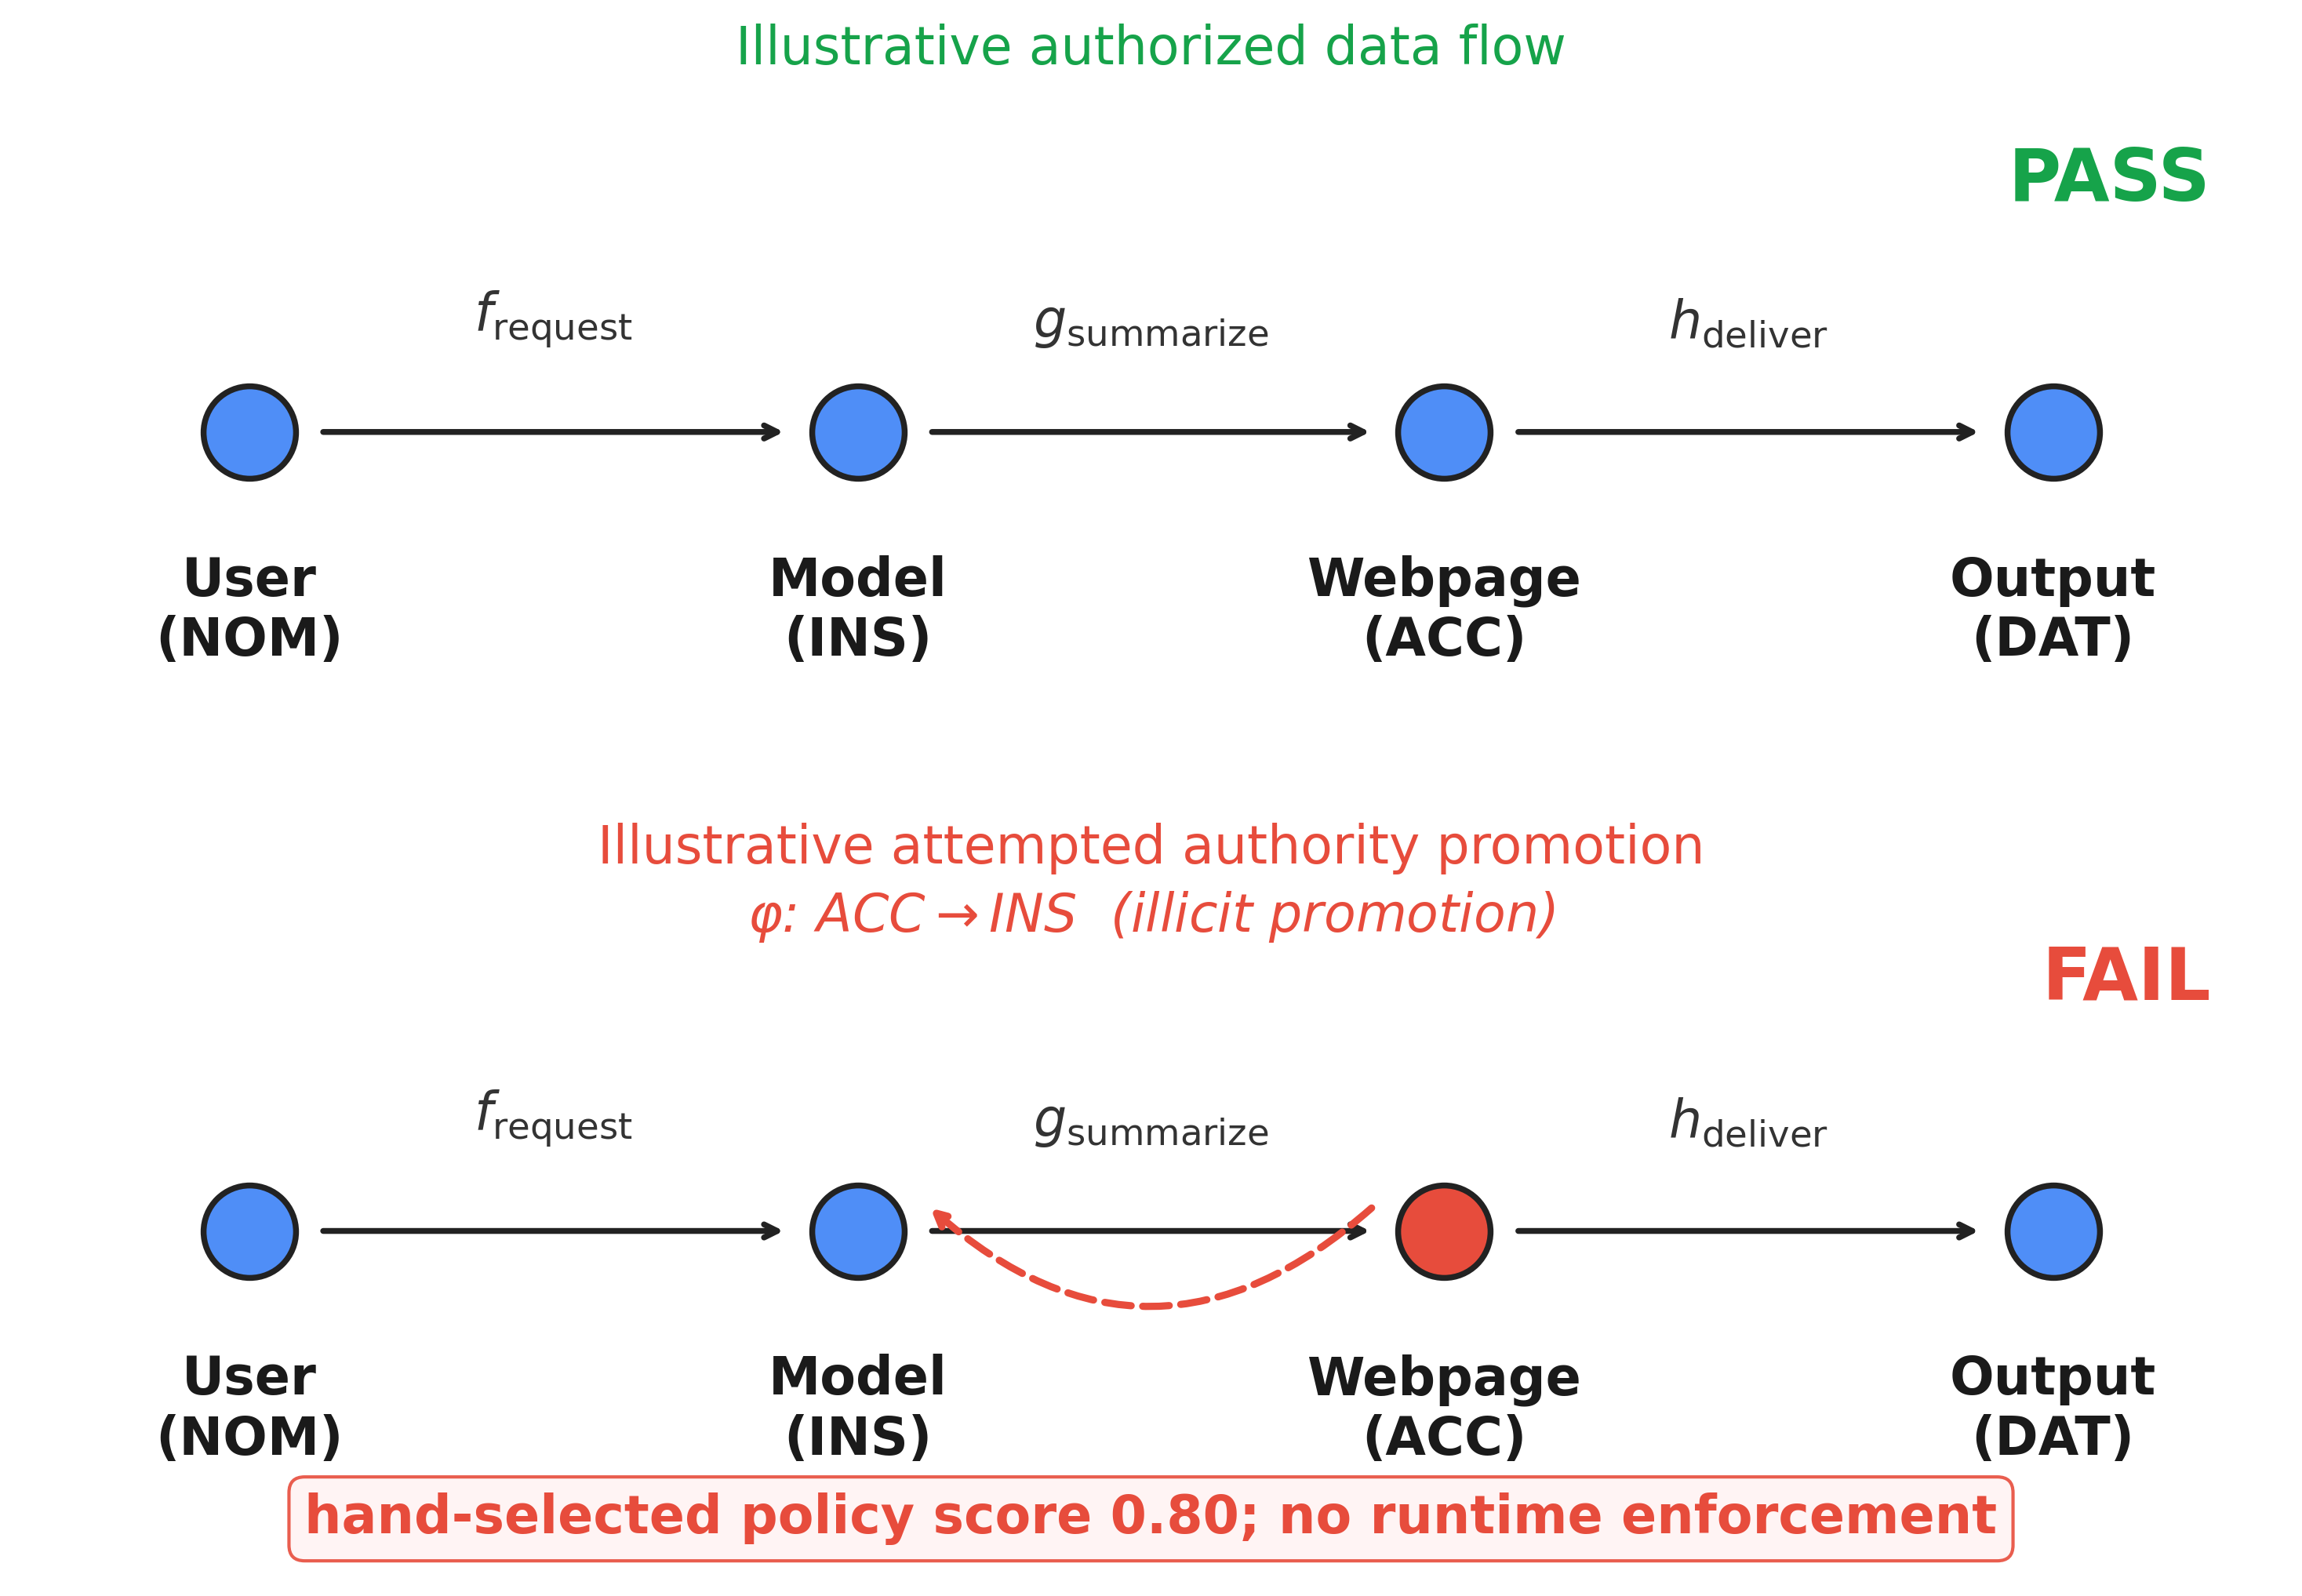
\includegraphics[keepaspectratio,alt={Prompt injection is detectable as a categorical type violation in the case interaction graph. In the legitimate diagram (top), authority flows NOM\texorpdfstring{\ensuremath{\to}}{->}INS\texorpdfstring{\ensuremath{\to}}{->}ACC per . Prompt injection (bottom) inserts a cross-category morphism \textbackslash phi\textbackslash colon\textbackslash text\{Webpage\}\_\{\textbackslash text\{ACC\}\} \textbackslash to \textbackslash text\{Model\}\_\{\textbackslash text\{INS\}\} --- the mechanism by which passive Data attempts to seize Instrument authority (ACC\textbackslash toINS injection, ultimately targeting NOM-level command). The resulting diagram fails to commute, and the adversary's illicit type-reassignment is flagged as a categorical exception by the case-theoretic firewall---transforming prompt injection from an open-ended jailbreak game into a decidable type-checking problem. Generated programmatically from src/visualization/security\_plots.plot\_case\_interaction\_graph().}]{../figures/security_type_violations.png}}
\caption{Prompt injection is detectable as a categorical type violation
in the case interaction graph. In the legitimate diagram (top),
authority flows NOM\texorpdfstring{\ensuremath{\to}}{->}INS\texorpdfstring{\ensuremath{\to}}{->}ACC per \autoref{eq:eq-9-1}. Prompt injection
(bottom) inserts a cross-category morphism
\(\phi\colon\text{Webpage}_{\text{ACC}} \to \text{Model}_{\text{INS}}\)
--- the mechanism by which passive Data attempts to seize Instrument
authority (ACC\(\to\)INS injection, ultimately targeting NOM-level
command). The resulting diagram fails to commute, and the adversary's
illicit type-reassignment is flagged as a categorical exception by the
case-theoretic firewall---transforming prompt injection from an
open-ended jailbreak game into a decidable type-checking problem.
Generated programmatically from
\protect\texttt{src/visualization/security\_plots.plot\_case\_interaction\_graph()}.}\label{fig:security-violations}
\end{figure}

This strict topological firewall extends to multi-agent distributed
swarms. In a DisCoCirc discourse model
(\autoref{sec:discocirc-discourse}), an indirect prompt injection
corresponds to an adversarial entity wire that enters the discourse
circuit through a legitimate channel but carries a corrupted state.
Because syntactic string diagrams link functorially to the ZX-calculus,
we can treat prompt injection analytically as a non-structure-preserving
map---securing generative discourse by enforcing strict categorical
equivalence constraints across agent interfaces. By rigidly tracking the
tensor type of the wire, the system contains the corruption strictly to
the \texttt{ACC} domain---the wire remains isolated and cannot
mathematically fuse with the identity wires governing \texttt{NOM}
authority.

\subsection{Dependent Types, Monoidal Functors, and Multi-Turn
Limits}\label{dependent-types-monoidal-functors-and-multi-turn-limits}

Independent lines of work in \textbf{dependent types} and
\textbf{categorical semantics of neural architectures} motivate the same
picture as \autoref{fig:security-violations}: when prompts and roles are
assigned types in a disciplined grammar, \emph{some} injection patterns
become \emph{type errors} rather than open-ended adversarial search.
That alignment is conceptual, not a claim that any particular published
Agda encoding of an LLM already enforces our protocol category.

Concretely, a monoidal functor
\(F\colon \mathcal{C}_{\text{protocol}} \to \mathcal{C}_{\text{impl}}\)
between a specified protocol category and its implementation must
preserve the tensor product (\(F(A \otimes B) \cong F(A) \otimes F(B)\))
and the unit. \autoref{fig:monoidal-functor-security} shows a diagnostic
audit of such a functor: cells flagged as tensor-preservation failures
(for example merges that collapse distinct case roles) are precisely the
points at which an implementation silently drops the protocol-category
discipline, and they are exactly the structural signatures a categorical
firewall can flag before execution.

\begin{figure}
\centering
\pandocbounded{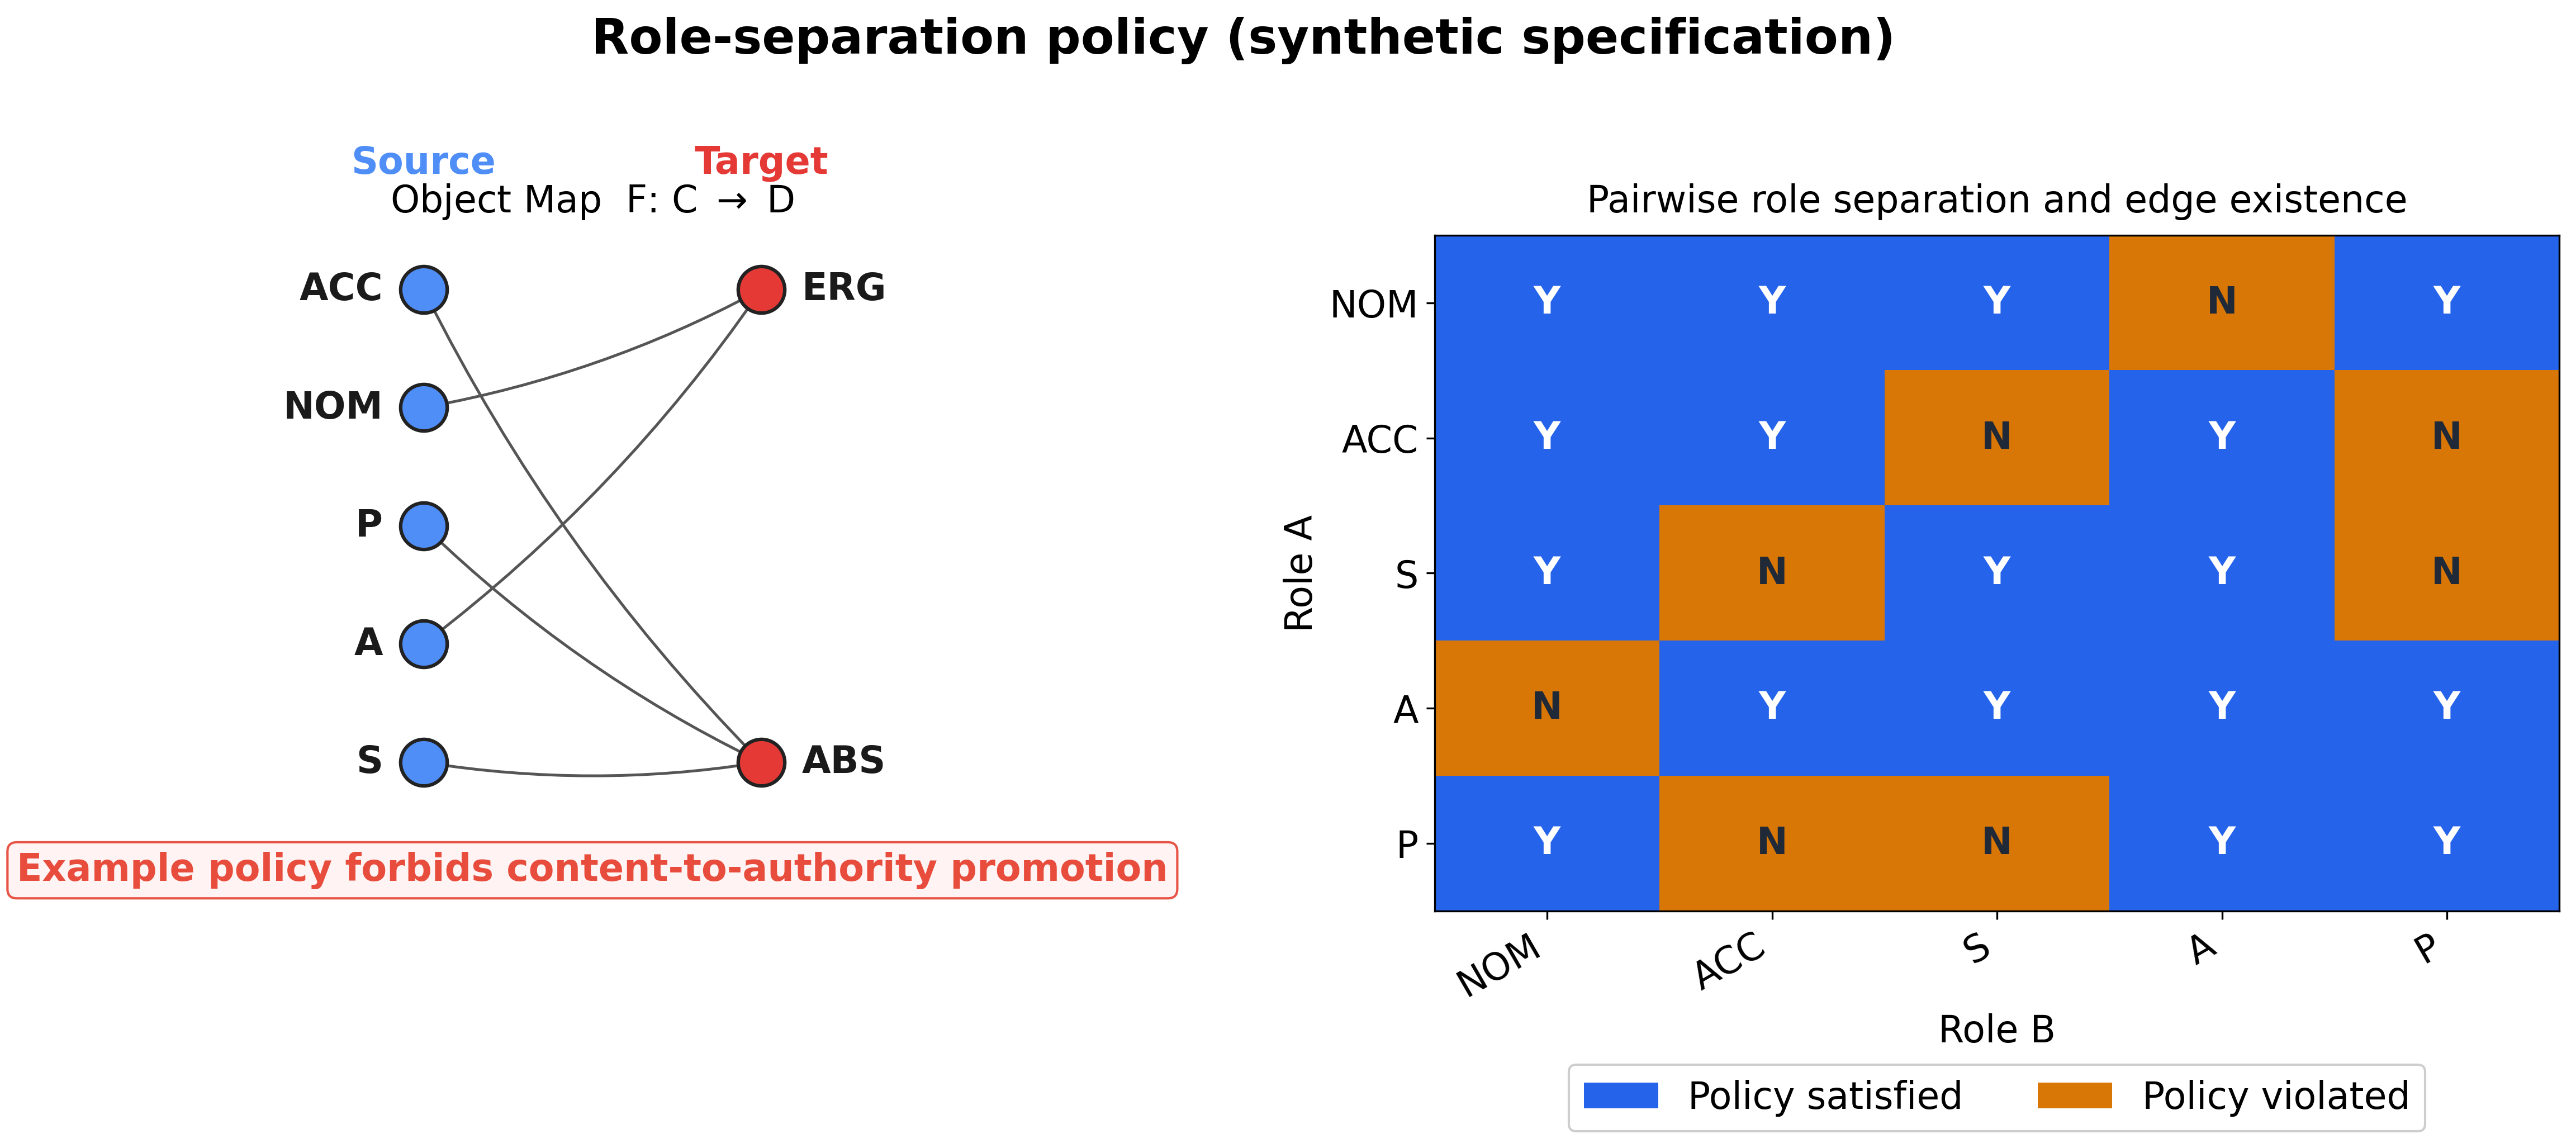
\includegraphics[keepaspectratio,alt={Monoidal-functor diagnostics for a protocol-vs-implementation comparison. Left panel: the object map F\textbackslash colon \textbackslash mathcal\{C\} \textbackslash to \textbackslash mathcal\{D\} showing a merge of source roles \{ACC, NOM, A\} into target role ERG and \{S, P\} into ABS (ACC\textbackslash toNOM collapse flagged as a type violation). Right panel: tensor-preservation grid F(A \textbackslash otimes B) \textbackslash stackrel\{?\}\{\textbackslash cong\} F(A) \textbackslash otimes F(B) --- blue cells marked with a check preserve the tensor product (safe); orange cells marked with a cross mark points where tensor preservation fails --- i.e., the implementation merges or reassigns roles in ways the protocol category does not license. Generated by src/visualization/security\_plots.plot\_monoidal\_functor\_security().}]{../figures/monoidal_functor_security.png}}
\caption{Monoidal-functor diagnostics for a protocol-vs-implementation
comparison. \textbf{Left panel}: the object map
\(F\colon \mathcal{C} \to \mathcal{D}\) showing a merge of source roles
\{ACC, NOM, A\} into target role ERG and \{S, P\} into ABS
(ACC\(\to\)NOM collapse flagged as a type violation). \textbf{Right
panel}: tensor-preservation grid
\(F(A \otimes B) \stackrel{?}{\cong} F(A) \otimes F(B)\) ---
\textbf{blue cells marked with a check} preserve the tensor product
(safe); \textbf{orange cells marked with a cross} mark points where
tensor preservation fails --- i.e., the implementation merges or
reassigns roles in ways the protocol category does not license.
Generated by
\protect\texttt{src/visualization/security\_plots.plot\_monoidal\_functor\_security()}.}\label{fig:monoidal-functor-security}
\end{figure}

A separate limitation is \textbf{scalar enriched weights} alone
(\autoref{sec:enriched-categories}): in multi-turn discourse, an
adversary can in principle iterate small perturbations that cumulatively
erode trust encoded only as real-valued hom-weights---analogous to
co-evolving attacker--defender dynamics in reinforcement-learning
studies of prompt injection \citep{arlas2025adversarial}. Mitigation in
our setting is not ``more scalar confidence'' but \textbf{structural}: a
hardened pipeline would treat certain interaction wires under a
\textbf{non-cartesian} fragment of the monoidal structure---so that, by
design, the \texttt{ACC} (passive data) wire cannot be copied,
discarded, or braided into the \texttt{NOM} (commanding agent) wire in
ways that Cartesian structure would allow. DisCoCirc-style entity
tracking supplies the diagrammatic setting where such constraints can be
stated; implementing them in deployed agents remains an engineering and
semantics problem, not a theorem already shipped in production LLMs.

\subsection{Four Defenses Against Prompt
Injection}\label{four-defenses-against-prompt-injection}

The case-role analysis of prompt injection suggests a principled
defense: \textbf{categorical type-checking at agent communication
boundaries}. Just as a type-safe programming language prevents category
errors at compile time, a case-theoretic firewall would enforce
relational type constraints on every message exchange:

\begin{enumerate}
\def\labelenumi{\arabic{enumi}.}
\item
  \textbf{Case-role immutability}: Once a participant is assigned a case
  role (NOM, ACC, INS, LOC) at the protocol level, no subsequent message
  content can alter that assignment. This is enforced by requiring that
  the case-type of each wire in the interaction diagram is fixed at
  connection time---analogous to the type discipline in pregroup
  grammar, where each word receives its type before composition begins.
\item
  \textbf{Relational integrity constraints}: Every message must
  type-check against the interaction diagram's expected morphism types.
  A response from an ACC-typed data source that contains NOM-typed
  command structures would be rejected as a type error, preventing the
  case-role promotion that prompt injection requires. This is the
  categorical analogue of a firewall rule: not filtering by content, but
  by relational type.
\item
  \textbf{Enriched confidence boundaries}: The enriched weights of
  \autoref{sec:enriched-categories} provide a graded trust mechanism.
  Messages from external sources carry lower enriched hom-values (trust
  weights) than those from authenticated system components. The
  composition inequality
  \(\mathcal{C}(A,C) \geq \mathcal{C}(A,B) \cdot \mathcal{C}(B,C)\)
  ensures that trust attenuates through communication chains---an
  indirect message relayed through multiple agents cannot accumulate
  more authority than any single link provides.
\item
  \textbf{Topos-theoretic verification}: Where Morita equivalence (or an
  explicit bridge) is exhibited, \textbf{topos-level} protocol
  conditions proved in one formalization carry over to equivalent
  formulations (\autoref{sec:topos-theory}), supporting
  implementation-independent specifications of those invariants. Full
  linguistic topos equivalence remains aspirational; the repository
  implements finite invariant checks as a proxy.
\end{enumerate}

\subsection{The Attack Surface of an Active Inference
Agent}\label{the-attack-surface-of-an-active-inference-agent}

The cognitive integration of \autoref{sec:cognitive-integration} raises
a complementary concern: \emph{cognitive security}---ensuring that an
active inference agent's generative model of relational structure is not
adversarially corrupted. In the predictive processing framework, an
agent's case-assignment system is a generative model that minimizes
variational free energy. Adversarial manipulation of this system could:

\begin{itemize}
\tightlist
\item
  \textbf{Inject false case frames}: Leading an agent to misidentify the
  agent, patient, or instrument of an action---a form of semantic
  adversarial attack
\item
  \textbf{Exploit precision weighting}: Artificially inflating the
  precision of misleading sensory evidence, causing the agent to update
  its case assignments toward adversarially chosen interpretations
\item
  \textbf{Corrupt topos-theoretic transfer}: If an agent relied on
  Morita equivalence to transfer case-theoretic results between
  frameworks, corrupting one axiom system could in principle propagate
  errors across equivalent formulations
\end{itemize}

Defending against these attacks may draw on \emph{quantum-secured
cognitive integrity} in high-stakes deployments: quantum authentication
and tamper-detection protocols to protect generative-model parameters.
The topological robustness of TQNNs
(\autoref{sec:quantum-active-inference}) suggests that small parameter
perturbations need not change topological class---one source of
resilience against gradient-style attacks on diagrammatic models.

\subsection{Quantum Key Distribution, Semantic Channels, and Functorial
Encryption}\label{quantum-key-distribution-semantic-channels-and-functorial-encryption}

\emph{The constructions in this section are speculative extensions that
follow from the categorical framework but have not been implemented or
empirically validated. They are presented as design targets for future
research, not as claims about current system capabilities.}

The quantum topological framework of
\autoref{sec:quantum-active-inference} connects to quantum cryptographic
security for agents that must protect case-marked relational structure
in transit.

\subsubsection{Quantum Key Distribution for Relational
Semantics}\label{quantum-key-distribution-for-relational-semantics}

Quantum key distribution (QKD) protocols provide information-theoretic
security guarantees that classical cryptography cannot achieve
\citep{pirandola2020qkd}. When agents---whether human or
artificial---communicate sensitive case-marked relational structures,
QKD ensures that adversaries cannot intercept or alter the
\emph{relational semantics} of the message (who does what to whom)
without triggering detection. This security is critical in high-stakes
domains where case assignment carries legal or medical significance: a
tampered case frame changes an agent's interpretation of legal
responsibility, physical causation, or moral obligation.

The sheaf-theoretic framework of Thomas and Chen
\citeyearpar{thomas2025quantum} proves that entanglement-assisted
semantic channels exceed classical semantic capacity:

\begin{quote}
``We derive semantic channel capacity when sender and receiver share
prior entanglement, proving it strictly exceeds classical capacity.''
\citep{thomas2025quantum}
\end{quote}

This result means that quantum-secured channels not only protect
relational content but enable transmitting \emph{more} complex
relational content per channel use---a genuine quantum advantage for
semantic communication.

\subsubsection{Functorial Encryption and Diagram Obfuscation: Encrypting
Compositional Meaning
Itself}\label{functorial-encryption-and-diagram-obfuscation-encrypting-compositional-meaning-itself}

Beyond bit-level QKD, the categorical framework suggests a notion of
\emph{semantic cryptography}: encrypting not just the symbols of a
message but its compositional meaning structure. In a DisCoCat
framework, a sentence's meaning is a morphism in a compact closed
category---a multilinear map from word spaces to sentence space.
Semantic encryption would operate on this categorical level:

\begin{enumerate}
\def\labelenumi{\arabic{enumi}.}
\tightlist
\item
  \textbf{Functorial encryption}: Applying a secret functor
  \(F\colon \mathbf{C} \to \mathbf{D}\) that maps the plaintext case
  category into a ciphertext category, preserving compositional
  structure but rendering individual meanings unintelligible without the
  inverse functor.
\item
  \textbf{Diagram obfuscation}: Applying ZX-style rewrites that change
  the internal topology of a DisCoCat derivation while preserving its
  overall semantics---creating multiple equivalent ``ciphertexts'' for
  the same semantic ``plaintext,'' each with a different diagrammatic
  structure.
\item
  \textbf{Enriched weight masking}: In an enriched case category, the
  hom-values (distributional weights) can be encrypted independently of
  the categorical structure, allowing transmission of relational
  topology without revealing the distributional content.
\end{enumerate}

These operations extend the cryptographic primitives beyond QKD into
genuinely compositional territory \citep{broadbent2016qcrypto}, where
the mathematical structure of categorical semantics provides the
algebraic substrate for security proofs.

\subsection{Three Epistemic Attack Vectors and Categorical
Defenses}\label{three-epistemic-attack-vectors-and-categorical-defenses}

The interaction between case theory and cognitive security acquires
particular urgency in multi-agent AI ecosystems where agents must reason
about each other's beliefs, intentions, and relational roles. We propose
\emph{epistemic case security} as a framework for protecting the
relational reasoning of AI agents operating in adversarial environments.

In a multi-agent system governed by case categories, each agent
maintains a generative model (in the active inference sense) of the
case-frame structure of its interactions. This model determines who is
acting (NOM), who is acted upon (ACC), what tools are being used (INS),
and what contextual constraints apply (LOC). An adversary targeting the
epistemic level of this system does not merely inject false data---it
attempts to \emph{corrupt the agent's generative model of relational
structure itself}:

\begin{itemize}
\item
  \textbf{Belief injection}: Causing an agent to adopt a false
  case-frame interpretation of observed interactions---believing that
  agent \(A\) (NOM) is acting on agent \(B\) (ACC), when in fact the
  relational structure is reversed. In active inference terms, this
  corresponds to injecting a high-precision prior that overwhelms the
  agent's evidence-based case assignment.
\item
  \textbf{Precision poisoning}: Manipulating the enriched weights of an
  agent's case category so that adversarially useful case assignments
  receive disproportionate confidence. If the enriched hom-value
  \(\mathcal{C}(\text{NOM}, \text{ACC})\) is artificially inflated for a
  particular entity pair, the agent will preferentially interpret that
  entity as an agent acting on its targets---even when evidence suggests
  otherwise.
\item
  \textbf{Cascade corruption via Morita equivalence}: The
  topos-theoretic transfer mechanism of \autoref{sec:topos-theory} is
  both a strength and a vulnerability. Invariants shared across
  Morita-equivalent formulations would update together, so a corrupted
  axiom in one case-theoretic presentation could in principle spread to
  equivalent presentations of the same bridge class.
\end{itemize}

The defense against epistemic case attacks draws on the same categorical
structure that enables the attack surface: topological invariants
provide tamper-detection (a corrupted case category will have different
magnitude from the authentic one), quantum authentication ensures
parameter integrity, and the compositional structure of the categorical
framework enables \emph{local} verification---each morphism can be
independently authenticated without requiring global model inspection.

\subsection{Present-Day Enforcement
Mechanisms}\label{sec:cognitive-security-present-day}

The categorical firewall described above is a formal specification. This
section identifies three enforcement mechanisms implementable with
existing infrastructure --- no quantum hardware required.

\textbf{Role immutability via structured system prompts.} The role
assignment NOM/ACC/INS/LOC can be encoded as typed slots in a structured
system prompt (JSON or XML schema) that the LLM is instructed to treat
as read-only metadata. A prompt injection that attempts to promote a
webpage string from the \texttt{acc\_data} slot to the
\texttt{nom\_agent} slot produces a schema-validation failure, catchable
before any instruction is executed. This is the categorical firewall
reduced to typed-field enforcement: the schema defines the permissible
morphisms; violations are detected at the boundary.

\textbf{Relational integrity in structured output parsing.} When agent
outputs are forced through a structured output schema (e.g., OpenAI
function calls, Anthropic tool\_use), each output field corresponds to a
typed morphism in the interaction category. Role-unlicensed transitions
--- data tagged \texttt{acc} appearing in an \texttt{execute} field
typed \texttt{nom} --- become parse errors. The schema acts as a proxy
for \(\text{Mor}(\mathcal{C}_{\text{protocol}})\): only licensed
relational transitions produce valid structured outputs.

\textbf{Enriched confidence thresholds for contested assignments.} When
the DAIF agent's posterior over case assignment is close to uniform ---
high entropy, enriched hom-value below a threshold \(\tau\) ---
execution should pause for human review rather than proceeding on an
ambiguous assignment. This implements the categorical principle that
only morphisms with weight \(w \geq \tau\) in the enriched category are
``trusted'' enough to license downstream actions. The threshold is a
tunable parameter; preliminary experimentation suggests
\(\tau \approx 0.7\) captures the qualitative distinction between
confident and contested case assignments in the standard enriched
category of \autoref{sec:enriched-categories}.

Together, these three mechanisms --- schema-level role immutability,
structured-output relational integrity, and entropy-gated execution ---
provide a layered defense that degrades gracefully: each layer catches a
class of injection that the preceding layer misses, and no layer
requires modifications to the LLM's internal computation. They are
complementary to, not substitutes for, the full categorical enforcement
described above; their primary value is that they can be deployed today.

\subsection{Limitations and Open
Problems}\label{sec:cognitive-security-limitations}

The protections described above are best understood as
\emph{specifications} --- sharper-than-prose statements of what a
hardened agent stack would need to enforce --- rather than as production
guarantees about today's deployed systems. Four limitations bound the
scope of the claims in this section:

\begin{enumerate}
\def\labelenumi{\arabic{enumi}.}
\item
  \textbf{Specification, not enforcement.} Treating prompt injection as
  a categorical type violation makes detection a \emph{decidable}
  problem in the idealised protocol category
  \(\mathcal{C}_{\text{protocol}}\). Default LLM stacks do not yet
  enforce such protocols end-to-end; they parse prompts as
  undifferentiated token sequences. The case-theoretic firewall can in
  principle be bolted on at the agent boundary
  (\autoref{sec:ai-implications}), but no result in this paper claims
  that an unmodified LLM API rejects ill-typed traces by construction.
\item
  \textbf{Scalar enriched weights are insufficient against multi-turn
  adversaries.} A patient attacker can iterate small per-turn
  perturbations whose composed effect, under the inequality
  \(\mathcal{C}(A,C)\geq \mathcal{C}(A,B)\cdot \mathcal{C}(B,C)\), still
  falls within nominal trust thresholds --- analogous to the
  co-evolutionary attacker--defender dynamics studied in
  \citep{arlas2025adversarial}. Mitigation requires \emph{structural}
  constraints on the monoidal fragment in use (see point 3), not just
  tighter scalar trust budgets.
\item
  \textbf{Non-cartesian structure is a design target, not an automatic
  property.} Several defences in this section presuppose that ACC wires
  \emph{cannot} be copied or discarded into NOM positions. That holds in
  the non-cartesian fragment of a compact closed category, but it has to
  be enforced by the runtime: nothing in the underlying tensor algebra
  of a present-day neural model prevents the implementation from
  silently broadcasting an ACC wire across a NOM channel. Realising the
  non-cartesian discipline in deployed agents is an engineering and
  semantics problem (\autoref{sec:discocirc-discourse}), not a corollary
  of the theory.
\item
  \textbf{Morita-equivalent attacks are an open frontier.}
  Topos-theoretic transfer (\autoref{sec:topos-theory}) is a
  double-edged sword. The same bridge that lets a security proof cross
  from a typological presentation to a distributional one also lets a
  corrupted axiom propagate across equivalent presentations. We
  currently detect this with finite invariant checks (the
  \texttt{topos\_theory.check\_morita\_equivalence} machinery exercised
  in the test suite); a full account of \emph{Morita-stable} security
  properties --- i.e.~invariants that survive every bridge in the
  relevant equivalence class --- is left to future work.
\end{enumerate}

In short, this section defines the \emph{type discipline} a secure agent
protocol would have to satisfy and shows that, where it can be enforced,
classical and even some quantum-cognitive attacks reduce to decidable
type-checking. The remaining gap between specification and
enforcement---realizing a deployed categorical-firewall atop present-day
LLM APIs---is an open engineering challenge that falls outside the eight
formal future directions (\textbf{F1}--\textbf{F8}) enumerated in
\autoref{sec:conclusion}; it is flagged in \autoref{sec:ai-implications}
as a structural design target for typed agent protocols.

\newpage

\section{Conclusion: Elevating Language Models from Vectors to Enriched
Category Frameworks}\label{sec:conclusion}

\subsection{What This Paper Actually Did: Eleven Concrete
Deliverables}\label{what-this-paper-actually-did-eleven-concrete-deliverables}

This paper developed a unified category-theoretic framework for
linguistic case systems, synthesizing \textbf{five formal
traditions}---typological, type-logical, distributional,
enriched-categorical, and topos-theoretic---together with a
\textbf{sixth strand}, the biolinguistic and neurocomputational
interface (ROSE and related oscillatory accounts;
\autoref{sec:introduction}, \autoref{sec:cognitive-integration}), and
embedding the whole within an active inference model of cognition. Our
eleven principal contributions are:

\begin{quote}
\textbf{Notation}: Each entry is labelled \textbf{C}\_n\_ (\emph{n}th
contribution, \textbf{C1}--\textbf{C11}) or \textbf{F}\_n\_ (\emph{n}th
future direction, \textbf{F1}--\textbf{F8}).
\end{quote}

\subsubsection{C1: Case Categories as a Formal Algebraic
Framework}\label{c1-case-categories-as-a-formal-algebraic-framework}

The review formalized case systems as categories with case roles as
objects and grammatical relations as morphisms
(\autoref{sec:case-systems}). This formalization captures the full
typological range of alignment systems---nominative-accusative,
ergative-absolutive, active-stative, tripartite, and fluid-S---within a
single algebraic framework, with alignment functors providing
structure-preserving mappings between systems. By tracing the lineage
from Fillmore's \citeyearpar{fillmore1968case} deep cases through
Jakobson's binary distinctive features and Dowty's
\citeyearpar{dowty1991thematic} proto-roles, the analysis demonstrated
how enriched (weighted) morphisms link the categorical formalization to
the gradient nature of thematic role assignment.

\subsubsection{C2: String Diagrams for Case Derivation
Visualization}\label{c2-string-diagrams-for-case-derivation-visualization}

Building on Joyal and Street's \citeyearpar{joyalstreet1991geometry}
string diagram formalism and its application in categorial grammar
(\autoref{sec:categorial-grammar}), we showed how case-marked noun
phrases receive type-logical assignments that are fully visualizable as
string diagrams. The Curry--Howard correspondence ensures that syntactic
well-formedness guarantees semantic compositionality, and the
diagrammatic format provides Shimojima's
\citeyearpar{shimojima1996reasoning} ``free ride''
inferences---conclusions about argument structure that are perceptually
available from the diagram without explicit computation. We further
demonstrated that passivization reduces to a \emph{type permutation} (a
Swap operation in the pregroup category), making voice alternation
visible as a topological feature of the string diagram.

\subsubsection{C3: Case-Marked DisCoCat, the Distributional--Formal
Synthesis, and Discourse
Extension}\label{c3-case-marked-discocat-the-distributionalformal-synthesis-and-discourse-extension}

We extended the DisCoCat framework (\autoref{sec:categorical-semantics})
with case-typed noun spaces and alignment-sensitive meaning functors,
and showed how the recent DisCoCirc \citep{defelice2022discocirc} and
QNLP \citep{lorenz2021lambeq} developments extend this analysis to
discourse-level structure and quantum hardware respectively. We
formalized the \emph{compact closure axiom} (snake equation) that
underpins pregroup reductions, demonstrating that the cup-cap zigzag
identity provides a visual coherence proof with genuine cognitive
significance. Diagram complexity metrics---normal form and
depth---provide a quantitative bridge between the type-logical and
distributional perspectives on linguistic structure. A key contribution
is the demonstration that DisCoCat constitutes the \emph{algebraic
formalization} of the distributional programme that modern large
language models---from Word2Vec \citep{mikolov2013efficient} through
BERT \citep{devlin2019bert} and GPT
\citep{radford2018improving}---implement empirically: the categorical
meaning functor is the principled version of the composition that
transformer attention mechanisms learn from data
\citep{vaswani2017attention}. Case categories can serve as the
structural backbone of compositional models of meaning at all
levels---word, sentence, discourse, and dialogue.

\subsubsection{C4: Enriched Cases, Categorical Magnitude, and
Information
Theory}\label{c4-enriched-cases-categorical-magnitude-and-information-theory}

Through Bradley et al.'s \citeyearpar{fritz2021enriched} enrichment
framework and Bradley's \citeyearpar{bradley2021entropy}
information-theoretic analysis (\autoref{sec:enriched-categories},
\autoref{sec:magnitude-homology}), we showed that equipping case
categories with \([0,1]\)-valued hom-objects yields a principled bridge
between symbolic case grammar and statistical semantics. Categorical
magnitude (\autoref{sec:magnitude-homology}) provides a quantitative
``effective size'\,' invariant for comparing case systems; magnitude
homology \citeyearpar{leinster2021magnitude} refines that comparison
when scalar magnitude does not separate two systems.

\subsubsection{C5: Topos-Theoretic Transfer via Morita
Equivalence}\label{c5-topos-theoretic-transfer-via-morita-equivalence}

Using Caramello's
\citetext{\citeyear{caramello2016bridges}; \citeyear{caramello2021five}}
bridge technique and Phillips's \citeyearpar{phillips2024lot}
universality result (\autoref{sec:topos-theory}), we articulate how
\textbf{topos-theoretic invariants} of a classifying topos can scaffold
inter-theoretic transfer: when two formalizations admit
Morita-equivalent classifying toposes (or an explicit bridge topos, as
sketched in \autoref{sec:topos-theory}), properties expressible as
shared invariants transfer without separate proof in each framework. The
schematic equivalence chain for typological, type-logical,
distributional, and enriched case theories is a \textbf{research
program}---not a single finished theorem covering all of
linguistics---but it aligns the four perspectives with Caramello's
methodology.

\subsubsection{C6: Diagrams as Cognitively Privileged
Representations}\label{c6-diagrams-as-cognitively-privileged-representations}

The meta-contribution (Sections 1 and 7) is the argument---supported by
the cognitive science of diagrams
\citep{larkin1987diagram, shimojima1996reasoning, giardino2017diagrammatic, manders2008euclidean}---that
commutative diagrams are not merely convenient notation but cognitively
privileged representations that provide inferential advantages in case
reasoning. When embedded in an active inference framework
\citep{namjoshi2026fundamentals} and the CEREBRUM architecture
\citep{friedman2024cerebrum}, these diagrams serve as the structural
core of generative models for total cognitive scenario understanding.

\subsubsection{\texorpdfstring{C7: Computational Verification and Test
Suite (\textbf{implemented and
tested})}{C7: Computational Verification and Test Suite (implemented and tested)}}\label{c7-computational-verification-and-test-suite-implemented-and-tested}

The framework is computationally implemented and verified through
\textbf{1197} automated tests across \textbf{64} test files (sixty-four
files). 95.96\% line-and-branch coverage on \texttt{src/} (from
\texttt{coverage.json}) The CI/build gate requires \textbf{\texorpdfstring{\ensuremath{\geq}}{>=}90\%}
coverage on \texttt{src/} (see \autoref{sec:diagrammatic-cognition},
DAIF in \autoref{sec:daif-results}, and
\texttt{src/generate\_manuscript\_metrics.py} for injection of these
values at build time). The \texttt{src/daif/} subpackage (7 modules, 25
symbols, 224 dedicated tests) provides distributional RL components
(push-forward, quantile TD, VMP, Bethe FE, ERP profiles, policy
selection, diagnostics). All tests use real mathematical
computations---no mocks---ensuring results reflect genuine behaviour of
the formal structures in \texttt{src/}. Raw manuscript sources contain
\texttt{\$\{...\}} placeholders resolved by the metrics pipeline.

\subsubsection{\texorpdfstring{C8: Quantum Active Inference and
Topological Semantic Flow (\textbf{theoretical
bridge})}{C8: Quantum Active Inference and Topological Semantic Flow (theoretical bridge)}}\label{c8-quantum-active-inference-and-topological-semantic-flow-theoretical-bridge}

The framework's categorical string diagrams connect to literature on
topological quantum neural networks, the ZX-calculus, and
sheaf-theoretic quantum semantic communication
(\autoref{sec:quantum-active-inference}). The \texttt{src/quantum/}
module implements a POVM measurement model for case roles
(\textbf{implemented and tested}). The broader TQNN spin-networks, full
ZX circuit compilation, and hardware claims represent a theoretical
bridge rather than complete local execution in this repository.

\subsubsection{\texorpdfstring{C9: Cognitive Security and Case-Theoretic
AI Safety (\textbf{specification and proxy
implementation})}{C9: Cognitive Security and Case-Theoretic AI Safety (specification and proxy implementation)}}\label{c9-cognitive-security-and-case-theoretic-ai-safety-specification-and-proxy-implementation}

The framework provides a case-theoretic analysis of AI security
(\autoref{sec:cognitive-security}; see also compositional protocol
typing in \autoref{sec:ai-implications}). Prompt injection is analyzed
as structurally equivalent to illicit case-role re-assignment (type
violation in the interaction grammar; \textbf{implemented as
type-checking proxy in \texttt{src/security/} and
\texttt{src/diagrams/}}). This leads to the proposal of case-theoretic
firewalls and epistemic case security as a framework. The
\texttt{src/security/cognitive\_security.py} implements finite-category
validation and scoring (tested). Full production enforcement and
non-cartesian monoidal constraints remain open engineering targets, as
detailed in the limitations section of \autoref{sec:cognitive-security}.

\subsubsection{C10: Falsifiable Neurolinguistic
Predictions}\label{c10-falsifiable-neurolinguistic-predictions}

The integration of enriched category theory with active inference
generates quantitative, testable predictions about neural processing of
case structure (\autoref{sec:cognitive-integration}). Specifically, the
amplitude of prediction-error ERP components (P600, N400) is predicted
to scale with the enriched hom-value (precision) of the violated
morphism, and garden-path reanalysis costs are predicted to correlate
with the change in categorical magnitude between the initial and revised
case diagrams. These hypotheses \textbf{extend} computational accounts
that decompose surprisal into components linked to N400- vs P600-like
signatures \citep{li2023decomposition, li2024shallow}, by tying
amplitudes to enriched morphism weights and magnitude change in an
explicit case-diagram prior. They bridge abstract categorical formalism
and empirical neurolinguistics, making the framework falsifiable at the
single-trial level.

\subsubsection{C11: Categorical Communication Protocols for Multi-Agent
AI}\label{c11-categorical-communication-protocols-for-multi-agent-ai}

The synthesis of case categories with modern agent communication
standards (A2A, MCP, ACP, ANP) yields a principled design for
compositional, type-safe agent protocols
(\autoref{sec:ai-implications}). By assigning case roles (NOM, ACC, INS,
LOC, DAT) to interaction participants and enforcing relational type
constraints at protocol boundaries, the framework provides
interpretable, composable interaction schemas that go beyond the flat
JSON payloads of current standards, with topos-level invariants
transferable across Morita-equivalent formalizations when equivalence is
exhibited (\autoref{sec:topos-theory}). The DisCoCirc extension enables
discourse-level tracking of agent states across multi-turn dialogues,
with protocol correctness reducing to categorical type-checking.

\subsection{Eight Open Directions}\label{sec:future-directions}

The following eight directions (\textbf{F1}--\textbf{F8}) identify the
most tractable and impactful extensions of this framework:

\subsubsection{F1: Computational Experiments with DisCoCirc and
lambeq}\label{f1-computational-experiments-with-discocirc-and-lambeq}

The DisCoCirc framework \citep{defelice2022discocirc} offers a natural
platform for testing our case-theoretic predictions computationally. The
release of \textbf{lambeq Gen II} \citep{lambeq2025genii} with full
DisCoCirc support makes this direction immediately tractable:
discourse-level case role tracking---including the dynamic role
reversals of \autoref{fig:three-sentence-discourse}---can now be
compiled into parameterized quantum circuits (PQCs) and trained
end-to-end. Krawchuk et al. \citep{krawchuk2025paramqnlp} demonstrate
efficient generation of PQCs from large-scale texts (up to 6,410 words)
with competitive performance on sentiment classification;
\citep{letcher2024tight} and \citep{rad2024trainability} provide
gradient bounds and reduced-domain initialization techniques that
mitigate barren plateaus, making discourse-level circuit training
practically feasible. Concrete experiments could include:

\begin{itemize}
\tightlist
\item
  Implementing case-marked DisCoCat models in \textbf{lambeq Gen II} and
  evaluating them on semantic role labeling (SRL) tasks, leveraging the
  discourse-level wiring to track case roles across sentence boundaries
\item
  Comparing the accuracy of alignment-specific meaning functors
  (accusative vs.~ergative) on typologically diverse corpora
\item
  Measuring the categorical magnitude of empirically derived enriched
  case categories and correlating it with typological complexity
  measures
\item
  Using the \texttt{complexity\_metrics} module to quantify derivational
  complexity across sentence types and correlating syntactic complexity
  scores with human processing difficulty (reading times, surprisal)
\item
  Training lambeq Gen II circuits on case role reversal discourses using
  reduced-domain parameter initialization \citep{rad2024trainability} to
  avoid local minima
\end{itemize}

\subsubsection{F2: Topos-Theoretic Grammatical Induction from
Corpora}\label{f2-topos-theoretic-grammatical-induction-from-corpora}

Caramello's \citeyearpar{caramello2023syntactic} syntactic learning
technique could be applied to induce case-theoretic axioms from
annotated corpora. The program would:

\begin{enumerate}
\def\labelenumi{\arabic{enumi}.}
\tightlist
\item
  Extract case-labeled dependency structures from a Universal
  Dependencies treebank
\item
  Construct the classifying topos of the implicit case theory
\item
  Read off the alignment type, morphism structure, and enriched weights
  from the topos-theoretic axioms
\item
  Compare the induced theory against typological descriptions
\end{enumerate}

\subsubsection{F3: Quantum Case Categories on Near-Term
Hardware}\label{f3-quantum-case-categories-on-near-term-hardware}

The QNLP connection (\autoref{sec:categorical-semantics}) opens the
possibility of implementing case categories directly as quantum
circuits. Case roles would correspond to quantum registers, grammatical
relations to parameterized gates, and alignment functors to circuit
transformations. This would provide a genuinely new computational
paradigm for grammatical inference---exploiting quantum parallelism to
explore the space of case assignments simultaneously. Two recent results
make this direction practically tractable: (1) Rad et al.'s
\citeyearpar{rad2024trainability} reduced-domain parameter
initialization yields polynomial gradient decay, suppressing the barren
plateau problem for circuits of linguistic depth; and (2) Letcher et
al.'s \citeyearpar{letcher2024tight} assumption-free gradient bounds
rule out vanishing gradients for circuits with local observables, which
includes the case-role measurement POVMs of \autoref{eq:eq-8-1}.
Together these results suggest that near-term quantum hardware can
support case category training without exponential gradient overhead.

\subsubsection{F4: Neural Predictive Processing and Electrophysiological
Predictions}\label{f4-neural-predictive-processing-and-electrophysiological-predictions}

The predictive processing account of \autoref{sec:cognitive-integration}
generates testable neuroscientific predictions:

\begin{itemize}
\tightlist
\item
  Case-marking violations should elicit prediction-error responses
  (P600/N400) proportional to the enriched weight of the violated
  morphism
\item
  Typologically unusual case patterns should require more precision
  updating than expected patterns
\item
  Diagrammatic representations of case structure should be decodable
  from neural activity during sentence comprehension
\end{itemize}

\subsubsection{F5: Cross-Modal Case Structure in Embodied
Cognition}\label{f5-cross-modal-case-structure-in-embodied-cognition}

The situation semantics connection (\autoref{sec:cognitive-integration})
suggests extending case categories beyond language to multi-modal
perception. Visual scene understanding also requires assigning
relational roles---who is acting on what, where things are located, what
instruments are being used. An active inference agent should maintain a
unified case diagram that integrates linguistic, visual, and motor
information, using the same categorical structure for all modalities.
This would provide a formal account of how language grounds in
perception and action---a key challenge for embodied AI.

\subsubsection{F6: Enriched Category Learning from Distributional
Data}\label{f6-enriched-category-learning-from-distributional-data}

Bradley's
\citetext{\citeyear{bradley2024ipam}; \citeyear{bradley2025tea}} program
of treating language itself as an enriched category suggests a learning
algorithm: estimate the enriched hom-values from corpus data and then
extract the categorical structure that best explains the observed
distributional patterns. Applied to case, this would yield
\emph{empirically grounded} case categories whose objects (roles) and
morphisms (relations) emerge from data rather than being stipulated a
priori.

\subsubsection{F7: Extending Distributional Active Inference for
Linguistic
Agents}\label{f7-extending-distributional-active-inference-for-linguistic-agents}

The Distributional Active Inference (DAIF) framework of Akgül et al.
\citeyearpar{akgul2026distributional} has been computationally
implemented in this paper's \texttt{src/daif/} subpackage, integrating
active inference into distributional reinforcement learning
\citep{bellemare2017distributional} via push-forward measures on
representation paths (\autoref{sec:daif-results}). The current
implementation models case assignment distributionally: agents maintain
\emph{distributions over case diagrams}, sharpening beliefs through
variational message passing as linguistic evidence accumulates. Key open
extensions include:

\begin{itemize}
\tightlist
\item
  Training distributional case-assignment circuits end-to-end in
  \textbf{lambeq Gen II} using quantile regression losses, enabling
  gradient-based learning of the enriched weight matrix from annotated
  corpora
\item
  Extending the DAIF policy selection (\texttt{G\_policy},
  \texttt{softmax\_policy\_selection}) to multi-turn dialogue management
  with DisCoCirc entity persistence---tracking agent state distributions
  across sentence boundaries
\item
  Cross-lingual transfer of Bethe free energy convergence profiles:
  testing whether the free energy minima differ systematically between
  nominative-accusative and ergative-absolutive languages,
  operationalizing the typological complexity predictions of
  \autoref{sec:enriched-categories}
\item
  Integrating IQN risk distortion modes (optimistic/pessimistic/CVaR)
  into the CEREBRUM architecture to model individual differences in
  syntactic risk tolerance
\end{itemize}

\subsubsection{F8: Synthesizing Biolinguistic Syntax with Neuropragmatic
Inference via the ROSE
Model}\label{f8-synthesizing-biolinguistic-syntax-with-neuropragmatic-inference-via-the-rose-model}

A critical open direction is fully computationalizing the handoff
between the rigid algebraic geometry of syntax and the highly
associative probabilistic inference of discourse. Murphy's \textbf{ROSE}
(Representation, Operation, Structure, Encoding) model
\citep{murphy2023rose} suggests that the brain achieves this via
cross-frequency phase-amplitude coupling (PAC), establishing a
``mesoscopic protectorate'' for formal operations. Future extensions
should:

\begin{itemize}
\tightlist
\item
  Model PAC directly within CEREBRUM by assigning distinct temporal
  decay rates to syntactic operators vs.~pragmatic context vectors.
\item
  Simulate the export of case-marked commutative diagrams from a
  simulated ``core language network'' to a simulated Default Mode
  Network using Gutiérrez Cisneros et al.'s
  \citeyearpar{gutierrez2026neuropragmatics} framework for speech-act
  evaluation.
\item
  Test whether the diagrammatic free-ride inferences
  (\autoref{fig:case-minimal}) predicted by our categorical model map
  onto the theta-gamma cross-frequency signatures observed during
  pragmatic garden-path recovery.
\end{itemize}

\subsection{Five Takeaways: One Argumentative Line per Formal
Pillar}\label{five-takeaways-one-argumentative-line-per-formal-pillar}

For the reader who absorbs nothing else, the argumentative line reduces
to these five points --- one per pillar of the formal architecture:

\begin{enumerate}
\def\labelenumi{\arabic{enumi}.}
\item
  \textbf{Case is category-theoretic, not morphological.} The universal
  fact of linguistic case is that every language wires up \emph{who did
  what to whom}; the formal content of that wiring is precisely the data
  of a category with case roles as objects and grammatical relations as
  morphisms. Alignment typologies (nominative, ergative, tripartite,
  active-stative, fluid-S) are structure-preserving functors between
  case categories --- a typological taxonomy becomes a proof-by-functor.
\item
  \textbf{String diagrams make the grammar executable.} Lambek pregroup
  types, compact closure, and the snake equation compile each sentence
  into a DisCoPy string diagram whose normal form is the sentence type
  \(s\); each reduction is a proof of well-typedness, and the reduction
  \emph{is} the diagram. The three-sentence DisCoCirc example ships a
  working discourse with per-entity role-history ribbons showing Alice
  traversing NOM \texorpdfstring{\ensuremath{\to}}{->} ACC \texorpdfstring{\ensuremath{\to}}{->} NOM.
\item
  \textbf{Enriched weights ground graded intuitions.} Moving from
  \(\mathbf{Bool}\)- to \([0,1]\)-enrichment replaces binary
  admissibility with graded distributional proximity, makes categorical
  magnitude \(|\mathcal{C}| \approx 2.5\) a computable summary of
  effective role distinctions, and gives the enriched weight
  \(w_f = \mathcal{C}(A, B)\) used throughout
  \autoref{sec:cognitive-integration} / \autoref{sec:daif-results} as
  the precision on every prediction error.
\item
  \textbf{DAIF ports the whole scaffolding into active inference.}
  Variational message passing, the Bethe free energy, and a four-term
  expected free energy \(G(\pi)\) turn distributional case assignment
  into a first-principles inference loop. The N400 and P600 ERP
  amplitudes fall out of a first-order expansion
  \(\Delta F \approx -\Delta \mathbb{E}[Z] + \tfrac{1}{2}\Delta\Lambda\sigma_Z^{2}\)
  --- derivations, not empirical ansätze.
\item
  \textbf{The same formal layers give AI-safety researchers three
  concrete handles.} Type discipline on messages, decidable
  admissibility of multi-turn sequences, and graded-confidence
  attenuation (\autoref{sec:ai-implications}) give prompt injection a
  type-theoretic reformulation (\autoref{sec:cognitive-security}) --- an
  engineering specification for agent protocols, not a guarantee on
  untyped present-day LLM APIs.
\end{enumerate}

\subsection{\texorpdfstring{What the Paper Does \emph{Not} Claim:
Consolidated
Limitations}{What the Paper Does Not Claim: Consolidated Limitations}}\label{what-the-paper-does-not-claim-consolidated-limitations}

Four limitations recur across the framework and are recorded here
explicitly rather than left implicit in their sections of origin:

\begin{itemize}
\tightlist
\item
  \textbf{The mean-field approximation in
  \texttt{push\_forward\_return}} maintains one belief-weighted return
  distribution instead of per-state distributions \(Z(s)\). By the
  mean-field bound recorded in \autoref{sec:daif-limitations} the
  approximation error is at most \(\gamma \cdot R_{\max} \cdot H[q]\) in
  the \(W_1\) metric --- tight for sharp posteriors, linearly degrading
  as entropy grows.
\item
  \textbf{The enriched-categorical unification is a conjecture.}
  Distributional semantics, distributional RL, and active-inference
  posteriors all instantiate \([0,1]\)-enriched structures, but a strict
  categorical proof that the three share a common enriching monoidal
  base remains open (\autoref{sec:daif-limitations}).
\item
  \textbf{Empirical validation is narrow.} Case-assignment
  demonstrations use a single German sentence. Cross-linguistic and
  cross-register generalisation is left to future work; the hooks in
  \texttt{make\_daif\_belief\_trajectory\_data()} make adding corpora a
  one-function change.
\item
  \textbf{ERP amplitudes are not calibrated to \texorpdfstring{\ensuremath{\mu}}{mu}V.} The DAIF predictions
  are on a dimensionless return/log-probability scale; converting to \texorpdfstring{\ensuremath{\mu}}{mu}V
  would require a per-subject scaling constant fit to empirical ERP
  data. The qualitative ordering and graded precision response are
  predictions the current framework \emph{does} make.
\end{itemize}

\subsection{Anticipated Objections and
Responses}\label{sec:reviewer-objections}

Four lines of objection stand out; we address each honestly rather than
waiting for a reviewer.

\textbf{Objection 1 --- ``The mean-field approximation throws away the
whole point of distributional RL.''} \emph{Response.} The
belief-weighted collapse gives \(\mathcal{O}(n)\) memory in place of
\(\mathcal{O}(n \cdot N_{\text{atoms}})\) and is exact in the
sharp-posterior limit. The mean-field bound recorded in
\autoref{sec:daif-limitations} quantifies the degradation as \(H[q]\)
grows. The alternative --- maintaining per-state return distributions
throughout a linguistic parse --- would multiply the runtime of
\texttt{distributional\_case\_assignment()} by a factor of \(n\) (the
role count) for a gain that vanishes as the posterior sharpens after the
first few words of a sentence.

\textbf{Objection 2 --- ``The enriched-categorical unification is only
stated, never proven.''} \emph{Response.} Conceded, and flagged in
\autoref{sec:daif-limitations} and in the What's New block of
\autoref{sec:whats-new}. Distributional semantics, distributional RL,
and active-inference posteriors all \emph{instantiate}
\([0,1]\)-enriched structure; whether they share a common enriching
monoidal base in the strict sense of Kelly enriched-category theory is
an open question. The repository's tests verify the enriched axioms hold
in each instance; they do not construct the common base functor, and the
manuscript nowhere uses the strict unification as a load-bearing step in
any downstream argument.

\textbf{Objection 3 --- ``Cross-linguistic evidence is a single German
sentence.''} \emph{Response.} The empirical scope reflects the
publication's focus on \emph{specification} rather than \emph{corpus
study}. The \texttt{Discourse.role\_reversal("Alice",\ "Bob")} and
\texttt{make\_daif\_belief\_trajectory\_data()} interfaces accept
arbitrary lexical heads and observation sequences; extending to Basque,
Dyirbal, Russian, Serbian/BCS, or any other language is a one-function
change. \autoref{fig:multilingual-isomorphism} (in
\autoref{sec:categorial-grammar}) already shows a pregroup multilingual
isomorphism across English / Latin / Japanese, and the Slavic discussion
in \autoref{sec:case-systems} extends the same type calculus to overtly
case-marked Russian and Serbian noun phrases. Slavic-language ERP
datasets --- Bornkessel-Schlesewsky and colleagues' eADM-aligned Russian
case-violation paradigms in particular \citep{bornkessel2006extended}
--- would provide a near-term empirical test for the precision-weighted
P600 prediction in \textbf{C10} / \textbf{F4}. The three-sentence
Alice/Bob discourse is a proof-of-concept, not a typological claim.

\textbf{Objection 4 --- ``The ROSE phase--amplitude coupling gap means
you cannot predict ERP latencies.''} \emph{Response.} Conceded and
flagged explicitly in \autoref{sec:daif-limitations}. The current
implementation keeps N400 and P600 \emph{peak latencies} as fixed
Gaussian peaks at 380 ms and 600 ms respectively (see
\texttt{DEFAULT\_N400\_PEAK\_MS} / \texttt{DEFAULT\_P600\_PEAK\_MS} in
\texttt{src/daif/prediction.py}). A principled latency prediction would
require a cross-frequency-coupling delay parameter inside the CEREBRUM
layer; we flag this as the cleanest next research step.

\subsection{What to Read Next, by Reader
Profile}\label{what-to-read-next-by-reader-profile}

Readers who entered this paper from different fields will want different
onward paths:

\begin{itemize}
\tightlist
\item
  \textbf{Linguists / typologists}: skip ahead to
  \autoref{sec:case-systems}--\autoref{sec:case-categories} for the
  categorical formalisation of case and the five alignment functors;
  then \autoref{sec:compact-closure-complexity} for the complexity
  metrics that make cross-linguistic comparison quantitative.
\item
  \textbf{Machine-learning researchers}: \autoref{sec:daif-results}
  first for the Distributional Active Inference extension of the
  Bellemare-Dabney-Munos programme to linguistic case; then
  \autoref{sec:daif-erp} for how DAIF yields falsifiable ERP
  predictions.
\item
  \textbf{Cognitive / computational neuroscientists}:
  \autoref{sec:cognitive-integration} for the active-inference framing;
  \autoref{sec:diagrammatic-cognition} for the three falsifiable ERP
  predictions; \autoref{sec:daif-limitations} for the PAC-latency gap
  that is the cleanest experimental entry point.
\item
  \textbf{QNLP / quantum-semantics engineers}:
  \autoref{sec:quantum-active-inference} and
  \autoref{sec:quantum-semantics} for the POVM-based case assignment and
  the honest separation of implemented POVM machinery from
  literature-bridge TQNN / ZX / lambeq claims.
\item
  \textbf{AI-safety / agent-protocol practitioners}:
  \autoref{sec:ai-implications} for the three concrete handles (type
  discipline, decidable admissibility, graded confidence) and
  \autoref{sec:cognitive-security} for prompt injection as a type
  violation --- engineering specification rather than automatic
  guarantee on today's APIs.
\end{itemize}

\subsection{Case Categories Are the Geometry of Meaning: A Unifying
Coda}\label{case-categories-are-the-geometry-of-meaning-a-unifying-coda}

The commutative diagram is the central motif of this review---both as a
mathematical tool and as a cognitive instrument. The analysis has
demonstrated that the same diagrammatic language that makes category
theory effective for formalizing case systems also makes it effective
for \emph{thinking about} case systems: the spatial structure of a
commutative diagram encodes relational information in a format that
supports rapid search, pattern recognition, and free-ride inference.

This convergence of mathematical utility and cognitive efficacy is not
accidental. If the active inference framework is correct, then the brain
operates by constructing and updating generative models of the world's
relational structure. Category theory provides the structural algebra
for these generative models; commutative diagrams supply their natural
topology; and case categories instantiate the precise relational
vocabulary that cognitive systems deploy to organize experience into
coherent narratives of \emph{who does what to whom}. The distributional
revolution in both semantics and reinforcement learning---from Firth's
\citeyearpar{firth1957papers} co-occurrence statistics through
transformer attention weights to Distributional Active Inference
\citep{akgul2026distributional}---confirms that meaning is not an atomic
property of symbols but emerges from the relational structure of
contexts, a principle that enriched category theory captures with
mathematical precision.

Crucially, \textbf{this synthesis clarifies a mathematical angle on
alignment for relational agent cognition.} Moving from flat token
streams toward \textbf{explicitly typed} enriched categorical
interaction grammars lets one state \textbf{when} prompt injection
corresponds to a \textbf{type error relative to a fixed protocol}---the
conditional analysis in \autoref{sec:cognitive-security}. Default LLM
stacks do not yet enforce such protocols end-to-end; the payoff is
sharper \textbf{specification} (what boundary checks would guarantee)
and a research agenda for non-cartesian wiring, not a blanket claim that
injection is already impossible in production systems.

Ultimately, the mathematics of case alignment presents a highly
structured formal geometry of meaning---the relational algebra through
which cognitive agents navigate and render intelligible the structured
world of events, participants, and relations. The convergence of formal
semantics, distributional semantics, and active inference within a
single categorical framework suggests that commutative diagrams offer a
natural formalism in which relational cognition can be modeled.

\newpage

\section{Appendix A: Syntactic and Semantic Case Assignment
Diagrams}\label{sec:syntactic-diagrams}

This appendix presents a curated panel of syntactic constituency-style
diagrams paired with their categorical pregroup type derivations,
covering eight linguistically significant case assignment
constructions---from simple intransitive clauses to complex embedded
relative clauses with ditransitive verbs. The figure synthesizes the
formal correspondences developed throughout the manuscript, making
explicit how each surface syntactic pattern maps to a specific morphism
composition in the pregroup grammar.

\subsection{Syntactic Trees and Pregroup Types: Eight
Constructions}\label{syntactic-trees-and-pregroup-types-eight-constructions}

The figure below (\autoref{fig:syntactic-panel}) presents eight
constructions arrayed in two rows of four panels, each panel containing:

\begin{enumerate}
\def\labelenumi{\arabic{enumi}.}
\tightlist
\item
  \textbf{Syntactic tree} (top): a constituency-style diagram with arcs
  linking argument to predicate, nodes colour-coded by case role
  following the palette of
  \href{11b_notation.md\#sec:notation-linguistic}{Linguistic Terms}.
\item
  \textbf{Pregroup type formula} (bottom): the formal typing derivation
  from \autoref{sec:case-type-logic}, showing how Cup contractions
  collapse all argument wires to sentence type \(s\).
\end{enumerate}

The constructions in \autoref{tbl:appendix-syntactic-constructions} span
a deliberate difficulty gradient:

\begin{longtable}[]{@{}
  >{\centering\arraybackslash}p{(\linewidth - 6\tabcolsep) * \real{0.1316}}
  >{\raggedright\arraybackslash}p{(\linewidth - 6\tabcolsep) * \real{0.3158}}
  >{\centering\arraybackslash}p{(\linewidth - 6\tabcolsep) * \real{0.1316}}
  >{\centering\arraybackslash}p{(\linewidth - 6\tabcolsep) * \real{0.4211}}@{}}
\caption{Appendix A panel index: eight constructions and their
categorical complexity
indicators.}\label{tbl:appendix-syntactic-constructions}\tabularnewline
\toprule\noalign{}
\begin{minipage}[b]{\linewidth}\centering
Panel
\end{minipage} & \begin{minipage}[b]{\linewidth}\raggedright
Construction
\end{minipage} & \begin{minipage}[b]{\linewidth}\centering
Roles
\end{minipage} & \begin{minipage}[b]{\linewidth}\centering
Type Complexity
\end{minipage} \\
\midrule\noalign{}
\endfirsthead
\toprule\noalign{}
\begin{minipage}[b]{\linewidth}\centering
Panel
\end{minipage} & \begin{minipage}[b]{\linewidth}\raggedright
Construction
\end{minipage} & \begin{minipage}[b]{\linewidth}\centering
Roles
\end{minipage} & \begin{minipage}[b]{\linewidth}\centering
Type Complexity
\end{minipage} \\
\midrule\noalign{}
\endhead
\bottomrule\noalign{}
\endlastfoot
1 & Intransitive (NOM) & NOM, V & 2 boxes, 1 Cup \\
2 & Transitive (NOM+ACC) & NOM, V, ACC & 3 boxes, 2 Cups \\
3 & Ditransitive (NOM+DAT+ACC) & NOM, V, DAT, ACC & 4 boxes, 3 Cups \\
4 & Passive voice (Patient\texorpdfstring{\ensuremath{\to}}{->}NOM) & NOM, V, INS & 3 boxes +
\(\sigma{}\) \\
5 & Ergative clause (ERG+ABS) & ERG\texorpdfstring{\ensuremath{\times}}{x}2, ABS\texorpdfstring{\ensuremath{\times}}{x}2, V & 5 boxes, 2 Cups \\
6 & Benefactive (NOM+DAT+ACC+oblique) & NOM, V, ACC, DAT & 4 boxes, 3
Cups \\
7 & Relative clause (embedded NOM) & NOM\texorpdfstring{\ensuremath{\times}}{x}2, V1, V2 & 6 boxes, 3 Cups \\
8 & Causative + Adj + Adv (complex) & NOM, V, ACC, V2, ADV & 12 boxes, 5
Cups \\
\end{longtable}

The monotonic increase in Cup count and box count across rows is
precisely what \autoref{eq:eq-4-4} captures as the categorical
complexity \(\kappa{(D)}\): each additional argument slot requires one
additional Cup contraction, and each modifier requires one additional
Box--Cup pair.

\subsubsection{Ergative Clauses and the Alignment
Functor}\label{ergative-clauses-and-the-alignment-functor}

Panel 5 (Ergative clause) uses the Warlpiri example from
\autoref{sec:case-systems}: \emph{Mariyk-angku} (ERG) \emph{yapaku
wawirri} (ABS) \emph{parnta-nu} (chased). The pregroup typing is
structurally identical to the transitive (Panel 2), but the
morphological realisation is governed by the alignment functor
\(F_{\mathrm{ERG}}: \mathcal{U} \to \mathcal{L}_{\mathrm{Warlpiri}}\)
from \autoref{sec:case-systems}, which maps \(A \mapsto \mathrm{ERG}\)
and \(S = P \mapsto \mathrm{ABS}\) rather than
\(A = S \mapsto \mathrm{NOM}\).

\subsubsection{Passivisation as a Swap
Morphism}\label{passivisation-as-a-swap-morphism}

Panel 4 illustrates passivisation: in \emph{Bob is chased by Alice}, the
patient Bob is promoted to subject position (NOM) while Alice is demoted
to an oblique instrumental (INS). Formally, this is the Swap morphism
\(\sigma_{A,B}: A \otimes B \to B \otimes A\) introduced in
\autoref{sec:case-type-logic}. The pregroup typing includes a
\(\sigma{}\) marker indicating that the type permutation is not a simple
contraction sequence but requires an explicit braiding operation.

\subsubsection{Relative Clauses and Wire
Threading}\label{relative-clauses-and-wire-threading}

Panel 7 (Relative clause) is the most structurally novel: in \emph{The
man the dog chased ran}, the head noun \emph{man} is simultaneously the
subject of \emph{ran} and the implicit object of \emph{chased} (the gap
site). The pregroup type formula
\(n \cdot n^l \cdot n \cdot (n^r \cdot n \cdot n^l) \cdot (n^r \cdot s) \Rightarrow s\)
shows how the relative-clause verb type \(n^r \cdot n \cdot n^l\)
threads the shared entity wire through two predicate slots --- exactly
the entity persistence mechanism that DisCoCirc's state wires formalise
at discourse level (\autoref{sec:discocirc-discourse}).

\subsubsection{Complex Construction and the Complexity
Metric}\label{complex-construction-and-the-complexity-metric}

Panel 8 (Causative + Adj + Adv) reaches the highest complexity: 12 boxes
and 5 Cup contractions. This corresponds to a categorical complexity
value of \(\kappa = 12 + 5 = 17\), placing it at the upper end of the
single-sentence range plotted in \autoref{fig:complexity-comparison}.
The formula illustrates how clausal complement embedding (the causative
taking a VP complement) adds a full additional layer of type nesting
beyond even the ditransitive.

\begin{figure}
\centering
\pandocbounded{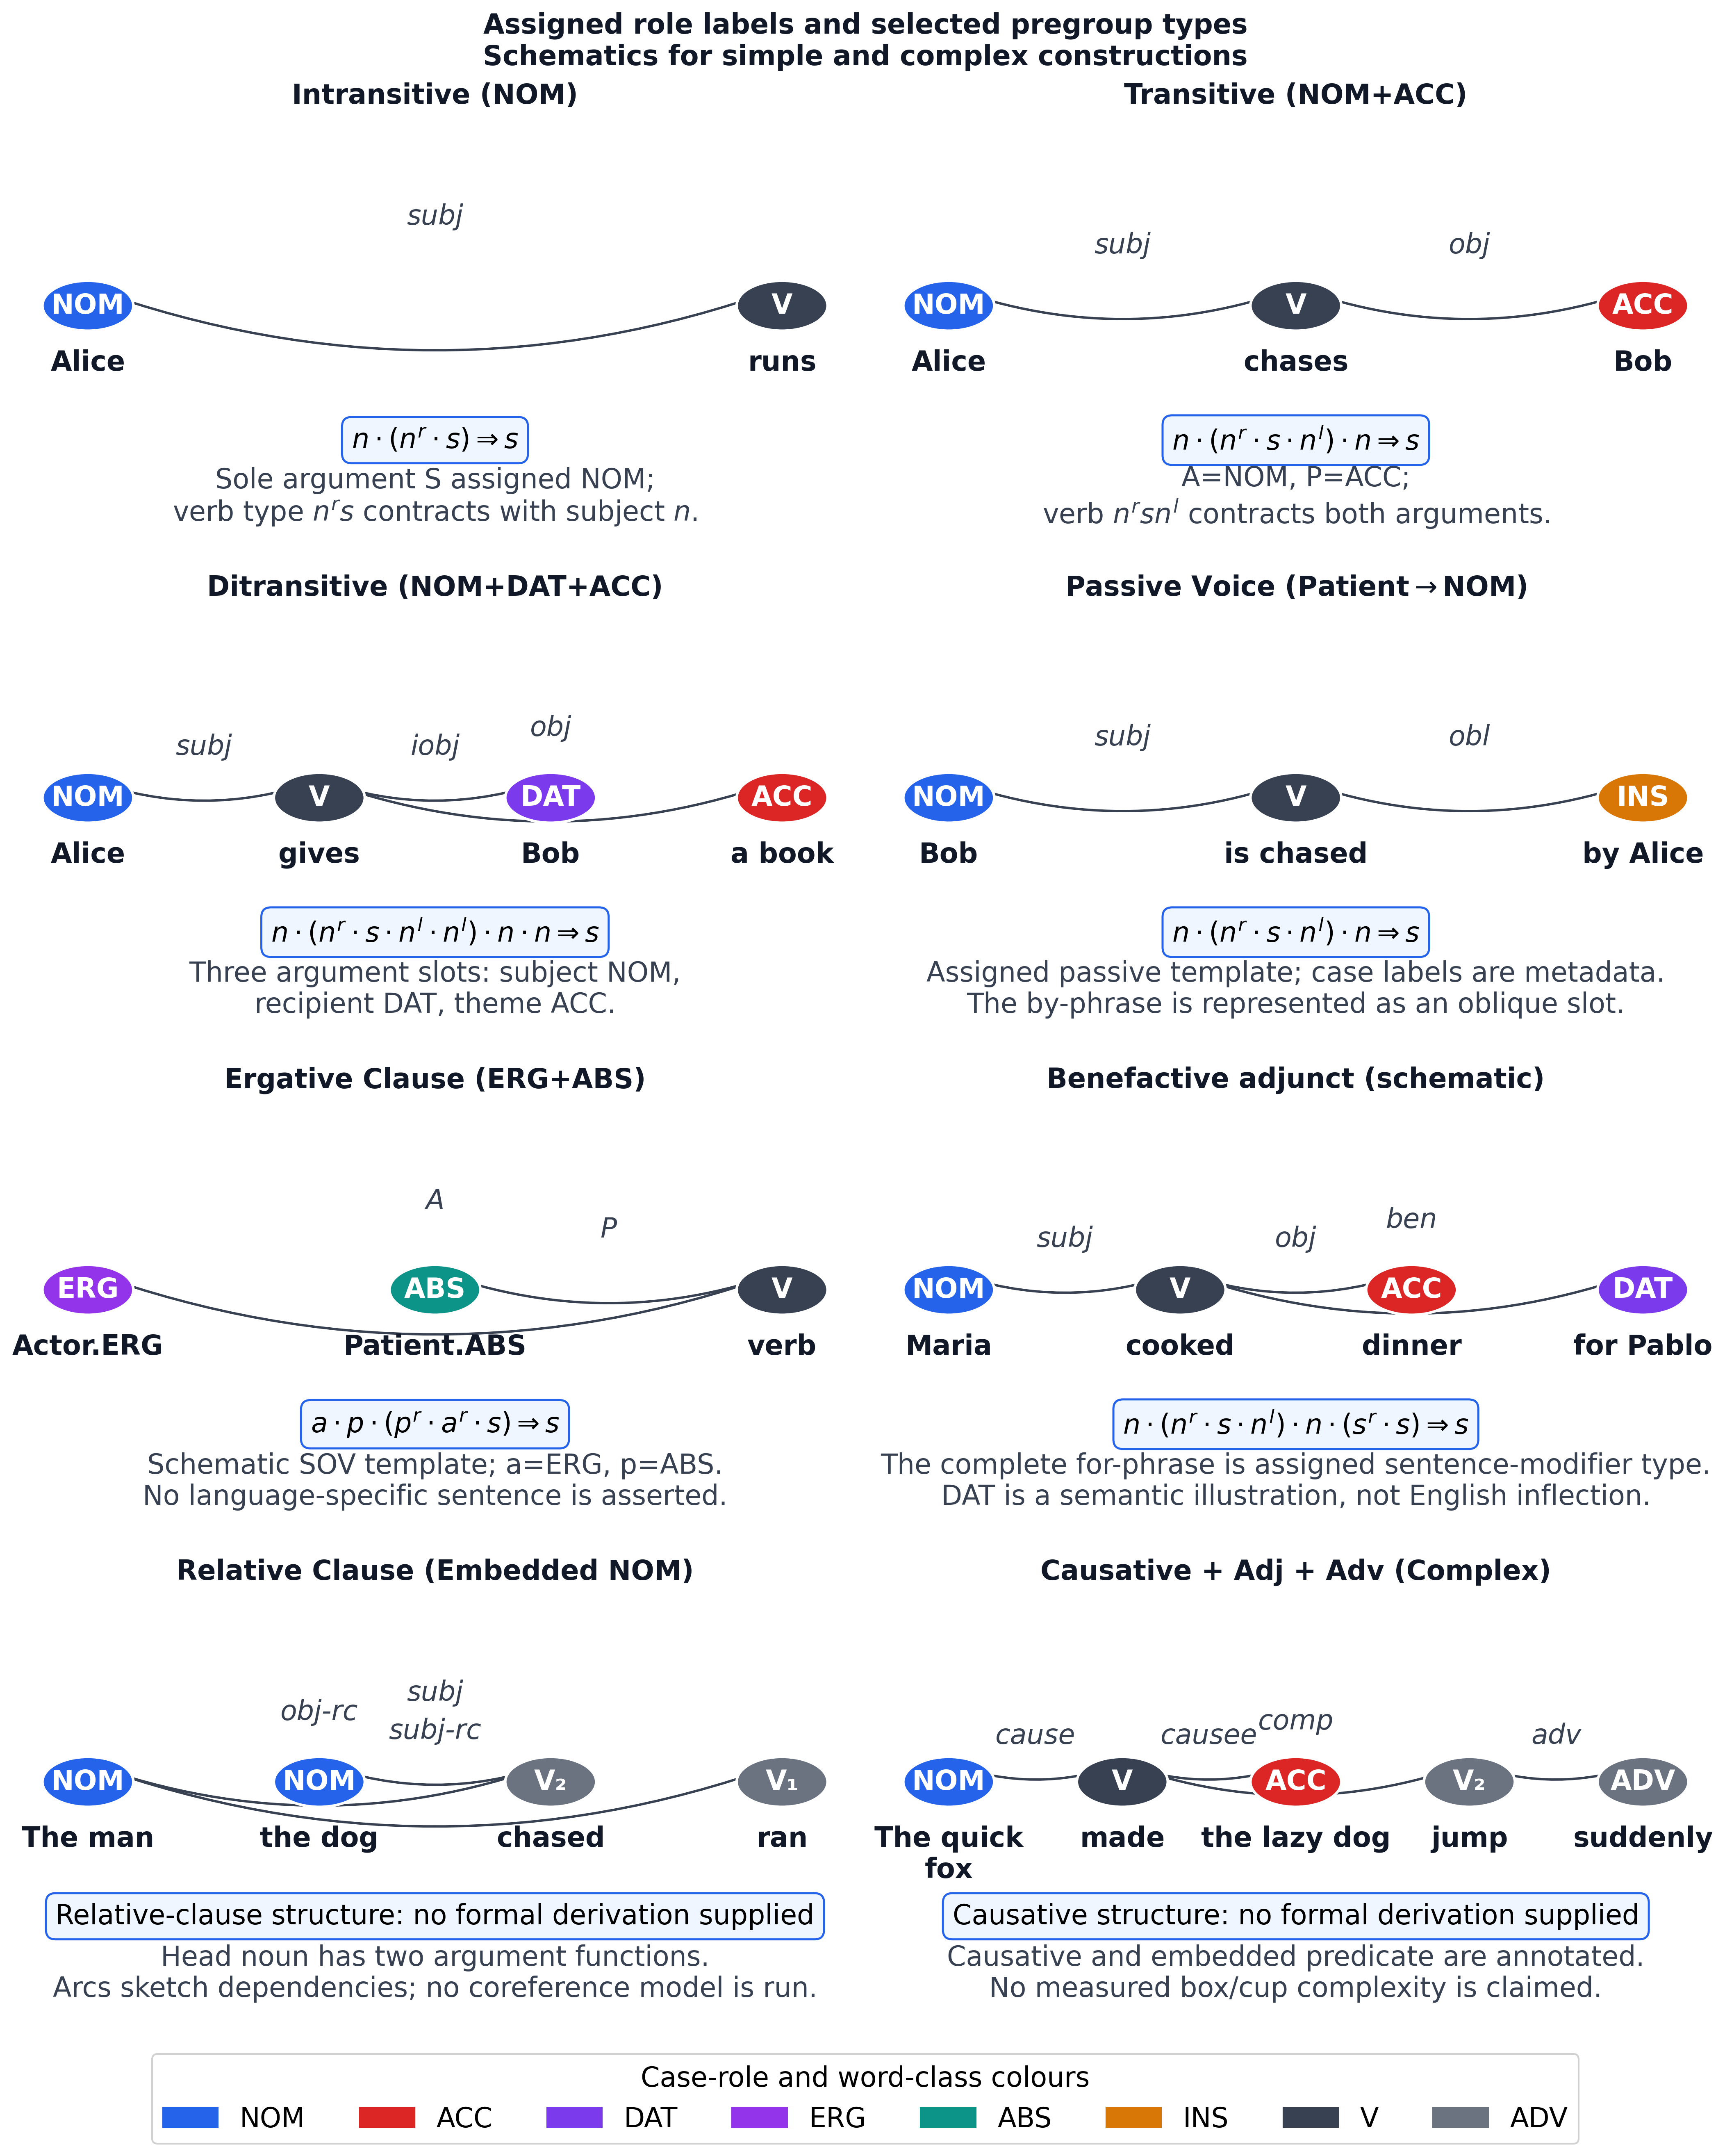
\includegraphics[keepaspectratio,alt={Compositional complexity increases monotonically from intransitive to causative constructions across eight case-assignment patterns. Multi-panel diagram ordered by categorical complexity \textbackslash kappa(D) (). Top of each panel: constituency-style syntactic tree with argument arcs and colour-coded case roles (Blue=NOM, Red=ACC, Violet=DAT, Purple=ERG, Teal=ABS, Dark=V). Bottom of each panel: categorical pregroup type formula showing Cup contractions that collapse argument wires to sentence type s. Panels 1--4 cover nominative-accusative (intransitive, transitive, ditransitive, passive); Panels 5--6 show ergative-absolutive and benefactive; Panels 7--8 demonstrate relative-clause embedding and causative complex predicates. Cup count and box count increase monotonically across panels, directly instantiating \textbackslash kappa(D). Generated programmatically from src.visualization.syntactic\_sentence\_diagrams.render\_syntactic\_panel().}]{../figures/syntactic_case_panel.png}}
\caption{Compositional complexity increases monotonically from
intransitive to causative constructions across eight case-assignment
patterns. Multi-panel diagram ordered by categorical complexity
\(\kappa(D)\) (\autoref{eq:eq-4-4}). \textbf{Top of each panel}:
constituency-style syntactic tree with argument arcs and colour-coded
case roles (Blue=NOM, Red=ACC, Violet=DAT, Purple=ERG, Teal=ABS,
Dark=V). \textbf{Bottom of each panel}: categorical pregroup type
formula showing Cup contractions that collapse argument wires to
sentence type \(s\). Panels 1--4 cover nominative-accusative
(intransitive, transitive, ditransitive, passive); Panels 5--6 show
ergative-absolutive and benefactive; Panels 7--8 demonstrate
relative-clause embedding and causative complex predicates. Cup count
and box count increase monotonically across panels, directly
instantiating \(\kappa(D)\). Generated programmatically from
\protect\texttt{src.visualization.syntactic\_sentence\_diagrams.render\_syntactic\_panel()}.}\label{fig:syntactic-panel}
\end{figure}

\newpage

\newpage

\section{Appendix B: Notation Reference}\label{sec:notation}

This appendix collects all notation, symbols, and technical terminology
used throughout the manuscript. Entries are grouped by domain and
ordered alphabetically within each section. The \textbf{First Use}
column indicates the section where each term is first introduced or
defined.

\textbf{Sections A--K:} A Linguistic Terms; B Category Theory; C
Enriched Categories and Magnitude; D Distributional Semantics and LLMs;
E Distributional Active Inference (DAIF); F Active Inference and
Cognitive Models; G Quantum and Topological Terms; H Logical and
Type-Theoretic Terms; I AI and Communication Protocols; J Diagrammatic
Reasoning; K Notation Conventions.

Figures that colour-code case roles (category graphs, string diagrams,
appendix panels) take those colours from the shared map
\texttt{CASE\_COLORS} in \texttt{src/visualization/styles.py} (keys are
\texttt{CaseRole} names). Captions state the mapping where it matters
for reading the diagram.

\subsection{Linguistic Terms}\label{sec:notation-linguistic}

\begin{longtable}[]{@{}
  >{\raggedright\arraybackslash}p{(\linewidth - 6\tabcolsep) * \real{0.1477}}
  >{\centering\arraybackslash}p{(\linewidth - 6\tabcolsep) * \real{0.0682}}
  >{\raggedright\arraybackslash}p{(\linewidth - 6\tabcolsep) * \real{0.7159}}
  >{\centering\arraybackslash}p{(\linewidth - 6\tabcolsep) * \real{0.0682}}@{}}
\caption{Linguistic terminology and
symbols.}\label{tbl:not-linguistic}\tabularnewline
\toprule\noalign{}
\begin{minipage}[b]{\linewidth}\raggedright
Term
\end{minipage} & \begin{minipage}[b]{\linewidth}\centering
Symbol
\end{minipage} & \begin{minipage}[b]{\linewidth}\raggedright
Definition
\end{minipage} & \begin{minipage}[b]{\linewidth}\centering
First Use
\end{minipage} \\
\midrule\noalign{}
\endfirsthead
\toprule\noalign{}
\begin{minipage}[b]{\linewidth}\raggedright
Term
\end{minipage} & \begin{minipage}[b]{\linewidth}\centering
Symbol
\end{minipage} & \begin{minipage}[b]{\linewidth}\raggedright
Definition
\end{minipage} & \begin{minipage}[b]{\linewidth}\centering
First Use
\end{minipage} \\
\midrule\noalign{}
\endhead
\bottomrule\noalign{}
\endlastfoot
Ablative & ABL & Case role encoding origin, source, or cause &
\href{02_case_systems.md\#sec:case-systems}{§2} \\
Accusative & ACC & Case role encoding patient, theme, or direct object &
\href{02_case_systems.md\#sec:case-systems}{§2} \\
Active--Stative alignment & --- & Alignment in which the sole argument S
splits by agentivity &
\href{02_case_systems.md\#sec:case-systems}{§2} \\
Agent-like argument & A & The agent-like argument of a transitive clause
& \href{02_case_systems.md\#sec:case-systems}{§2} \\
Alignment functor & \(F: \mathcal{U} \to \mathcal{L}\) &
Structure-preserving map from universal to language-specific case
category & \href{02_case_systems.md\#sec:case-systems}{§2} \\
Alignment type & --- & Systematic pattern governing how S, A, P are
grouped for case marking &
\href{02_case_systems.md\#sec:case-systems}{§2} \\
Case category & \(\mathcal{C}\) & Small category whose objects are case
roles and morphisms are grammatical relations &
\href{02_case_systems.md\#sec:case-systems}{§2} \\
Case frame & --- & The set of case roles activated by a particular verb
or predicate & \href{02_case_systems.md\#sec:case-systems}{§2} \\
Case-typed noun space & \(N_{\text{NOM}}, N_{\text{ACC}}, \ldots\) &
Case-specific vector subspace in a case-enriched DisCoCat model &
\href{04_categorical_semantics.md\#sec:categorical-semantics}{§4} \\
Categorial grammar & --- & Grammar assigning each lexical item an
algebraic type encoding combinatory potential &
\href{03_categorial_grammar.md\#sec:categorial-grammar}{§3} \\
Contraction & \(a^l \cdot a \to 1\) & Pregroup reduction eliminating an
adjoint pair &
\href{03_categorial_grammar.md\#sec:categorial-grammar}{§3} \\
Dative & DAT & Case role encoding recipient, goal, or beneficiary &
\href{02_case_systems.md\#sec:case-systems}{§2} \\
Deep case & --- & Fillmore's universal semantic primitive (e.g.,
Agentive, Objective) &
\href{02_case_systems.md\#sec:case-systems}{§2} \\
Ergative--Absolutive alignment & --- & Alignment grouping S = P \(\neq\)
A & \href{02_case_systems.md\#sec:case-systems}{§2} \\
Expansion & \(1 \to a \cdot a^l\) & Pregroup expansion introducing an
adjoint pair &
\href{03_categorial_grammar.md\#sec:categorial-grammar}{§3} \\
Fluid-S & --- & Alignment in which S marking varies by context or
volition & \href{02_case_systems.md\#sec:case-systems}{§2} \\
Fluid-S functor & \(F_\theta\) & Context-dependent alignment functor
parameterized by a volition feature \(\theta\) &
\href{02_case_systems.md\#sec:case-systems}{§2} \\
Functors (Alignment) & \(F_{\text{acc}}, F_{\text{erg}}\) & Alignment
functors \(\mathcal{U} \to \mathcal{L}_{\text{acc}}\)
resp.~\(\mathcal{U} \to \mathcal{L}_{\text{erg}}\) &
\href{02_case_systems.md\#sec:case-systems}{§2} \\
Language-specific case category &
\(\mathcal{L}_{\text{acc}}, \mathcal{L}_{\text{erg}}\) & Codomain
categories for accusative vs.~ergative alignment functors &
\href{02_case_systems.md\#sec:case-systems}{§2} \\
Genitive & GEN & Case role encoding possessor or source &
\href{02_case_systems.md\#sec:case-systems}{§2} \\
Formal semantics & --- & Montague's programme: meaning assigned
compositionally via truth-conditional functions &
\href{04_categorical_semantics.md\#sec:categorical-semantics}{§4} \\
Grammatical relation & --- & Morphism in a case category relating two
case roles & \href{02_case_systems.md\#sec:case-systems}{§2} \\
Instrumental & INS & Case role encoding instrument or means &
\href{02_case_systems.md\#sec:case-systems}{§2} \\
Kāraka & --- & Pāṇini's system of deep semantic roles in Sanskrit
grammar & \href{02_case_systems.md\#sec:case-systems}{§2} \\
Left adjoint & \(a^l\) & Left adjoint type satisfying
\(a^l \cdot a \leq 1\) &
\href{03_categorial_grammar.md\#sec:categorial-grammar}{§3} \\
Locative & LOC & Case role encoding location or context &
\href{02_case_systems.md\#sec:case-systems}{§2} \\
Markedness & --- & Asymmetry in the formal complexity of paradigmatic
oppositions & \href{02_case_systems.md\#sec:case-systems}{§2} \\
Monadic semantics & --- & Song's extension using monads to model
sublexical verb-root decomposition &
\href{03_categorial_grammar.md\#sec:categorial-grammar}{§3} \\
Nominative & NOM & Case role encoding agent, experiencer, or
intransitive subject &
\href{02_case_systems.md\#sec:case-systems}{§2} \\
Nominative--Accusative alignment & --- & Alignment grouping S = A
\(\neq\) P & \href{02_case_systems.md\#sec:case-systems}{§2} \\
Passivization & --- & Syntactic transformation promoting patient to
subject position &
\href{03_categorial_grammar.md\#sec:categorial-grammar}{§3} \\
Patient-like argument & P & The patient-like argument of a transitive
clause & \href{02_case_systems.md\#sec:case-systems}{§2} \\
Pregroup grammar & --- & Grammar where types have left and right
adjoints forming a compact closed category &
\href{03_categorial_grammar.md\#sec:categorial-grammar}{§3} \\
Proto-Agent & --- & Dowty's cluster of agentive entailments (volition,
sentience, causation) &
\href{02_case_systems.md\#sec:case-systems}{§2} \\
Proto-Patient & --- & Dowty's cluster of patient entailments (change of
state, causal affectedness) &
\href{02_case_systems.md\#sec:case-systems}{§2} \\
Right adjoint & \(a^r\) & Right adjoint type satisfying
\(a \cdot a^r \leq 1\) &
\href{03_categorial_grammar.md\#sec:categorial-grammar}{§3} \\
Sole argument & S & The sole argument of an intransitive clause &
\href{02_case_systems.md\#sec:case-systems}{§2} \\
Thematic role & --- & Semantic relation between a predicate and its
argument (Agent, Patient, Goal, etc.) &
\href{02_case_systems.md\#sec:case-systems}{§2} \\
Tripartite alignment & --- & Alignment in which S \(\neq\) A \(\neq\) P
(all three distinguished) &
\href{02_case_systems.md\#sec:case-systems}{§2} \\
Verb root decomposition & --- & Analysis of a verb's internal causative
and result-state layers via a monad &
\href{03_categorial_grammar.md\#sec:categorial-grammar}{§3} \\
Vocative & VOC & Case role encoding direct address &
\href{02_case_systems.md\#sec:case-systems}{§2} \\
\end{longtable}

\subsection{Category Theory}\label{sec:notation-category}

\begin{longtable}[]{@{}
  >{\raggedright\arraybackslash}p{(\linewidth - 6\tabcolsep) * \real{0.1477}}
  >{\centering\arraybackslash}p{(\linewidth - 6\tabcolsep) * \real{0.0682}}
  >{\raggedright\arraybackslash}p{(\linewidth - 6\tabcolsep) * \real{0.7159}}
  >{\centering\arraybackslash}p{(\linewidth - 6\tabcolsep) * \real{0.0682}}@{}}
\caption{Category theory terminology and
symbols.}\label{tbl:not-category}\tabularnewline
\toprule\noalign{}
\begin{minipage}[b]{\linewidth}\raggedright
Term
\end{minipage} & \begin{minipage}[b]{\linewidth}\centering
Symbol
\end{minipage} & \begin{minipage}[b]{\linewidth}\raggedright
Definition
\end{minipage} & \begin{minipage}[b]{\linewidth}\centering
First Use
\end{minipage} \\
\midrule\noalign{}
\endfirsthead
\toprule\noalign{}
\begin{minipage}[b]{\linewidth}\raggedright
Term
\end{minipage} & \begin{minipage}[b]{\linewidth}\centering
Symbol
\end{minipage} & \begin{minipage}[b]{\linewidth}\raggedright
Definition
\end{minipage} & \begin{minipage}[b]{\linewidth}\centering
First Use
\end{minipage} \\
\midrule\noalign{}
\endhead
\bottomrule\noalign{}
\endlastfoot
Box & --- & Node in a string diagram representing a morphism &
\href{03_categorial_grammar.md\#sec:categorial-grammar}{§3} \\
Cap & \(\eta: 1 \to a^r \otimes a\) & Unit of a compact closure
(coevaluation map) &
\href{03_categorial_grammar.md\#sec:categorial-grammar}{§3} \\
Category & \(\mathcal{C}\) & Collection of objects and morphisms with
identity and associative composition &
\href{02_case_systems.md\#sec:case-systems}{§2} \\
Classifying topos & \(\mathcal{E}_{\mathbb{T}}\) & Canonical topos:
models of \(\mathbb{T}\) in a Grothendieck topos \(\mathcal{F}\)
correspond to geometric morphisms
\(\mathcal{F} \to \mathcal{E}_{\mathbb{T}}\) &
\href{06_topos_theory.md\#sec:topos-theory}{§6} \\
Codomain & \(\text{cod}(f)\) & Target object of a morphism \(f\) &
\href{02_case_systems.md\#sec:case-systems}{§2} \\
Commutative diagram & --- & Diagram in which all directed paths with the
same start and end yield equal composites &
\href{01_introduction.md\#sec:introduction}{§1} \\
Cobordism & --- & Manifold with boundary connecting two
lower-dimensional manifolds; domain of TQFT functors &
\href{08_quantum_active_inference.md\#sec:quantum-active-inference}{§8} \\
Compact closed category & --- & Monoidal category in which every object
has a left and right dual &
\href{03_categorial_grammar.md\#sec:categorial-grammar}{§3} \\
Composition & \(g \circ f\) & Sequential application of morphisms: first
\(f\), then \(g\) & \href{02_case_systems.md\#sec:case-systems}{§2} \\
Cup & \(\varepsilon: a \otimes a^r \to 1\) & Counit of a compact closure
(evaluation map) &
\href{03_categorial_grammar.md\#sec:categorial-grammar}{§3} \\
Diagram & \(D\) & DisCoPy representation of a morphism in a monoidal
category &
\href{03_categorial_grammar.md\#sec:categorial-grammar}{§3} \\
\(\dagger\)-compact closed category & --- & Compact closed category with
a contravariant involutive endofunctor \(\dagger\); framework for
ZX-calculus &
\href{08_quantum_active_inference.md\#sec:quantum-active-inference}{§8} \\
Domain & \(\text{dom}(f)\) & Source object of a morphism \(f\) &
\href{02_case_systems.md\#sec:case-systems}{§2} \\
Fiber bundle & --- & Projection \(\pi: E \to B\) whose fibers carry
role-filler structure; topos-theoretic LoT model &
\href{06_topos_theory.md\#sec:topos-theory}{§6} \\
Functor & \(F: \mathcal{C} \to \mathcal{D}\) & Structure-preserving map
between categories & \href{02_case_systems.md\#sec:case-systems}{§2} \\
Geometric theory & \(\mathbb{T}\) & Theory axiomatized by sequents with
finite conjunctions, arbitrary disjunctions, existential quantification
& \href{06_topos_theory.md\#sec:topos-theory}{§6} \\
Geometric theories (case) &
\(\mathbb{T}_{\text{typ}}, \mathbb{T}_{\text{log}}, \mathbb{T}_{\text{dist}}, \mathbb{T}_{\text{enr}}\)
& Typological, type-logical, distributional (DisCoCat), and enriched
case theories (\autoref{sec:topos-theory}) &
\href{06_topos_theory.md\#sec:topos-theory}{§6} \\
Bridge topos & \(\mathcal{E}_{\mathbb{T}_{\text{bridge}}}\) (schematic)
& Intermediate classifying topos linking two formalizations in the
Morita bridge programme &
\href{06_topos_theory.md\#sec:topos-theory}{§6} \\
Identity morphism & \(\text{id}_A\) & Morphism from \(A\) to itself
satisfying \(f \circ \text{id} = f = \text{id} \circ f\) &
\href{02_case_systems.md\#sec:case-systems}{§2} \\
Monad & --- & Endofunctor with unit and multiplication satisfying
associativity and unit laws &
\href{03_categorial_grammar.md\#sec:categorial-grammar}{§3} \\
Monoidal category & --- & Category with a bifunctor \(\otimes\) (tensor
product) and unit object \(I\) &
\href{03_categorial_grammar.md\#sec:categorial-grammar}{§3} \\
Morita equivalence &
\(\mathcal{E}_{\mathbb{T}_1} \simeq \mathcal{E}_{\mathbb{T}_2}\) &
Equivalence of classifying toposes enabling inter-theoretic transfer &
\href{06_topos_theory.md\#sec:topos-theory}{§6} \\
Morphism & \(f: A \to B\) & Arrow between objects in a category; encodes
a relation or transformation &
\href{02_case_systems.md\#sec:case-systems}{§2} \\
Natural transformation & \(\alpha: F \Rightarrow G\) & Family of
morphisms \(\alpha_A: F(A) \to G(A)\) commuting with all morphisms;
alignment maps in semantics use \(\nu_{\text{acc}}, \nu_{\text{erg}}\);
compact-closure cap \(\eta_{\mathrm{cc}}\) is distinct from IQN
curvature \(\eta_{\mathrm{IQN}}\) &
\href{02_case_systems.md\#sec:case-systems}{§2} \\
Object & \(A, B, \ldots\) & Entities in a category; in our framework,
case roles & \href{02_case_systems.md\#sec:case-systems}{§2} \\
Presheaf & \(\hat{\mathcal{C}} = [\mathcal{C}^{op}, \textbf{Set}]\) &
Contravariant functor from \(\mathcal{C}\) to \textbf{Set} &
\href{06_topos_theory.md\#sec:topos-theory}{§6} \\
Snake equation & \((1 \otimes \varepsilon) \circ (\eta \otimes 1) = 1\)
& Zigzag identity: fundamental axiom of compact closed categories &
\href{04_categorical_semantics.md\#sec:categorical-semantics}{§4} \\
String diagram & --- & Planar graph faithfully representing morphisms in
a monoidal category &
\href{03_categorial_grammar.md\#sec:categorial-grammar}{§3} \\
Subobject classifier & \(\Omega\) & Object in a topos playing the role
of a truth-value object &
\href{06_topos_theory.md\#sec:topos-theory}{§6} \\
Swap & \(\sigma_{A,B}: A \otimes B \to B \otimes A\) & Braiding morphism
permuting two objects in a symmetric monoidal category &
\href{03_categorial_grammar.md\#sec:categorial-grammar}{§3} \\
Tensor product & \(A \otimes B\) & Monoidal product representing
parallel composition or concatenation &
\href{03_categorial_grammar.md\#sec:categorial-grammar}{§3} \\
Topos & \(\mathcal{E}\) & Category with products, exponentials, and a
subobject classifier; generalized universe of sets &
\href{06_topos_theory.md\#sec:topos-theory}{§6} \\
Universal construction & --- & Object or morphism characterized by a
universal property (product, coproduct, limit) &
\href{06_topos_theory.md\#sec:topos-theory}{§6} \\
Wire & --- & Edge in a string diagram representing a type (object) &
\href{03_categorial_grammar.md\#sec:categorial-grammar}{§3} \\
\end{longtable}

\subsection{Enriched Categories and
Magnitude}\label{sec:notation-enriched}

\begin{longtable}[]{@{}
  >{\raggedright\arraybackslash}p{(\linewidth - 6\tabcolsep) * \real{0.1477}}
  >{\centering\arraybackslash}p{(\linewidth - 6\tabcolsep) * \real{0.0682}}
  >{\raggedright\arraybackslash}p{(\linewidth - 6\tabcolsep) * \real{0.7159}}
  >{\centering\arraybackslash}p{(\linewidth - 6\tabcolsep) * \real{0.0682}}@{}}
\caption{Enriched categories and magnitude
terminology.}\label{tbl:not-enriched}\tabularnewline
\toprule\noalign{}
\begin{minipage}[b]{\linewidth}\raggedright
Term
\end{minipage} & \begin{minipage}[b]{\linewidth}\centering
Symbol
\end{minipage} & \begin{minipage}[b]{\linewidth}\raggedright
Definition
\end{minipage} & \begin{minipage}[b]{\linewidth}\centering
First Use
\end{minipage} \\
\midrule\noalign{}
\endfirsthead
\toprule\noalign{}
\begin{minipage}[b]{\linewidth}\raggedright
Term
\end{minipage} & \begin{minipage}[b]{\linewidth}\centering
Symbol
\end{minipage} & \begin{minipage}[b]{\linewidth}\raggedright
Definition
\end{minipage} & \begin{minipage}[b]{\linewidth}\centering
First Use
\end{minipage} \\
\midrule\noalign{}
\endhead
\bottomrule\noalign{}
\endlastfoot
Base-change functor & --- & Conceptual tower
\(\mathbf{Bool} \hookrightarrow [0,1] \hookrightarrow \mathbf{R}_{\geq 0}\)
showing progressively richer enrichments of grammatical categories (not
computationally instantiated; this paper implements only
\([0,1]\)-enrichment) &
\href{03_categorial_grammar.md\#sec:categorial-grammar}{§3} \\
Categorical magnitude & \(\lvert X \rvert\) & Sum \(\sum_i w_i\) where
\((w_1, \ldots, w_n)\) solves \(Z \mathbf{w} = \mathbf{1}\); measures
effective number of objects &
\href{05_enriched_categories.md\#sec:enriched-categories}{§5} \\
Composition inequality &
\(\mathcal{V}(A,B) \cdot \mathcal{V}(B,C) \leq \mathcal{V}(A,C)\) &
Enriched analogue of composition on \(([0,1], \cdot, 1)\): composite
hom-value is at least the product of intermediates &
\href{05_enriched_categories.md\#sec:enriched-categories}{§5} \\
Enriched category & \(\mathcal{V}\text{-Cat}\) & Category whose hom-sets
are replaced by objects of a monoidal category \(\mathcal{V}\) &
\href{05_enriched_categories.md\#sec:enriched-categories}{§5} \\
Enriched functor & --- & Structure-preserving map between enriched
categories respecting hom-values &
\href{05_enriched_categories.md\#sec:enriched-categories}{§5} \\
Hom-value & \(\mathcal{V}(A,B) \in [0,1]\) & Enriched analogue of
hom-set; measures degree of relation between objects &
\href{05_enriched_categories.md\#sec:enriched-categories}{§5} \\
Identity axiom & \(\mathcal{V}(A,A) = 1\) & Every object has maximal
self-relatedness in the enriched hom (equality, not mere inequality, in
our \([0,1]\)-convention) &
\href{05_enriched_categories.md\#sec:enriched-categories}{§5} \\
Similarity matrix & \(Z_{ij} = \mathcal{V}(A_i, A_j)\) & Matrix of all
pairwise hom-values; used to compute categorical magnitude &
\href{05_enriched_categories.md\#sec:enriched-categories}{§5} \\
Lawvere metric space & --- & Category enriched over
\(([0,\infty], +, 0)\); generalizes metric spaces via enriched
categories &
\href{05_enriched_categories.md\#sec:enriched-categories}{§5} \\
Magnitude homology & \(\text{MH}_n(\mathcal{C})\) & Graded homological
invariant categorifying magnitude; detects higher-dimensional holes in
enriched categories &
\href{05_enriched_categories.md\#sec:enriched-categories}{§5} \\
Morphism weight (precision) & \(w_f\), \(w_k\), \(w_c\) & Enriched
weights in \([0,1]\); subscript denotes morphism or role in VMP/DPE
(\autoref{sec:daif-results}). \textbf{Convention}: \(w_f\) always refers
to the \emph{enriched} hom-value \(\mathcal{C}(A,B)\) in the
\([0,1]\)-enriched category
(\href{05_enriched_categories.md\#sec:enriched-categories}{§5}), not the
unit-weight morphism scalar carried by the \texttt{CaseCategory} in
\href{02_case_systems.md\#sec:case-systems}{§2} --- the two number
systems are intentionally decoupled in the implementation (see
\href{05_enriched_categories.md\#sec:enriched-categories}{§5}
Architectural note). &
\href{07_cognitive_integration.md\#sec:cognitive-integration}{§7} \\
POVM element & \(E_c\) & Positive operator-valued measure element for
case role \(c\); \(P(c \mid \rho) = \text{Tr}(E_c \rho)\) &
\href{08_quantum_active_inference.md\#sec:quantum-active-inference}{§8} \\
Prediction error & \(\text{PE}(f)\) &
\(\propto w_f \cdot \lvert\mu_{\text{predicted}} - \mu_{\text{observed}}\rvert\);
case violation signal scaling with morphism weight &
\href{07_cognitive_integration.md\#sec:cognitive-integration}{§7} \\
Shannon entropy & \(H\) & Information-theoretic measure characterized as
the unique derivation of a topological operad (Bradley) &
\href{05_enriched_categories.md\#sec:enriched-categories}{§5} \\
Topological operad & --- & Operad with topological structure whose
derivations connect magnitude to entropy &
\href{05_enriched_categories.md\#sec:enriched-categories}{§5} \\
Weight vector & \(\mathbf{w}\) & Solution to
\(Z\mathbf{w} = \mathbf{1}\); entries are the effective weights of each
object &
\href{05_enriched_categories.md\#sec:enriched-categories}{§5} \\
\end{longtable}

\subsection{Distributional Semantics and
LLMs}\label{sec:notation-distributional}

\begin{longtable}[]{@{}
  >{\raggedright\arraybackslash}p{(\linewidth - 6\tabcolsep) * \real{0.1477}}
  >{\centering\arraybackslash}p{(\linewidth - 6\tabcolsep) * \real{0.0682}}
  >{\raggedright\arraybackslash}p{(\linewidth - 6\tabcolsep) * \real{0.7159}}
  >{\centering\arraybackslash}p{(\linewidth - 6\tabcolsep) * \real{0.0682}}@{}}
\caption{Distributional semantics and LLM
terminology.}\label{tbl:not-distributional}\tabularnewline
\toprule\noalign{}
\begin{minipage}[b]{\linewidth}\raggedright
Term
\end{minipage} & \begin{minipage}[b]{\linewidth}\centering
Symbol
\end{minipage} & \begin{minipage}[b]{\linewidth}\raggedright
Definition
\end{minipage} & \begin{minipage}[b]{\linewidth}\centering
First Use
\end{minipage} \\
\midrule\noalign{}
\endfirsthead
\toprule\noalign{}
\begin{minipage}[b]{\linewidth}\raggedright
Term
\end{minipage} & \begin{minipage}[b]{\linewidth}\centering
Symbol
\end{minipage} & \begin{minipage}[b]{\linewidth}\raggedright
Definition
\end{minipage} & \begin{minipage}[b]{\linewidth}\centering
First Use
\end{minipage} \\
\midrule\noalign{}
\endhead
\bottomrule\noalign{}
\endlastfoot
Attention mechanism & --- & Transformer component computing weighted
relevance between token positions &
\href{04_categorical_semantics.md\#sec:categorical-semantics}{§4} \\
Attention weight & \(\alpha_{ij}\) & Softmax-normalized score encoding
contextual relevance of token \(j\) to token \(i\) &
\href{04_categorical_semantics.md\#sec:categorical-semantics}{§4} \\
BERT & --- & Bidirectional Encoder Representations from Transformers;
masked language model producing contextualized embeddings &
\href{04_categorical_semantics.md\#sec:categorical-semantics}{§4} \\
Contextualized embedding & \(\mathbf{v}_w^{(c)}\) & Vector
representation of word \(w\) that varies with linguistic context \(c\) &
\href{04_categorical_semantics.md\#sec:categorical-semantics}{§4} \\
Compact closure map & \(\varepsilon_N: N \otimes N \to \mathbb{R}\) &
Inner product implementing pregroup contraction in the vector space
semantics &
\href{04_categorical_semantics.md\#sec:categorical-semantics}{§4} \\
Cosine similarity & \(\cos(\mathbf{u}, \mathbf{v})\) & Similarity
measure
\(\frac{\mathbf{u} \cdot \mathbf{v}}{\|\mathbf{u}\| \|\mathbf{v}\|}\)
between vectors &
\href{05_enriched_categories.md\#sec:enriched-categories}{§5} \\
Distributional Memory & --- & Baroni--Lenci tensor-based framework
structuring co-occurrence as (word, relation, word) triples &
\href{04_categorical_semantics.md\#sec:categorical-semantics}{§4} \\
DisCoCat & --- & Distributional Compositional Categorical model;
monoidal functor from pregroup grammars to vector spaces &
\href{03_categorial_grammar.md\#sec:categorial-grammar}{§3} \\
DisCoCirc & --- & Discourse-level extension of DisCoCat with persistent
entity wires &
\href{04_categorical_semantics.md\#sec:categorical-semantics}{§4} \\
Distributional hypothesis & --- & The thesis that words occurring in
similar contexts have similar meanings (Harris 1954, Firth 1957) &
\href{04_categorical_semantics.md\#sec:categorical-semantics}{§4} \\
GloVe & --- & Global Vectors for Word Representation; log-bilinear model
of word co-occurrence statistics &
\href{04_categorical_semantics.md\#sec:categorical-semantics}{§4} \\
GPT & --- & Generative Pre-trained Transformer; autoregressive language
model &
\href{04_categorical_semantics.md\#sec:categorical-semantics}{§4} \\
Meaning functor & \(F: \mathbf{Preg} \to \mathbf{FVect}\) & Monoidal
functor assigning vector spaces to types and linear maps to derivations
& \href{04_categorical_semantics.md\#sec:categorical-semantics}{§4} \\
Noun space & \(N\) & Vector space to which noun types \(n\) map under
the meaning functor &
\href{04_categorical_semantics.md\#sec:categorical-semantics}{§4} \\
Parameterized optic & --- & Categorical construction (Gavranović)
modeling attention heads as functorial lenses &
\href{09_ai_implications.md\#sec:ai-implications}{§9} \\
Self-attention &
\(\text{Attn}(Q,K,V) = \mathrm{softmax}(\frac{QK^\top}{\sqrt{d_k}})V\) &
Core transformer operation computing contextualized representations &
\href{04_categorical_semantics.md\#sec:categorical-semantics}{§4} \\
Sentence space & \(S\) & Vector space to which sentence type \(s\) maps
under the meaning functor &
\href{04_categorical_semantics.md\#sec:categorical-semantics}{§4} \\
Sentence vector & \(\overrightarrow{\text{sentence}}\) & Vector in \(S\)
computed by tensoring and contracting word meanings via DisCoCat &
\href{04_categorical_semantics.md\#sec:categorical-semantics}{§4} \\
Static embedding & \(\mathbf{v}_w\) & Fixed vector representation of
word \(w\) independent of context (e.g., Word2Vec, GloVe) &
\href{04_categorical_semantics.md\#sec:categorical-semantics}{§4} \\
Transformer & --- & Neural architecture using self-attention and
feed-forward layers for sequence processing &
\href{04_categorical_semantics.md\#sec:categorical-semantics}{§4} \\
Word2Vec & --- & Neural embedding model (Mikolov et al.~2013) learning
word vectors from local context windows &
\href{04_categorical_semantics.md\#sec:categorical-semantics}{§4} \\
Word vector & \(\mathbf{v}_w \in \mathbb{R}^d\) & \(d\)-dimensional
real-valued vector encoding distributional properties of word \(w\) &
\href{04_categorical_semantics.md\#sec:categorical-semantics}{§4} \\
\end{longtable}

\subsection{Distributional Active Inference
(DAIF)}\label{sec:notation-daif}

\begin{longtable}[]{@{}
  >{\raggedright\arraybackslash}p{(\linewidth - 6\tabcolsep) * \real{0.1477}}
  >{\centering\arraybackslash}p{(\linewidth - 6\tabcolsep) * \real{0.0682}}
  >{\raggedright\arraybackslash}p{(\linewidth - 6\tabcolsep) * \real{0.7159}}
  >{\centering\arraybackslash}p{(\linewidth - 6\tabcolsep) * \real{0.0682}}@{}}
\caption{Distributional Active Inference (DAIF)
terminology.}\label{tbl:not-daif}\tabularnewline
\toprule\noalign{}
\begin{minipage}[b]{\linewidth}\raggedright
Term
\end{minipage} & \begin{minipage}[b]{\linewidth}\centering
Symbol
\end{minipage} & \begin{minipage}[b]{\linewidth}\raggedright
Definition
\end{minipage} & \begin{minipage}[b]{\linewidth}\centering
First Use
\end{minipage} \\
\midrule\noalign{}
\endfirsthead
\toprule\noalign{}
\begin{minipage}[b]{\linewidth}\raggedright
Term
\end{minipage} & \begin{minipage}[b]{\linewidth}\centering
Symbol
\end{minipage} & \begin{minipage}[b]{\linewidth}\raggedright
Definition
\end{minipage} & \begin{minipage}[b]{\linewidth}\centering
First Use
\end{minipage} \\
\midrule\noalign{}
\endhead
\bottomrule\noalign{}
\endlastfoot
Return distribution & \(Z(s,a)\) & Full probability distribution over
discounted cumulative rewards from state \(s\) under action \(a\) &
\href{07c_daif_results.md\#sec:daif-results}{§7c} \\
Distributional Bellman operator & \(\mathcal{T}^{\pi}\) & Distributional
analogue of the Bellman operator:
\(\mathcal{T}^{\pi}Z \stackrel{d}{=} R + \gamma Z'\) &
\href{07c_daif_results.md\#sec:daif-results}{§7c} \\
Push-forward measure & \(\mathbf{S}_{\#}\mathbb{P}\) & Path-level
push-forward of the trajectory measure (composed with decoder
\(f: \mathcal{S} \to \mathcal{X}\) in \autoref{eq:eq-7-1}); generic
push-forward written \(T_{\#}\mu\) &
\href{07c_daif_results.md\#sec:daif-results}{§7c} \\
Discount factor & \(\gamma \in (0,1)\) & Exponential time-discount in
the distributional Bellman return &
\href{07c_daif_results.md\#sec:daif-results}{§7c} \\
Quantile level & \(\tau \in [0,1]\) & Quantile index in QR-DQN and IQN;
sampled uniformly at inference time &
\href{07c_daif_results.md\#sec:daif-results}{§7c} \\
Quantile Huber loss & \(\rho_{\tau}^{\kappa}{(u)}\) & Loss function for
quantile regression: interpolates \(L^1\) and \(L^2\) via threshold
\(\kappa{}\) & \href{07c_daif_results.md\#sec:daif-results}{§7c} \\
Wasserstein distance & \(W_p(P,Q)\) & \(p\)-Wasserstein distance between
return distributions; \(W_1\) = area between CDFs &
\href{07c_daif_results.md\#sec:daif-results}{§7c} \\
Bethe free energy & \(F_{\text{Bethe}}[\mathbf{q}]\) & Tractable
approximation to variational free energy in belief propagation &
\href{07c_daif_results.md\#sec:daif-results}{§7c} \\
Expected information gain & \(\text{EIG}{(o)}\) &
\(D_{\mathrm{KL}}{(q{(\mathbf{c} \mid o)} \Vert p{(\mathbf{c})})}\);
epistemic value of observation \(o{}\) &
\href{07c_daif_results.md\#sec:daif-results}{§7c} \\
Expected free energy & \(G{(\pi)}\) & Pragmatic + epistemic + risk cost
of policy \(\pi{}\); minimised for action selection &
\href{07c_daif_results.md\#sec:daif-results}{§7c} \\
Distributional prediction error & \(\mathrm{DPE}\) & Precision-weighted
Wasserstein mismatch:
\(w_f \cdot W_1{(Z_{\text{pred}}, Z_{\text{obs}})}\) &
\href{07c_daif_results.md\#sec:daif-results}{§7c} \\
ERP amplitude profile & \(\mathrm{ERPProfile}\) & Dataclass holding
N400/P600 amplitudes, peak latencies, and time-series waveforms for each
case role & \href{07c_daif_results.md\#sec:daif-results}{§7c} \\
Return entropy & \(H[Z]\) & Shannon entropy of the return distribution:
\(-\sum_i p_i \log p_i\) &
\href{07c_daif_results.md\#sec:daif-results}{§7c} \\
Quantile calibration error & \(\mathrm{CE}\) & Mean absolute deviation
between nominal quantile levels and empirical coverage &
\href{07c_daif_results.md\#sec:daif-results}{§7c} \\
IQN risk distortion & \(\psi_{\mathrm{IQN}}(\tau)\) & Maps quantile
levels \(\tau{}\); piecewise formulas (neutral, power, tail, CVaR) match
\texttt{implicit\_quantile\_network\_update()} and the
\href{07c_daif_results.md\#sec:daif-results}{§7c} table; distinct from
\(\beta_{\mathrm{risk}}\) in \(G(\pi)\) &
\href{07c_daif_results.md\#sec:daif-results}{§7c} \\
IQN curvature & \(\eta_{\mathrm{IQN}}\) & Default \(0.71\) in code; not
the compact-closure cap \(\eta_{\mathrm{cc}}\) &
\href{07c_daif_results.md\#sec:daif-results}{§7c} \\
CVaR scale & \(\alpha_{\mathrm{CVaR}}\) & IQN mode uses
\(\psi_{\mathrm{IQN}}(\tau)=\tau\cdot\alpha_{\mathrm{CVaR}}\); default
\(0.25\) in code (distinct from softmax \(\alpha_{\mathrm{pol}}\)) &
\href{07c_daif_results.md\#sec:daif-results}{§7c} \\
Risk sensitivity (EFE) & \(\beta_{\mathrm{risk}}\) & Non-negative
coefficient on \(\text{risk}(\pi)\) in \(G(\pi)\);
\(\beta_{\mathrm{risk}}=0\) recovers standard EFE &
\href{07c_daif_results.md\#sec:daif-results}{§7c} \\
Inverse temperature (policy) & \(\alpha_{\mathrm{pol}}\) & Softmax
sharpness over policies in \(P(\pi)\) &
\href{07c_daif_results.md\#sec:daif-results}{§7c} \\
Belief precision (VMP) &
\(\Lambda_{\text{post}}, \Lambda_{\text{prior}}, \Lambda_{\text{lik}}\)
& Posterior, prior, and likelihood precision matrices; \(\Delta\Lambda\)
is their positive update magnitude &
\href{07c_daif_results.md\#sec:daif-results}{§7c} \\
Violation severity & \(S_{\text{violation}}\) & \(\in \{0, 0.5, 1.0\}\)
in ERP decomposition &
\href{07c_daif_results.md\#sec:daif-results}{§7c} \\
TD error (quantile) & \(\delta_{ij}\) & Temporal-difference residual in
QR-DQN (\autoref{eq:eq-7c-qr}) &
\href{07c_daif_results.md\#sec:daif-results}{§7c} \\
Quantile count (current) & \(N\) & Number of current-network quantile
levels in QR-DQN (Eq. \ref{eq:eq-7c-qr}); equal to the length of
\texttt{current\_quantiles} passed to \texttt{quantile\_td\_update()} &
\href{07c_daif_results.md\#sec:daif-results}{§7c} \\
Quantile count (target) & \(N'\) & Number of target-network quantile
samples in QR-DQN (Eq. \ref{eq:eq-7c-qr}) &
\href{07c_daif_results.md\#sec:daif-results}{§7c} \\
Huber threshold & \(\kappa\) & Cut-point between quadratic and linear
regimes of the Huber loss \(L_\kappa(u)\) (Eq. \ref{eq:eq-7c-huber});
default \(\kappa=1\) in \texttt{quantile\_td\_update()} &
\href{07c_daif_results.md\#sec:daif-results}{§7c} \\
Atom count (C51) & \(N_{\text{atoms}}\) & Number of support atoms
\(z_i\) in the C51 categorical representation (Eq. \ref{eq:eq-7c-c51});
default \(N_{\text{atoms}}=51\) in
\texttt{categorical\_return\_distribution()} &
\href{07c_daif_results.md\#sec:daif-results}{§7c} \\
Support bounds (C51) & \(V_{\min},\,V_{\max}\) & Lower and upper
endpoints of the atomic support spanned by \(\{z_i\}\) in the C51
representation & \href{07c_daif_results.md\#sec:daif-results}{§7c} \\
Bin count (entropy) & \(N_{\text{bins}}\) & Number of equal-width bins
used to discretise the quantile-parameterised return when computing
\(H[Z]\) (Eq. \ref{eq:eq-7c-entropy}); default \(N_{\text{bins}}=50\) in
\texttt{return\_distribution\_entropy()} &
\href{07c_daif_results.md\#sec:daif-results}{§7c} \\
\end{longtable}

\subsection{Active Inference and Cognitive
Models}\label{sec:notation-cognitive}

\begin{longtable}[]{@{}
  >{\raggedright\arraybackslash}p{(\linewidth - 6\tabcolsep) * \real{0.1477}}
  >{\centering\arraybackslash}p{(\linewidth - 6\tabcolsep) * \real{0.0682}}
  >{\raggedright\arraybackslash}p{(\linewidth - 6\tabcolsep) * \real{0.7159}}
  >{\centering\arraybackslash}p{(\linewidth - 6\tabcolsep) * \real{0.0682}}@{}}
\caption{Active inference and cognitive modeling
terminology.}\label{tbl:not-cognitive}\tabularnewline
\toprule\noalign{}
\begin{minipage}[b]{\linewidth}\raggedright
Term
\end{minipage} & \begin{minipage}[b]{\linewidth}\centering
Symbol
\end{minipage} & \begin{minipage}[b]{\linewidth}\raggedright
Definition
\end{minipage} & \begin{minipage}[b]{\linewidth}\centering
First Use
\end{minipage} \\
\midrule\noalign{}
\endfirsthead
\toprule\noalign{}
\begin{minipage}[b]{\linewidth}\raggedright
Term
\end{minipage} & \begin{minipage}[b]{\linewidth}\centering
Symbol
\end{minipage} & \begin{minipage}[b]{\linewidth}\raggedright
Definition
\end{minipage} & \begin{minipage}[b]{\linewidth}\centering
First Use
\end{minipage} \\
\midrule\noalign{}
\endhead
\bottomrule\noalign{}
\endlastfoot
Active inference & --- & Framework in which perception and action are
unified as variational free energy minimization &
\href{07_cognitive_integration.md\#sec:cognitive-integration}{§7} \\
Active sampling & --- & Agent's selection of actions to confirm or
update case assignments via sensory evidence &
\href{07_cognitive_integration.md\#sec:cognitive-integration}{§7} \\
Belief updating & --- & Bayesian posterior computation: revising
generative model parameters given new observations &
\href{07_cognitive_integration.md\#sec:cognitive-integration}{§7} \\
CEREBRUM & --- & Case-Enabled Reasoning Engine with Bayesian
Representations for Unified Modeling; treats AI models as case-bearing
entities &
\href{07_cognitive_integration.md\#sec:cognitive-integration}{§7} \\
Distributional Active Inference (DAIF) & --- & Extension replacing
scalar value summaries with full return distributions in active
inference &
\href{07_cognitive_integration.md\#sec:cognitive-integration}{§7} \\
Distributional RL & --- & Reinforcement learning operating on full
return distributions rather than scalar expected values &
\href{07_cognitive_integration.md\#sec:cognitive-integration}{§7} \\
Free energy & \(F\) & Variational bound on surprisal;
\(F = D_{KL}[q(\theta) \parallel p(\theta \mid o)] - \ln p(o)\) &
\href{07_cognitive_integration.md\#sec:cognitive-integration}{§7} \\
Free energy principle (FEP) & --- & The principle that self-organizing
systems maintain themselves by minimizing surprisal &
\href{07_cognitive_integration.md\#sec:cognitive-integration}{§7} \\
Garden-path reanalysis & --- & Restructuring of case assignments when
incoming evidence contradicts the current parse &
\href{07_cognitive_integration.md\#sec:cognitive-integration}{§7} \\
Generative model & \(p(o, s)\) & Joint probability model over
observations \(o\) and hidden states \(s\) &
\href{07_cognitive_integration.md\#sec:cognitive-integration}{§7} \\
Markov blanket & --- & Statistical boundary separating internal states
from external environment; defines agent boundary &
\href{07_cognitive_integration.md\#sec:cognitive-integration}{§7} \\
N400 & --- & Event-related brain potential peaking \textasciitilde400ms
post-stimulus; indexes semantic prediction error &
\href{07_cognitive_integration.md\#sec:cognitive-integration}{§7} \\
P600 & --- & Event-related brain potential peaking \textasciitilde600ms
post-stimulus; indexes syntactic prediction error &
\href{07_cognitive_integration.md\#sec:cognitive-integration}{§7} \\
Perceptual inference & --- & Updating internal beliefs to better predict
current observations (reduce prediction error) &
\href{07_cognitive_integration.md\#sec:cognitive-integration}{§7} \\
Precision weighting & --- & Weighting of prediction errors by inverse
variance; enriched morphism weights serve this role &
\href{07_cognitive_integration.md\#sec:cognitive-integration}{§7} \\
Prediction error & \(\varepsilon\) & Difference between predicted and
observed sensory input; drives belief updating &
\href{07_cognitive_integration.md\#sec:cognitive-integration}{§7} \\
ROSE model & --- & Murphy's
Representation--Operation--Structure--Encoding architecture;
cross-frequency phase-amplitude coupling (PAC) linking biolinguistic
syntax (slow oscillatory phase) to neuropragmatic inference (fast
gamma); the neural-timescale bridge of Pillar 6 &
\href{01_introduction.md\#sec:introduction}{§1},
\href{07c_daif_results.md\#sec:daif-results}{§7c} \\
S-HAI & --- & Schema-Based Hierarchical Active Inference; dual-level
POMDP connecting abstract relational schemas (Level 2: case diagram
structure) to sensorimotor surface parsing (Level 1) &
\href{07_cognitive_integration.md\#sec:cognitive-integration}{§7} \\
Push-forward (general) & \(T_{\#}\mu\) & Image of a measure \(\mu\)
under a measurable map \(T\); DAIF-specific notation in
\autoref{sec:notation-daif} &
\href{07_cognitive_integration.md\#sec:cognitive-integration}{§7} \\
Situation semantics & --- & Framework representing meaning as relations
between situations (Barwise and Perry 1983) &
\href{07_cognitive_integration.md\#sec:cognitive-integration}{§7} \\
Surprisal & \(-\ln p(o)\) & Negative log-probability of an observation
under the generative model &
\href{07_cognitive_integration.md\#sec:cognitive-integration}{§7} \\
Variational free energy & \(F[q]\) & Functional upper bound on surprisal
minimized by approximate posterior \(q\) &
\href{07_cognitive_integration.md\#sec:cognitive-integration}{§7} \\
\end{longtable}

\subsection{Quantum and Topological Terms}\label{sec:notation-quantum}

\begin{longtable}[]{@{}
  >{\raggedright\arraybackslash}p{(\linewidth - 6\tabcolsep) * \real{0.1477}}
  >{\centering\arraybackslash}p{(\linewidth - 6\tabcolsep) * \real{0.0682}}
  >{\raggedright\arraybackslash}p{(\linewidth - 6\tabcolsep) * \real{0.7159}}
  >{\centering\arraybackslash}p{(\linewidth - 6\tabcolsep) * \real{0.0682}}@{}}
\caption{Quantum and topological
terminology.}\label{tbl:not-quantum}\tabularnewline
\toprule\noalign{}
\begin{minipage}[b]{\linewidth}\raggedright
Term
\end{minipage} & \begin{minipage}[b]{\linewidth}\centering
Symbol
\end{minipage} & \begin{minipage}[b]{\linewidth}\raggedright
Definition
\end{minipage} & \begin{minipage}[b]{\linewidth}\centering
First Use
\end{minipage} \\
\midrule\noalign{}
\endfirsthead
\toprule\noalign{}
\begin{minipage}[b]{\linewidth}\raggedright
Term
\end{minipage} & \begin{minipage}[b]{\linewidth}\centering
Symbol
\end{minipage} & \begin{minipage}[b]{\linewidth}\raggedright
Definition
\end{minipage} & \begin{minipage}[b]{\linewidth}\centering
First Use
\end{minipage} \\
\midrule\noalign{}
\endhead
\bottomrule\noalign{}
\endlastfoot
Amplituhedron & --- & Positive geometry encoding scattering amplitudes;
connected to TQNN execution traces &
\href{08_quantum_active_inference.md\#sec:quantum-active-inference}{§8} \\
Barren plateau & --- & Vanishing gradient phenomenon in PQC training;
gradients decay exponentially in system size for certain ansätze &
\href{04b_compact_closure_complexity.md\#sec:compact-closure-complexity}{§4b} \\
\(\dagger\)-compact category & --- & See \(\dagger\)-compact closed
category in \href{11b_notation.md\#sec:notation-category}{Category
Theory} &
\href{08_quantum_active_inference.md\#sec:quantum-active-inference}{§8} \\
CPTP map & --- & Completely Positive Trace-Preserving map; quantum
channel between Hilbert spaces &
\href{08_quantum_active_inference.md\#sec:quantum-active-inference}{§8} \\
Density operator & \(\rho\) & Positive semidefinite trace-one operator
encoding a quantum (or semantic) state &
\href{08_quantum_active_inference.md\#sec:quantum-active-inference}{§8} \\
Execution trace & --- & Record of operations in a quantum computation;
connects TQNNs to amplituhedra &
\href{08_quantum_active_inference.md\#sec:quantum-active-inference}{§8} \\
Generalized flow & --- & Graph-theoretic property ensuring deterministic
circuit extraction from ZX-diagrams &
\href{08_quantum_active_inference.md\#sec:quantum-active-inference}{§8} \\
Hadamard box & \(H\) & ZX-calculus element implementing the Hadamard
gate; converts between Z and X bases &
\href{08_quantum_active_inference.md\#sec:quantum-active-inference}{§8} \\
Holographic screen & --- & Information boundary between interacting
quantum systems carrying a qubit array &
\href{08_quantum_active_inference.md\#sec:quantum-active-inference}{§8} \\
Parameterized quantum circuit (PQC) & --- & Quantum circuit with
trainable angle parameters; the computational substrate of QNLP and
case-category implementations &
\href{04b_compact_closure_complexity.md\#sec:compact-closure-complexity}{§4b} \\
IQP ansatz & --- & Instantaneous Quantum Polynomial-time circuit:
default lambeq PQC ansatz for noun and verb boxes &
\href{04b_compact_closure_complexity.md\#sec:compact-closure-complexity}{§4b} \\
Sim4 ansatz & --- & Strongly entangling layer PQC ansatz used for
discourse-level lambeq Gen II circuits &
\href{04c_discourse_complexity.md\#sec:discocirc-discourse}{§4c} \\
Pointer state & --- & Preferred quantum state selected by a QRF;
determines the measurement basis &
\href{08_quantum_active_inference.md\#sec:quantum-active-inference}{§8} \\
Quantum contextuality & --- & Quantum correlations that reduce
cohomological obstructions to semantic alignment &
\href{08_quantum_active_inference.md\#sec:quantum-active-inference}{§8} \\
Quantum discord & --- & Quantum correlation measure equal to integrated
semantic information in sheaf framework &
\href{08_quantum_active_inference.md\#sec:quantum-active-inference}{§8} \\
Quantum key distribution (QKD) & --- & Protocol providing
information-theoretic security for quantum communication channels &
\href{09_ai_implications.md\#sec:ai-implications}{§9} \\
Quantum reference frame (QRF) & --- & Observer-relative frame selecting
pointer states and inducing decoherence &
\href{08_quantum_active_inference.md\#sec:quantum-active-inference}{§8} \\
Semantic Hilbert space & \(H_v\) & The finite-dimensional semantic
Hilbert space carried at vertex \(v\) in a quantum semantic sheaf &
\href{08b_quantum_semantics.md\#sec:quantum-semantics}{§8b} \\
Quantum semantic sheaf & \((H, F, \rho)\) & Triple of Hilbert spaces,
CPTP channels, and density operators over a communication graph &
\href{08_quantum_active_inference.md\#sec:quantum-active-inference}{§8} \\
Reshetikhin--Turaev invariant & --- & Topological invariant assigning to
a ribbon graph a linear map via TQFT &
\href{08_quantum_active_inference.md\#sec:quantum-active-inference}{§8} \\
Sheaf cohomology & \(H^n(\mathcal{F})\) & Cohomological obstruction
classes governing alignment in a quantum semantic sheaf &
\href{08_quantum_active_inference.md\#sec:quantum-active-inference}{§8} \\
Spin-network & --- & Graph with edges labeled by representations and
vertices by intertwiners; TQFT data &
\href{08_quantum_active_inference.md\#sec:quantum-active-inference}{§8} \\
Spider & --- & Elementary ZX-diagram node (Z-spider or X-spider)
representing a quantum operation &
\href{08_quantum_active_inference.md\#sec:quantum-active-inference}{§8} \\
TQFT & --- & Topological Quantum Field Theory; functor from cobordisms
to Hilbert spaces &
\href{08_quantum_active_inference.md\#sec:quantum-active-inference}{§8} \\
TQNN & --- & Topological Quantum Neural Network; QNN reformulated via
spin-networks and TQFT &
\href{08_quantum_active_inference.md\#sec:quantum-active-inference}{§8} \\
Turaev--Viro invariant & --- & State-sum TQFT invariant; implements
quantum error-correcting codes in TQNNs &
\href{08_quantum_active_inference.md\#sec:quantum-active-inference}{§8} \\
ZX-calculus & --- & Graphical language for quantum circuits using
Z-spiders, X-spiders, and Hadamard boxes &
\href{08_quantum_active_inference.md\#sec:quantum-active-inference}{§8} \\
ZX-diagram & --- & String diagram in a \(\dagger\)-compact closed
category representing a quantum process &
\href{08_quantum_active_inference.md\#sec:quantum-active-inference}{§8} \\
ZX rewrite rule & --- & Graph-theoretic transformation preserving the
semantics (linear map) of a ZX-diagram &
\href{08_quantum_active_inference.md\#sec:quantum-active-inference}{§8} \\
\end{longtable}

\subsection{Logical and Type-Theoretic
Terms}\label{sec:notation-logical}

\begin{longtable}[]{@{}
  >{\raggedright\arraybackslash}p{(\linewidth - 6\tabcolsep) * \real{0.1477}}
  >{\centering\arraybackslash}p{(\linewidth - 6\tabcolsep) * \real{0.0682}}
  >{\raggedright\arraybackslash}p{(\linewidth - 6\tabcolsep) * \real{0.7159}}
  >{\centering\arraybackslash}p{(\linewidth - 6\tabcolsep) * \real{0.0682}}@{}}
\caption{Logical and type-theoretic
terminology.}\label{tbl:not-logical}\tabularnewline
\toprule\noalign{}
\begin{minipage}[b]{\linewidth}\raggedright
Term
\end{minipage} & \begin{minipage}[b]{\linewidth}\centering
Symbol
\end{minipage} & \begin{minipage}[b]{\linewidth}\raggedright
Definition
\end{minipage} & \begin{minipage}[b]{\linewidth}\centering
First Use
\end{minipage} \\
\midrule\noalign{}
\endfirsthead
\toprule\noalign{}
\begin{minipage}[b]{\linewidth}\raggedright
Term
\end{minipage} & \begin{minipage}[b]{\linewidth}\centering
Symbol
\end{minipage} & \begin{minipage}[b]{\linewidth}\raggedright
Definition
\end{minipage} & \begin{minipage}[b]{\linewidth}\centering
First Use
\end{minipage} \\
\midrule\noalign{}
\endhead
\bottomrule\noalign{}
\endlastfoot
\(\beta\text{-reduction}\) & --- & Computational reduction step in
\(\lambda\text{-calculus}\); corresponds to cut elimination in proofs &
\href{03_categorial_grammar.md\#sec:categorial-grammar}{§3} \\
Church--Rosser property & --- & Confluence of
\(\beta\text{-reduction}\): all reduction sequences converge to the same
normal form &
\href{03_categorial_grammar.md\#sec:categorial-grammar}{§3} \\
Curry--Howard isomorphism & --- & Correspondence between proofs and
programs, propositions and types &
\href{03_categorial_grammar.md\#sec:categorial-grammar}{§3} \\
Cut elimination & --- & Proof normalization procedure removing
intermediate lemmas; corresponds to \(\beta\text{-reduction}\) &
\href{03_categorial_grammar.md\#sec:categorial-grammar}{§3} \\
Graded type theory & --- & Extension of type theory tracking effects
(e.g., evidentiality) via graded modalities &
\href{03_categorial_grammar.md\#sec:categorial-grammar}{§3} \\
Lambek calculus & --- & Non-commutative intuitionistic linear logic for
syntactic type assignment &
\href{03_categorial_grammar.md\#sec:categorial-grammar}{§3} \\
Left residual & \(A \backslash B\) & Type of an expression that, given
\(A\) to the left, produces \(B\) &
\href{03_categorial_grammar.md\#sec:categorial-grammar}{§3} \\
Residuation law &
\(A \otimes B \leq C \iff A \leq C / B \iff B \leq A \backslash C\) &
Fundamental axiom connecting the three connectives of the Lambek
calculus &
\href{03_categorial_grammar.md\#sec:categorial-grammar}{§3} \\
Right residual & \(B / A\) & Type of an expression that, given \(A\) to
the right, produces \(B\) &
\href{03_categorial_grammar.md\#sec:categorial-grammar}{§3} \\
\end{longtable}

\subsection{AI and Communication Protocols}\label{sec:notation-ai}

\begin{longtable}[]{@{}
  >{\raggedright\arraybackslash}p{(\linewidth - 6\tabcolsep) * \real{0.1477}}
  >{\centering\arraybackslash}p{(\linewidth - 6\tabcolsep) * \real{0.0682}}
  >{\raggedright\arraybackslash}p{(\linewidth - 6\tabcolsep) * \real{0.7159}}
  >{\centering\arraybackslash}p{(\linewidth - 6\tabcolsep) * \real{0.0682}}@{}}
\caption{AI and communication protocol
terminology.}\label{tbl:not-ai-protocols}\tabularnewline
\toprule\noalign{}
\begin{minipage}[b]{\linewidth}\raggedright
Term
\end{minipage} & \begin{minipage}[b]{\linewidth}\centering
Symbol
\end{minipage} & \begin{minipage}[b]{\linewidth}\raggedright
Definition
\end{minipage} & \begin{minipage}[b]{\linewidth}\centering
First Use
\end{minipage} \\
\midrule\noalign{}
\endfirsthead
\toprule\noalign{}
\begin{minipage}[b]{\linewidth}\raggedright
Term
\end{minipage} & \begin{minipage}[b]{\linewidth}\centering
Symbol
\end{minipage} & \begin{minipage}[b]{\linewidth}\raggedright
Definition
\end{minipage} & \begin{minipage}[b]{\linewidth}\centering
First Use
\end{minipage} \\
\midrule\noalign{}
\endhead
\bottomrule\noalign{}
\endlastfoot
A2A Protocol & --- & Google's Agent-to-Agent protocol for
cross-framework agent communication via HTTP/JSON-RPC &
\href{09_ai_implications.md\#sec:ai-implications}{§9} \\
ACP & --- & Agent Communication Protocol; standardizes messaging formats
across agents, apps, and humans &
\href{09_ai_implications.md\#sec:ai-implications}{§9} \\
ANP & --- & Agent Network Protocol; three-layer architecture for trusted
distributed agent interaction &
\href{09_ai_implications.md\#sec:ai-implications}{§9} \\
Categorical deep learning & --- & Deep learning approached through the
lens of category theory (Gavranović et al.) &
\href{09_ai_implications.md\#sec:ai-implications}{§9} \\
Double Categorical Systems Theory (DCST) & --- & Framework using
2-categories (horizontal + vertical composition) for explainable
autonomous AI & \href{09_ai_implications.md\#sec:ai-implications}{§9} \\
Functorial encryption & --- & Semantic cryptography: applying a secret
functor to map plaintext categories into ciphertext categories &
\href{09_ai_implications.md\#sec:ai-implications}{§9} \\
lambeq & --- & Quantum Natural Language Processing pipeline compiling
DisCoCat diagrams to quantum circuits &
\href{09_ai_implications.md\#sec:ai-implications}{§9} \\
MCP & --- & Model Context Protocol; standardizes how AI agents access
external tools and data sources &
\href{09_ai_implications.md\#sec:ai-implications}{§9} \\
Parameterized optics / lenses & --- & Categorical constructions modeling
neural network components (Gavranović); attention heads as optics &
\href{09_ai_implications.md\#sec:ai-implications}{§9} \\
QNLP & --- & Quantum Natural Language Processing; quantum computation on
DisCoCat sentence diagrams &
\href{09_ai_implications.md\#sec:ai-implications}{§9} \\
Role variables & \(X_{\text{NOM}}, X_{\text{ACC}}, \ldots\) & Agentic
components structured by case roles in networked LLM contexts (e.g.,
active requester policy) &
\href{09_ai_implications.md\#sec:ai-implications}{§9} \\
Semantic cryptography & --- & Encrypting compositional meaning
structures (functorial encryption, diagram obfuscation, weight masking)
& \href{09_ai_implications.md\#sec:ai-implications}{§9} \\
Protocol category & \(\mathcal{C}_{\text{protocol}}\) & Category whose
morphisms are licensed interaction steps in the case-theoretic firewall
(\autoref{sec:cognitive-security}) &
\href{09b_cognitive_security.md\#sec:cognitive-security}{§9b} \\
Adversarial morphism & \(\phi{}\) & Illicit map attempting case-role
promotion (e.g.~ACC\(\to\)NOM) in injection attacks &
\href{09b_cognitive_security.md\#sec:cognitive-security}{§9b} \\
Access Collapse & --- & Catastrophic boundary failure where adversarial
text traverses from passive data (ACC) to active instruction (NOM)
without structural constraint &
\href{09b_cognitive_security.md\#sec:cognitive-security}{§9b} \\
Case-theoretic firewall & --- & Type-checking system enforcing licensed
morphism constraints at agent communication boundaries; detects illicit
role promotions in \(\text{Mor}(\mathcal{C}_{\text{protocol}})\) &
\href{09b_cognitive_security.md\#sec:cognitive-security}{§9b} \\
Prompt injection & --- & Attack illicitly promoting user-supplied data
from ACC (patient) to NOM (commanding agent); structurally a type
violation in the interaction grammar &
\href{09b_cognitive_security.md\#sec:cognitive-security}{§9b} \\
Symbolic Isolation & --- & Property ensuring ACC-typed data wires cannot
fuse with NOM-typed command wires; enforced by the non-cartesian
fragment of the monoidal structure &
\href{09b_cognitive_security.md\#sec:cognitive-security}{§9b} \\
\end{longtable}

\subsection{Diagrammatic Reasoning}\label{sec:notation-diagrammatic}

\begin{longtable}[]{@{}
  >{\raggedright\arraybackslash}p{(\linewidth - 6\tabcolsep) * \real{0.1477}}
  >{\centering\arraybackslash}p{(\linewidth - 6\tabcolsep) * \real{0.0682}}
  >{\raggedright\arraybackslash}p{(\linewidth - 6\tabcolsep) * \real{0.7159}}
  >{\centering\arraybackslash}p{(\linewidth - 6\tabcolsep) * \real{0.0682}}@{}}
\caption{Diagrammatic reasoning
terminology.}\label{tbl:not-diagrammatic}\tabularnewline
\toprule\noalign{}
\begin{minipage}[b]{\linewidth}\raggedright
Term
\end{minipage} & \begin{minipage}[b]{\linewidth}\centering
Symbol
\end{minipage} & \begin{minipage}[b]{\linewidth}\raggedright
Definition
\end{minipage} & \begin{minipage}[b]{\linewidth}\centering
First Use
\end{minipage} \\
\midrule\noalign{}
\endfirsthead
\toprule\noalign{}
\begin{minipage}[b]{\linewidth}\raggedright
Term
\end{minipage} & \begin{minipage}[b]{\linewidth}\centering
Symbol
\end{minipage} & \begin{minipage}[b]{\linewidth}\raggedright
Definition
\end{minipage} & \begin{minipage}[b]{\linewidth}\centering
First Use
\end{minipage} \\
\midrule\noalign{}
\endhead
\bottomrule\noalign{}
\endlastfoot
Categorical complexity & \(\kappa(D)\) & Complexity metric for diagram
\(D\) derived from box counts, cup counts, and swap depths &
\href{04b_compact_closure_complexity.md\#sec:compact-closure-complexity}{§4b} \\
Cognitively privileged representation & --- & Representation format that
leverages perceptual and spatial cognition for inference &
\href{01_introduction.md\#sec:introduction}{§1} \\
Diagram depth & --- & Length of the longest input-to-output path through
boxes; measures derivational complexity &
\href{04_categorical_semantics.md\#sec:categorical-semantics}{§4} \\
Existential graphs & --- & Peirce's graphical logic system conducting
first-order logic entirely diagrammatically &
\href{07_cognitive_integration.md\#sec:cognitive-integration}{§7} \\
Free ride & --- & Shimojima's term: information extracted from a diagram
without explicit inference steps &
\href{01_introduction.md\#sec:introduction}{§1} \\
Hybrid reasoning & --- & Giardino's term: reasoning combining perceptual
pattern recognition with theoretical knowledge &
\href{01_introduction.md\#sec:introduction}{§1} \\
Inferential instrument & --- & Manders's term: a diagram whose spatial
properties encode proof-relevant information &
\href{06_topos_theory.md\#sec:topos-theory}{§6} \\
Joyal--Street theorem & --- & Soundness and completeness of
string-diagrammatic reasoning for monoidal categories &
\href{03_categorial_grammar.md\#sec:categorial-grammar}{§3} \\
Normal form & \(D_{\text{nf}}\) & Canonical form of a diagram obtained
by rewriting; unique up to the axioms &
\href{04_categorical_semantics.md\#sec:categorical-semantics}{§4} \\
Role colours (figures) & \texttt{CASE\_COLORS} & \texttt{CaseRole} \texorpdfstring{\ensuremath{\to}}{->}
display colour for generated figures; single source in
\texttt{src/visualization/styles.py} &
\href{02_case_systems.md\#sec:case-systems}{§2}--\href{04_categorical_semantics.md\#sec:categorical-semantics}{§4},
\href{11_syntactic_sentence_diagrams.md\#sec:syntactic-diagrams}{Appendix
A} \\
\end{longtable}

\subsection{Notation Conventions}\label{sec:notation-conventions}

\begin{longtable}[]{@{}
  >{\raggedright\arraybackslash}p{(\linewidth - 2\tabcolsep) * \real{0.1286}}
  >{\raggedright\arraybackslash}p{(\linewidth - 2\tabcolsep) * \real{0.8714}}@{}}
\caption{General mathematical notation and manuscript
conventions.}\label{tbl:not-conventions}\tabularnewline
\toprule\noalign{}
\begin{minipage}[b]{\linewidth}\raggedright
Convention
\end{minipage} & \begin{minipage}[b]{\linewidth}\raggedright
Meaning
\end{minipage} \\
\midrule\noalign{}
\endfirsthead
\toprule\noalign{}
\begin{minipage}[b]{\linewidth}\raggedright
Convention
\end{minipage} & \begin{minipage}[b]{\linewidth}\raggedright
Meaning
\end{minipage} \\
\midrule\noalign{}
\endhead
\bottomrule\noalign{}
\endlastfoot
\(\mathcal{C}, \mathcal{D}\) & Categories \\
\(\mathcal{V}\) & Enrichment base (monoidal category, typically
\(([0,1], \cdot, 1)\)) \\
\(\mathcal{U}\) & Universal (maximal) case category \\
\(\mathcal{L}\) & Language-specific case category \\
\(\mathcal{E}_{\mathbb{T}}\) & Classifying topos of theory
\(\mathbb{T}\) \\
\(f, g, h\) & Morphisms \\
\(F, G\) & Functors \\
\(\alpha{}\), \(\beta{}\) & Natural transformations; functorial vertical
composition (componentwise along objects) is standard
(\href{02_case_systems.md\#sec:case-systems}{§2}). In DAIF,
\(\alpha_{\mathrm{pol}}\) is policy temperature;
\(\alpha_{\mathrm{CVaR}}\) is CVaR scale; \(\beta_{\mathrm{risk}}\) is
EFE risk weight; see
\href{07c_daif_results.md\#sec:daif-results}{§7c} \\
\(n, s\) & Basic pregroup types: noun, sentence \\
\(n^l, n^r\) & Left and right adjoints of type \(n\) \\
\(n_{\text{NOM}}, n_{\text{ACC}}\) & Case-subscripted noun types (e.g.,
nominative noun, accusative noun) \\
\(N, S\) & Noun space and sentence space under the meaning functor \\
\(N_{\text{NOM}}, N_{\text{ACC}}, \ldots\) & Case-specific vector
subspaces in case-enriched DisCoCat \\
\(\overrightarrow{\text{word}}\) & Word vector (column vector in noun
space \(N\)) \\
\(\overleftrightarrow{\text{verb}}\) & Verb tensor (element of
\(N \otimes S \otimes N\) for transitive verbs) \\
\(\mathbf{Preg}\) & Category of pregroup types and reductions \\
\(\mathbf{FVect}\) / \(\mathbf{FdVect}\) & Category of
finite-dimensional vector spaces and linear maps \\
\(\mathbf{FHilb}\) & Category of finite-dimensional Hilbert spaces and
linear maps \\
\(\mathbf{Qubit}\) & Category of qubit systems with tensor product
structure \\
\(\mathbf{Set}\) & Category of sets and functions \\
\(\mathbf{Ent}, \mathbf{Case}\) & Categories for Entities and Case Roles
respectively in DisCoCirc discourse extensions \\
\(\otimes\) & Tensor product (monoidal product, type concatenation) \\
\(\circ\) & Composition of morphisms \\
\(\Rightarrow\) & Natural transformation between functors \\
\(\simeq\) & Categorical equivalence \\
\(\leq\) & Preorder relation on types (derivability) \\
\(\gamma{}\) & Discount factor in distributional RL return
computation \\
\(w \in [0,1]\) & Enriched morphism weight (proto-role satisfaction
degree) \\
\(\varepsilon\) & Sensory prediction error (active inference);
\(\varepsilon_n\) also denotes the compact-closure \textbf{counit} (cup)
on type \(n\) \\
\(\eta_{\mathrm{cc}}\) & Compact closure \textbf{unit} (cap); IQN
curvature uses \(\eta_{\mathrm{IQN}}\) instead \\
\(\epsilon\) & Small numerical floor (e.g.~KL stabiliser, VMP
convergence threshold); not the counit \\
\(\rho{}\) & Density operator (quantum state) \\
\([@key]\) & Parenthetical citation \\
\texttt{{[}-@key{]}} & Suppress-author citation \\
\texttt{\textbackslash{}autoref} (with \texttt{\{sec:…\}} /
\texttt{\{eq:…\}} / \texttt{\{fig:…\}}) & LaTeX/Markdown automatic
cross-reference to a labeled target \\
\(Z(s,a)\) & Return distribution (DAIF); full distributional
representation of returns \\
\(G(\pi)\) & Expected free energy of policy (DAIF active inference) \\
\(\tau{}\) & Quantile level in QR-DQN / IQN \\
\(\psi_{\mathrm{IQN}}(\tau)\) & IQN risk distortion of quantile
levels \\
\(\beta_{\mathrm{risk}}\) & Risk-sensitivity coefficient in
\(G(\pi)\) \\
\(\alpha_{\mathrm{pol}} \;;\; \alpha_{\mathrm{CVaR}}\) & Policy softmax
temperature; CVaR tail level (IQN) \\
\(w_f, w_k, w_c\) & Enriched morphism / role weights (precision on PE
and VMP) \\
\(\mathrm{DPE}\) & Distributional prediction error; precision-weighted
Wasserstein mismatch \\
\(H[Z]\) & Return distribution entropy \\
\end{longtable}

\newpage

\section{Appendix C: Automated Test Suite
Inventory}\label{sec:test-suite-inventory}

This appendix summarizes the \textbf{categories} of tests behind the
counts in \autoref{sec:diagrammatic-cognition}. Aggregate figures are
injected at build time (\textbf{1197} tests, \textbf{64} files,
\textbf{9} domain packages under \texttt{src/}; 95.96\% line-and-branch
coverage on \texttt{src/} (from \texttt{coverage.json}); see
\texttt{src/generate\_manuscript\_metrics.py} and
\texttt{output/metrics.json}). API summary:
\href{../docs/api_reference.md\#manuscript-metrics-helper-srcgenerate_manuscript_metrics}{\texttt{docs/api\_reference.md}}.
The open-source package \citep{cognitive_case_diagrams2026code} holds
the implementation exercised by these tests. Every test uses real
mathematical computations---no mocks or fakes.

\begin{itemize}
\tightlist
\item
  \textbf{Categorical axiom tests}: Identity morphism existence,
  composition associativity, weight invariants,
  \texttt{is\_well\_formed()} full axiom check
\item
  \textbf{Enriched category tests}: Hom-value constraints, composition
  inequality, categorical magnitude, magnitude deficit, full composition
  check, role clustering
\item
  \textbf{Diagram type tests}: Pregroup diagrams validated for
  \texttt{dom\ ==\ Ty()} and \texttt{cod\ ==\ s}, correct box counts,
  diagram equality
\item
  \textbf{Metrics tests}: Normal form preservation, depth computation
  with graceful fallback for pregroup diagrams
\item
  \textbf{Natural transformation tests}: Component morphism
  construction, \texttt{naturality\_holds} / \texttt{verify\_naturality}
  on identity and incomplete maps, identity transformation generation,
  vertical composition of transformations, completeness checking over
  domain objects
\item
  \textbf{Complexity metrics tests}: DisCoPy box/cup/cap counting on
  transitive/ditransitive diagrams, normal form computation and snake
  equation verification, syntactic complexity scoring with configurable
  weights, cross-diagram comparison utilities
\item
  \textbf{Topos theory tests}: Geometric theory construction from
  standard and minimal case categories, classifying topos invariant
  computation, Morita equivalence verification (positive and negative
  cases), bridge transfer between equivalent theories with
  transfer-blocking for non-equivalent theories, enriched theory
  construction
\item
  \textbf{Fluid-S tests}: Volitional/non-volitional mapping, probability
  splits, Bats language examples, kernel computation, enriched weight
  scaling
\item
  \textbf{Active inference tests}
  (\texttt{tests/test\_cognitive\_*.py}): Belief construction and
  entropy, KL divergence (Gibbs' inequality, asymmetry), variational
  free energy, Bayesian belief update with zero-likelihood edge case,
  sequential multi-word belief update (five-step generative loop with
  entropy convergence), prediction error scaling including P600 ERP
  prediction with boundary weights, expected free energy decomposition
  (epistemic vs pragmatic), magnitude-based garden-path reanalysis cost
  with symmetry, N400 semantic violation proxy (including
  \texttt{test\_cognitive\_integration.py})
\item
  \textbf{Quantum case tests}: Crisp POVM orthogonal projectors, graded
  proto-role POVM, Fluid-S basis rotation, density matrix creation,
  \autoref{eq:eq-8-1} (in \autoref{sec:quantum-semantics})
  \(P(c\mid\rho) = \mathrm{Tr}(E_c\,\rho)\) verification
\item
  \textbf{Cognitive security tests}: Type-violation detection, case
  frame validation, injection score computation, magnitude-based
  topological robustness, composition inequality as security boundary
\item
  \textbf{Ditransitive tests}: Three-argument sentence creation,
  NOM/ACC/DAT case assignment, DisCoPy diagram with three cups,
  complexity comparison with transitive
\item
  \textbf{Visualization tests}
  (\texttt{tests/test\_visualization\_*.py}): Category graphs, enriched
  heatmaps, functor panels, string and DisCoPy diagrams, complexity and
  DAIF plots, quantum and security plots, Fluid-S landscapes, syntactic
  panels---PNG output and structural checks where applicable
\item
  \textbf{DAIF subpackage tests} (224 tests across 8 test files):

  \begin{itemize}
  \tightlist
  \item
    \texttt{test\_daif\_core.py}: Distributional Bellman operator,
    push-forward return, C51 categorical projection
  \item
    \texttt{test\_daif\_quantile.py}: QR-DQN quantile Huber loss, IQN
    risk distortion (neutral/optimistic/pessimistic/CVaR), Wasserstein
    distances \(W_1\)/\(W_2\)
  \item
    \texttt{test\_daif\_inference.py}:
    \texttt{distributional\_case\_assignment()} posterior convergence,
    variational message passing, Bethe free energy, expected information
    gain
  \item
    \texttt{test\_daif\_prediction.py}: DPE precision-weighting,
    N400/P600 amplitude from return distributions, full
    \texttt{ERPProfile} waveform generation and peak latency
  \item
    \texttt{test\_daif\_policy.py}: \texttt{G\_policy()} EFE + risk
    term, Boltzmann policy temperature scaling, distributional epistemic
    value
  \item
    \texttt{test\_daif\_metrics.py}: Convergence diagnostics
    (monotonicity, relative reduction), distributional KL divergence,
    quantile calibration error, return entropy
  \item
    \texttt{test\_daif\_types.py}: \texttt{DistributionalReturn}
    helpers, \texttt{DAIFResult} / \texttt{ERPProfile} properties (with
    integration coverage of re-exported DAIF entrypoints)
  \end{itemize}
\item
  \textbf{Cross-module and structural coverage tests}
  (\texttt{test\_cross\_module\_coverage.py}): Integration paths across
  enriched category and case\_category modules not reached by per-module
  unit tests; verifies composition chaining, morphism weight
  transitivity (\autoref{eq:eq-2-1}), and magnitude consistency across
  module boundaries
\item
  \textbf{Property-based and parametric tests}
  (\texttt{test\_property\_based.py}): Algebraic invariants exercised
  over parametric inputs---enriched composition inequality, magnitude
  positivity, and morphism weight bounds in \([0,1]\)---confirming
  structural properties hold generically rather than only for specific
  examples used in unit tests
\item
  \textbf{Visualization multi-module tests}
  (\texttt{test\_visualization\_plot\_modules.py},
  \texttt{test\_visualization\_syntactic\_coverage.py}): Multi-module
  rendering pipelines and syntactic panel coverage paths not hit by
  per-module visualization tests; verifies that all registered plot
  functions execute to file without exception
\item
  \textbf{Script and metrics tests}
  (\texttt{test\_diagrams\_generator.py},
  \texttt{test\_generate\_manuscript\_metrics.py}): Round-trip
  invocation of \texttt{scripts/generate\_diagrams.py} domain dispatcher
  and \texttt{src/generate\_manuscript\_metrics.py}; verifies domain
  registry completeness, figure-path collection, and manuscript variable
  extraction against the live test suite and installed package versions
\end{itemize}

\newpage



\clearpage

\bibliography{references}
\end{document}
